\documentclass[a4paper]{book}
\usepackage{a4wide}
\usepackage{makeidx}
\usepackage{fancyhdr}
\usepackage{graphicx}
\usepackage{multicol}
\usepackage{float}
\usepackage{textcomp}
\usepackage{alltt}
\usepackage{times}
\ifx\pdfoutput\undefined
\usepackage[ps2pdf,
            pagebackref=true,
            colorlinks=true,
            linkcolor=blue
           ]{hyperref}
\usepackage{pspicture}
\else
\usepackage[pdftex,
            pagebackref=true,
            colorlinks=true,
            linkcolor=blue
           ]{hyperref}
\fi
\usepackage{doxygen}
\makeindex
\setcounter{tocdepth}{1}
\renewcommand{\footrulewidth}{0.4pt}
\begin{document}
\begin{titlepage}
\vspace*{7cm}
\begin{center}
{\Large Extended C++ Callback Library Reference Manual\\[1ex]\large 0.0.4 }\\
\vspace*{1cm}
{\large Generated by Doxygen 1.4.1}\\
\vspace*{0.5cm}
{\small Fri Mar 11 14:02:57 2005}\\
\end{center}
\end{titlepage}
\clearemptydoublepage
\pagenumbering{roman}
\tableofcontents
\clearemptydoublepage
\pagenumbering{arabic}
\chapter{Extended C++ Callback Library Directory Hierarchy}
\section{Extended C++ Callback Library Directories}
This directory hierarchy is sorted roughly, but not completely, alphabetically:\begin{CompactList}
\item \contentsline{section}{data}{\pageref{dir_000000}}{}
\begin{CompactList}
\item \contentsline{section}{callbackext}{\pageref{dir_000001}}{}
\begin{CompactList}
\item \contentsline{section}{Container}{\pageref{dir_000002}}{}
\item \contentsline{section}{Delegate\-N}{\pageref{dir_000003}}{}
\item \contentsline{section}{Functor\-N}{\pageref{dir_000004}}{}
\item \contentsline{section}{Tests}{\pageref{dir_000005}}{}
\end{CompactList}
\end{CompactList}
\end{CompactList}

\chapter{Extended C++ Callback Library Namespace Index}
\section{Extended C++ Callback Library Namespace List}
Here is a list of all namespaces with brief descriptions:\begin{CompactList}
\item\contentsline{section}{\hyperlink{namespaceDL}{DL} }{\pageref{namespaceDL}}{}
\item\contentsline{section}{\hyperlink{namespacestdext}{stdext} }{\pageref{namespacestdext}}{}
\end{CompactList}

\chapter{Extended C++ Callback Library Hierarchical Index}
\section{Extended C++ Callback Library Class Hierarchy}
This inheritance list is sorted roughly, but not completely, alphabetically:\begin{CompactList}
\item \contentsline{section}{DL::Associative$<$ Key\-Type, Compare $>$}{\pageref{classDL_1_1Associative}}{}
\item \contentsline{section}{Blah}{\pageref{classBlah}}{}
\item \contentsline{section}{DL::Delegate\-Base}{\pageref{classDL_1_1DelegateBase}}{}
\begin{CompactList}
\item \contentsline{section}{DL::Delegate0$<$ Return\-Type, Class\-Type $>$}{\pageref{classDL_1_1Delegate0}}{}
\item \contentsline{section}{DL::Delegate1$<$ Return\-Type, Class\-Type, Param1 $>$}{\pageref{classDL_1_1Delegate1}}{}
\item \contentsline{section}{DL::Delegate10$<$ Return\-Type, Class\-Type, Param1, Param2, Param3, Param4, Param5, Param6, Param7, Param8, Param9, Param10 $>$}{\pageref{classDL_1_1Delegate10}}{}
\item \contentsline{section}{DL::Delegate2$<$ Return\-Type, Class\-Type, Param1, Param2 $>$}{\pageref{classDL_1_1Delegate2}}{}
\item \contentsline{section}{DL::Delegate3$<$ Return\-Type, Class\-Type, Param1, Param2, Param3 $>$}{\pageref{classDL_1_1Delegate3}}{}
\item \contentsline{section}{DL::Delegate4$<$ Return\-Type, Class\-Type, Param1, Param2, Param3, Param4 $>$}{\pageref{classDL_1_1Delegate4}}{}
\item \contentsline{section}{DL::Delegate5$<$ Return\-Type, Class\-Type, Param1, Param2, Param3, Param4, Param5 $>$}{\pageref{classDL_1_1Delegate5}}{}
\item \contentsline{section}{DL::Delegate6$<$ Return\-Type, Class\-Type, Param1, Param2, Param3, Param4, Param5, Param6 $>$}{\pageref{classDL_1_1Delegate6}}{}
\item \contentsline{section}{DL::Delegate7$<$ Return\-Type, Class\-Type, Param1, Param2, Param3, Param4, Param5, Param6, Param7 $>$}{\pageref{classDL_1_1Delegate7}}{}
\item \contentsline{section}{DL::Delegate8$<$ Return\-Type, Class\-Type, Param1, Param2, Param3, Param4, Param5, Param6, Param7, Param8 $>$}{\pageref{classDL_1_1Delegate8}}{}
\item \contentsline{section}{DL::Delegate9$<$ Return\-Type, Class\-Type, Param1, Param2, Param3, Param4, Param5, Param6, Param7, Param8, Param9 $>$}{\pageref{classDL_1_1Delegate9}}{}
\item \contentsline{section}{DL::Functor0}{\pageref{classDL_1_1Functor0}}{}
\item \contentsline{section}{DL::Functor1$<$ Return\-Type, Param1 $>$}{\pageref{classDL_1_1Functor1}}{}
\item \contentsline{section}{DL::Functor10$<$ Return\-Type, Param1, Param2, Param3, Param4, Param5, Param6, Param7, Param8, Param9, Param10 $>$}{\pageref{classDL_1_1Functor10}}{}
\item \contentsline{section}{DL::Functor2$<$ Return\-Type, Param1, Param2 $>$}{\pageref{classDL_1_1Functor2}}{}
\item \contentsline{section}{DL::Functor3$<$ Return\-Type, Param1, Param2, Param3 $>$}{\pageref{classDL_1_1Functor3}}{}
\item \contentsline{section}{DL::Functor4$<$ Return\-Type, Param1, Param2, Param3, Param4 $>$}{\pageref{classDL_1_1Functor4}}{}
\item \contentsline{section}{DL::Functor5$<$ Return\-Type, Param1, Param2, Param3, Param4, Param5 $>$}{\pageref{classDL_1_1Functor5}}{}
\item \contentsline{section}{DL::Functor6$<$ Return\-Type, Param1, Param2, Param3, Param4, Param5, Param6 $>$}{\pageref{classDL_1_1Functor6}}{}
\item \contentsline{section}{DL::Functor7$<$ Return\-Type, Param1, Param2, Param3, Param4, Param5, Param6, Param7 $>$}{\pageref{classDL_1_1Functor7}}{}
\item \contentsline{section}{DL::Functor8$<$ Return\-Type, Param1, Param2, Param3, Param4, Param5, Param6, Param7, Param8 $>$}{\pageref{classDL_1_1Functor8}}{}
\item \contentsline{section}{DL::Functor9$<$ Return\-Type, Param1, Param2, Param3, Param4, Param5, Param6, Param7, Param8, Param9 $>$}{\pageref{classDL_1_1Functor9}}{}
\end{CompactList}
\item \contentsline{section}{DL::Delegate\-List}{\pageref{classDL_1_1DelegateList}}{}
\item \contentsline{section}{DL::Deleter$<$ Map\-Type $>$}{\pageref{structDL_1_1Deleter}}{}
\item \contentsline{section}{Foobar}{\pageref{structFoobar}}{}
\item \contentsline{section}{Test}{\pageref{classTest}}{}
\end{CompactList}

\chapter{Extended C++ Callback Library Class Index}
\section{Extended C++ Callback Library Class List}
Here are the classes, structs, unions and interfaces with brief descriptions:\begin{CompactList}
\item\contentsline{section}{\hyperlink{classDL_1_1Associative}{DL::Associative$<$ Key\-Type, Compare $>$} }{\pageref{classDL_1_1Associative}}{}
\item\contentsline{section}{\hyperlink{classBlah}{Blah} }{\pageref{classBlah}}{}
\item\contentsline{section}{\hyperlink{classDL_1_1Delegate0}{DL::Delegate0$<$ Return\-Type, Class\-Type $>$} }{\pageref{classDL_1_1Delegate0}}{}
\item\contentsline{section}{\hyperlink{classDL_1_1Delegate1}{DL::Delegate1$<$ Return\-Type, Class\-Type, Param1 $>$} }{\pageref{classDL_1_1Delegate1}}{}
\item\contentsline{section}{\hyperlink{classDL_1_1Delegate10}{DL::Delegate10$<$ Return\-Type, Class\-Type, Param1, Param2, Param3, Param4, Param5, Param6, Param7, Param8, Param9, Param10 $>$} }{\pageref{classDL_1_1Delegate10}}{}
\item\contentsline{section}{\hyperlink{classDL_1_1Delegate2}{DL::Delegate2$<$ Return\-Type, Class\-Type, Param1, Param2 $>$} }{\pageref{classDL_1_1Delegate2}}{}
\item\contentsline{section}{\hyperlink{classDL_1_1Delegate3}{DL::Delegate3$<$ Return\-Type, Class\-Type, Param1, Param2, Param3 $>$} }{\pageref{classDL_1_1Delegate3}}{}
\item\contentsline{section}{\hyperlink{classDL_1_1Delegate4}{DL::Delegate4$<$ Return\-Type, Class\-Type, Param1, Param2, Param3, Param4 $>$} }{\pageref{classDL_1_1Delegate4}}{}
\item\contentsline{section}{\hyperlink{classDL_1_1Delegate5}{DL::Delegate5$<$ Return\-Type, Class\-Type, Param1, Param2, Param3, Param4, Param5 $>$} }{\pageref{classDL_1_1Delegate5}}{}
\item\contentsline{section}{\hyperlink{classDL_1_1Delegate6}{DL::Delegate6$<$ Return\-Type, Class\-Type, Param1, Param2, Param3, Param4, Param5, Param6 $>$} }{\pageref{classDL_1_1Delegate6}}{}
\item\contentsline{section}{\hyperlink{classDL_1_1Delegate7}{DL::Delegate7$<$ Return\-Type, Class\-Type, Param1, Param2, Param3, Param4, Param5, Param6, Param7 $>$} }{\pageref{classDL_1_1Delegate7}}{}
\item\contentsline{section}{\hyperlink{classDL_1_1Delegate8}{DL::Delegate8$<$ Return\-Type, Class\-Type, Param1, Param2, Param3, Param4, Param5, Param6, Param7, Param8 $>$} }{\pageref{classDL_1_1Delegate8}}{}
\item\contentsline{section}{\hyperlink{classDL_1_1Delegate9}{DL::Delegate9$<$ Return\-Type, Class\-Type, Param1, Param2, Param3, Param4, Param5, Param6, Param7, Param8, Param9 $>$} }{\pageref{classDL_1_1Delegate9}}{}
\item\contentsline{section}{\hyperlink{classDL_1_1DelegateBase}{DL::Delegate\-Base} }{\pageref{classDL_1_1DelegateBase}}{}
\item\contentsline{section}{\hyperlink{classDL_1_1DelegateList}{DL::Delegate\-List} }{\pageref{classDL_1_1DelegateList}}{}
\item\contentsline{section}{\hyperlink{structDL_1_1Deleter}{DL::Deleter$<$ Map\-Type $>$} }{\pageref{structDL_1_1Deleter}}{}
\item\contentsline{section}{\hyperlink{structFoobar}{Foobar} }{\pageref{structFoobar}}{}
\item\contentsline{section}{\hyperlink{classDL_1_1Functor0}{DL::Functor0} }{\pageref{classDL_1_1Functor0}}{}
\item\contentsline{section}{\hyperlink{classDL_1_1Functor1}{DL::Functor1$<$ Return\-Type, Param1 $>$} }{\pageref{classDL_1_1Functor1}}{}
\item\contentsline{section}{\hyperlink{classDL_1_1Functor10}{DL::Functor10$<$ Return\-Type, Param1, Param2, Param3, Param4, Param5, Param6, Param7, Param8, Param9, Param10 $>$} }{\pageref{classDL_1_1Functor10}}{}
\item\contentsline{section}{\hyperlink{classDL_1_1Functor2}{DL::Functor2$<$ Return\-Type, Param1, Param2 $>$} }{\pageref{classDL_1_1Functor2}}{}
\item\contentsline{section}{\hyperlink{classDL_1_1Functor3}{DL::Functor3$<$ Return\-Type, Param1, Param2, Param3 $>$} }{\pageref{classDL_1_1Functor3}}{}
\item\contentsline{section}{\hyperlink{classDL_1_1Functor4}{DL::Functor4$<$ Return\-Type, Param1, Param2, Param3, Param4 $>$} }{\pageref{classDL_1_1Functor4}}{}
\item\contentsline{section}{\hyperlink{classDL_1_1Functor5}{DL::Functor5$<$ Return\-Type, Param1, Param2, Param3, Param4, Param5 $>$} }{\pageref{classDL_1_1Functor5}}{}
\item\contentsline{section}{\hyperlink{classDL_1_1Functor6}{DL::Functor6$<$ Return\-Type, Param1, Param2, Param3, Param4, Param5, Param6 $>$} }{\pageref{classDL_1_1Functor6}}{}
\item\contentsline{section}{\hyperlink{classDL_1_1Functor7}{DL::Functor7$<$ Return\-Type, Param1, Param2, Param3, Param4, Param5, Param6, Param7 $>$} }{\pageref{classDL_1_1Functor7}}{}
\item\contentsline{section}{\hyperlink{classDL_1_1Functor8}{DL::Functor8$<$ Return\-Type, Param1, Param2, Param3, Param4, Param5, Param6, Param7, Param8 $>$} }{\pageref{classDL_1_1Functor8}}{}
\item\contentsline{section}{\hyperlink{classDL_1_1Functor9}{DL::Functor9$<$ Return\-Type, Param1, Param2, Param3, Param4, Param5, Param6, Param7, Param8, Param9 $>$} }{\pageref{classDL_1_1Functor9}}{}
\item\contentsline{section}{\hyperlink{classTest}{Test} }{\pageref{classTest}}{}
\end{CompactList}

\chapter{Extended C++ Callback Library File Index}
\section{Extended C++ Callback Library File List}
Here is a list of all files with brief descriptions:\begin{CompactList}
\item\contentsline{section}{/data/callbackext/Container/\hyperlink{AlgorithmExt_8hpp}{Algorithm\-Ext.hpp} }{\pageref{AlgorithmExt_8hpp}}{}
\item\contentsline{section}{/data/callbackext/Container/\hyperlink{Associative_8hpp}{Associative.hpp} }{\pageref{Associative_8hpp}}{}
\item\contentsline{section}{/data/callbackext/Container/\hyperlink{DelegateList_8hpp}{Delegate\-List.hpp} }{\pageref{DelegateList_8hpp}}{}
\item\contentsline{section}{/data/callbackext/Delegate\-N/\hyperlink{Delegate0_8hpp}{Delegate0.hpp} }{\pageref{Delegate0_8hpp}}{}
\item\contentsline{section}{/data/callbackext/Delegate\-N/\hyperlink{Delegate1_8hpp}{Delegate1.hpp} }{\pageref{Delegate1_8hpp}}{}
\item\contentsline{section}{/data/callbackext/Delegate\-N/\hyperlink{Delegate10_8hpp}{Delegate10.hpp} }{\pageref{Delegate10_8hpp}}{}
\item\contentsline{section}{/data/callbackext/Delegate\-N/\hyperlink{Delegate2_8hpp}{Delegate2.hpp} }{\pageref{Delegate2_8hpp}}{}
\item\contentsline{section}{/data/callbackext/Delegate\-N/\hyperlink{Delegate3_8hpp}{Delegate3.hpp} }{\pageref{Delegate3_8hpp}}{}
\item\contentsline{section}{/data/callbackext/Delegate\-N/\hyperlink{Delegate4_8hpp}{Delegate4.hpp} }{\pageref{Delegate4_8hpp}}{}
\item\contentsline{section}{/data/callbackext/Delegate\-N/\hyperlink{Delegate5_8hpp}{Delegate5.hpp} }{\pageref{Delegate5_8hpp}}{}
\item\contentsline{section}{/data/callbackext/Delegate\-N/\hyperlink{Delegate6_8hpp}{Delegate6.hpp} }{\pageref{Delegate6_8hpp}}{}
\item\contentsline{section}{/data/callbackext/Delegate\-N/\hyperlink{Delegate7_8hpp}{Delegate7.hpp} }{\pageref{Delegate7_8hpp}}{}
\item\contentsline{section}{/data/callbackext/Delegate\-N/\hyperlink{Delegate8_8hpp}{Delegate8.hpp} }{\pageref{Delegate8_8hpp}}{}
\item\contentsline{section}{/data/callbackext/Delegate\-N/\hyperlink{Delegate9_8hpp}{Delegate9.hpp} }{\pageref{Delegate9_8hpp}}{}
\item\contentsline{section}{/data/callbackext/Delegate\-N/\hyperlink{DelegateBase_8hpp}{Delegate\-Base.hpp} }{\pageref{DelegateBase_8hpp}}{}
\item\contentsline{section}{/data/callbackext/Delegate\-N/\hyperlink{DelegateN_8hpp}{Delegate\-N.hpp} }{\pageref{DelegateN_8hpp}}{}
\item\contentsline{section}{/data/callbackext/Functor\-N/\hyperlink{Functor0_8hpp}{Functor0.hpp} }{\pageref{Functor0_8hpp}}{}
\item\contentsline{section}{/data/callbackext/Functor\-N/\hyperlink{Functor1_8hpp}{Functor1.hpp} }{\pageref{Functor1_8hpp}}{}
\item\contentsline{section}{/data/callbackext/Functor\-N/\hyperlink{Functor10_8hpp}{Functor10.hpp} }{\pageref{Functor10_8hpp}}{}
\item\contentsline{section}{/data/callbackext/Functor\-N/\hyperlink{Functor2_8hpp}{Functor2.hpp} }{\pageref{Functor2_8hpp}}{}
\item\contentsline{section}{/data/callbackext/Functor\-N/\hyperlink{Functor3_8hpp}{Functor3.hpp} }{\pageref{Functor3_8hpp}}{}
\item\contentsline{section}{/data/callbackext/Functor\-N/\hyperlink{Functor4_8hpp}{Functor4.hpp} }{\pageref{Functor4_8hpp}}{}
\item\contentsline{section}{/data/callbackext/Functor\-N/\hyperlink{Functor5_8hpp}{Functor5.hpp} }{\pageref{Functor5_8hpp}}{}
\item\contentsline{section}{/data/callbackext/Functor\-N/\hyperlink{Functor6_8hpp}{Functor6.hpp} }{\pageref{Functor6_8hpp}}{}
\item\contentsline{section}{/data/callbackext/Functor\-N/\hyperlink{Functor7_8hpp}{Functor7.hpp} }{\pageref{Functor7_8hpp}}{}
\item\contentsline{section}{/data/callbackext/Functor\-N/\hyperlink{Functor8_8hpp}{Functor8.hpp} }{\pageref{Functor8_8hpp}}{}
\item\contentsline{section}{/data/callbackext/Functor\-N/\hyperlink{Functor9_8hpp}{Functor9.hpp} }{\pageref{Functor9_8hpp}}{}
\item\contentsline{section}{/data/callbackext/Functor\-N/\hyperlink{FunctorN_8hpp}{Functor\-N.hpp} }{\pageref{FunctorN_8hpp}}{}
\item\contentsline{section}{/data/callbackext/Tests/\hyperlink{DelegateTest1_8cc}{Delegate\-Test1.cc} }{\pageref{DelegateTest1_8cc}}{}
\item\contentsline{section}{/data/callbackext/Tests/\hyperlink{DelegateTest2_8cc}{Delegate\-Test2.cc} }{\pageref{DelegateTest2_8cc}}{}
\item\contentsline{section}{/data/callbackext/Tests/\hyperlink{DelegateTest3_8cc}{Delegate\-Test3.cc} }{\pageref{DelegateTest3_8cc}}{}
\end{CompactList}

\chapter{Extended C++ Callback Library Directory Documentation}
\hypertarget{dir_000001}{
\section{/data/callbackext/ Directory Reference}
\label{dir_000001}\index{/data/callbackext/ Directory Reference@{/data/callbackext/ Directory Reference}}
}


\begin{figure}[H]
\begin{center}
\leavevmode
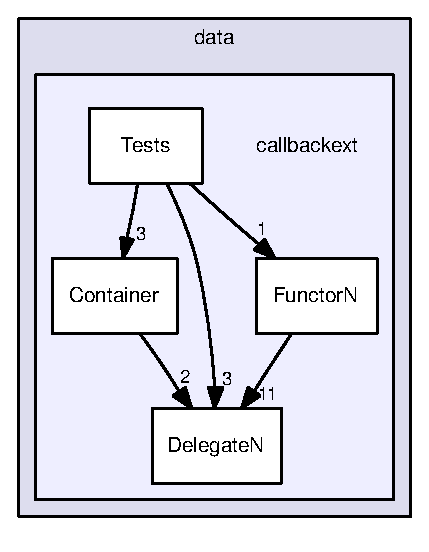
\includegraphics[width=120pt]{dir_000001_dep}
\end{center}
\end{figure}
\subsection*{Directories}
\begin{CompactItemize}
\item 
directory \hyperlink{dir_000002}{Container}
\item 
directory \hyperlink{dir_000003}{Delegate\-N}
\item 
directory \hyperlink{dir_000004}{Functor\-N}
\item 
directory \hyperlink{dir_000005}{Tests}
\end{CompactItemize}

\hypertarget{dir_000002}{
\section{/data/callbackext/Container/ Directory Reference}
\label{dir_000002}\index{/data/callbackext/Container/ Directory Reference@{/data/callbackext/Container/ Directory Reference}}
}


\begin{figure}[H]
\begin{center}
\leavevmode
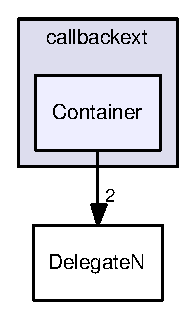
\includegraphics[width=64pt]{dir_000002_dep}
\end{center}
\end{figure}
\subsection*{Files}
\begin{CompactItemize}
\item 
file \hyperlink{AlgorithmExt_8hpp}{Algorithm\-Ext.hpp}
\item 
file \hyperlink{Associative_8hpp}{Associative.hpp}
\item 
file \hyperlink{DelegateList_8hpp}{Delegate\-List.hpp}
\end{CompactItemize}

\hypertarget{dir_000000}{
\section{/data/ Directory Reference}
\label{dir_000000}\index{/data/ Directory Reference@{/data/ Directory Reference}}
}


\begin{figure}[H]
\begin{center}
\leavevmode
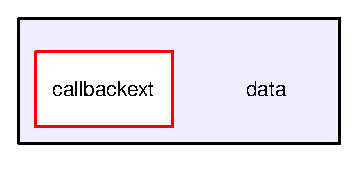
\includegraphics[width=103pt]{dir_000000_dep}
\end{center}
\end{figure}
\subsection*{Directories}
\begin{CompactItemize}
\item 
directory \hyperlink{dir_000001}{callbackext}
\end{CompactItemize}

\hypertarget{dir_000003}{
\section{/data/callbackext/Delegate\-N/ Directory Reference}
\label{dir_000003}\index{/data/callbackext/DelegateN/ Directory Reference@{/data/callbackext/DelegateN/ Directory Reference}}
}


\begin{figure}[H]
\begin{center}
\leavevmode
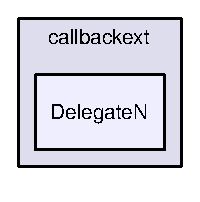
\includegraphics[width=65pt]{dir_000003_dep}
\end{center}
\end{figure}
\subsection*{Files}
\begin{CompactItemize}
\item 
file \hyperlink{Delegate0_8hpp}{Delegate0.hpp}
\item 
file \hyperlink{Delegate1_8hpp}{Delegate1.hpp}
\item 
file \hyperlink{Delegate10_8hpp}{Delegate10.hpp}
\item 
file \hyperlink{Delegate2_8hpp}{Delegate2.hpp}
\item 
file \hyperlink{Delegate3_8hpp}{Delegate3.hpp}
\item 
file \hyperlink{Delegate4_8hpp}{Delegate4.hpp}
\item 
file \hyperlink{Delegate5_8hpp}{Delegate5.hpp}
\item 
file \hyperlink{Delegate6_8hpp}{Delegate6.hpp}
\item 
file \hyperlink{Delegate7_8hpp}{Delegate7.hpp}
\item 
file \hyperlink{Delegate8_8hpp}{Delegate8.hpp}
\item 
file \hyperlink{Delegate9_8hpp}{Delegate9.hpp}
\item 
file \hyperlink{DelegateBase_8hpp}{Delegate\-Base.hpp}
\item 
file \hyperlink{DelegateN_8hpp}{Delegate\-N.hpp}
\end{CompactItemize}

\hypertarget{dir_000004}{
\section{/data/callbackext/Functor\-N/ Directory Reference}
\label{dir_000004}\index{/data/callbackext/FunctorN/ Directory Reference@{/data/callbackext/FunctorN/ Directory Reference}}
}


\begin{figure}[H]
\begin{center}
\leavevmode
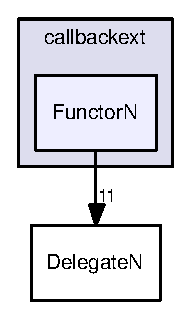
\includegraphics[width=63pt]{dir_000004_dep}
\end{center}
\end{figure}
\subsection*{Files}
\begin{CompactItemize}
\item 
file \hyperlink{Functor0_8hpp}{Functor0.hpp}
\item 
file \hyperlink{Functor1_8hpp}{Functor1.hpp}
\item 
file \hyperlink{Functor10_8hpp}{Functor10.hpp}
\item 
file \hyperlink{Functor2_8hpp}{Functor2.hpp}
\item 
file \hyperlink{Functor3_8hpp}{Functor3.hpp}
\item 
file \hyperlink{Functor4_8hpp}{Functor4.hpp}
\item 
file \hyperlink{Functor5_8hpp}{Functor5.hpp}
\item 
file \hyperlink{Functor6_8hpp}{Functor6.hpp}
\item 
file \hyperlink{Functor7_8hpp}{Functor7.hpp}
\item 
file \hyperlink{Functor8_8hpp}{Functor8.hpp}
\item 
file \hyperlink{Functor9_8hpp}{Functor9.hpp}
\item 
file \hyperlink{FunctorN_8hpp}{Functor\-N.hpp}
\end{CompactItemize}

\hypertarget{dir_000005}{
\section{/data/callbackext/Tests/ Directory Reference}
\label{dir_000005}\index{/data/callbackext/Tests/ Directory Reference@{/data/callbackext/Tests/ Directory Reference}}
}


\begin{figure}[H]
\begin{center}
\leavevmode
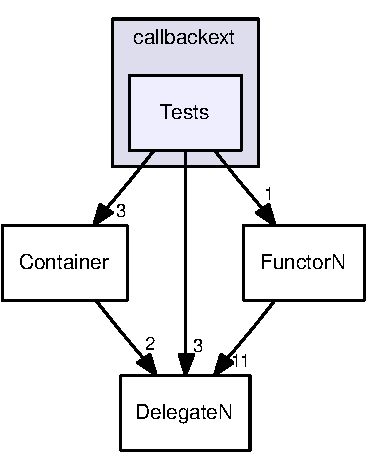
\includegraphics[width=105pt]{dir_000005_dep}
\end{center}
\end{figure}
\subsection*{Files}
\begin{CompactItemize}
\item 
file \hyperlink{DelegateTest1_8cc}{Delegate\-Test1.cc}
\item 
file \hyperlink{DelegateTest2_8cc}{Delegate\-Test2.cc}
\item 
file \hyperlink{DelegateTest3_8cc}{Delegate\-Test3.cc}
\end{CompactItemize}

\chapter{Extended C++ Callback Library Namespace Documentation}
\hypertarget{namespaceDL}{
\section{DL Namespace Reference}
\label{namespaceDL}\index{DL@{DL}}
}


\subsection*{Classes}
\begin{CompactItemize}
\item 
struct \hyperlink{structDL_1_1Deleter}{Deleter}
\item 
class \hyperlink{classDL_1_1Associative}{Associative}
\item 
class \hyperlink{classDL_1_1DelegateList}{Delegate\-List}
\item 
class \hyperlink{classDL_1_1Delegate0}{Delegate0}
\item 
class \hyperlink{classDL_1_1Delegate1}{Delegate1}
\item 
class \hyperlink{classDL_1_1Delegate10}{Delegate10}
\item 
class \hyperlink{classDL_1_1Delegate2}{Delegate2}
\item 
class \hyperlink{classDL_1_1Delegate3}{Delegate3}
\item 
class \hyperlink{classDL_1_1Delegate4}{Delegate4}
\item 
class \hyperlink{classDL_1_1Delegate5}{Delegate5}
\item 
class \hyperlink{classDL_1_1Delegate6}{Delegate6}
\item 
class \hyperlink{classDL_1_1Delegate7}{Delegate7}
\item 
class \hyperlink{classDL_1_1Delegate8}{Delegate8}
\item 
class \hyperlink{classDL_1_1Delegate9}{Delegate9}
\item 
class \hyperlink{classDL_1_1DelegateBase}{Delegate\-Base}
\item 
class \hyperlink{classDL_1_1Functor0}{Functor0}
\item 
class \hyperlink{classDL_1_1Functor1}{Functor1}
\item 
class \hyperlink{classDL_1_1Functor10}{Functor10}
\item 
class \hyperlink{classDL_1_1Functor2}{Functor2}
\item 
class \hyperlink{classDL_1_1Functor3}{Functor3}
\item 
class \hyperlink{classDL_1_1Functor4}{Functor4}
\item 
class \hyperlink{classDL_1_1Functor5}{Functor5}
\item 
class \hyperlink{classDL_1_1Functor6}{Functor6}
\item 
class \hyperlink{classDL_1_1Functor7}{Functor7}
\item 
class \hyperlink{classDL_1_1Functor8}{Functor8}
\item 
class \hyperlink{classDL_1_1Functor9}{Functor9}
\end{CompactItemize}
\subsection*{Typedefs}
\begin{CompactItemize}
\item 
typedef std::auto\_\-ptr$<$ \hyperlink{classDL_1_1DelegateBase}{Delegate\-Base} $>$ \hyperlink{namespaceDL_a0}{Delegate\-Obj}
\end{CompactItemize}
\subsection*{Functions}
\begin{CompactItemize}
\item 
template$<$class Return\-Type, class Class\-Type$>$ \hyperlink{namespaceDL_a0}{Delegate\-Obj} \hyperlink{namespaceDL_a1}{create\_\-delegate} (Class\-Type \&obj, Return\-Type(Class\-Type::$\ast$Meth)())
\item 
template$<$class Return\-Type, class Class\-Type$>$ \hyperlink{namespaceDL_a0}{Delegate\-Obj} \hyperlink{namespaceDL_a2}{create\_\-delegate} (Class\-Type $\ast$obj, Return\-Type(Class\-Type::$\ast$Meth)())
\item 
template$<$class Return\-Type, class Class\-Type, class Param1$>$ \hyperlink{namespaceDL_a0}{Delegate\-Obj} \hyperlink{namespaceDL_a3}{create\_\-delegate} (Class\-Type \&obj, Return\-Type(Class\-Type::$\ast$Meth)(Param1), Param1 \&param1)
\item 
template$<$class Return\-Type, class Class\-Type, class Param1$>$ \hyperlink{namespaceDL_a0}{Delegate\-Obj} \hyperlink{namespaceDL_a4}{create\_\-delegate} (Class\-Type $\ast$obj, Return\-Type(Class\-Type::$\ast$Meth)(Param1), Param1 \&param1)
\item 
template$<$class Return\-Type, class Class\-Type, class Param1, class Param2, class Param3, class Param4, class Param5, class Param6, class Param7, class Param8, class Param9, class Param10$>$ \hyperlink{namespaceDL_a0}{Delegate\-Obj} \hyperlink{namespaceDL_a5}{create\_\-delegate} (Class\-Type \&obj, Return\-Type(Class\-Type::$\ast$Meth)(Param1, Param2, Param3, Param4, Param5, Param6, Param7, Param8, Param9, Param10), Param1 \&param1, Param2 \&param2, Param3 \&param3, Param4 \&param4, Param5 \&param5, Param6 \&param6, Param7 \&param7, Param8 \&param8, Param9 \&param9, Param10 \&param10)
\item 
template$<$class Return\-Type, class Class\-Type, class Param1, class Param2, class Param3, class Param4, class Param5, class Param6, class Param7, class Param8, class Param9, class Param10$>$ \hyperlink{namespaceDL_a0}{Delegate\-Obj} \hyperlink{namespaceDL_a6}{create\_\-delegate} (Class\-Type $\ast$obj, Return\-Type(Class\-Type::$\ast$Meth)(Param1, Param2, Param3, Param4, Param5, Param6, Param7, Param8, Param9, Param10), Param1 \&param1, Param2 \&param2, Param3 \&param3, Param4 \&param4, Param5 \&param5, Param6 \&param6, Param7 \&param7, Param8 \&param8, Param9 \&param9, Param10 \&param10)
\item 
template$<$class Return\-Type, class Class\-Type, class Param1, class Param2$>$ \hyperlink{namespaceDL_a0}{Delegate\-Obj} \hyperlink{namespaceDL_a7}{create\_\-delegate} (Class\-Type \&obj, Return\-Type(Class\-Type::$\ast$Meth)(Param1, Param2), Param1 \&param1, Param2 \&param2)
\item 
template$<$class Return\-Type, class Class\-Type, class Param1, class Param2$>$ \hyperlink{namespaceDL_a0}{Delegate\-Obj} \hyperlink{namespaceDL_a8}{create\_\-delegate} (Class\-Type $\ast$obj, Return\-Type(Class\-Type::$\ast$Meth)(Param1, Param2), Param1 \&param1, Param2 \&param2)
\item 
template$<$class Return\-Type, class Class\-Type, class Param1, class Param2, class Param3$>$ \hyperlink{namespaceDL_a0}{Delegate\-Obj} \hyperlink{namespaceDL_a9}{create\_\-delegate} (Class\-Type \&obj, Return\-Type(Class\-Type::$\ast$Meth)(Param1, Param2, Param3), Param1 \&param1, Param2 \&param2, Param3 \&param3)
\item 
template$<$class Return\-Type, class Class\-Type, class Param1, class Param2, class Param3$>$ \hyperlink{namespaceDL_a0}{Delegate\-Obj} \hyperlink{namespaceDL_a10}{create\_\-delegate} (Class\-Type $\ast$obj, Return\-Type(Class\-Type::$\ast$Meth)(Param1, Param2, Param3), Param1 \&param1, Param2 \&param2, Param3 \&param3)
\item 
template$<$class Return\-Type, class Class\-Type, class Param1, class Param2, class Param3, class Param4$>$ \hyperlink{namespaceDL_a0}{Delegate\-Obj} \hyperlink{namespaceDL_a11}{create\_\-delegate} (Class\-Type \&obj, Return\-Type(Class\-Type::$\ast$Meth)(Param1, Param2, Param3, Param4), Param1 \&param1, Param2 \&param2, Param3 \&param3, Param4 \&param4)
\item 
template$<$class Return\-Type, class Class\-Type, class Param1, class Param2, class Param3, class Param4$>$ \hyperlink{namespaceDL_a0}{Delegate\-Obj} \hyperlink{namespaceDL_a12}{create\_\-delegate} (Class\-Type $\ast$obj, Return\-Type(Class\-Type::$\ast$Meth)(Param1, Param2, Param3, Param4), Param1 \&param1, Param2 \&param2, Param3 \&param3, Param4 \&param4)
\item 
template$<$class Return\-Type, class Class\-Type, class Param1, class Param2, class Param3, class Param4, class Param5$>$ \hyperlink{namespaceDL_a0}{Delegate\-Obj} \hyperlink{namespaceDL_a13}{create\_\-delegate} (Class\-Type \&obj, Return\-Type(Class\-Type::$\ast$Meth)(Param1, Param2, Param3, Param4, Param5), Param1 \&param1, Param2 \&param2, Param3 \&param3, Param4 \&param4, Param5 \&param5)
\item 
template$<$class Return\-Type, class Class\-Type, class Param1, class Param2, class Param3, class Param4, class Param5$>$ \hyperlink{namespaceDL_a0}{Delegate\-Obj} \hyperlink{namespaceDL_a14}{create\_\-delegate} (Class\-Type $\ast$obj, Return\-Type(Class\-Type::$\ast$Meth)(Param1, Param2, Param3, Param4, Param5), Param1 \&param1, Param2 \&param2, Param3 \&param3, Param4 \&param4, Param5 \&param5)
\item 
template$<$class Return\-Type, class Class\-Type, class Param1, class Param2, class Param3, class Param4, class Param5, class Param6$>$ \hyperlink{namespaceDL_a0}{Delegate\-Obj} \hyperlink{namespaceDL_a15}{create\_\-delegate} (Class\-Type \&obj, Return\-Type(Class\-Type::$\ast$Meth)(Param1, Param2, Param3, Param4, Param5, Param6), Param1 \&param1, Param2 \&param2, Param3 \&param3, Param4 \&param4, Param5 \&param5, Param6 \&param6)
\item 
template$<$class Return\-Type, class Class\-Type, class Param1, class Param2, class Param3, class Param4, class Param5, class Param6$>$ \hyperlink{namespaceDL_a0}{Delegate\-Obj} \hyperlink{namespaceDL_a16}{create\_\-delegate} (Class\-Type $\ast$obj, Return\-Type(Class\-Type::$\ast$Meth)(Param1, Param2, Param3, Param4, Param5, Param6), Param1 \&param1, Param2 \&param2, Param3 \&param3, Param4 \&param4, Param5 \&param5, Param6 \&param6)
\item 
template$<$class Return\-Type, class Class\-Type, class Param1, class Param2, class Param3, class Param4, class Param5, class Param6, class Param7$>$ \hyperlink{namespaceDL_a0}{Delegate\-Obj} \hyperlink{namespaceDL_a17}{create\_\-delegate} (Class\-Type \&obj, Return\-Type(Class\-Type::$\ast$Meth)(Param1, Param2, Param3, Param4, Param5, Param6, Param7), Param1 \&param1, Param2 \&param2, Param3 \&param3, Param4 \&param4, Param5 \&param5, Param6 \&param6, Param7 \&param7)
\item 
template$<$class Return\-Type, class Class\-Type, class Param1, class Param2, class Param3, class Param4, class Param5, class Param6, class Param7$>$ \hyperlink{namespaceDL_a0}{Delegate\-Obj} \hyperlink{namespaceDL_a18}{create\_\-delegate} (Class\-Type $\ast$obj, Return\-Type(Class\-Type::$\ast$Meth)(Param1, Param2, Param3, Param4, Param5, Param6, Param7), Param1 \&param1, Param2 \&param2, Param3 \&param3, Param4 \&param4, Param5 \&param5, Param6 \&param6, Param7 \&param7)
\item 
template$<$class Return\-Type, class Class\-Type, class Param1, class Param2, class Param3, class Param4, class Param5, class Param6, class Param7, class Param8$>$ \hyperlink{namespaceDL_a0}{Delegate\-Obj} \hyperlink{namespaceDL_a19}{create\_\-delegate} (Class\-Type \&obj, Return\-Type(Class\-Type::$\ast$Meth)(Param1, Param2, Param3, Param4, Param5, Param6, Param7, Param8), Param1 \&param1, Param2 \&param2, Param3 \&param3, Param4 \&param4, Param5 \&param5, Param6 \&param6, Param7 \&param7, Param8 \&param8)
\item 
template$<$class Return\-Type, class Class\-Type, class Param1, class Param2, class Param3, class Param4, class Param5, class Param6, class Param7, class Param8$>$ \hyperlink{namespaceDL_a0}{Delegate\-Obj} \hyperlink{namespaceDL_a20}{create\_\-delegate} (Class\-Type $\ast$obj, Return\-Type(Class\-Type::$\ast$Meth)(Param1, Param2, Param3, Param4, Param5, Param6, Param7, Param8), Param1 \&param1, Param2 \&param2, Param3 \&param3, Param4 \&param4, Param5 \&param5, Param6 \&param6, Param7 \&param7, Param8 \&param8)
\item 
template$<$class Return\-Type, class Class\-Type, class Param1, class Param2, class Param3, class Param4, class Param5, class Param6, class Param7, class Param8, class Param9$>$ \hyperlink{namespaceDL_a0}{Delegate\-Obj} \hyperlink{namespaceDL_a21}{create\_\-delegate} (Class\-Type \&obj, Return\-Type(Class\-Type::$\ast$Meth)(Param1, Param2, Param3, Param4, Param5, Param6, Param7, Param8, Param9), Param1 \&param1, Param2 \&param2, Param3 \&param3, Param4 \&param4, Param5 \&param5, Param6 \&param6, Param7 \&param7, Param8 \&param8, Param9 \&param9)
\item 
template$<$class Return\-Type, class Class\-Type, class Param1, class Param2, class Param3, class Param4, class Param5, class Param6, class Param7, class Param8, class Param9$>$ \hyperlink{namespaceDL_a0}{Delegate\-Obj} \hyperlink{namespaceDL_a22}{create\_\-delegate} (Class\-Type $\ast$obj, Return\-Type(Class\-Type::$\ast$Meth)(Param1, Param2, Param3, Param4, Param5, Param6, Param7, Param8, Param9), Param1 \&param1, Param2 \&param2, Param3 \&param3, Param4 \&param4, Param5 \&param5, Param6 \&param6, Param7 \&param7, Param8 \&param8, Param9 \&param9)
\item 
\hyperlink{namespaceDL_a0}{Delegate\-Obj} \hyperlink{namespaceDL_a23}{create\_\-delegate} (void($\ast$Meth)(void))
\item 
template$<$class Return\-Type, class Param1$>$ \hyperlink{namespaceDL_a0}{Delegate\-Obj} \hyperlink{namespaceDL_a24}{create\_\-delegate} (Return\-Type($\ast$Meth)(Param1), Param1 \&param1)
\item 
template$<$class Return\-Type, class Param1, class Param2, class Param3, class Param4, class Param5, class Param6, class Param7, class Param8, class Param9, class Param10$>$ \hyperlink{namespaceDL_a0}{Delegate\-Obj} \hyperlink{namespaceDL_a25}{create\_\-delegate} (Return\-Type($\ast$Meth)(Param1, Param2, Param3, Param4, Param5, Param6, Param7, Param8, Param9, Param10), Param1 \&param1, Param2 \&param2, Param3 \&param3, Param4 \&param4, Param5 \&param5, Param6 \&param6, Param7 \&param7, Param8 \&param8, Param9 \&param9, Param10 \&param10)
\item 
template$<$class Return\-Type, class Param1, class Param2$>$ \hyperlink{namespaceDL_a0}{Delegate\-Obj} \hyperlink{namespaceDL_a26}{create\_\-delegate} (Return\-Type($\ast$Meth)(Param1, Param2), Param1 \&param1, Param2 \&param2)
\item 
template$<$class Return\-Type, class Param1, class Param2, class Param3$>$ \hyperlink{namespaceDL_a0}{Delegate\-Obj} \hyperlink{namespaceDL_a27}{create\_\-delegate} (Return\-Type($\ast$Meth)(Param1, Param2, Param3), Param1 \&param1, Param2 \&param2, Param3 \&param3)
\item 
template$<$class Return\-Type, class Param1, class Param2, class Param3, class Param4$>$ \hyperlink{namespaceDL_a0}{Delegate\-Obj} \hyperlink{namespaceDL_a28}{create\_\-delegate} (Return\-Type($\ast$Meth)(Param1, Param2, Param3, Param4), Param1 \&param1, Param2 \&param2, Param3 \&param3, Param4 \&param4)
\item 
template$<$class Return\-Type, class Param1, class Param2, class Param3, class Param4, class Param5$>$ \hyperlink{namespaceDL_a0}{Delegate\-Obj} \hyperlink{namespaceDL_a29}{create\_\-delegate} (Return\-Type($\ast$Meth)(Param1, Param2, Param3, Param4, Param5), Param1 \&param1, Param2 \&param2, Param3 \&param3, Param4 \&param4, Param5 \&param5)
\item 
template$<$class Return\-Type, class Param1, class Param2, class Param3, class Param4, class Param5, class Param6$>$ \hyperlink{namespaceDL_a0}{Delegate\-Obj} \hyperlink{namespaceDL_a30}{create\_\-delegate} (Return\-Type($\ast$Meth)(Param1, Param2, Param3, Param4, Param5, Param6), Param1 \&param1, Param2 \&param2, Param3 \&param3, Param4 \&param4, Param5 \&param5, Param6 \&param6)
\item 
template$<$class Return\-Type, class Param1, class Param2, class Param3, class Param4, class Param5, class Param6, class Param7$>$ \hyperlink{namespaceDL_a0}{Delegate\-Obj} \hyperlink{namespaceDL_a31}{create\_\-delegate} (Return\-Type($\ast$Meth)(Param1, Param2, Param3, Param4, Param5, Param6, Param7), Param1 \&param1, Param2 \&param2, Param3 \&param3, Param4 \&param4, Param5 \&param5, Param6 \&param6, Param7 \&param7)
\item 
template$<$class Return\-Type, class Param1, class Param2, class Param3, class Param4, class Param5, class Param6, class Param7, class Param8$>$ \hyperlink{namespaceDL_a0}{Delegate\-Obj} \hyperlink{namespaceDL_a32}{create\_\-delegate} (Return\-Type($\ast$Meth)(Param1, Param2, Param3, Param4, Param5, Param6, Param7, Param8), Param1 \&param1, Param2 \&param2, Param3 \&param3, Param4 \&param4, Param5 \&param5, Param6 \&param6, Param7 \&param7, Param8 \&param8)
\item 
template$<$class Return\-Type, class Param1, class Param2, class Param3, class Param4, class Param5, class Param6, class Param7, class Param8, class Param9$>$ \hyperlink{namespaceDL_a0}{Delegate\-Obj} \hyperlink{namespaceDL_a33}{create\_\-delegate} (Return\-Type($\ast$Meth)(Param1, Param2, Param3, Param4, Param5, Param6, Param7, Param8, Param9), Param1 \&param1, Param2 \&param2, Param3 \&param3, Param4 \&param4, Param5 \&param5, Param6 \&param6, Param7 \&param7, Param8 \&param8, Param9 \&param9)
\end{CompactItemize}


\subsection{Detailed Description}
\hyperlink{classDL_1_1DelegateList}{Delegate\-List} is a Method Pointer Container 



\subsection{Typedef Documentation}
\hypertarget{namespaceDL_a0}{
\index{DL@{DL}!DelegateObj@{DelegateObj}}
\index{DelegateObj@{DelegateObj}!DL@{DL}}
\subsubsection[DelegateObj]{\setlength{\rightskip}{0pt plus 5cm}typedef std::auto\_\-ptr$<$\hyperlink{classDL_1_1DelegateBase}{Delegate\-Base}$>$ \hyperlink{namespaceDL_a0}{DL::Delegate\-Obj}}}
\label{namespaceDL_a0}




Definition at line 33 of file Delegate\-Base.hpp.

\subsection{Function Documentation}
\hypertarget{namespaceDL_a33}{
\index{DL@{DL}!create_delegate@{create\_\-delegate}}
\index{create_delegate@{create\_\-delegate}!DL@{DL}}
\subsubsection[create\_\-delegate]{\setlength{\rightskip}{0pt plus 5cm}template$<$class Return\-Type, class Param1, class Param2, class Param3, class Param4, class Param5, class Param6, class Param7, class Param8, class Param9$>$ \hyperlink{namespaceDL_a0}{Delegate\-Obj} create\_\-delegate (Return\-Type($\ast$)(Param1, Param2, Param3, Param4, Param5, Param6, Param7, Param8, Param9) {\em Meth}, Param1 \& {\em param1}, Param2 \& {\em param2}, Param3 \& {\em param3}, Param4 \& {\em param4}, Param5 \& {\em param5}, Param6 \& {\em param6}, Param7 \& {\em param7}, Param8 \& {\em param8}, Param9 \& {\em param9})}}
\label{namespaceDL_a33}




Definition at line 85 of file Functor9.hpp.\hypertarget{namespaceDL_a32}{
\index{DL@{DL}!create_delegate@{create\_\-delegate}}
\index{create_delegate@{create\_\-delegate}!DL@{DL}}
\subsubsection[create\_\-delegate]{\setlength{\rightskip}{0pt plus 5cm}template$<$class Return\-Type, class Param1, class Param2, class Param3, class Param4, class Param5, class Param6, class Param7, class Param8$>$ \hyperlink{namespaceDL_a0}{Delegate\-Obj} create\_\-delegate (Return\-Type($\ast$)(Param1, Param2, Param3, Param4, Param5, Param6, Param7, Param8) {\em Meth}, Param1 \& {\em param1}, Param2 \& {\em param2}, Param3 \& {\em param3}, Param4 \& {\em param4}, Param5 \& {\em param5}, Param6 \& {\em param6}, Param7 \& {\em param7}, Param8 \& {\em param8})}}
\label{namespaceDL_a32}




Definition at line 82 of file Functor8.hpp.\hypertarget{namespaceDL_a31}{
\index{DL@{DL}!create_delegate@{create\_\-delegate}}
\index{create_delegate@{create\_\-delegate}!DL@{DL}}
\subsubsection[create\_\-delegate]{\setlength{\rightskip}{0pt plus 5cm}template$<$class Return\-Type, class Param1, class Param2, class Param3, class Param4, class Param5, class Param6, class Param7$>$ \hyperlink{namespaceDL_a0}{Delegate\-Obj} create\_\-delegate (Return\-Type($\ast$)(Param1, Param2, Param3, Param4, Param5, Param6, Param7) {\em Meth}, Param1 \& {\em param1}, Param2 \& {\em param2}, Param3 \& {\em param3}, Param4 \& {\em param4}, Param5 \& {\em param5}, Param6 \& {\em param6}, Param7 \& {\em param7})}}
\label{namespaceDL_a31}




Definition at line 78 of file Functor7.hpp.\hypertarget{namespaceDL_a30}{
\index{DL@{DL}!create_delegate@{create\_\-delegate}}
\index{create_delegate@{create\_\-delegate}!DL@{DL}}
\subsubsection[create\_\-delegate]{\setlength{\rightskip}{0pt plus 5cm}template$<$class Return\-Type, class Param1, class Param2, class Param3, class Param4, class Param5, class Param6$>$ \hyperlink{namespaceDL_a0}{Delegate\-Obj} create\_\-delegate (Return\-Type($\ast$)(Param1, Param2, Param3, Param4, Param5, Param6) {\em Meth}, Param1 \& {\em param1}, Param2 \& {\em param2}, Param3 \& {\em param3}, Param4 \& {\em param4}, Param5 \& {\em param5}, Param6 \& {\em param6})}}
\label{namespaceDL_a30}




Definition at line 74 of file Functor6.hpp.\hypertarget{namespaceDL_a29}{
\index{DL@{DL}!create_delegate@{create\_\-delegate}}
\index{create_delegate@{create\_\-delegate}!DL@{DL}}
\subsubsection[create\_\-delegate]{\setlength{\rightskip}{0pt plus 5cm}template$<$class Return\-Type, class Param1, class Param2, class Param3, class Param4, class Param5$>$ \hyperlink{namespaceDL_a0}{Delegate\-Obj} create\_\-delegate (Return\-Type($\ast$)(Param1, Param2, Param3, Param4, Param5) {\em Meth}, Param1 \& {\em param1}, Param2 \& {\em param2}, Param3 \& {\em param3}, Param4 \& {\em param4}, Param5 \& {\em param5})}}
\label{namespaceDL_a29}




Definition at line 71 of file Functor5.hpp.\hypertarget{namespaceDL_a28}{
\index{DL@{DL}!create_delegate@{create\_\-delegate}}
\index{create_delegate@{create\_\-delegate}!DL@{DL}}
\subsubsection[create\_\-delegate]{\setlength{\rightskip}{0pt plus 5cm}template$<$class Return\-Type, class Param1, class Param2, class Param3, class Param4$>$ \hyperlink{namespaceDL_a0}{Delegate\-Obj} create\_\-delegate (Return\-Type($\ast$)(Param1, Param2, Param3, Param4) {\em Meth}, Param1 \& {\em param1}, Param2 \& {\em param2}, Param3 \& {\em param3}, Param4 \& {\em param4})}}
\label{namespaceDL_a28}




Definition at line 66 of file Functor4.hpp.\hypertarget{namespaceDL_a27}{
\index{DL@{DL}!create_delegate@{create\_\-delegate}}
\index{create_delegate@{create\_\-delegate}!DL@{DL}}
\subsubsection[create\_\-delegate]{\setlength{\rightskip}{0pt plus 5cm}template$<$class Return\-Type, class Param1, class Param2, class Param3$>$ \hyperlink{namespaceDL_a0}{Delegate\-Obj} create\_\-delegate (Return\-Type($\ast$)(Param1, Param2, Param3) {\em Meth}, Param1 \& {\em param1}, Param2 \& {\em param2}, Param3 \& {\em param3})}}
\label{namespaceDL_a27}




Definition at line 63 of file Functor3.hpp.\hypertarget{namespaceDL_a26}{
\index{DL@{DL}!create_delegate@{create\_\-delegate}}
\index{create_delegate@{create\_\-delegate}!DL@{DL}}
\subsubsection[create\_\-delegate]{\setlength{\rightskip}{0pt plus 5cm}template$<$class Return\-Type, class Param1, class Param2$>$ \hyperlink{namespaceDL_a0}{Delegate\-Obj} create\_\-delegate (Return\-Type($\ast$)(Param1, Param2) {\em Meth}, Param1 \& {\em param1}, Param2 \& {\em param2})}}
\label{namespaceDL_a26}




Definition at line 60 of file Functor2.hpp.\hypertarget{namespaceDL_a25}{
\index{DL@{DL}!create_delegate@{create\_\-delegate}}
\index{create_delegate@{create\_\-delegate}!DL@{DL}}
\subsubsection[create\_\-delegate]{\setlength{\rightskip}{0pt plus 5cm}template$<$class Return\-Type, class Param1, class Param2, class Param3, class Param4, class Param5, class Param6, class Param7, class Param8, class Param9, class Param10$>$ \hyperlink{namespaceDL_a0}{Delegate\-Obj} create\_\-delegate (Return\-Type($\ast$)(Param1, Param2, Param3, Param4, Param5, Param6, Param7, Param8, Param9, Param10) {\em Meth}, Param1 \& {\em param1}, Param2 \& {\em param2}, Param3 \& {\em param3}, Param4 \& {\em param4}, Param5 \& {\em param5}, Param6 \& {\em param6}, Param7 \& {\em param7}, Param8 \& {\em param8}, Param9 \& {\em param9}, Param10 \& {\em param10})}}
\label{namespaceDL_a25}




Definition at line 89 of file Functor10.hpp.\hypertarget{namespaceDL_a24}{
\index{DL@{DL}!create_delegate@{create\_\-delegate}}
\index{create_delegate@{create\_\-delegate}!DL@{DL}}
\subsubsection[create\_\-delegate]{\setlength{\rightskip}{0pt plus 5cm}template$<$class Return\-Type, class Param1$>$ \hyperlink{namespaceDL_a0}{Delegate\-Obj} create\_\-delegate (Return\-Type($\ast$)(Param1) {\em Meth}, Param1 \& {\em param1})}}
\label{namespaceDL_a24}




Definition at line 54 of file Functor1.hpp.\hypertarget{namespaceDL_a23}{
\index{DL@{DL}!create_delegate@{create\_\-delegate}}
\index{create_delegate@{create\_\-delegate}!DL@{DL}}
\subsubsection[create\_\-delegate]{\setlength{\rightskip}{0pt plus 5cm}\hyperlink{namespaceDL_a0}{Delegate\-Obj} create\_\-delegate (void($\ast$)(void) {\em Meth})}}
\label{namespaceDL_a23}




Definition at line 46 of file Functor0.hpp.\hypertarget{namespaceDL_a22}{
\index{DL@{DL}!create_delegate@{create\_\-delegate}}
\index{create_delegate@{create\_\-delegate}!DL@{DL}}
\subsubsection[create\_\-delegate]{\setlength{\rightskip}{0pt plus 5cm}template$<$class Return\-Type, class Class\-Type, class Param1, class Param2, class Param3, class Param4, class Param5, class Param6, class Param7, class Param8, class Param9$>$ \hyperlink{namespaceDL_a0}{Delegate\-Obj} create\_\-delegate (Class\-Type $\ast$ {\em obj}, Return\-Type(Class\-Type::$\ast$)(Param1, Param2, Param3, Param4, Param5, Param6, Param7, Param8, Param9) {\em Meth}, Param1 \& {\em param1}, Param2 \& {\em param2}, Param3 \& {\em param3}, Param4 \& {\em param4}, Param5 \& {\em param5}, Param6 \& {\em param6}, Param7 \& {\em param7}, Param8 \& {\em param8}, Param9 \& {\em param9})}}
\label{namespaceDL_a22}




Definition at line 102 of file Delegate9.hpp.\hypertarget{namespaceDL_a21}{
\index{DL@{DL}!create_delegate@{create\_\-delegate}}
\index{create_delegate@{create\_\-delegate}!DL@{DL}}
\subsubsection[create\_\-delegate]{\setlength{\rightskip}{0pt plus 5cm}template$<$class Return\-Type, class Class\-Type, class Param1, class Param2, class Param3, class Param4, class Param5, class Param6, class Param7, class Param8, class Param9$>$ \hyperlink{namespaceDL_a0}{Delegate\-Obj} create\_\-delegate (Class\-Type \& {\em obj}, Return\-Type(Class\-Type::$\ast$)(Param1, Param2, Param3, Param4, Param5, Param6, Param7, Param8, Param9) {\em Meth}, Param1 \& {\em param1}, Param2 \& {\em param2}, Param3 \& {\em param3}, Param4 \& {\em param4}, Param5 \& {\em param5}, Param6 \& {\em param6}, Param7 \& {\em param7}, Param8 \& {\em param8}, Param9 \& {\em param9})}}
\label{namespaceDL_a21}




Definition at line 88 of file Delegate9.hpp.\hypertarget{namespaceDL_a20}{
\index{DL@{DL}!create_delegate@{create\_\-delegate}}
\index{create_delegate@{create\_\-delegate}!DL@{DL}}
\subsubsection[create\_\-delegate]{\setlength{\rightskip}{0pt plus 5cm}template$<$class Return\-Type, class Class\-Type, class Param1, class Param2, class Param3, class Param4, class Param5, class Param6, class Param7, class Param8$>$ \hyperlink{namespaceDL_a0}{Delegate\-Obj} create\_\-delegate (Class\-Type $\ast$ {\em obj}, Return\-Type(Class\-Type::$\ast$)(Param1, Param2, Param3, Param4, Param5, Param6, Param7, Param8) {\em Meth}, Param1 \& {\em param1}, Param2 \& {\em param2}, Param3 \& {\em param3}, Param4 \& {\em param4}, Param5 \& {\em param5}, Param6 \& {\em param6}, Param7 \& {\em param7}, Param8 \& {\em param8})}}
\label{namespaceDL_a20}




Definition at line 98 of file Delegate8.hpp.\hypertarget{namespaceDL_a19}{
\index{DL@{DL}!create_delegate@{create\_\-delegate}}
\index{create_delegate@{create\_\-delegate}!DL@{DL}}
\subsubsection[create\_\-delegate]{\setlength{\rightskip}{0pt plus 5cm}template$<$class Return\-Type, class Class\-Type, class Param1, class Param2, class Param3, class Param4, class Param5, class Param6, class Param7, class Param8$>$ \hyperlink{namespaceDL_a0}{Delegate\-Obj} create\_\-delegate (Class\-Type \& {\em obj}, Return\-Type(Class\-Type::$\ast$)(Param1, Param2, Param3, Param4, Param5, Param6, Param7, Param8) {\em Meth}, Param1 \& {\em param1}, Param2 \& {\em param2}, Param3 \& {\em param3}, Param4 \& {\em param4}, Param5 \& {\em param5}, Param6 \& {\em param6}, Param7 \& {\em param7}, Param8 \& {\em param8})}}
\label{namespaceDL_a19}




Definition at line 84 of file Delegate8.hpp.\hypertarget{namespaceDL_a18}{
\index{DL@{DL}!create_delegate@{create\_\-delegate}}
\index{create_delegate@{create\_\-delegate}!DL@{DL}}
\subsubsection[create\_\-delegate]{\setlength{\rightskip}{0pt plus 5cm}template$<$class Return\-Type, class Class\-Type, class Param1, class Param2, class Param3, class Param4, class Param5, class Param6, class Param7$>$ \hyperlink{namespaceDL_a0}{Delegate\-Obj} create\_\-delegate (Class\-Type $\ast$ {\em obj}, Return\-Type(Class\-Type::$\ast$)(Param1, Param2, Param3, Param4, Param5, Param6, Param7) {\em Meth}, Param1 \& {\em param1}, Param2 \& {\em param2}, Param3 \& {\em param3}, Param4 \& {\em param4}, Param5 \& {\em param5}, Param6 \& {\em param6}, Param7 \& {\em param7})}}
\label{namespaceDL_a18}




Definition at line 94 of file Delegate7.hpp.\hypertarget{namespaceDL_a17}{
\index{DL@{DL}!create_delegate@{create\_\-delegate}}
\index{create_delegate@{create\_\-delegate}!DL@{DL}}
\subsubsection[create\_\-delegate]{\setlength{\rightskip}{0pt plus 5cm}template$<$class Return\-Type, class Class\-Type, class Param1, class Param2, class Param3, class Param4, class Param5, class Param6, class Param7$>$ \hyperlink{namespaceDL_a0}{Delegate\-Obj} create\_\-delegate (Class\-Type \& {\em obj}, Return\-Type(Class\-Type::$\ast$)(Param1, Param2, Param3, Param4, Param5, Param6, Param7) {\em Meth}, Param1 \& {\em param1}, Param2 \& {\em param2}, Param3 \& {\em param3}, Param4 \& {\em param4}, Param5 \& {\em param5}, Param6 \& {\em param6}, Param7 \& {\em param7})}}
\label{namespaceDL_a17}




Definition at line 81 of file Delegate7.hpp.\hypertarget{namespaceDL_a16}{
\index{DL@{DL}!create_delegate@{create\_\-delegate}}
\index{create_delegate@{create\_\-delegate}!DL@{DL}}
\subsubsection[create\_\-delegate]{\setlength{\rightskip}{0pt plus 5cm}template$<$class Return\-Type, class Class\-Type, class Param1, class Param2, class Param3, class Param4, class Param5, class Param6$>$ \hyperlink{namespaceDL_a0}{Delegate\-Obj} create\_\-delegate (Class\-Type $\ast$ {\em obj}, Return\-Type(Class\-Type::$\ast$)(Param1, Param2, Param3, Param4, Param5, Param6) {\em Meth}, Param1 \& {\em param1}, Param2 \& {\em param2}, Param3 \& {\em param3}, Param4 \& {\em param4}, Param5 \& {\em param5}, Param6 \& {\em param6})}}
\label{namespaceDL_a16}




Definition at line 89 of file Delegate6.hpp.\hypertarget{namespaceDL_a15}{
\index{DL@{DL}!create_delegate@{create\_\-delegate}}
\index{create_delegate@{create\_\-delegate}!DL@{DL}}
\subsubsection[create\_\-delegate]{\setlength{\rightskip}{0pt plus 5cm}template$<$class Return\-Type, class Class\-Type, class Param1, class Param2, class Param3, class Param4, class Param5, class Param6$>$ \hyperlink{namespaceDL_a0}{Delegate\-Obj} create\_\-delegate (Class\-Type \& {\em obj}, Return\-Type(Class\-Type::$\ast$)(Param1, Param2, Param3, Param4, Param5, Param6) {\em Meth}, Param1 \& {\em param1}, Param2 \& {\em param2}, Param3 \& {\em param3}, Param4 \& {\em param4}, Param5 \& {\em param5}, Param6 \& {\em param6})}}
\label{namespaceDL_a15}




Definition at line 77 of file Delegate6.hpp.\hypertarget{namespaceDL_a14}{
\index{DL@{DL}!create_delegate@{create\_\-delegate}}
\index{create_delegate@{create\_\-delegate}!DL@{DL}}
\subsubsection[create\_\-delegate]{\setlength{\rightskip}{0pt plus 5cm}template$<$class Return\-Type, class Class\-Type, class Param1, class Param2, class Param3, class Param4, class Param5$>$ \hyperlink{namespaceDL_a0}{Delegate\-Obj} create\_\-delegate (Class\-Type $\ast$ {\em obj}, Return\-Type(Class\-Type::$\ast$)(Param1, Param2, Param3, Param4, Param5) {\em Meth}, Param1 \& {\em param1}, Param2 \& {\em param2}, Param3 \& {\em param3}, Param4 \& {\em param4}, Param5 \& {\em param5})}}
\label{namespaceDL_a14}




Definition at line 86 of file Delegate5.hpp.\hypertarget{namespaceDL_a13}{
\index{DL@{DL}!create_delegate@{create\_\-delegate}}
\index{create_delegate@{create\_\-delegate}!DL@{DL}}
\subsubsection[create\_\-delegate]{\setlength{\rightskip}{0pt plus 5cm}template$<$class Return\-Type, class Class\-Type, class Param1, class Param2, class Param3, class Param4, class Param5$>$ \hyperlink{namespaceDL_a0}{Delegate\-Obj} create\_\-delegate (Class\-Type \& {\em obj}, Return\-Type(Class\-Type::$\ast$)(Param1, Param2, Param3, Param4, Param5) {\em Meth}, Param1 \& {\em param1}, Param2 \& {\em param2}, Param3 \& {\em param3}, Param4 \& {\em param4}, Param5 \& {\em param5})}}
\label{namespaceDL_a13}




Definition at line 74 of file Delegate5.hpp.\hypertarget{namespaceDL_a12}{
\index{DL@{DL}!create_delegate@{create\_\-delegate}}
\index{create_delegate@{create\_\-delegate}!DL@{DL}}
\subsubsection[create\_\-delegate]{\setlength{\rightskip}{0pt plus 5cm}template$<$class Return\-Type, class Class\-Type, class Param1, class Param2, class Param3, class Param4$>$ \hyperlink{namespaceDL_a0}{Delegate\-Obj} create\_\-delegate (Class\-Type $\ast$ {\em obj}, Return\-Type(Class\-Type::$\ast$)(Param1, Param2, Param3, Param4) {\em Meth}, Param1 \& {\em param1}, Param2 \& {\em param2}, Param3 \& {\em param3}, Param4 \& {\em param4})}}
\label{namespaceDL_a12}




Definition at line 78 of file Delegate4.hpp.\hypertarget{namespaceDL_a11}{
\index{DL@{DL}!create_delegate@{create\_\-delegate}}
\index{create_delegate@{create\_\-delegate}!DL@{DL}}
\subsubsection[create\_\-delegate]{\setlength{\rightskip}{0pt plus 5cm}template$<$class Return\-Type, class Class\-Type, class Param1, class Param2, class Param3, class Param4$>$ \hyperlink{namespaceDL_a0}{Delegate\-Obj} create\_\-delegate (Class\-Type \& {\em obj}, Return\-Type(Class\-Type::$\ast$)(Param1, Param2, Param3, Param4) {\em Meth}, Param1 \& {\em param1}, Param2 \& {\em param2}, Param3 \& {\em param3}, Param4 \& {\em param4})}}
\label{namespaceDL_a11}




Definition at line 70 of file Delegate4.hpp.\hypertarget{namespaceDL_a10}{
\index{DL@{DL}!create_delegate@{create\_\-delegate}}
\index{create_delegate@{create\_\-delegate}!DL@{DL}}
\subsubsection[create\_\-delegate]{\setlength{\rightskip}{0pt plus 5cm}template$<$class Return\-Type, class Class\-Type, class Param1, class Param2, class Param3$>$ \hyperlink{namespaceDL_a0}{Delegate\-Obj} create\_\-delegate (Class\-Type $\ast$ {\em obj}, Return\-Type(Class\-Type::$\ast$)(Param1, Param2, Param3) {\em Meth}, Param1 \& {\em param1}, Param2 \& {\em param2}, Param3 \& {\em param3})}}
\label{namespaceDL_a10}




Definition at line 76 of file Delegate3.hpp.\hypertarget{namespaceDL_a9}{
\index{DL@{DL}!create_delegate@{create\_\-delegate}}
\index{create_delegate@{create\_\-delegate}!DL@{DL}}
\subsubsection[create\_\-delegate]{\setlength{\rightskip}{0pt plus 5cm}template$<$class Return\-Type, class Class\-Type, class Param1, class Param2, class Param3$>$ \hyperlink{namespaceDL_a0}{Delegate\-Obj} create\_\-delegate (Class\-Type \& {\em obj}, Return\-Type(Class\-Type::$\ast$)(Param1, Param2, Param3) {\em Meth}, Param1 \& {\em param1}, Param2 \& {\em param2}, Param3 \& {\em param3})}}
\label{namespaceDL_a9}




Definition at line 68 of file Delegate3.hpp.\hypertarget{namespaceDL_a8}{
\index{DL@{DL}!create_delegate@{create\_\-delegate}}
\index{create_delegate@{create\_\-delegate}!DL@{DL}}
\subsubsection[create\_\-delegate]{\setlength{\rightskip}{0pt plus 5cm}template$<$class Return\-Type, class Class\-Type, class Param1, class Param2$>$ \hyperlink{namespaceDL_a0}{Delegate\-Obj} create\_\-delegate (Class\-Type $\ast$ {\em obj}, Return\-Type(Class\-Type::$\ast$)(Param1, Param2) {\em Meth}, Param1 \& {\em param1}, Param2 \& {\em param2})}}
\label{namespaceDL_a8}




Definition at line 68 of file Delegate2.hpp.\hypertarget{namespaceDL_a7}{
\index{DL@{DL}!create_delegate@{create\_\-delegate}}
\index{create_delegate@{create\_\-delegate}!DL@{DL}}
\subsubsection[create\_\-delegate]{\setlength{\rightskip}{0pt plus 5cm}template$<$class Return\-Type, class Class\-Type, class Param1, class Param2$>$ \hyperlink{namespaceDL_a0}{Delegate\-Obj} create\_\-delegate (Class\-Type \& {\em obj}, Return\-Type(Class\-Type::$\ast$)(Param1, Param2) {\em Meth}, Param1 \& {\em param1}, Param2 \& {\em param2})}}
\label{namespaceDL_a7}




Definition at line 62 of file Delegate2.hpp.\hypertarget{namespaceDL_a6}{
\index{DL@{DL}!create_delegate@{create\_\-delegate}}
\index{create_delegate@{create\_\-delegate}!DL@{DL}}
\subsubsection[create\_\-delegate]{\setlength{\rightskip}{0pt plus 5cm}template$<$class Return\-Type, class Class\-Type, class Param1, class Param2, class Param3, class Param4, class Param5, class Param6, class Param7, class Param8, class Param9, class Param10$>$ \hyperlink{namespaceDL_a0}{Delegate\-Obj} create\_\-delegate (Class\-Type $\ast$ {\em obj}, Return\-Type(Class\-Type::$\ast$)(Param1, Param2, Param3, Param4, Param5, Param6, Param7, Param8, Param9, Param10) {\em Meth}, Param1 \& {\em param1}, Param2 \& {\em param2}, Param3 \& {\em param3}, Param4 \& {\em param4}, Param5 \& {\em param5}, Param6 \& {\em param6}, Param7 \& {\em param7}, Param8 \& {\em param8}, Param9 \& {\em param9}, Param10 \& {\em param10})}}
\label{namespaceDL_a6}




Definition at line 105 of file Delegate10.hpp.\hypertarget{namespaceDL_a5}{
\index{DL@{DL}!create_delegate@{create\_\-delegate}}
\index{create_delegate@{create\_\-delegate}!DL@{DL}}
\subsubsection[create\_\-delegate]{\setlength{\rightskip}{0pt plus 5cm}template$<$class Return\-Type, class Class\-Type, class Param1, class Param2, class Param3, class Param4, class Param5, class Param6, class Param7, class Param8, class Param9, class Param10$>$ \hyperlink{namespaceDL_a0}{Delegate\-Obj} create\_\-delegate (Class\-Type \& {\em obj}, Return\-Type(Class\-Type::$\ast$)(Param1, Param2, Param3, Param4, Param5, Param6, Param7, Param8, Param9, Param10) {\em Meth}, Param1 \& {\em param1}, Param2 \& {\em param2}, Param3 \& {\em param3}, Param4 \& {\em param4}, Param5 \& {\em param5}, Param6 \& {\em param6}, Param7 \& {\em param7}, Param8 \& {\em param8}, Param9 \& {\em param9}, Param10 \& {\em param10})}}
\label{namespaceDL_a5}




Definition at line 91 of file Delegate10.hpp.\hypertarget{namespaceDL_a4}{
\index{DL@{DL}!create_delegate@{create\_\-delegate}}
\index{create_delegate@{create\_\-delegate}!DL@{DL}}
\subsubsection[create\_\-delegate]{\setlength{\rightskip}{0pt plus 5cm}template$<$class Return\-Type, class Class\-Type, class Param1$>$ \hyperlink{namespaceDL_a0}{Delegate\-Obj} create\_\-delegate (Class\-Type $\ast$ {\em obj}, Return\-Type(Class\-Type::$\ast$)(Param1) {\em Meth}, Param1 \& {\em param1})}}
\label{namespaceDL_a4}




Definition at line 63 of file Delegate1.hpp.\hypertarget{namespaceDL_a3}{
\index{DL@{DL}!create_delegate@{create\_\-delegate}}
\index{create_delegate@{create\_\-delegate}!DL@{DL}}
\subsubsection[create\_\-delegate]{\setlength{\rightskip}{0pt plus 5cm}template$<$class Return\-Type, class Class\-Type, class Param1$>$ \hyperlink{namespaceDL_a0}{Delegate\-Obj} create\_\-delegate (Class\-Type \& {\em obj}, Return\-Type(Class\-Type::$\ast$)(Param1) {\em Meth}, Param1 \& {\em param1})}}
\label{namespaceDL_a3}




Definition at line 57 of file Delegate1.hpp.\hypertarget{namespaceDL_a2}{
\index{DL@{DL}!create_delegate@{create\_\-delegate}}
\index{create_delegate@{create\_\-delegate}!DL@{DL}}
\subsubsection[create\_\-delegate]{\setlength{\rightskip}{0pt plus 5cm}template$<$class Return\-Type, class Class\-Type$>$ \hyperlink{namespaceDL_a0}{Delegate\-Obj} create\_\-delegate (Class\-Type $\ast$ {\em obj}, Return\-Type(Class\-Type::$\ast$)() {\em Meth})}}
\label{namespaceDL_a2}




Definition at line 51 of file Delegate0.hpp.\hypertarget{namespaceDL_a1}{
\index{DL@{DL}!create_delegate@{create\_\-delegate}}
\index{create_delegate@{create\_\-delegate}!DL@{DL}}
\subsubsection[create\_\-delegate]{\setlength{\rightskip}{0pt plus 5cm}template$<$class Return\-Type, class Class\-Type$>$ \hyperlink{namespaceDL_a0}{Delegate\-Obj} create\_\-delegate (Class\-Type \& {\em obj}, Return\-Type(Class\-Type::$\ast$)() {\em Meth})}}
\label{namespaceDL_a1}




Definition at line 45 of file Delegate0.hpp.

Referenced by main().
\hypertarget{namespacestdext}{
\section{stdext Namespace Reference}
\label{namespacestdext}\index{stdext@{stdext}}
}


\subsection*{Functions}
\begin{CompactItemize}
\item 
template$<$typename Container\-Type, typename Functor$>$ void \hyperlink{namespacestdext_a0}{foreach} (Container\-Type \&cont, Functor func)
\item 
template$<$typename Container\-Type, typename Functor$>$ void \hyperlink{namespacestdext_a1}{foreach\_\-reverse} (Container\-Type \&cont, Functor func)
\end{CompactItemize}


\subsection{Function Documentation}
\hypertarget{namespacestdext_a0}{
\index{stdext@{stdext}!foreach@{foreach}}
\index{foreach@{foreach}!stdext@{stdext}}
\subsubsection[foreach]{\setlength{\rightskip}{0pt plus 5cm}template$<$typename Container\-Type, typename Functor$>$ void foreach (Container\-Type \& {\em cont}, Functor {\em func})}}
\label{namespacestdext_a0}




Definition at line 27 of file Algorithm\-Ext.hpp.

Referenced by DL::Delegate\-List::call(), DL::Delegate\-List::operator()(), DL::Associative$<$ Key\-Type, Compare $>$::$\sim$Associative(), and DL::Delegate\-List::$\sim$Delegate\-List().\hypertarget{namespacestdext_a1}{
\index{stdext@{stdext}!foreach_reverse@{foreach\_\-reverse}}
\index{foreach_reverse@{foreach\_\-reverse}!stdext@{stdext}}
\subsubsection[foreach\_\-reverse]{\setlength{\rightskip}{0pt plus 5cm}template$<$typename Container\-Type, typename Functor$>$ void foreach\_\-reverse (Container\-Type \& {\em cont}, Functor {\em func})}}
\label{namespacestdext_a1}




Definition at line 33 of file Algorithm\-Ext.hpp.

Referenced by DL::Delegate\-List::reverse\_\-call().
\chapter{Extended C++ Callback Library Class Documentation}
\hypertarget{classDL_1_1Associative}{
\section{DL::Associative$<$ Key\-Type, Compare $>$ Class Template Reference}
\label{classDL_1_1Associative}\index{DL::Associative@{DL::Associative}}
}
{\tt \#include $<$Associative.hpp$>$}

\subsection*{Public Types}
\begin{CompactItemize}
\item 
typedef Compare \hyperlink{classDL_1_1Associative_w0}{compare\_\-type}
\item 
typedef Key\-Type \hyperlink{classDL_1_1Associative_w1}{key\_\-type}
\item 
typedef std::map$<$ \hyperlink{classDL_1_1Associative_w1}{key\_\-type}, \hyperlink{classDL_1_1DelegateBase}{Delegate\-Base} $\ast$, \hyperlink{classDL_1_1Associative_w0}{compare\_\-type} $>$ \hyperlink{classDL_1_1Associative_w2}{map\_\-type}
\end{CompactItemize}
\subsection*{Public Member Functions}
\begin{CompactItemize}
\item 
\hyperlink{classDL_1_1Associative_a0}{Associative} ()
\item 
virtual \hyperlink{classDL_1_1Associative_a1}{$\sim$Associative} ()
\item 
void \hyperlink{classDL_1_1Associative_a2}{insert} (\hyperlink{classDL_1_1Associative_w1}{key\_\-type} key, \hyperlink{namespaceDL_a0}{Delegate\-Obj} Callback)
\item 
void \hyperlink{classDL_1_1Associative_a3}{emit} (\hyperlink{classDL_1_1Associative_w1}{key\_\-type} key)
\end{CompactItemize}
\subsection*{Private Attributes}
\begin{CompactItemize}
\item 
std::map$<$ \hyperlink{classDL_1_1Associative_w1}{key\_\-type}, \hyperlink{classDL_1_1DelegateBase}{Delegate\-Base} $\ast$, \hyperlink{classDL_1_1Associative_w0}{compare\_\-type} $>$ \hyperlink{classDL_1_1Associative_r0}{m\_\-data}
\end{CompactItemize}
\subsubsection*{template$<$class Key\-Type, class Compare = std::less$<$Key\-Type$>$$>$ class DL::Associative$<$ Key\-Type, Compare $>$}



\subsection{Member Typedef Documentation}
\hypertarget{classDL_1_1Associative_w0}{
\index{DL::Associative@{DL::Associative}!compare_type@{compare\_\-type}}
\index{compare_type@{compare\_\-type}!DL::Associative@{DL::Associative}}
\subsubsection[compare\_\-type]{\setlength{\rightskip}{0pt plus 5cm}template$<$class Key\-Type, class Compare = std::less$<$Key\-Type$>$$>$ typedef Compare \hyperlink{classDL_1_1Associative}{DL::Associative}$<$ Key\-Type, Compare $>$::\hyperlink{classDL_1_1Associative_w0}{compare\_\-type}}}
\label{classDL_1_1Associative_w0}




Definition at line 40 of file Associative.hpp.\hypertarget{classDL_1_1Associative_w1}{
\index{DL::Associative@{DL::Associative}!key_type@{key\_\-type}}
\index{key_type@{key\_\-type}!DL::Associative@{DL::Associative}}
\subsubsection[key\_\-type]{\setlength{\rightskip}{0pt plus 5cm}template$<$class Key\-Type, class Compare = std::less$<$Key\-Type$>$$>$ typedef Key\-Type \hyperlink{classDL_1_1Associative}{DL::Associative}$<$ Key\-Type, Compare $>$::\hyperlink{classDL_1_1Associative_w1}{key\_\-type}}}
\label{classDL_1_1Associative_w1}




Definition at line 41 of file Associative.hpp.\hypertarget{classDL_1_1Associative_w2}{
\index{DL::Associative@{DL::Associative}!map_type@{map\_\-type}}
\index{map_type@{map\_\-type}!DL::Associative@{DL::Associative}}
\subsubsection[map\_\-type]{\setlength{\rightskip}{0pt plus 5cm}template$<$class Key\-Type, class Compare = std::less$<$Key\-Type$>$$>$ typedef std::map$<$ \hyperlink{classDL_1_1Associative_w1}{key\_\-type}, \hyperlink{classDL_1_1DelegateBase}{Delegate\-Base}$\ast$ , \hyperlink{classDL_1_1Associative_w0}{compare\_\-type} $>$ \hyperlink{classDL_1_1Associative}{DL::Associative}$<$ Key\-Type, Compare $>$::\hyperlink{classDL_1_1Associative_w2}{map\_\-type}}}
\label{classDL_1_1Associative_w2}




Definition at line 42 of file Associative.hpp.

\subsection{Constructor \& Destructor Documentation}
\hypertarget{classDL_1_1Associative_a0}{
\index{DL::Associative@{DL::Associative}!Associative@{Associative}}
\index{Associative@{Associative}!DL::Associative@{DL::Associative}}
\subsubsection[Associative]{\setlength{\rightskip}{0pt plus 5cm}template$<$class Key\-Type, class Compare = std::less$<$Key\-Type$>$$>$ \hyperlink{classDL_1_1Associative}{DL::Associative}$<$ Key\-Type, Compare $>$::\hyperlink{classDL_1_1Associative}{Associative} ()\hspace{0.3cm}{\tt  \mbox{[}inline\mbox{]}}}}
\label{classDL_1_1Associative_a0}




Definition at line 44 of file Associative.hpp.\hypertarget{classDL_1_1Associative_a1}{
\index{DL::Associative@{DL::Associative}!~Associative@{$\sim$Associative}}
\index{~Associative@{$\sim$Associative}!DL::Associative@{DL::Associative}}
\subsubsection[$\sim$Associative]{\setlength{\rightskip}{0pt plus 5cm}template$<$class Key\-Type, class Compare = std::less$<$Key\-Type$>$$>$ virtual \hyperlink{classDL_1_1Associative}{DL::Associative}$<$ Key\-Type, Compare $>$::$\sim$\hyperlink{classDL_1_1Associative}{Associative} ()\hspace{0.3cm}{\tt  \mbox{[}inline, virtual\mbox{]}}}}
\label{classDL_1_1Associative_a1}




Definition at line 45 of file Associative.hpp.

References stdext::foreach(), and DL::Associative$<$ Key\-Type, Compare $>$::m\_\-data.

Here is the call graph for this function:\begin{figure}[H]
\begin{center}
\leavevmode
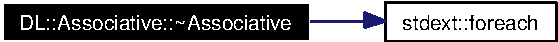
\includegraphics[width=151pt]{classDL_1_1Associative_a1_cgraph}
\end{center}
\end{figure}


\subsection{Member Function Documentation}
\hypertarget{classDL_1_1Associative_a3}{
\index{DL::Associative@{DL::Associative}!emit@{emit}}
\index{emit@{emit}!DL::Associative@{DL::Associative}}
\subsubsection[emit]{\setlength{\rightskip}{0pt plus 5cm}template$<$class Key\-Type, class Compare = std::less$<$Key\-Type$>$$>$ void \hyperlink{classDL_1_1Associative}{DL::Associative}$<$ Key\-Type, Compare $>$::emit (\hyperlink{classDL_1_1Associative_w1}{key\_\-type} {\em key})\hspace{0.3cm}{\tt  \mbox{[}inline\mbox{]}}}}
\label{classDL_1_1Associative_a3}




Definition at line 53 of file Associative.hpp.

References DL::Associative$<$ Key\-Type, Compare $>$::m\_\-data.

Referenced by main().\hypertarget{classDL_1_1Associative_a2}{
\index{DL::Associative@{DL::Associative}!insert@{insert}}
\index{insert@{insert}!DL::Associative@{DL::Associative}}
\subsubsection[insert]{\setlength{\rightskip}{0pt plus 5cm}template$<$class Key\-Type, class Compare = std::less$<$Key\-Type$>$$>$ void \hyperlink{classDL_1_1Associative}{DL::Associative}$<$ Key\-Type, Compare $>$::insert (\hyperlink{classDL_1_1Associative_w1}{key\_\-type} {\em key}, \hyperlink{namespaceDL_a0}{Delegate\-Obj} {\em Callback})\hspace{0.3cm}{\tt  \mbox{[}inline\mbox{]}}}}
\label{classDL_1_1Associative_a2}




Definition at line 49 of file Associative.hpp.

References DL::Associative$<$ Key\-Type, Compare $>$::m\_\-data.

Referenced by main().

\subsection{Member Data Documentation}
\hypertarget{classDL_1_1Associative_r0}{
\index{DL::Associative@{DL::Associative}!m_data@{m\_\-data}}
\index{m_data@{m\_\-data}!DL::Associative@{DL::Associative}}
\subsubsection[m\_\-data]{\setlength{\rightskip}{0pt plus 5cm}template$<$class Key\-Type, class Compare = std::less$<$Key\-Type$>$$>$ std::map$<$ \hyperlink{classDL_1_1Associative_w1}{key\_\-type} , \hyperlink{classDL_1_1DelegateBase}{Delegate\-Base}$\ast$ , \hyperlink{classDL_1_1Associative_w0}{compare\_\-type} $>$ \hyperlink{classDL_1_1Associative}{DL::Associative}$<$ Key\-Type, Compare $>$::\hyperlink{classDL_1_1Associative_r0}{m\_\-data}\hspace{0.3cm}{\tt  \mbox{[}private\mbox{]}}}}
\label{classDL_1_1Associative_r0}




Definition at line 60 of file Associative.hpp.

Referenced by DL::Associative$<$ Key\-Type, Compare $>$::emit(), DL::Associative$<$ Key\-Type, Compare $>$::insert(), and DL::Associative$<$ Key\-Type, Compare $>$::$\sim$Associative().

The documentation for this class was generated from the following file:\begin{CompactItemize}
\item 
/data/callbackext/Container/\hyperlink{Associative_8hpp}{Associative.hpp}\end{CompactItemize}

\hypertarget{classBlah}{
\section{Blah Class Reference}
\label{classBlah}\index{Blah@{Blah}}
}
\subsection*{Public Member Functions}
\begin{CompactItemize}
\item 
int \hyperlink{classBlah_a0}{Test\-AFunc} (int value)
\end{CompactItemize}


\subsection{Member Function Documentation}
\hypertarget{classBlah_a0}{
\index{Blah@{Blah}!TestAFunc@{TestAFunc}}
\index{TestAFunc@{TestAFunc}!Blah@{Blah}}
\subsubsection[TestAFunc]{\setlength{\rightskip}{0pt plus 5cm}int Blah::Test\-AFunc (int {\em value})\hspace{0.3cm}{\tt  \mbox{[}inline\mbox{]}}}}
\label{classBlah_a0}




Definition at line 33 of file Delegate\-Test1.cc.

The documentation for this class was generated from the following file:\begin{CompactItemize}
\item 
/data/callbackext/Tests/\hyperlink{DelegateTest1_8cc}{Delegate\-Test1.cc}\end{CompactItemize}

\hypertarget{classDL_1_1Delegate0}{
\section{DL::Delegate0$<$ Return\-Type, Class\-Type $>$ Class Template Reference}
\label{classDL_1_1Delegate0}\index{DL::Delegate0@{DL::Delegate0}}
}
{\tt \#include $<$Delegate0.hpp$>$}

Inherits \hyperlink{classDL_1_1DelegateBase}{DL::Delegate\-Base}.

Inheritance diagram for DL::Delegate0$<$ Return\-Type, Class\-Type $>$:\begin{figure}[H]
\begin{center}
\leavevmode
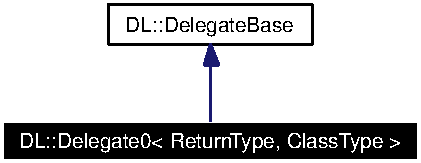
\includegraphics[width=118pt]{classDL_1_1Delegate0__inherit__graph}
\end{center}
\end{figure}
Collaboration diagram for DL::Delegate0$<$ Return\-Type, Class\-Type $>$:\begin{figure}[H]
\begin{center}
\leavevmode
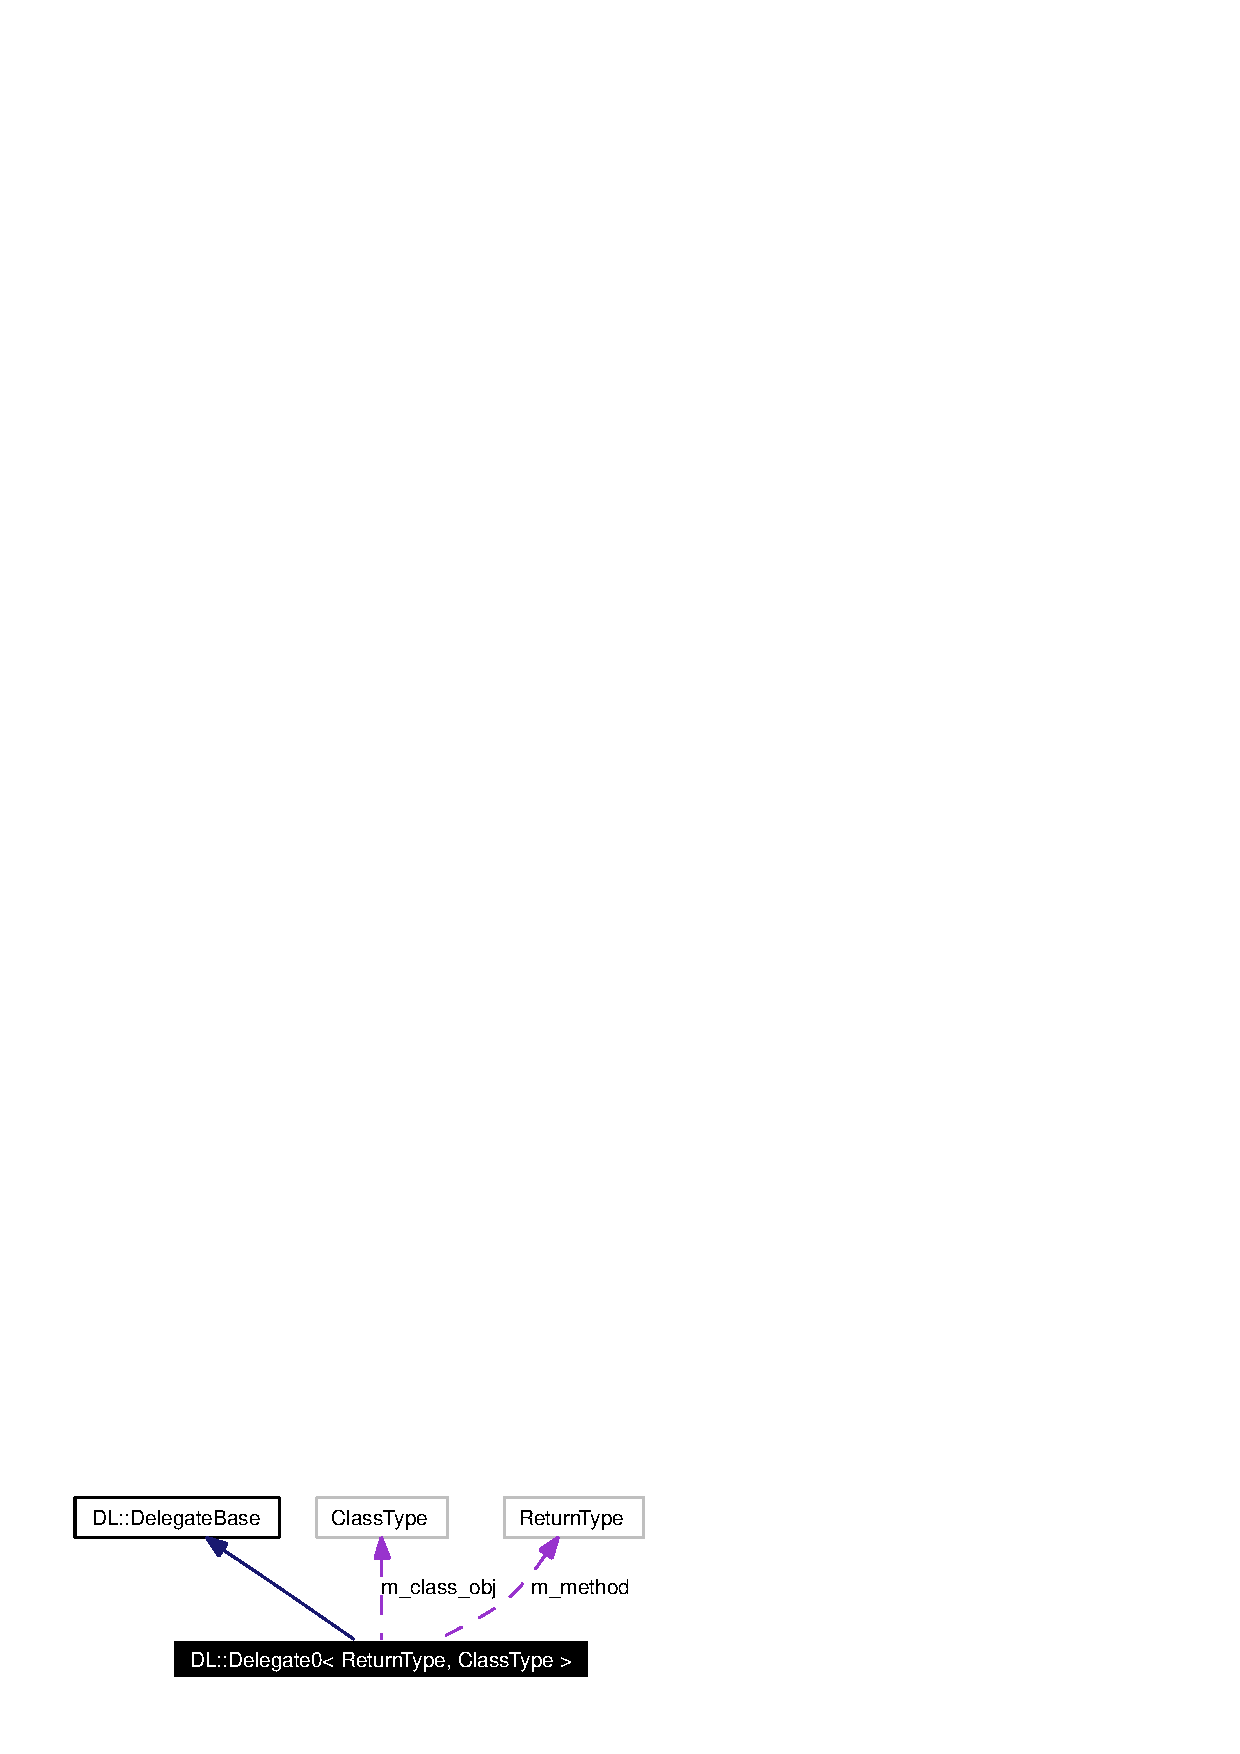
\includegraphics[width=162pt]{classDL_1_1Delegate0__coll__graph}
\end{center}
\end{figure}
\subsection*{Public Member Functions}
\begin{CompactItemize}
\item 
\hyperlink{classDL_1_1Delegate0_a0}{Delegate0} (Class\-Type $\ast$class\_\-obj, Return\-Type(Class\-Type::$\ast$method)())
\item 
virtual \hyperlink{classDL_1_1Delegate0_a1}{$\sim$Delegate0} ()
\item 
void \hyperlink{classDL_1_1Delegate0_a2}{Invoke} ()
\end{CompactItemize}
\subsection*{Private Member Functions}
\begin{CompactItemize}
\item 
\hyperlink{classDL_1_1Delegate0_d0}{Delegate0} ()
\end{CompactItemize}
\subsection*{Private Attributes}
\begin{CompactItemize}
\item 
Class\-Type $\ast$ \hyperlink{classDL_1_1Delegate0_r0}{m\_\-class\_\-obj}
\item 
Return\-Type(Class\-Type::$\ast$ \hyperlink{classDL_1_1Delegate0_r1}{m\_\-method} )()
\end{CompactItemize}
\subsubsection*{template$<$class Return\-Type, class Class\-Type$>$ class DL::Delegate0$<$ Return\-Type, Class\-Type $>$}



\subsection{Constructor \& Destructor Documentation}
\hypertarget{classDL_1_1Delegate0_d0}{
\index{DL::Delegate0@{DL::Delegate0}!Delegate0@{Delegate0}}
\index{Delegate0@{Delegate0}!DL::Delegate0@{DL::Delegate0}}
\subsubsection[Delegate0]{\setlength{\rightskip}{0pt plus 5cm}template$<$class Return\-Type, class Class\-Type$>$ \hyperlink{classDL_1_1Delegate0}{DL::Delegate0}$<$ Return\-Type, Class\-Type $>$::\hyperlink{classDL_1_1Delegate0}{Delegate0} ()\hspace{0.3cm}{\tt  \mbox{[}inline, private\mbox{]}}}}
\label{classDL_1_1Delegate0_d0}




Definition at line 31 of file Delegate0.hpp.\hypertarget{classDL_1_1Delegate0_a0}{
\index{DL::Delegate0@{DL::Delegate0}!Delegate0@{Delegate0}}
\index{Delegate0@{Delegate0}!DL::Delegate0@{DL::Delegate0}}
\subsubsection[Delegate0]{\setlength{\rightskip}{0pt plus 5cm}template$<$class Return\-Type, class Class\-Type$>$ \hyperlink{classDL_1_1Delegate0}{DL::Delegate0}$<$ Return\-Type, Class\-Type $>$::\hyperlink{classDL_1_1Delegate0}{Delegate0} (Class\-Type $\ast$ {\em class\_\-obj}, Return\-Type(Class\-Type::$\ast$)() {\em method})\hspace{0.3cm}{\tt  \mbox{[}inline\mbox{]}}}}
\label{classDL_1_1Delegate0_a0}




Definition at line 33 of file Delegate0.hpp.

References DL::Delegate0$<$ Return\-Type, Class\-Type $>$::m\_\-class\_\-obj, and DL::Delegate0$<$ Return\-Type, Class\-Type $>$::m\_\-method.\hypertarget{classDL_1_1Delegate0_a1}{
\index{DL::Delegate0@{DL::Delegate0}!~Delegate0@{$\sim$Delegate0}}
\index{~Delegate0@{$\sim$Delegate0}!DL::Delegate0@{DL::Delegate0}}
\subsubsection[$\sim$Delegate0]{\setlength{\rightskip}{0pt plus 5cm}template$<$class Return\-Type, class Class\-Type$>$ virtual \hyperlink{classDL_1_1Delegate0}{DL::Delegate0}$<$ Return\-Type, Class\-Type $>$::$\sim$\hyperlink{classDL_1_1Delegate0}{Delegate0} ()\hspace{0.3cm}{\tt  \mbox{[}inline, virtual\mbox{]}}}}
\label{classDL_1_1Delegate0_a1}




Definition at line 37 of file Delegate0.hpp.

\subsection{Member Function Documentation}
\hypertarget{classDL_1_1Delegate0_a2}{
\index{DL::Delegate0@{DL::Delegate0}!Invoke@{Invoke}}
\index{Invoke@{Invoke}!DL::Delegate0@{DL::Delegate0}}
\subsubsection[Invoke]{\setlength{\rightskip}{0pt plus 5cm}template$<$class Return\-Type, class Class\-Type$>$ void \hyperlink{classDL_1_1Delegate0}{DL::Delegate0}$<$ Return\-Type, Class\-Type $>$::Invoke ()\hspace{0.3cm}{\tt  \mbox{[}inline, virtual\mbox{]}}}}
\label{classDL_1_1Delegate0_a2}




Implements \hyperlink{classDL_1_1DelegateBase_a2}{DL::Delegate\-Base}.

Definition at line 38 of file Delegate0.hpp.

References DL::Delegate0$<$ Return\-Type, Class\-Type $>$::m\_\-class\_\-obj, and DL::Delegate0$<$ Return\-Type, Class\-Type $>$::m\_\-method.

\subsection{Member Data Documentation}
\hypertarget{classDL_1_1Delegate0_r0}{
\index{DL::Delegate0@{DL::Delegate0}!m_class_obj@{m\_\-class\_\-obj}}
\index{m_class_obj@{m\_\-class\_\-obj}!DL::Delegate0@{DL::Delegate0}}
\subsubsection[m\_\-class\_\-obj]{\setlength{\rightskip}{0pt plus 5cm}template$<$class Return\-Type, class Class\-Type$>$ Class\-Type$\ast$ \hyperlink{classDL_1_1Delegate0}{DL::Delegate0}$<$ Return\-Type, Class\-Type $>$::\hyperlink{classDL_1_1Delegate0_r0}{m\_\-class\_\-obj}\hspace{0.3cm}{\tt  \mbox{[}private\mbox{]}}}}
\label{classDL_1_1Delegate0_r0}




Definition at line 29 of file Delegate0.hpp.

Referenced by DL::Delegate0$<$ Return\-Type, Class\-Type $>$::Delegate0(), and DL::Delegate0$<$ Return\-Type, Class\-Type $>$::Invoke().\hypertarget{classDL_1_1Delegate0_r1}{
\index{DL::Delegate0@{DL::Delegate0}!m_method@{m\_\-method}}
\index{m_method@{m\_\-method}!DL::Delegate0@{DL::Delegate0}}
\subsubsection[m\_\-method]{\setlength{\rightskip}{0pt plus 5cm}template$<$class Return\-Type, class Class\-Type$>$ Return\-Type(Class\-Type::$\ast$ \hyperlink{classDL_1_1Delegate0}{DL::Delegate0}$<$ Return\-Type, Class\-Type $>$::\hyperlink{classDL_1_1Delegate0_r1}{m\_\-method})()\hspace{0.3cm}{\tt  \mbox{[}private\mbox{]}}}}
\label{classDL_1_1Delegate0_r1}




Referenced by DL::Delegate0$<$ Return\-Type, Class\-Type $>$::Delegate0(), and DL::Delegate0$<$ Return\-Type, Class\-Type $>$::Invoke().

The documentation for this class was generated from the following file:\begin{CompactItemize}
\item 
/data/callbackext/Delegate\-N/\hyperlink{Delegate0_8hpp}{Delegate0.hpp}\end{CompactItemize}

\hypertarget{classDL_1_1Delegate1}{
\section{DL::Delegate1$<$ Return\-Type, Class\-Type, Param1 $>$ Class Template Reference}
\label{classDL_1_1Delegate1}\index{DL::Delegate1@{DL::Delegate1}}
}
{\tt \#include $<$Delegate1.hpp$>$}

Inherits \hyperlink{classDL_1_1DelegateBase}{DL::Delegate\-Base}.

Inheritance diagram for DL::Delegate1$<$ Return\-Type, Class\-Type, Param1 $>$:\begin{figure}[H]
\begin{center}
\leavevmode
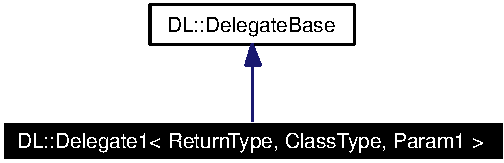
\includegraphics[width=138pt]{classDL_1_1Delegate1__inherit__graph}
\end{center}
\end{figure}
Collaboration diagram for DL::Delegate1$<$ Return\-Type, Class\-Type, Param1 $>$:\begin{figure}[H]
\begin{center}
\leavevmode
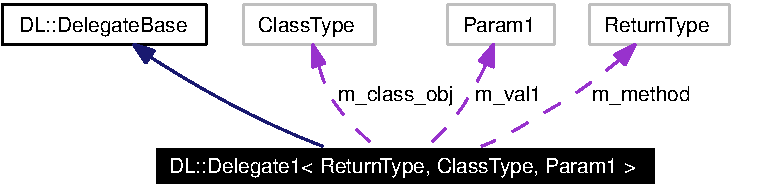
\includegraphics[width=200pt]{classDL_1_1Delegate1__coll__graph}
\end{center}
\end{figure}
\subsection*{Public Member Functions}
\begin{CompactItemize}
\item 
\hyperlink{classDL_1_1Delegate1_a0}{Delegate1} (Class\-Type $\ast$class\_\-obj, Return\-Type(Class\-Type::$\ast$method)(Param1), Param1 val1=Param1())
\item 
virtual \hyperlink{classDL_1_1Delegate1_a1}{$\sim$Delegate1} ()
\item 
void \hyperlink{classDL_1_1Delegate1_a2}{Invoke} ()
\item 
Return\-Type \hyperlink{classDL_1_1Delegate1_a3}{Invoke} (Param1 val1)
\end{CompactItemize}
\subsection*{Private Member Functions}
\begin{CompactItemize}
\item 
\hyperlink{classDL_1_1Delegate1_d0}{Delegate1} ()
\end{CompactItemize}
\subsection*{Private Attributes}
\begin{CompactItemize}
\item 
Class\-Type $\ast$ \hyperlink{classDL_1_1Delegate1_r0}{m\_\-class\_\-obj}
\item 
Return\-Type(Class\-Type::$\ast$ \hyperlink{classDL_1_1Delegate1_r1}{m\_\-method} )(Param1)
\item 
Param1 \hyperlink{classDL_1_1Delegate1_r2}{m\_\-val1}
\end{CompactItemize}


\subsection{Detailed Description}
\subsubsection*{template$<$class Return\-Type, class Class\-Type, class Param1$>$ class DL::Delegate1$<$ Return\-Type, Class\-Type, Param1 $>$}

Delegate for 1 Param



Definition at line 33 of file Delegate1.hpp.

\subsection{Constructor \& Destructor Documentation}
\hypertarget{classDL_1_1Delegate1_d0}{
\index{DL::Delegate1@{DL::Delegate1}!Delegate1@{Delegate1}}
\index{Delegate1@{Delegate1}!DL::Delegate1@{DL::Delegate1}}
\subsubsection[Delegate1]{\setlength{\rightskip}{0pt plus 5cm}template$<$class Return\-Type, class Class\-Type, class Param1$>$ \hyperlink{classDL_1_1Delegate1}{DL::Delegate1}$<$ Return\-Type, Class\-Type, Param1 $>$::\hyperlink{classDL_1_1Delegate1}{Delegate1} ()\hspace{0.3cm}{\tt  \mbox{[}inline, private\mbox{]}}}}
\label{classDL_1_1Delegate1_d0}




Definition at line 38 of file Delegate1.hpp.\hypertarget{classDL_1_1Delegate1_a0}{
\index{DL::Delegate1@{DL::Delegate1}!Delegate1@{Delegate1}}
\index{Delegate1@{Delegate1}!DL::Delegate1@{DL::Delegate1}}
\subsubsection[Delegate1]{\setlength{\rightskip}{0pt plus 5cm}template$<$class Return\-Type, class Class\-Type, class Param1$>$ \hyperlink{classDL_1_1Delegate1}{DL::Delegate1}$<$ Return\-Type, Class\-Type, Param1 $>$::\hyperlink{classDL_1_1Delegate1}{Delegate1} (Class\-Type $\ast$ {\em class\_\-obj}, Return\-Type(Class\-Type::$\ast$)(Param1) {\em method}, Param1 {\em val1} = {\tt Param1()})\hspace{0.3cm}{\tt  \mbox{[}inline\mbox{]}}}}
\label{classDL_1_1Delegate1_a0}




Definition at line 40 of file Delegate1.hpp.

References DL::Delegate1$<$ Return\-Type, Class\-Type, Param1 $>$::m\_\-class\_\-obj, DL::Delegate1$<$ Return\-Type, Class\-Type, Param1 $>$::m\_\-method, and DL::Delegate1$<$ Return\-Type, Class\-Type, Param1 $>$::m\_\-val1.\hypertarget{classDL_1_1Delegate1_a1}{
\index{DL::Delegate1@{DL::Delegate1}!~Delegate1@{$\sim$Delegate1}}
\index{~Delegate1@{$\sim$Delegate1}!DL::Delegate1@{DL::Delegate1}}
\subsubsection[$\sim$Delegate1]{\setlength{\rightskip}{0pt plus 5cm}template$<$class Return\-Type, class Class\-Type, class Param1$>$ virtual \hyperlink{classDL_1_1Delegate1}{DL::Delegate1}$<$ Return\-Type, Class\-Type, Param1 $>$::$\sim$\hyperlink{classDL_1_1Delegate1}{Delegate1} ()\hspace{0.3cm}{\tt  \mbox{[}inline, virtual\mbox{]}}}}
\label{classDL_1_1Delegate1_a1}




Definition at line 45 of file Delegate1.hpp.

\subsection{Member Function Documentation}
\hypertarget{classDL_1_1Delegate1_a3}{
\index{DL::Delegate1@{DL::Delegate1}!Invoke@{Invoke}}
\index{Invoke@{Invoke}!DL::Delegate1@{DL::Delegate1}}
\subsubsection[Invoke]{\setlength{\rightskip}{0pt plus 5cm}template$<$class Return\-Type, class Class\-Type, class Param1$>$ Return\-Type \hyperlink{classDL_1_1Delegate1}{DL::Delegate1}$<$ Return\-Type, Class\-Type, Param1 $>$::Invoke (Param1 {\em val1})\hspace{0.3cm}{\tt  \mbox{[}inline\mbox{]}}}}
\label{classDL_1_1Delegate1_a3}




Definition at line 50 of file Delegate1.hpp.

References DL::Delegate1$<$ Return\-Type, Class\-Type, Param1 $>$::m\_\-class\_\-obj, and DL::Delegate1$<$ Return\-Type, Class\-Type, Param1 $>$::m\_\-method.\hypertarget{classDL_1_1Delegate1_a2}{
\index{DL::Delegate1@{DL::Delegate1}!Invoke@{Invoke}}
\index{Invoke@{Invoke}!DL::Delegate1@{DL::Delegate1}}
\subsubsection[Invoke]{\setlength{\rightskip}{0pt plus 5cm}template$<$class Return\-Type, class Class\-Type, class Param1$>$ void \hyperlink{classDL_1_1Delegate1}{DL::Delegate1}$<$ Return\-Type, Class\-Type, Param1 $>$::Invoke ()\hspace{0.3cm}{\tt  \mbox{[}inline, virtual\mbox{]}}}}
\label{classDL_1_1Delegate1_a2}




Implements \hyperlink{classDL_1_1DelegateBase_a2}{DL::Delegate\-Base}.

Definition at line 46 of file Delegate1.hpp.

References DL::Delegate1$<$ Return\-Type, Class\-Type, Param1 $>$::m\_\-class\_\-obj, DL::Delegate1$<$ Return\-Type, Class\-Type, Param1 $>$::m\_\-method, and DL::Delegate1$<$ Return\-Type, Class\-Type, Param1 $>$::m\_\-val1.

\subsection{Member Data Documentation}
\hypertarget{classDL_1_1Delegate1_r0}{
\index{DL::Delegate1@{DL::Delegate1}!m_class_obj@{m\_\-class\_\-obj}}
\index{m_class_obj@{m\_\-class\_\-obj}!DL::Delegate1@{DL::Delegate1}}
\subsubsection[m\_\-class\_\-obj]{\setlength{\rightskip}{0pt plus 5cm}template$<$class Return\-Type, class Class\-Type, class Param1$>$ Class\-Type$\ast$ \hyperlink{classDL_1_1Delegate1}{DL::Delegate1}$<$ Return\-Type, Class\-Type, Param1 $>$::\hyperlink{classDL_1_1Delegate1_r0}{m\_\-class\_\-obj}\hspace{0.3cm}{\tt  \mbox{[}private\mbox{]}}}}
\label{classDL_1_1Delegate1_r0}




Definition at line 35 of file Delegate1.hpp.

Referenced by DL::Delegate1$<$ Return\-Type, Class\-Type, Param1 $>$::Delegate1(), and DL::Delegate1$<$ Return\-Type, Class\-Type, Param1 $>$::Invoke().\hypertarget{classDL_1_1Delegate1_r1}{
\index{DL::Delegate1@{DL::Delegate1}!m_method@{m\_\-method}}
\index{m_method@{m\_\-method}!DL::Delegate1@{DL::Delegate1}}
\subsubsection[m\_\-method]{\setlength{\rightskip}{0pt plus 5cm}template$<$class Return\-Type, class Class\-Type, class Param1$>$ Return\-Type(Class\-Type::$\ast$ \hyperlink{classDL_1_1Delegate1}{DL::Delegate1}$<$ Return\-Type, Class\-Type, Param1 $>$::\hyperlink{classDL_1_1Delegate1_r1}{m\_\-method})(Param1)\hspace{0.3cm}{\tt  \mbox{[}private\mbox{]}}}}
\label{classDL_1_1Delegate1_r1}




Referenced by DL::Delegate1$<$ Return\-Type, Class\-Type, Param1 $>$::Delegate1(), and DL::Delegate1$<$ Return\-Type, Class\-Type, Param1 $>$::Invoke().\hypertarget{classDL_1_1Delegate1_r2}{
\index{DL::Delegate1@{DL::Delegate1}!m_val1@{m\_\-val1}}
\index{m_val1@{m\_\-val1}!DL::Delegate1@{DL::Delegate1}}
\subsubsection[m\_\-val1]{\setlength{\rightskip}{0pt plus 5cm}template$<$class Return\-Type, class Class\-Type, class Param1$>$ Param1 \hyperlink{classDL_1_1Delegate1}{DL::Delegate1}$<$ Return\-Type, Class\-Type, Param1 $>$::\hyperlink{classDL_1_1Delegate1_r2}{m\_\-val1}\hspace{0.3cm}{\tt  \mbox{[}private\mbox{]}}}}
\label{classDL_1_1Delegate1_r2}




Definition at line 37 of file Delegate1.hpp.

Referenced by DL::Delegate1$<$ Return\-Type, Class\-Type, Param1 $>$::Delegate1(), and DL::Delegate1$<$ Return\-Type, Class\-Type, Param1 $>$::Invoke().

The documentation for this class was generated from the following file:\begin{CompactItemize}
\item 
/data/callbackext/Delegate\-N/\hyperlink{Delegate1_8hpp}{Delegate1.hpp}\end{CompactItemize}

\hypertarget{classDL_1_1Delegate10}{
\section{DL::Delegate10$<$ Return\-Type, Class\-Type, Param1, Param2, Param3, Param4, Param5, Param6, Param7, Param8, Param9, Param10 $>$ Class Template Reference}
\label{classDL_1_1Delegate10}\index{DL::Delegate10@{DL::Delegate10}}
}
{\tt \#include $<$Delegate10.hpp$>$}

Inherits \hyperlink{classDL_1_1DelegateBase}{DL::Delegate\-Base}.

Inheritance diagram for DL::Delegate10$<$ Return\-Type, Class\-Type, Param1, Param2, Param3, Param4, Param5, Param6, Param7, Param8, Param9, Param10 $>$:\begin{figure}[H]
\begin{center}
\leavevmode
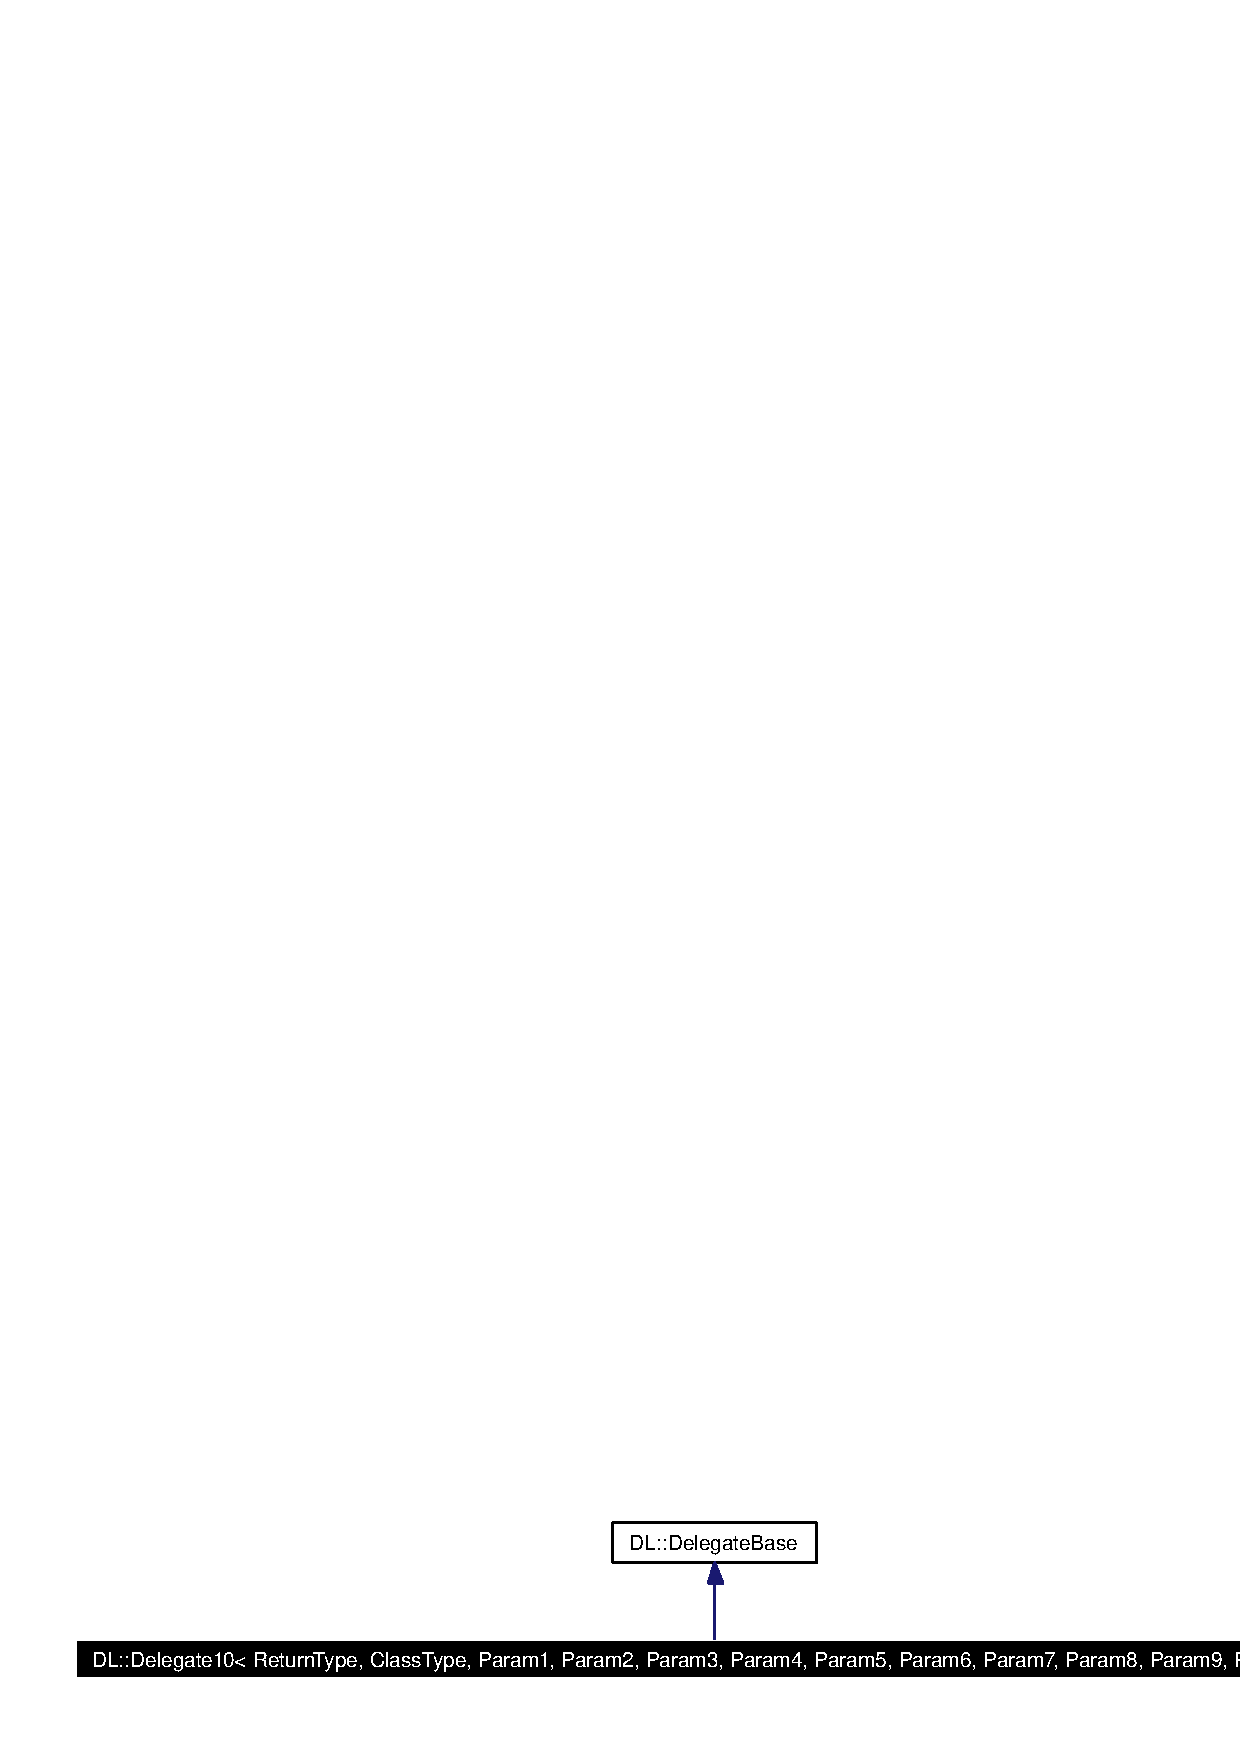
\includegraphics[width=325pt]{classDL_1_1Delegate10__inherit__graph}
\end{center}
\end{figure}
Collaboration diagram for DL::Delegate10$<$ Return\-Type, Class\-Type, Param1, Param2, Param3, Param4, Param5, Param6, Param7, Param8, Param9, Param10 $>$:\begin{figure}[H]
\begin{center}
\leavevmode
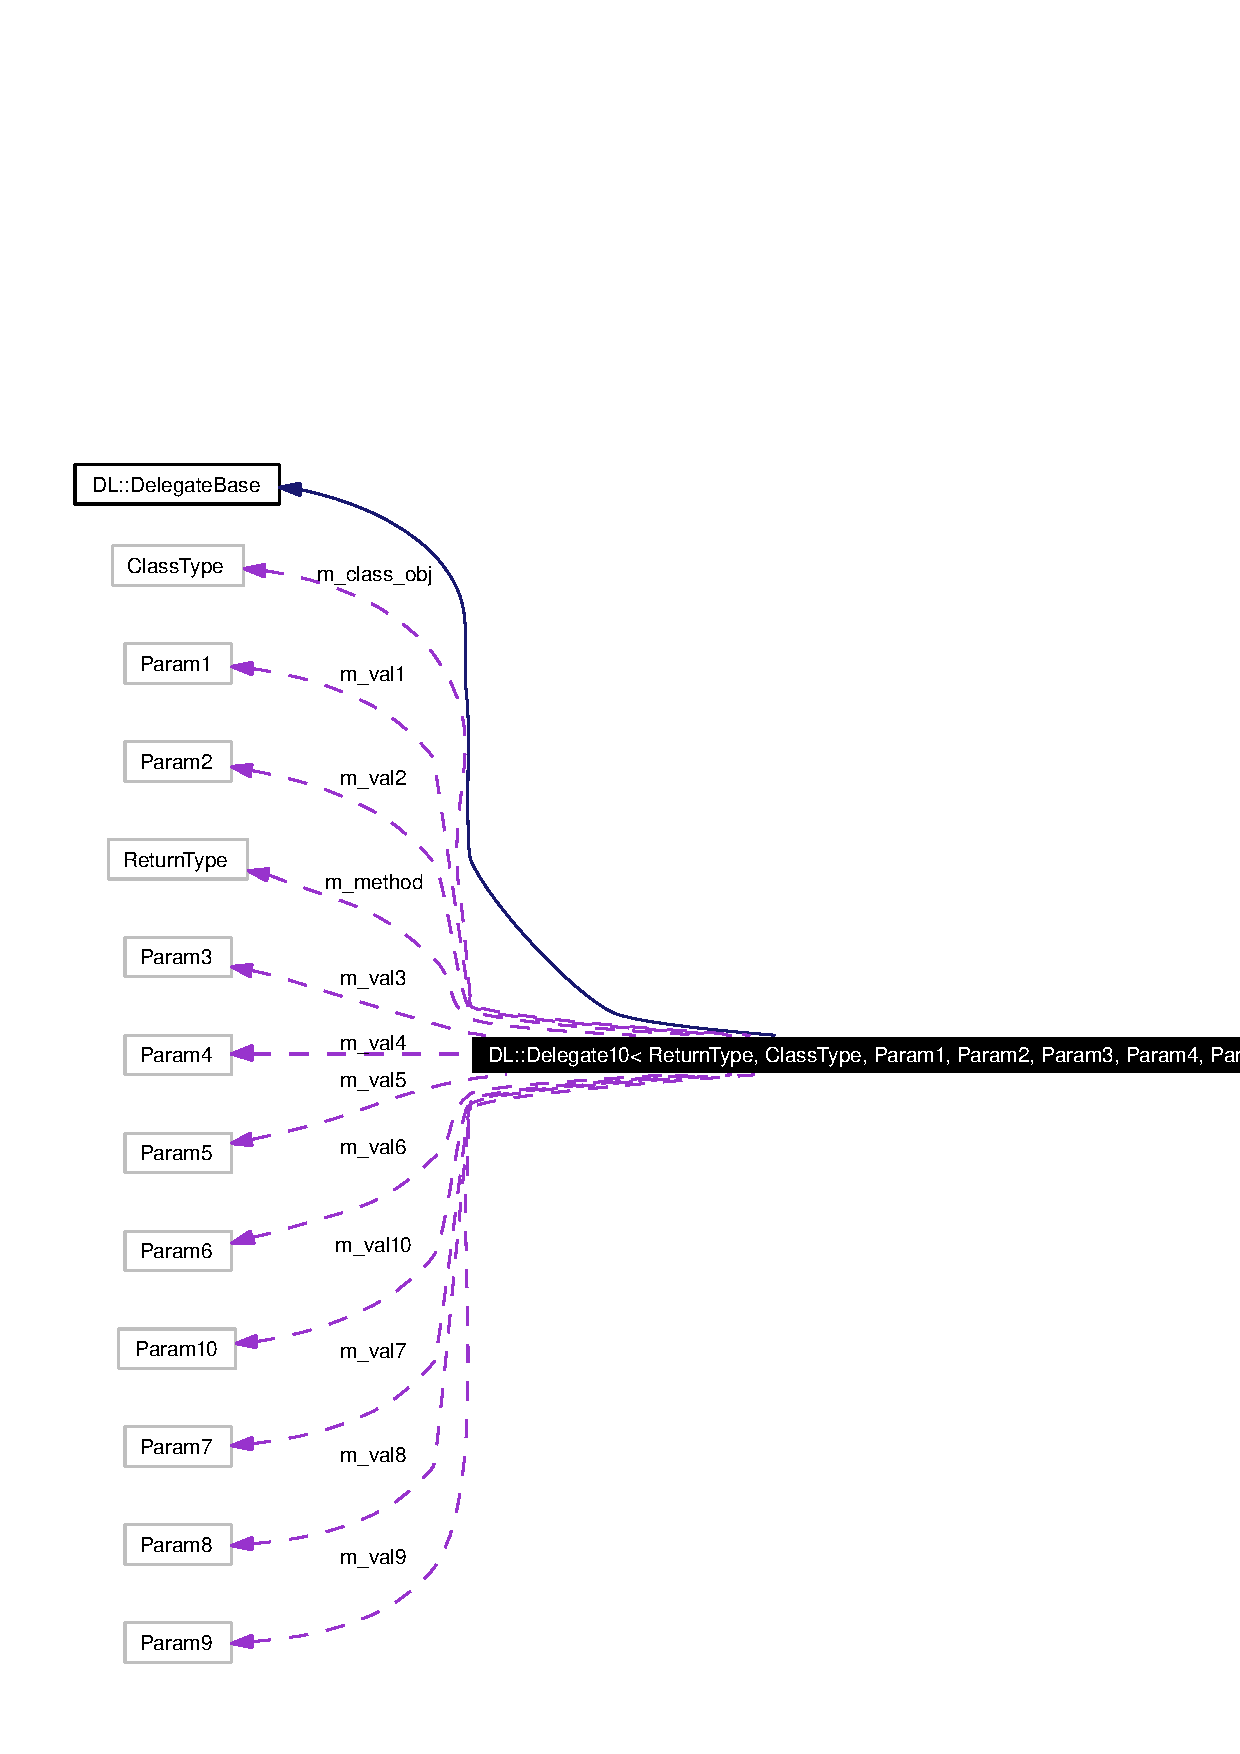
\includegraphics[width=420pt]{classDL_1_1Delegate10__coll__graph}
\end{center}
\end{figure}
\subsection*{Public Member Functions}
\begin{CompactItemize}
\item 
\hyperlink{classDL_1_1Delegate10_a0}{Delegate10} (Class\-Type $\ast$class\_\-obj, Return\-Type(Class\-Type::$\ast$method)(Param1, Param2, Param3, Param4, Param5, Param6, Param7, Param8, Param9, Param10), Param1 val1=Param1(), Param2 val2=Param2(), Param3 val3=Param3(), Param4 val4=Param4(), Param5 val5=Param5(), Param6 val6=Param6(), Param7 val7=Param7(), Param8 val8=Param8(), Param9 val9=Param9(), Param10 val10=Param10())
\item 
virtual \hyperlink{classDL_1_1Delegate10_a1}{$\sim$Delegate10} ()
\item 
void \hyperlink{classDL_1_1Delegate10_a2}{Invoke} ()
\item 
void \hyperlink{classDL_1_1Delegate10_a3}{Invoke} (Param1 val1, Param2 val2, Param3 val3, Param4 val4, Param5 val5, Param6 val6, Param7 val7, Param8 val8, Param9 val9, Param10 val10)
\end{CompactItemize}
\subsection*{Private Member Functions}
\begin{CompactItemize}
\item 
\hyperlink{classDL_1_1Delegate10_d0}{Delegate10} ()
\end{CompactItemize}
\subsection*{Private Attributes}
\begin{CompactItemize}
\item 
Class\-Type $\ast$ \hyperlink{classDL_1_1Delegate10_r0}{m\_\-class\_\-obj}
\item 
Return\-Type(Class\-Type::$\ast$ \hyperlink{classDL_1_1Delegate10_r1}{m\_\-method} )(Param1, Param2, Param3, Param4, Param5, Param6, Param7, Param8, Param9, Param10)
\item 
Param1 \hyperlink{classDL_1_1Delegate10_r2}{m\_\-val1}
\item 
Param2 \hyperlink{classDL_1_1Delegate10_r3}{m\_\-val2}
\item 
Param3 \hyperlink{classDL_1_1Delegate10_r4}{m\_\-val3}
\item 
Param4 \hyperlink{classDL_1_1Delegate10_r5}{m\_\-val4}
\item 
Param5 \hyperlink{classDL_1_1Delegate10_r6}{m\_\-val5}
\item 
Param6 \hyperlink{classDL_1_1Delegate10_r7}{m\_\-val6}
\item 
Param7 \hyperlink{classDL_1_1Delegate10_r8}{m\_\-val7}
\item 
Param8 \hyperlink{classDL_1_1Delegate10_r9}{m\_\-val8}
\item 
Param9 \hyperlink{classDL_1_1Delegate10_r10}{m\_\-val9}
\item 
Param10 \hyperlink{classDL_1_1Delegate10_r11}{m\_\-val10}
\end{CompactItemize}


\subsection{Detailed Description}
\subsubsection*{template$<$class Return\-Type, class Class\-Type, class Param1, class Param2, class Param3, class Param4, class Param5, class Param6, class Param7, class Param8, class Param9, class Param10$>$ class DL::Delegate10$<$ Return\-Type, Class\-Type, Param1, Param2, Param3, Param4, Param5, Param6, Param7, Param8, Param9, Param10 $>$}

Delegate for 10 Param



Definition at line 41 of file Delegate10.hpp.

\subsection{Constructor \& Destructor Documentation}
\hypertarget{classDL_1_1Delegate10_d0}{
\index{DL::Delegate10@{DL::Delegate10}!Delegate10@{Delegate10}}
\index{Delegate10@{Delegate10}!DL::Delegate10@{DL::Delegate10}}
\subsubsection[Delegate10]{\setlength{\rightskip}{0pt plus 5cm}template$<$class Return\-Type, class Class\-Type, class Param1, class Param2, class Param3, class Param4, class Param5, class Param6, class Param7, class Param8, class Param9, class Param10$>$ \hyperlink{classDL_1_1Delegate10}{DL::Delegate10}$<$ Return\-Type, Class\-Type, Param1, Param2, Param3, Param4, Param5, Param6, Param7, Param8, Param9, Param10 $>$::\hyperlink{classDL_1_1Delegate10}{Delegate10} ()\hspace{0.3cm}{\tt  \mbox{[}inline, private\mbox{]}}}}
\label{classDL_1_1Delegate10_d0}




Definition at line 55 of file Delegate10.hpp.\hypertarget{classDL_1_1Delegate10_a0}{
\index{DL::Delegate10@{DL::Delegate10}!Delegate10@{Delegate10}}
\index{Delegate10@{Delegate10}!DL::Delegate10@{DL::Delegate10}}
\subsubsection[Delegate10]{\setlength{\rightskip}{0pt plus 5cm}template$<$class Return\-Type, class Class\-Type, class Param1, class Param2, class Param3, class Param4, class Param5, class Param6, class Param7, class Param8, class Param9, class Param10$>$ \hyperlink{classDL_1_1Delegate10}{DL::Delegate10}$<$ Return\-Type, Class\-Type, Param1, Param2, Param3, Param4, Param5, Param6, Param7, Param8, Param9, Param10 $>$::\hyperlink{classDL_1_1Delegate10}{Delegate10} (Class\-Type $\ast$ {\em class\_\-obj}, Return\-Type(Class\-Type::$\ast$)(Param1, Param2, Param3, Param4, Param5, Param6, Param7, Param8, Param9, Param10) {\em method}, Param1 {\em val1} = {\tt Param1()}, Param2 {\em val2} = {\tt Param2()}, Param3 {\em val3} = {\tt Param3()}, Param4 {\em val4} = {\tt Param4()}, Param5 {\em val5} = {\tt Param5()}, Param6 {\em val6} = {\tt Param6()}, Param7 {\em val7} = {\tt Param7()}, Param8 {\em val8} = {\tt Param8()}, Param9 {\em val9} = {\tt Param9()}, Param10 {\em val10} = {\tt Param10()})\hspace{0.3cm}{\tt  \mbox{[}inline\mbox{]}}}}
\label{classDL_1_1Delegate10_a0}




Definition at line 57 of file Delegate10.hpp.

References DL::Delegate10$<$ Return\-Type, Class\-Type, Param1, Param2, Param3, Param4, Param5, Param6, Param7, Param8, Param9, Param10 $>$::m\_\-class\_\-obj, DL::Delegate10$<$ Return\-Type, Class\-Type, Param1, Param2, Param3, Param4, Param5, Param6, Param7, Param8, Param9, Param10 $>$::m\_\-method, DL::Delegate10$<$ Return\-Type, Class\-Type, Param1, Param2, Param3, Param4, Param5, Param6, Param7, Param8, Param9, Param10 $>$::m\_\-val1, DL::Delegate10$<$ Return\-Type, Class\-Type, Param1, Param2, Param3, Param4, Param5, Param6, Param7, Param8, Param9, Param10 $>$::m\_\-val10, DL::Delegate10$<$ Return\-Type, Class\-Type, Param1, Param2, Param3, Param4, Param5, Param6, Param7, Param8, Param9, Param10 $>$::m\_\-val2, DL::Delegate10$<$ Return\-Type, Class\-Type, Param1, Param2, Param3, Param4, Param5, Param6, Param7, Param8, Param9, Param10 $>$::m\_\-val3, DL::Delegate10$<$ Return\-Type, Class\-Type, Param1, Param2, Param3, Param4, Param5, Param6, Param7, Param8, Param9, Param10 $>$::m\_\-val4, DL::Delegate10$<$ Return\-Type, Class\-Type, Param1, Param2, Param3, Param4, Param5, Param6, Param7, Param8, Param9, Param10 $>$::m\_\-val5, DL::Delegate10$<$ Return\-Type, Class\-Type, Param1, Param2, Param3, Param4, Param5, Param6, Param7, Param8, Param9, Param10 $>$::m\_\-val6, DL::Delegate10$<$ Return\-Type, Class\-Type, Param1, Param2, Param3, Param4, Param5, Param6, Param7, Param8, Param9, Param10 $>$::m\_\-val7, DL::Delegate10$<$ Return\-Type, Class\-Type, Param1, Param2, Param3, Param4, Param5, Param6, Param7, Param8, Param9, Param10 $>$::m\_\-val8, and DL::Delegate10$<$ Return\-Type, Class\-Type, Param1, Param2, Param3, Param4, Param5, Param6, Param7, Param8, Param9, Param10 $>$::m\_\-val9.\hypertarget{classDL_1_1Delegate10_a1}{
\index{DL::Delegate10@{DL::Delegate10}!~Delegate10@{$\sim$Delegate10}}
\index{~Delegate10@{$\sim$Delegate10}!DL::Delegate10@{DL::Delegate10}}
\subsubsection[$\sim$Delegate10]{\setlength{\rightskip}{0pt plus 5cm}template$<$class Return\-Type, class Class\-Type, class Param1, class Param2, class Param3, class Param4, class Param5, class Param6, class Param7, class Param8, class Param9, class Param10$>$ virtual \hyperlink{classDL_1_1Delegate10}{DL::Delegate10}$<$ Return\-Type, Class\-Type, Param1, Param2, Param3, Param4, Param5, Param6, Param7, Param8, Param9, Param10 $>$::$\sim$\hyperlink{classDL_1_1Delegate10}{Delegate10} ()\hspace{0.3cm}{\tt  \mbox{[}inline, virtual\mbox{]}}}}
\label{classDL_1_1Delegate10_a1}




Definition at line 75 of file Delegate10.hpp.

\subsection{Member Function Documentation}
\hypertarget{classDL_1_1Delegate10_a3}{
\index{DL::Delegate10@{DL::Delegate10}!Invoke@{Invoke}}
\index{Invoke@{Invoke}!DL::Delegate10@{DL::Delegate10}}
\subsubsection[Invoke]{\setlength{\rightskip}{0pt plus 5cm}template$<$class Return\-Type, class Class\-Type, class Param1, class Param2, class Param3, class Param4, class Param5, class Param6, class Param7, class Param8, class Param9, class Param10$>$ void \hyperlink{classDL_1_1Delegate10}{DL::Delegate10}$<$ Return\-Type, Class\-Type, Param1, Param2, Param3, Param4, Param5, Param6, Param7, Param8, Param9, Param10 $>$::Invoke (Param1 {\em val1}, Param2 {\em val2}, Param3 {\em val3}, Param4 {\em val4}, Param5 {\em val5}, Param6 {\em val6}, Param7 {\em val7}, Param8 {\em val8}, Param9 {\em val9}, Param10 {\em val10})\hspace{0.3cm}{\tt  \mbox{[}inline\mbox{]}}}}
\label{classDL_1_1Delegate10_a3}




Definition at line 80 of file Delegate10.hpp.

References DL::Delegate10$<$ Return\-Type, Class\-Type, Param1, Param2, Param3, Param4, Param5, Param6, Param7, Param8, Param9, Param10 $>$::m\_\-class\_\-obj, and DL::Delegate10$<$ Return\-Type, Class\-Type, Param1, Param2, Param3, Param4, Param5, Param6, Param7, Param8, Param9, Param10 $>$::m\_\-method.\hypertarget{classDL_1_1Delegate10_a2}{
\index{DL::Delegate10@{DL::Delegate10}!Invoke@{Invoke}}
\index{Invoke@{Invoke}!DL::Delegate10@{DL::Delegate10}}
\subsubsection[Invoke]{\setlength{\rightskip}{0pt plus 5cm}template$<$class Return\-Type, class Class\-Type, class Param1, class Param2, class Param3, class Param4, class Param5, class Param6, class Param7, class Param8, class Param9, class Param10$>$ void \hyperlink{classDL_1_1Delegate10}{DL::Delegate10}$<$ Return\-Type, Class\-Type, Param1, Param2, Param3, Param4, Param5, Param6, Param7, Param8, Param9, Param10 $>$::Invoke ()\hspace{0.3cm}{\tt  \mbox{[}inline, virtual\mbox{]}}}}
\label{classDL_1_1Delegate10_a2}




Implements \hyperlink{classDL_1_1DelegateBase_a2}{DL::Delegate\-Base}.

Definition at line 76 of file Delegate10.hpp.

References DL::Delegate10$<$ Return\-Type, Class\-Type, Param1, Param2, Param3, Param4, Param5, Param6, Param7, Param8, Param9, Param10 $>$::m\_\-class\_\-obj, DL::Delegate10$<$ Return\-Type, Class\-Type, Param1, Param2, Param3, Param4, Param5, Param6, Param7, Param8, Param9, Param10 $>$::m\_\-method, DL::Delegate10$<$ Return\-Type, Class\-Type, Param1, Param2, Param3, Param4, Param5, Param6, Param7, Param8, Param9, Param10 $>$::m\_\-val1, DL::Delegate10$<$ Return\-Type, Class\-Type, Param1, Param2, Param3, Param4, Param5, Param6, Param7, Param8, Param9, Param10 $>$::m\_\-val10, DL::Delegate10$<$ Return\-Type, Class\-Type, Param1, Param2, Param3, Param4, Param5, Param6, Param7, Param8, Param9, Param10 $>$::m\_\-val2, DL::Delegate10$<$ Return\-Type, Class\-Type, Param1, Param2, Param3, Param4, Param5, Param6, Param7, Param8, Param9, Param10 $>$::m\_\-val3, DL::Delegate10$<$ Return\-Type, Class\-Type, Param1, Param2, Param3, Param4, Param5, Param6, Param7, Param8, Param9, Param10 $>$::m\_\-val4, DL::Delegate10$<$ Return\-Type, Class\-Type, Param1, Param2, Param3, Param4, Param5, Param6, Param7, Param8, Param9, Param10 $>$::m\_\-val5, DL::Delegate10$<$ Return\-Type, Class\-Type, Param1, Param2, Param3, Param4, Param5, Param6, Param7, Param8, Param9, Param10 $>$::m\_\-val6, DL::Delegate10$<$ Return\-Type, Class\-Type, Param1, Param2, Param3, Param4, Param5, Param6, Param7, Param8, Param9, Param10 $>$::m\_\-val7, DL::Delegate10$<$ Return\-Type, Class\-Type, Param1, Param2, Param3, Param4, Param5, Param6, Param7, Param8, Param9, Param10 $>$::m\_\-val8, and DL::Delegate10$<$ Return\-Type, Class\-Type, Param1, Param2, Param3, Param4, Param5, Param6, Param7, Param8, Param9, Param10 $>$::m\_\-val9.

\subsection{Member Data Documentation}
\hypertarget{classDL_1_1Delegate10_r0}{
\index{DL::Delegate10@{DL::Delegate10}!m_class_obj@{m\_\-class\_\-obj}}
\index{m_class_obj@{m\_\-class\_\-obj}!DL::Delegate10@{DL::Delegate10}}
\subsubsection[m\_\-class\_\-obj]{\setlength{\rightskip}{0pt plus 5cm}template$<$class Return\-Type, class Class\-Type, class Param1, class Param2, class Param3, class Param4, class Param5, class Param6, class Param7, class Param8, class Param9, class Param10$>$ Class\-Type$\ast$ \hyperlink{classDL_1_1Delegate10}{DL::Delegate10}$<$ Return\-Type, Class\-Type, Param1, Param2, Param3, Param4, Param5, Param6, Param7, Param8, Param9, Param10 $>$::\hyperlink{classDL_1_1Delegate10_r0}{m\_\-class\_\-obj}\hspace{0.3cm}{\tt  \mbox{[}private\mbox{]}}}}
\label{classDL_1_1Delegate10_r0}




Definition at line 43 of file Delegate10.hpp.

Referenced by DL::Delegate10$<$ Return\-Type, Class\-Type, Param1, Param2, Param3, Param4, Param5, Param6, Param7, Param8, Param9, Param10 $>$::Delegate10(), and DL::Delegate10$<$ Return\-Type, Class\-Type, Param1, Param2, Param3, Param4, Param5, Param6, Param7, Param8, Param9, Param10 $>$::Invoke().\hypertarget{classDL_1_1Delegate10_r1}{
\index{DL::Delegate10@{DL::Delegate10}!m_method@{m\_\-method}}
\index{m_method@{m\_\-method}!DL::Delegate10@{DL::Delegate10}}
\subsubsection[m\_\-method]{\setlength{\rightskip}{0pt plus 5cm}template$<$class Return\-Type, class Class\-Type, class Param1, class Param2, class Param3, class Param4, class Param5, class Param6, class Param7, class Param8, class Param9, class Param10$>$ Return\-Type(Class\-Type::$\ast$ \hyperlink{classDL_1_1Delegate10}{DL::Delegate10}$<$ Return\-Type, Class\-Type, Param1, Param2, Param3, Param4, Param5, Param6, Param7, Param8, Param9, Param10 $>$::\hyperlink{classDL_1_1Delegate10_r1}{m\_\-method})(Param1, Param2, Param3, Param4, Param5, Param6, Param7, Param8, Param9, Param10)\hspace{0.3cm}{\tt  \mbox{[}private\mbox{]}}}}
\label{classDL_1_1Delegate10_r1}




Referenced by DL::Delegate10$<$ Return\-Type, Class\-Type, Param1, Param2, Param3, Param4, Param5, Param6, Param7, Param8, Param9, Param10 $>$::Delegate10(), and DL::Delegate10$<$ Return\-Type, Class\-Type, Param1, Param2, Param3, Param4, Param5, Param6, Param7, Param8, Param9, Param10 $>$::Invoke().\hypertarget{classDL_1_1Delegate10_r2}{
\index{DL::Delegate10@{DL::Delegate10}!m_val1@{m\_\-val1}}
\index{m_val1@{m\_\-val1}!DL::Delegate10@{DL::Delegate10}}
\subsubsection[m\_\-val1]{\setlength{\rightskip}{0pt plus 5cm}template$<$class Return\-Type, class Class\-Type, class Param1, class Param2, class Param3, class Param4, class Param5, class Param6, class Param7, class Param8, class Param9, class Param10$>$ Param1 \hyperlink{classDL_1_1Delegate10}{DL::Delegate10}$<$ Return\-Type, Class\-Type, Param1, Param2, Param3, Param4, Param5, Param6, Param7, Param8, Param9, Param10 $>$::\hyperlink{classDL_1_1Delegate10_r2}{m\_\-val1}\hspace{0.3cm}{\tt  \mbox{[}private\mbox{]}}}}
\label{classDL_1_1Delegate10_r2}




Definition at line 45 of file Delegate10.hpp.

Referenced by DL::Delegate10$<$ Return\-Type, Class\-Type, Param1, Param2, Param3, Param4, Param5, Param6, Param7, Param8, Param9, Param10 $>$::Delegate10(), and DL::Delegate10$<$ Return\-Type, Class\-Type, Param1, Param2, Param3, Param4, Param5, Param6, Param7, Param8, Param9, Param10 $>$::Invoke().\hypertarget{classDL_1_1Delegate10_r11}{
\index{DL::Delegate10@{DL::Delegate10}!m_val10@{m\_\-val10}}
\index{m_val10@{m\_\-val10}!DL::Delegate10@{DL::Delegate10}}
\subsubsection[m\_\-val10]{\setlength{\rightskip}{0pt plus 5cm}template$<$class Return\-Type, class Class\-Type, class Param1, class Param2, class Param3, class Param4, class Param5, class Param6, class Param7, class Param8, class Param9, class Param10$>$ Param10 \hyperlink{classDL_1_1Delegate10}{DL::Delegate10}$<$ Return\-Type, Class\-Type, Param1, Param2, Param3, Param4, Param5, Param6, Param7, Param8, Param9, Param10 $>$::\hyperlink{classDL_1_1Delegate10_r11}{m\_\-val10}\hspace{0.3cm}{\tt  \mbox{[}private\mbox{]}}}}
\label{classDL_1_1Delegate10_r11}




Definition at line 54 of file Delegate10.hpp.

Referenced by DL::Delegate10$<$ Return\-Type, Class\-Type, Param1, Param2, Param3, Param4, Param5, Param6, Param7, Param8, Param9, Param10 $>$::Delegate10(), and DL::Delegate10$<$ Return\-Type, Class\-Type, Param1, Param2, Param3, Param4, Param5, Param6, Param7, Param8, Param9, Param10 $>$::Invoke().\hypertarget{classDL_1_1Delegate10_r3}{
\index{DL::Delegate10@{DL::Delegate10}!m_val2@{m\_\-val2}}
\index{m_val2@{m\_\-val2}!DL::Delegate10@{DL::Delegate10}}
\subsubsection[m\_\-val2]{\setlength{\rightskip}{0pt plus 5cm}template$<$class Return\-Type, class Class\-Type, class Param1, class Param2, class Param3, class Param4, class Param5, class Param6, class Param7, class Param8, class Param9, class Param10$>$ Param2 \hyperlink{classDL_1_1Delegate10}{DL::Delegate10}$<$ Return\-Type, Class\-Type, Param1, Param2, Param3, Param4, Param5, Param6, Param7, Param8, Param9, Param10 $>$::\hyperlink{classDL_1_1Delegate10_r3}{m\_\-val2}\hspace{0.3cm}{\tt  \mbox{[}private\mbox{]}}}}
\label{classDL_1_1Delegate10_r3}




Definition at line 46 of file Delegate10.hpp.

Referenced by DL::Delegate10$<$ Return\-Type, Class\-Type, Param1, Param2, Param3, Param4, Param5, Param6, Param7, Param8, Param9, Param10 $>$::Delegate10(), and DL::Delegate10$<$ Return\-Type, Class\-Type, Param1, Param2, Param3, Param4, Param5, Param6, Param7, Param8, Param9, Param10 $>$::Invoke().\hypertarget{classDL_1_1Delegate10_r4}{
\index{DL::Delegate10@{DL::Delegate10}!m_val3@{m\_\-val3}}
\index{m_val3@{m\_\-val3}!DL::Delegate10@{DL::Delegate10}}
\subsubsection[m\_\-val3]{\setlength{\rightskip}{0pt plus 5cm}template$<$class Return\-Type, class Class\-Type, class Param1, class Param2, class Param3, class Param4, class Param5, class Param6, class Param7, class Param8, class Param9, class Param10$>$ Param3 \hyperlink{classDL_1_1Delegate10}{DL::Delegate10}$<$ Return\-Type, Class\-Type, Param1, Param2, Param3, Param4, Param5, Param6, Param7, Param8, Param9, Param10 $>$::\hyperlink{classDL_1_1Delegate10_r4}{m\_\-val3}\hspace{0.3cm}{\tt  \mbox{[}private\mbox{]}}}}
\label{classDL_1_1Delegate10_r4}




Definition at line 47 of file Delegate10.hpp.

Referenced by DL::Delegate10$<$ Return\-Type, Class\-Type, Param1, Param2, Param3, Param4, Param5, Param6, Param7, Param8, Param9, Param10 $>$::Delegate10(), and DL::Delegate10$<$ Return\-Type, Class\-Type, Param1, Param2, Param3, Param4, Param5, Param6, Param7, Param8, Param9, Param10 $>$::Invoke().\hypertarget{classDL_1_1Delegate10_r5}{
\index{DL::Delegate10@{DL::Delegate10}!m_val4@{m\_\-val4}}
\index{m_val4@{m\_\-val4}!DL::Delegate10@{DL::Delegate10}}
\subsubsection[m\_\-val4]{\setlength{\rightskip}{0pt plus 5cm}template$<$class Return\-Type, class Class\-Type, class Param1, class Param2, class Param3, class Param4, class Param5, class Param6, class Param7, class Param8, class Param9, class Param10$>$ Param4 \hyperlink{classDL_1_1Delegate10}{DL::Delegate10}$<$ Return\-Type, Class\-Type, Param1, Param2, Param3, Param4, Param5, Param6, Param7, Param8, Param9, Param10 $>$::\hyperlink{classDL_1_1Delegate10_r5}{m\_\-val4}\hspace{0.3cm}{\tt  \mbox{[}private\mbox{]}}}}
\label{classDL_1_1Delegate10_r5}




Definition at line 48 of file Delegate10.hpp.

Referenced by DL::Delegate10$<$ Return\-Type, Class\-Type, Param1, Param2, Param3, Param4, Param5, Param6, Param7, Param8, Param9, Param10 $>$::Delegate10(), and DL::Delegate10$<$ Return\-Type, Class\-Type, Param1, Param2, Param3, Param4, Param5, Param6, Param7, Param8, Param9, Param10 $>$::Invoke().\hypertarget{classDL_1_1Delegate10_r6}{
\index{DL::Delegate10@{DL::Delegate10}!m_val5@{m\_\-val5}}
\index{m_val5@{m\_\-val5}!DL::Delegate10@{DL::Delegate10}}
\subsubsection[m\_\-val5]{\setlength{\rightskip}{0pt plus 5cm}template$<$class Return\-Type, class Class\-Type, class Param1, class Param2, class Param3, class Param4, class Param5, class Param6, class Param7, class Param8, class Param9, class Param10$>$ Param5 \hyperlink{classDL_1_1Delegate10}{DL::Delegate10}$<$ Return\-Type, Class\-Type, Param1, Param2, Param3, Param4, Param5, Param6, Param7, Param8, Param9, Param10 $>$::\hyperlink{classDL_1_1Delegate10_r6}{m\_\-val5}\hspace{0.3cm}{\tt  \mbox{[}private\mbox{]}}}}
\label{classDL_1_1Delegate10_r6}




Definition at line 49 of file Delegate10.hpp.

Referenced by DL::Delegate10$<$ Return\-Type, Class\-Type, Param1, Param2, Param3, Param4, Param5, Param6, Param7, Param8, Param9, Param10 $>$::Delegate10(), and DL::Delegate10$<$ Return\-Type, Class\-Type, Param1, Param2, Param3, Param4, Param5, Param6, Param7, Param8, Param9, Param10 $>$::Invoke().\hypertarget{classDL_1_1Delegate10_r7}{
\index{DL::Delegate10@{DL::Delegate10}!m_val6@{m\_\-val6}}
\index{m_val6@{m\_\-val6}!DL::Delegate10@{DL::Delegate10}}
\subsubsection[m\_\-val6]{\setlength{\rightskip}{0pt plus 5cm}template$<$class Return\-Type, class Class\-Type, class Param1, class Param2, class Param3, class Param4, class Param5, class Param6, class Param7, class Param8, class Param9, class Param10$>$ Param6 \hyperlink{classDL_1_1Delegate10}{DL::Delegate10}$<$ Return\-Type, Class\-Type, Param1, Param2, Param3, Param4, Param5, Param6, Param7, Param8, Param9, Param10 $>$::\hyperlink{classDL_1_1Delegate10_r7}{m\_\-val6}\hspace{0.3cm}{\tt  \mbox{[}private\mbox{]}}}}
\label{classDL_1_1Delegate10_r7}




Definition at line 50 of file Delegate10.hpp.

Referenced by DL::Delegate10$<$ Return\-Type, Class\-Type, Param1, Param2, Param3, Param4, Param5, Param6, Param7, Param8, Param9, Param10 $>$::Delegate10(), and DL::Delegate10$<$ Return\-Type, Class\-Type, Param1, Param2, Param3, Param4, Param5, Param6, Param7, Param8, Param9, Param10 $>$::Invoke().\hypertarget{classDL_1_1Delegate10_r8}{
\index{DL::Delegate10@{DL::Delegate10}!m_val7@{m\_\-val7}}
\index{m_val7@{m\_\-val7}!DL::Delegate10@{DL::Delegate10}}
\subsubsection[m\_\-val7]{\setlength{\rightskip}{0pt plus 5cm}template$<$class Return\-Type, class Class\-Type, class Param1, class Param2, class Param3, class Param4, class Param5, class Param6, class Param7, class Param8, class Param9, class Param10$>$ Param7 \hyperlink{classDL_1_1Delegate10}{DL::Delegate10}$<$ Return\-Type, Class\-Type, Param1, Param2, Param3, Param4, Param5, Param6, Param7, Param8, Param9, Param10 $>$::\hyperlink{classDL_1_1Delegate10_r8}{m\_\-val7}\hspace{0.3cm}{\tt  \mbox{[}private\mbox{]}}}}
\label{classDL_1_1Delegate10_r8}




Definition at line 51 of file Delegate10.hpp.

Referenced by DL::Delegate10$<$ Return\-Type, Class\-Type, Param1, Param2, Param3, Param4, Param5, Param6, Param7, Param8, Param9, Param10 $>$::Delegate10(), and DL::Delegate10$<$ Return\-Type, Class\-Type, Param1, Param2, Param3, Param4, Param5, Param6, Param7, Param8, Param9, Param10 $>$::Invoke().\hypertarget{classDL_1_1Delegate10_r9}{
\index{DL::Delegate10@{DL::Delegate10}!m_val8@{m\_\-val8}}
\index{m_val8@{m\_\-val8}!DL::Delegate10@{DL::Delegate10}}
\subsubsection[m\_\-val8]{\setlength{\rightskip}{0pt plus 5cm}template$<$class Return\-Type, class Class\-Type, class Param1, class Param2, class Param3, class Param4, class Param5, class Param6, class Param7, class Param8, class Param9, class Param10$>$ Param8 \hyperlink{classDL_1_1Delegate10}{DL::Delegate10}$<$ Return\-Type, Class\-Type, Param1, Param2, Param3, Param4, Param5, Param6, Param7, Param8, Param9, Param10 $>$::\hyperlink{classDL_1_1Delegate10_r9}{m\_\-val8}\hspace{0.3cm}{\tt  \mbox{[}private\mbox{]}}}}
\label{classDL_1_1Delegate10_r9}




Definition at line 52 of file Delegate10.hpp.

Referenced by DL::Delegate10$<$ Return\-Type, Class\-Type, Param1, Param2, Param3, Param4, Param5, Param6, Param7, Param8, Param9, Param10 $>$::Delegate10(), and DL::Delegate10$<$ Return\-Type, Class\-Type, Param1, Param2, Param3, Param4, Param5, Param6, Param7, Param8, Param9, Param10 $>$::Invoke().\hypertarget{classDL_1_1Delegate10_r10}{
\index{DL::Delegate10@{DL::Delegate10}!m_val9@{m\_\-val9}}
\index{m_val9@{m\_\-val9}!DL::Delegate10@{DL::Delegate10}}
\subsubsection[m\_\-val9]{\setlength{\rightskip}{0pt plus 5cm}template$<$class Return\-Type, class Class\-Type, class Param1, class Param2, class Param3, class Param4, class Param5, class Param6, class Param7, class Param8, class Param9, class Param10$>$ Param9 \hyperlink{classDL_1_1Delegate10}{DL::Delegate10}$<$ Return\-Type, Class\-Type, Param1, Param2, Param3, Param4, Param5, Param6, Param7, Param8, Param9, Param10 $>$::\hyperlink{classDL_1_1Delegate10_r10}{m\_\-val9}\hspace{0.3cm}{\tt  \mbox{[}private\mbox{]}}}}
\label{classDL_1_1Delegate10_r10}




Definition at line 53 of file Delegate10.hpp.

Referenced by DL::Delegate10$<$ Return\-Type, Class\-Type, Param1, Param2, Param3, Param4, Param5, Param6, Param7, Param8, Param9, Param10 $>$::Delegate10(), and DL::Delegate10$<$ Return\-Type, Class\-Type, Param1, Param2, Param3, Param4, Param5, Param6, Param7, Param8, Param9, Param10 $>$::Invoke().

The documentation for this class was generated from the following file:\begin{CompactItemize}
\item 
/data/callbackext/Delegate\-N/\hyperlink{Delegate10_8hpp}{Delegate10.hpp}\end{CompactItemize}

\hypertarget{classDL_1_1Delegate2}{
\section{DL::Delegate2$<$ Return\-Type, Class\-Type, Param1, Param2 $>$ Class Template Reference}
\label{classDL_1_1Delegate2}\index{DL::Delegate2@{DL::Delegate2}}
}
{\tt \#include $<$Delegate2.hpp$>$}

Inherits \hyperlink{classDL_1_1DelegateBase}{DL::Delegate\-Base}.

Inheritance diagram for DL::Delegate2$<$ Return\-Type, Class\-Type, Param1, Param2 $>$:\begin{figure}[H]
\begin{center}
\leavevmode
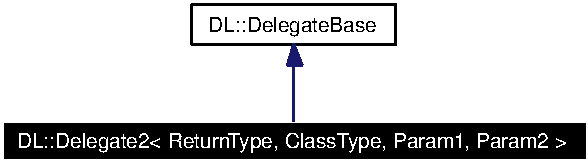
\includegraphics[width=158pt]{classDL_1_1Delegate2__inherit__graph}
\end{center}
\end{figure}
Collaboration diagram for DL::Delegate2$<$ Return\-Type, Class\-Type, Param1, Param2 $>$:\begin{figure}[H]
\begin{center}
\leavevmode
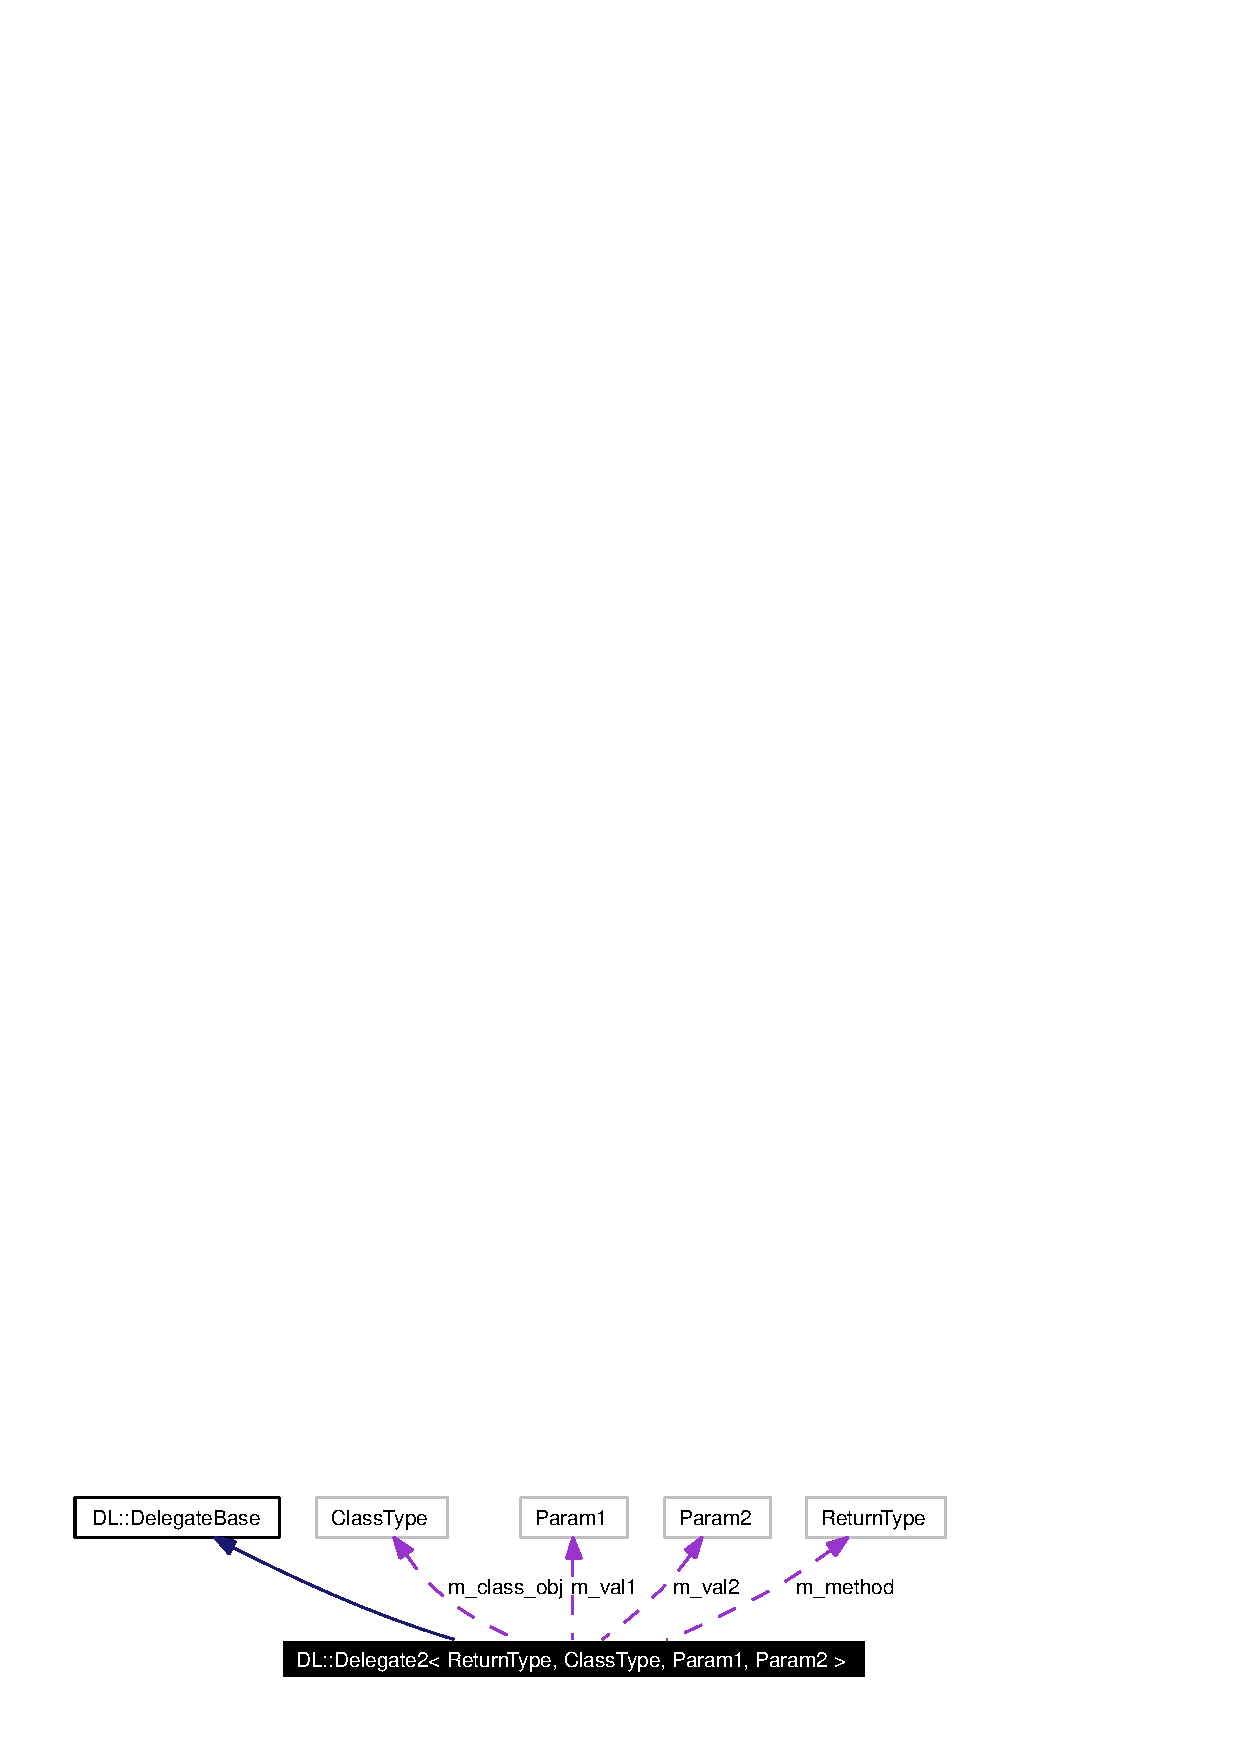
\includegraphics[width=234pt]{classDL_1_1Delegate2__coll__graph}
\end{center}
\end{figure}
\subsection*{Public Member Functions}
\begin{CompactItemize}
\item 
\hyperlink{classDL_1_1Delegate2_a0}{Delegate2} (Class\-Type $\ast$class\_\-obj, Return\-Type(Class\-Type::$\ast$method)(Param1, Param2), Param1 val1=Param1(), Param2 val2=Param2())
\item 
virtual \hyperlink{classDL_1_1Delegate2_a1}{$\sim$Delegate2} ()
\item 
void \hyperlink{classDL_1_1Delegate2_a2}{Invoke} ()
\item 
void \hyperlink{classDL_1_1Delegate2_a3}{Invoke} (Param1 val1, Param2 val2)
\end{CompactItemize}
\subsection*{Private Member Functions}
\begin{CompactItemize}
\item 
\hyperlink{classDL_1_1Delegate2_d0}{Delegate2} ()
\end{CompactItemize}
\subsection*{Private Attributes}
\begin{CompactItemize}
\item 
Class\-Type $\ast$ \hyperlink{classDL_1_1Delegate2_r0}{m\_\-class\_\-obj}
\item 
Return\-Type(Class\-Type::$\ast$ \hyperlink{classDL_1_1Delegate2_r1}{m\_\-method} )(Param1, Param2)
\item 
Param1 \hyperlink{classDL_1_1Delegate2_r2}{m\_\-val1}
\item 
Param2 \hyperlink{classDL_1_1Delegate2_r3}{m\_\-val2}
\end{CompactItemize}


\subsection{Detailed Description}
\subsubsection*{template$<$class Return\-Type, class Class\-Type, class Param1, class Param2$>$ class DL::Delegate2$<$ Return\-Type, Class\-Type, Param1, Param2 $>$}

Delegate for 2 Param



Definition at line 34 of file Delegate2.hpp.

\subsection{Constructor \& Destructor Documentation}
\hypertarget{classDL_1_1Delegate2_d0}{
\index{DL::Delegate2@{DL::Delegate2}!Delegate2@{Delegate2}}
\index{Delegate2@{Delegate2}!DL::Delegate2@{DL::Delegate2}}
\subsubsection[Delegate2]{\setlength{\rightskip}{0pt plus 5cm}template$<$class Return\-Type, class Class\-Type, class Param1, class Param2$>$ \hyperlink{classDL_1_1Delegate2}{DL::Delegate2}$<$ Return\-Type, Class\-Type, Param1, Param2 $>$::\hyperlink{classDL_1_1Delegate2}{Delegate2} ()\hspace{0.3cm}{\tt  \mbox{[}inline, private\mbox{]}}}}
\label{classDL_1_1Delegate2_d0}




Definition at line 40 of file Delegate2.hpp.\hypertarget{classDL_1_1Delegate2_a0}{
\index{DL::Delegate2@{DL::Delegate2}!Delegate2@{Delegate2}}
\index{Delegate2@{Delegate2}!DL::Delegate2@{DL::Delegate2}}
\subsubsection[Delegate2]{\setlength{\rightskip}{0pt plus 5cm}template$<$class Return\-Type, class Class\-Type, class Param1, class Param2$>$ \hyperlink{classDL_1_1Delegate2}{DL::Delegate2}$<$ Return\-Type, Class\-Type, Param1, Param2 $>$::\hyperlink{classDL_1_1Delegate2}{Delegate2} (Class\-Type $\ast$ {\em class\_\-obj}, Return\-Type(Class\-Type::$\ast$)(Param1, Param2) {\em method}, Param1 {\em val1} = {\tt Param1()}, Param2 {\em val2} = {\tt Param2()})\hspace{0.3cm}{\tt  \mbox{[}inline\mbox{]}}}}
\label{classDL_1_1Delegate2_a0}




Definition at line 42 of file Delegate2.hpp.

References DL::Delegate2$<$ Return\-Type, Class\-Type, Param1, Param2 $>$::m\_\-class\_\-obj, DL::Delegate2$<$ Return\-Type, Class\-Type, Param1, Param2 $>$::m\_\-method, DL::Delegate2$<$ Return\-Type, Class\-Type, Param1, Param2 $>$::m\_\-val1, and DL::Delegate2$<$ Return\-Type, Class\-Type, Param1, Param2 $>$::m\_\-val2.\hypertarget{classDL_1_1Delegate2_a1}{
\index{DL::Delegate2@{DL::Delegate2}!~Delegate2@{$\sim$Delegate2}}
\index{~Delegate2@{$\sim$Delegate2}!DL::Delegate2@{DL::Delegate2}}
\subsubsection[$\sim$Delegate2]{\setlength{\rightskip}{0pt plus 5cm}template$<$class Return\-Type, class Class\-Type, class Param1, class Param2$>$ virtual \hyperlink{classDL_1_1Delegate2}{DL::Delegate2}$<$ Return\-Type, Class\-Type, Param1, Param2 $>$::$\sim$\hyperlink{classDL_1_1Delegate2}{Delegate2} ()\hspace{0.3cm}{\tt  \mbox{[}inline, virtual\mbox{]}}}}
\label{classDL_1_1Delegate2_a1}




Definition at line 49 of file Delegate2.hpp.

\subsection{Member Function Documentation}
\hypertarget{classDL_1_1Delegate2_a3}{
\index{DL::Delegate2@{DL::Delegate2}!Invoke@{Invoke}}
\index{Invoke@{Invoke}!DL::Delegate2@{DL::Delegate2}}
\subsubsection[Invoke]{\setlength{\rightskip}{0pt plus 5cm}template$<$class Return\-Type, class Class\-Type, class Param1, class Param2$>$ void \hyperlink{classDL_1_1Delegate2}{DL::Delegate2}$<$ Return\-Type, Class\-Type, Param1, Param2 $>$::Invoke (Param1 {\em val1}, Param2 {\em val2})\hspace{0.3cm}{\tt  \mbox{[}inline\mbox{]}}}}
\label{classDL_1_1Delegate2_a3}




Definition at line 54 of file Delegate2.hpp.

References DL::Delegate2$<$ Return\-Type, Class\-Type, Param1, Param2 $>$::m\_\-class\_\-obj, and DL::Delegate2$<$ Return\-Type, Class\-Type, Param1, Param2 $>$::m\_\-method.\hypertarget{classDL_1_1Delegate2_a2}{
\index{DL::Delegate2@{DL::Delegate2}!Invoke@{Invoke}}
\index{Invoke@{Invoke}!DL::Delegate2@{DL::Delegate2}}
\subsubsection[Invoke]{\setlength{\rightskip}{0pt plus 5cm}template$<$class Return\-Type, class Class\-Type, class Param1, class Param2$>$ void \hyperlink{classDL_1_1Delegate2}{DL::Delegate2}$<$ Return\-Type, Class\-Type, Param1, Param2 $>$::Invoke ()\hspace{0.3cm}{\tt  \mbox{[}inline, virtual\mbox{]}}}}
\label{classDL_1_1Delegate2_a2}




Implements \hyperlink{classDL_1_1DelegateBase_a2}{DL::Delegate\-Base}.

Definition at line 50 of file Delegate2.hpp.

References DL::Delegate2$<$ Return\-Type, Class\-Type, Param1, Param2 $>$::m\_\-class\_\-obj, DL::Delegate2$<$ Return\-Type, Class\-Type, Param1, Param2 $>$::m\_\-method, DL::Delegate2$<$ Return\-Type, Class\-Type, Param1, Param2 $>$::m\_\-val1, and DL::Delegate2$<$ Return\-Type, Class\-Type, Param1, Param2 $>$::m\_\-val2.

\subsection{Member Data Documentation}
\hypertarget{classDL_1_1Delegate2_r0}{
\index{DL::Delegate2@{DL::Delegate2}!m_class_obj@{m\_\-class\_\-obj}}
\index{m_class_obj@{m\_\-class\_\-obj}!DL::Delegate2@{DL::Delegate2}}
\subsubsection[m\_\-class\_\-obj]{\setlength{\rightskip}{0pt plus 5cm}template$<$class Return\-Type, class Class\-Type, class Param1, class Param2$>$ Class\-Type$\ast$ \hyperlink{classDL_1_1Delegate2}{DL::Delegate2}$<$ Return\-Type, Class\-Type, Param1, Param2 $>$::\hyperlink{classDL_1_1Delegate2_r0}{m\_\-class\_\-obj}\hspace{0.3cm}{\tt  \mbox{[}private\mbox{]}}}}
\label{classDL_1_1Delegate2_r0}




Definition at line 36 of file Delegate2.hpp.

Referenced by DL::Delegate2$<$ Return\-Type, Class\-Type, Param1, Param2 $>$::Delegate2(), and DL::Delegate2$<$ Return\-Type, Class\-Type, Param1, Param2 $>$::Invoke().\hypertarget{classDL_1_1Delegate2_r1}{
\index{DL::Delegate2@{DL::Delegate2}!m_method@{m\_\-method}}
\index{m_method@{m\_\-method}!DL::Delegate2@{DL::Delegate2}}
\subsubsection[m\_\-method]{\setlength{\rightskip}{0pt plus 5cm}template$<$class Return\-Type, class Class\-Type, class Param1, class Param2$>$ Return\-Type(Class\-Type::$\ast$ \hyperlink{classDL_1_1Delegate2}{DL::Delegate2}$<$ Return\-Type, Class\-Type, Param1, Param2 $>$::\hyperlink{classDL_1_1Delegate2_r1}{m\_\-method})(Param1, Param2)\hspace{0.3cm}{\tt  \mbox{[}private\mbox{]}}}}
\label{classDL_1_1Delegate2_r1}




Referenced by DL::Delegate2$<$ Return\-Type, Class\-Type, Param1, Param2 $>$::Delegate2(), and DL::Delegate2$<$ Return\-Type, Class\-Type, Param1, Param2 $>$::Invoke().\hypertarget{classDL_1_1Delegate2_r2}{
\index{DL::Delegate2@{DL::Delegate2}!m_val1@{m\_\-val1}}
\index{m_val1@{m\_\-val1}!DL::Delegate2@{DL::Delegate2}}
\subsubsection[m\_\-val1]{\setlength{\rightskip}{0pt plus 5cm}template$<$class Return\-Type, class Class\-Type, class Param1, class Param2$>$ Param1 \hyperlink{classDL_1_1Delegate2}{DL::Delegate2}$<$ Return\-Type, Class\-Type, Param1, Param2 $>$::\hyperlink{classDL_1_1Delegate2_r2}{m\_\-val1}\hspace{0.3cm}{\tt  \mbox{[}private\mbox{]}}}}
\label{classDL_1_1Delegate2_r2}




Definition at line 38 of file Delegate2.hpp.

Referenced by DL::Delegate2$<$ Return\-Type, Class\-Type, Param1, Param2 $>$::Delegate2(), and DL::Delegate2$<$ Return\-Type, Class\-Type, Param1, Param2 $>$::Invoke().\hypertarget{classDL_1_1Delegate2_r3}{
\index{DL::Delegate2@{DL::Delegate2}!m_val2@{m\_\-val2}}
\index{m_val2@{m\_\-val2}!DL::Delegate2@{DL::Delegate2}}
\subsubsection[m\_\-val2]{\setlength{\rightskip}{0pt plus 5cm}template$<$class Return\-Type, class Class\-Type, class Param1, class Param2$>$ Param2 \hyperlink{classDL_1_1Delegate2}{DL::Delegate2}$<$ Return\-Type, Class\-Type, Param1, Param2 $>$::\hyperlink{classDL_1_1Delegate2_r3}{m\_\-val2}\hspace{0.3cm}{\tt  \mbox{[}private\mbox{]}}}}
\label{classDL_1_1Delegate2_r3}




Definition at line 39 of file Delegate2.hpp.

Referenced by DL::Delegate2$<$ Return\-Type, Class\-Type, Param1, Param2 $>$::Delegate2(), and DL::Delegate2$<$ Return\-Type, Class\-Type, Param1, Param2 $>$::Invoke().

The documentation for this class was generated from the following file:\begin{CompactItemize}
\item 
/data/callbackext/Delegate\-N/\hyperlink{Delegate2_8hpp}{Delegate2.hpp}\end{CompactItemize}

\hypertarget{classDL_1_1Delegate3}{
\section{DL::Delegate3$<$ Return\-Type, Class\-Type, Param1, Param2, Param3 $>$ Class Template Reference}
\label{classDL_1_1Delegate3}\index{DL::Delegate3@{DL::Delegate3}}
}
{\tt \#include $<$Delegate3.hpp$>$}

Inherits \hyperlink{classDL_1_1DelegateBase}{DL::Delegate\-Base}.

Inheritance diagram for DL::Delegate3$<$ Return\-Type, Class\-Type, Param1, Param2, Param3 $>$:\begin{figure}[H]
\begin{center}
\leavevmode
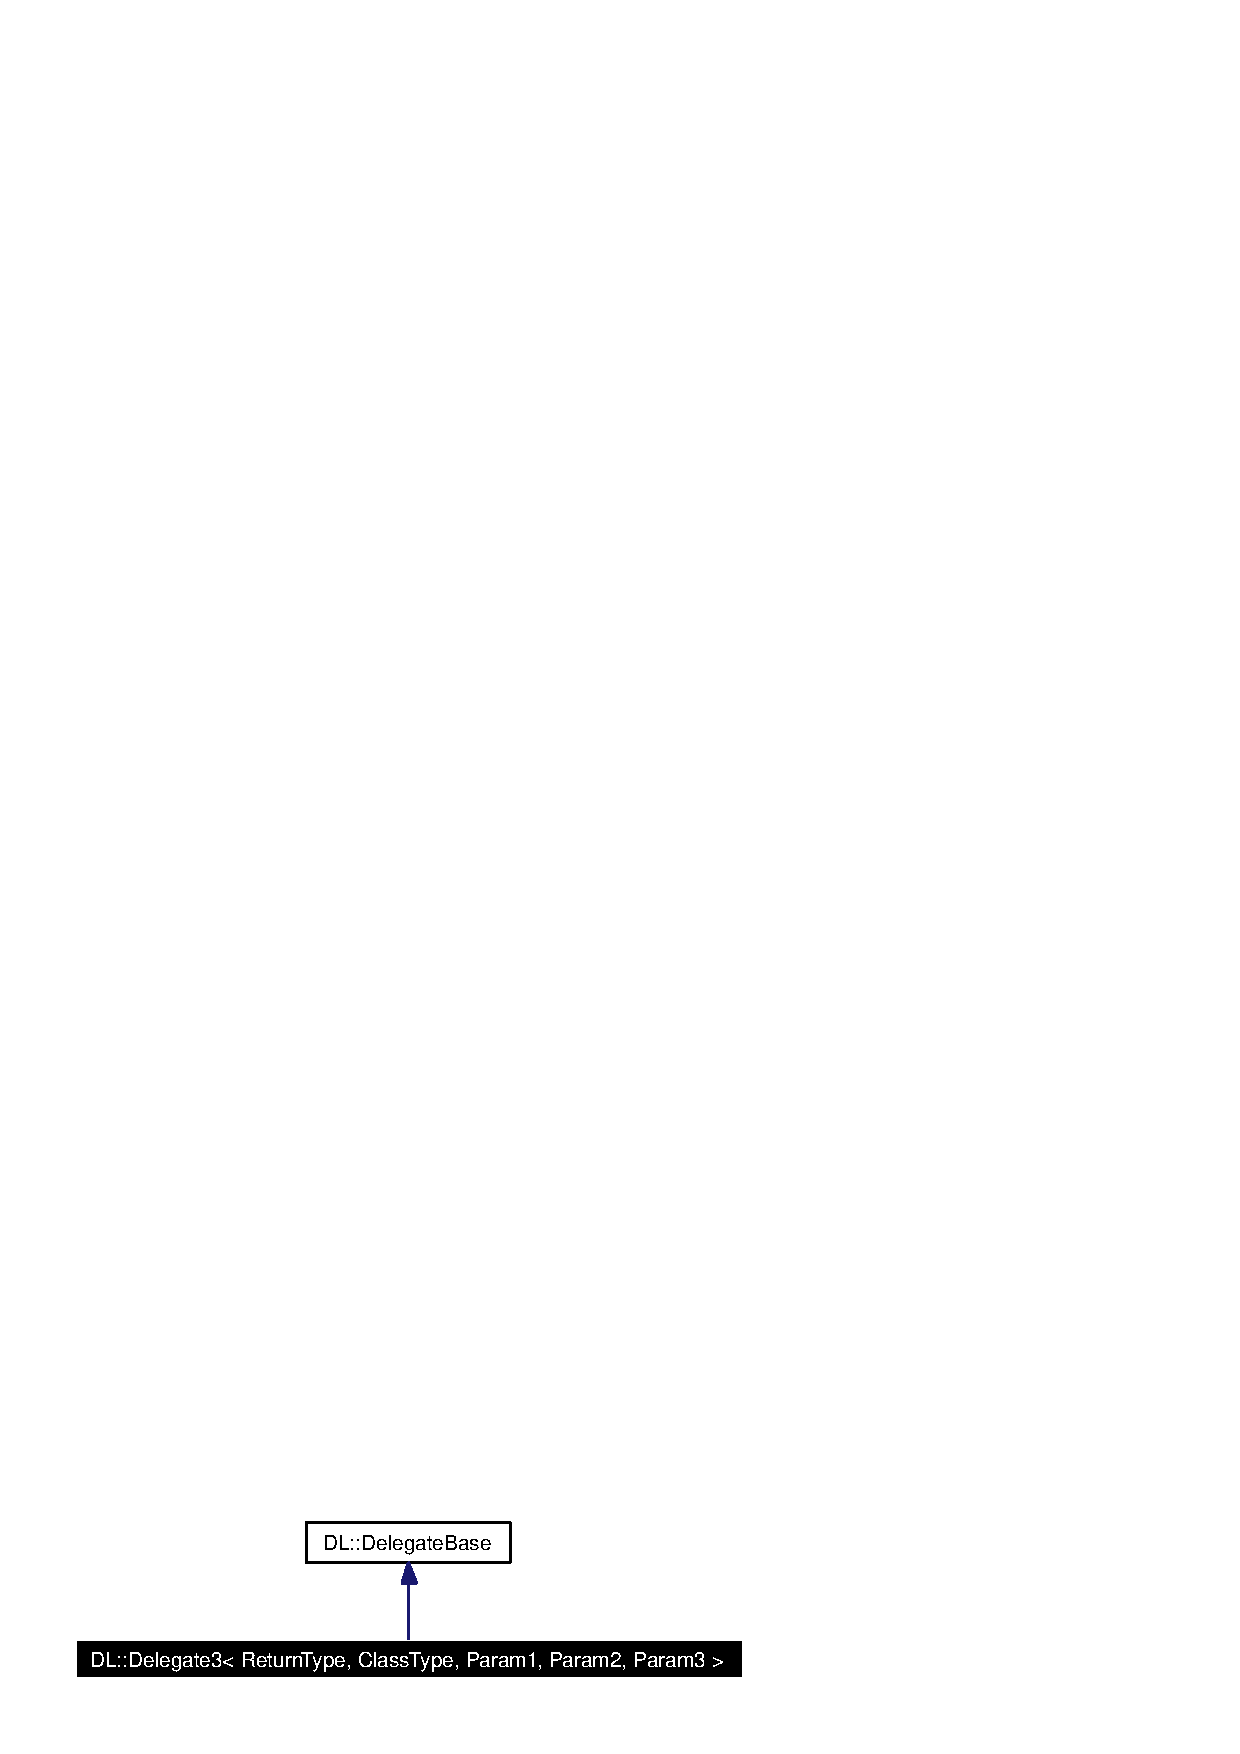
\includegraphics[width=178pt]{classDL_1_1Delegate3__inherit__graph}
\end{center}
\end{figure}
Collaboration diagram for DL::Delegate3$<$ Return\-Type, Class\-Type, Param1, Param2, Param3 $>$:\begin{figure}[H]
\begin{center}
\leavevmode
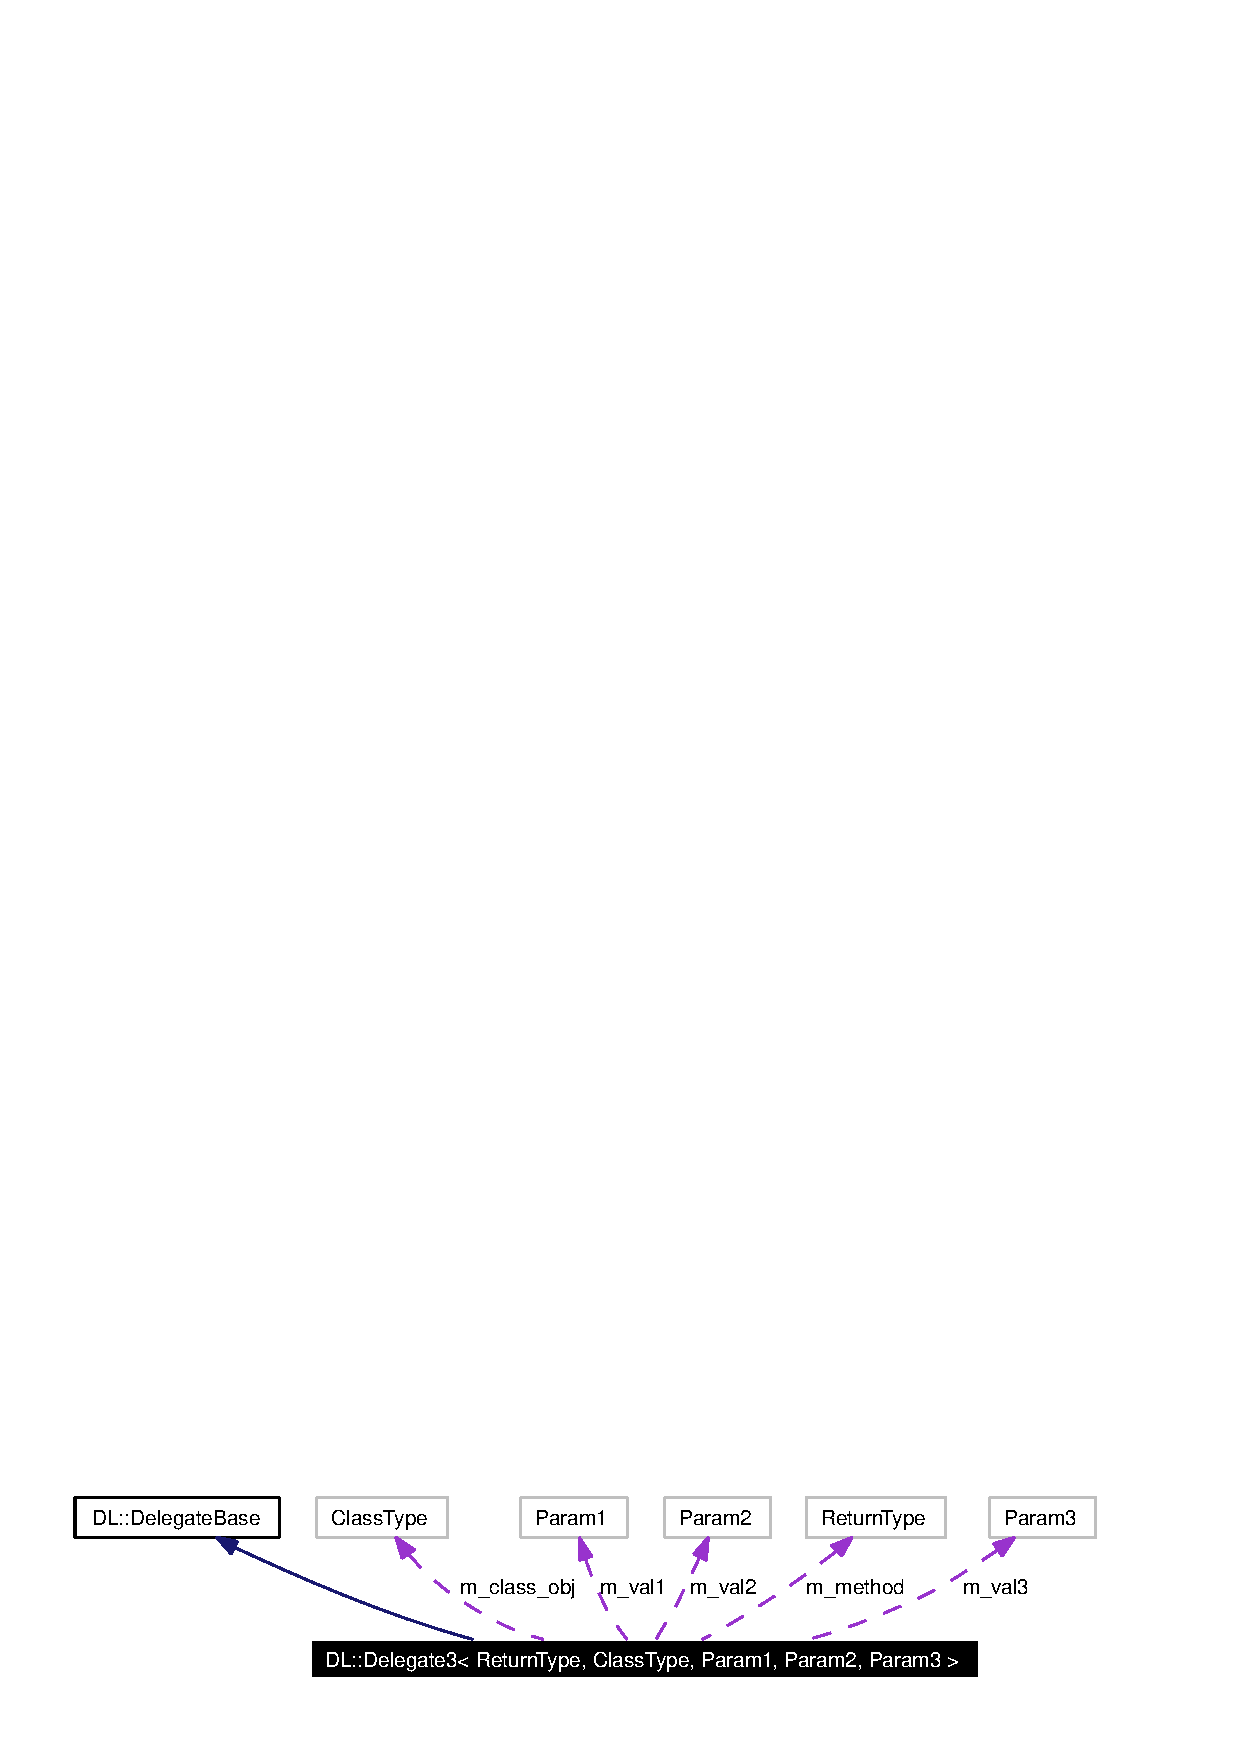
\includegraphics[width=267pt]{classDL_1_1Delegate3__coll__graph}
\end{center}
\end{figure}
\subsection*{Public Member Functions}
\begin{CompactItemize}
\item 
\hyperlink{classDL_1_1Delegate3_a0}{Delegate3} (Class\-Type $\ast$class\_\-obj, Return\-Type(Class\-Type::$\ast$method)(Param1, Param2, Param3), Param1 val1=Param1(), Param2 val2=Param2(), Param3 val3=Param3())
\item 
virtual \hyperlink{classDL_1_1Delegate3_a1}{$\sim$Delegate3} ()
\item 
void \hyperlink{classDL_1_1Delegate3_a2}{Invoke} ()
\item 
void \hyperlink{classDL_1_1Delegate3_a3}{Invoke} (Param1 val1, Param2 val2, Param3 val3)
\end{CompactItemize}
\subsection*{Private Member Functions}
\begin{CompactItemize}
\item 
\hyperlink{classDL_1_1Delegate3_d0}{Delegate3} ()
\end{CompactItemize}
\subsection*{Private Attributes}
\begin{CompactItemize}
\item 
Class\-Type $\ast$ \hyperlink{classDL_1_1Delegate3_r0}{m\_\-class\_\-obj}
\item 
Return\-Type(Class\-Type::$\ast$ \hyperlink{classDL_1_1Delegate3_r1}{m\_\-method} )(Param1, Param2, Param3)
\item 
Param1 \hyperlink{classDL_1_1Delegate3_r2}{m\_\-val1}
\item 
Param2 \hyperlink{classDL_1_1Delegate3_r3}{m\_\-val2}
\item 
Param3 \hyperlink{classDL_1_1Delegate3_r4}{m\_\-val3}
\end{CompactItemize}


\subsection{Detailed Description}
\subsubsection*{template$<$class Return\-Type, class Class\-Type, class Param1, class Param2, class Param3$>$ class DL::Delegate3$<$ Return\-Type, Class\-Type, Param1, Param2, Param3 $>$}

Delegate for 3 Param



Definition at line 36 of file Delegate3.hpp.

\subsection{Constructor \& Destructor Documentation}
\hypertarget{classDL_1_1Delegate3_d0}{
\index{DL::Delegate3@{DL::Delegate3}!Delegate3@{Delegate3}}
\index{Delegate3@{Delegate3}!DL::Delegate3@{DL::Delegate3}}
\subsubsection[Delegate3]{\setlength{\rightskip}{0pt plus 5cm}template$<$class Return\-Type, class Class\-Type, class Param1, class Param2, class Param3$>$ \hyperlink{classDL_1_1Delegate3}{DL::Delegate3}$<$ Return\-Type, Class\-Type, Param1, Param2, Param3 $>$::\hyperlink{classDL_1_1Delegate3}{Delegate3} ()\hspace{0.3cm}{\tt  \mbox{[}inline, private\mbox{]}}}}
\label{classDL_1_1Delegate3_d0}




Definition at line 43 of file Delegate3.hpp.\hypertarget{classDL_1_1Delegate3_a0}{
\index{DL::Delegate3@{DL::Delegate3}!Delegate3@{Delegate3}}
\index{Delegate3@{Delegate3}!DL::Delegate3@{DL::Delegate3}}
\subsubsection[Delegate3]{\setlength{\rightskip}{0pt plus 5cm}template$<$class Return\-Type, class Class\-Type, class Param1, class Param2, class Param3$>$ \hyperlink{classDL_1_1Delegate3}{DL::Delegate3}$<$ Return\-Type, Class\-Type, Param1, Param2, Param3 $>$::\hyperlink{classDL_1_1Delegate3}{Delegate3} (Class\-Type $\ast$ {\em class\_\-obj}, Return\-Type(Class\-Type::$\ast$)(Param1, Param2, Param3) {\em method}, Param1 {\em val1} = {\tt Param1()}, Param2 {\em val2} = {\tt Param2()}, Param3 {\em val3} = {\tt Param3()})\hspace{0.3cm}{\tt  \mbox{[}inline\mbox{]}}}}
\label{classDL_1_1Delegate3_a0}




Definition at line 45 of file Delegate3.hpp.

References DL::Delegate3$<$ Return\-Type, Class\-Type, Param1, Param2, Param3 $>$::m\_\-class\_\-obj, DL::Delegate3$<$ Return\-Type, Class\-Type, Param1, Param2, Param3 $>$::m\_\-method, DL::Delegate3$<$ Return\-Type, Class\-Type, Param1, Param2, Param3 $>$::m\_\-val1, DL::Delegate3$<$ Return\-Type, Class\-Type, Param1, Param2, Param3 $>$::m\_\-val2, and DL::Delegate3$<$ Return\-Type, Class\-Type, Param1, Param2, Param3 $>$::m\_\-val3.\hypertarget{classDL_1_1Delegate3_a1}{
\index{DL::Delegate3@{DL::Delegate3}!~Delegate3@{$\sim$Delegate3}}
\index{~Delegate3@{$\sim$Delegate3}!DL::Delegate3@{DL::Delegate3}}
\subsubsection[$\sim$Delegate3]{\setlength{\rightskip}{0pt plus 5cm}template$<$class Return\-Type, class Class\-Type, class Param1, class Param2, class Param3$>$ virtual \hyperlink{classDL_1_1Delegate3}{DL::Delegate3}$<$ Return\-Type, Class\-Type, Param1, Param2, Param3 $>$::$\sim$\hyperlink{classDL_1_1Delegate3}{Delegate3} ()\hspace{0.3cm}{\tt  \mbox{[}inline, virtual\mbox{]}}}}
\label{classDL_1_1Delegate3_a1}




Definition at line 53 of file Delegate3.hpp.

\subsection{Member Function Documentation}
\hypertarget{classDL_1_1Delegate3_a3}{
\index{DL::Delegate3@{DL::Delegate3}!Invoke@{Invoke}}
\index{Invoke@{Invoke}!DL::Delegate3@{DL::Delegate3}}
\subsubsection[Invoke]{\setlength{\rightskip}{0pt plus 5cm}template$<$class Return\-Type, class Class\-Type, class Param1, class Param2, class Param3$>$ void \hyperlink{classDL_1_1Delegate3}{DL::Delegate3}$<$ Return\-Type, Class\-Type, Param1, Param2, Param3 $>$::Invoke (Param1 {\em val1}, Param2 {\em val2}, Param3 {\em val3})\hspace{0.3cm}{\tt  \mbox{[}inline\mbox{]}}}}
\label{classDL_1_1Delegate3_a3}




Definition at line 58 of file Delegate3.hpp.

References DL::Delegate3$<$ Return\-Type, Class\-Type, Param1, Param2, Param3 $>$::m\_\-class\_\-obj, and DL::Delegate3$<$ Return\-Type, Class\-Type, Param1, Param2, Param3 $>$::m\_\-method.\hypertarget{classDL_1_1Delegate3_a2}{
\index{DL::Delegate3@{DL::Delegate3}!Invoke@{Invoke}}
\index{Invoke@{Invoke}!DL::Delegate3@{DL::Delegate3}}
\subsubsection[Invoke]{\setlength{\rightskip}{0pt plus 5cm}template$<$class Return\-Type, class Class\-Type, class Param1, class Param2, class Param3$>$ void \hyperlink{classDL_1_1Delegate3}{DL::Delegate3}$<$ Return\-Type, Class\-Type, Param1, Param2, Param3 $>$::Invoke ()\hspace{0.3cm}{\tt  \mbox{[}inline, virtual\mbox{]}}}}
\label{classDL_1_1Delegate3_a2}




Implements \hyperlink{classDL_1_1DelegateBase_a2}{DL::Delegate\-Base}.

Definition at line 54 of file Delegate3.hpp.

References DL::Delegate3$<$ Return\-Type, Class\-Type, Param1, Param2, Param3 $>$::m\_\-class\_\-obj, DL::Delegate3$<$ Return\-Type, Class\-Type, Param1, Param2, Param3 $>$::m\_\-method, DL::Delegate3$<$ Return\-Type, Class\-Type, Param1, Param2, Param3 $>$::m\_\-val1, DL::Delegate3$<$ Return\-Type, Class\-Type, Param1, Param2, Param3 $>$::m\_\-val2, and DL::Delegate3$<$ Return\-Type, Class\-Type, Param1, Param2, Param3 $>$::m\_\-val3.

\subsection{Member Data Documentation}
\hypertarget{classDL_1_1Delegate3_r0}{
\index{DL::Delegate3@{DL::Delegate3}!m_class_obj@{m\_\-class\_\-obj}}
\index{m_class_obj@{m\_\-class\_\-obj}!DL::Delegate3@{DL::Delegate3}}
\subsubsection[m\_\-class\_\-obj]{\setlength{\rightskip}{0pt plus 5cm}template$<$class Return\-Type, class Class\-Type, class Param1, class Param2, class Param3$>$ Class\-Type$\ast$ \hyperlink{classDL_1_1Delegate3}{DL::Delegate3}$<$ Return\-Type, Class\-Type, Param1, Param2, Param3 $>$::\hyperlink{classDL_1_1Delegate3_r0}{m\_\-class\_\-obj}\hspace{0.3cm}{\tt  \mbox{[}private\mbox{]}}}}
\label{classDL_1_1Delegate3_r0}




Definition at line 38 of file Delegate3.hpp.

Referenced by DL::Delegate3$<$ Return\-Type, Class\-Type, Param1, Param2, Param3 $>$::Delegate3(), and DL::Delegate3$<$ Return\-Type, Class\-Type, Param1, Param2, Param3 $>$::Invoke().\hypertarget{classDL_1_1Delegate3_r1}{
\index{DL::Delegate3@{DL::Delegate3}!m_method@{m\_\-method}}
\index{m_method@{m\_\-method}!DL::Delegate3@{DL::Delegate3}}
\subsubsection[m\_\-method]{\setlength{\rightskip}{0pt plus 5cm}template$<$class Return\-Type, class Class\-Type, class Param1, class Param2, class Param3$>$ Return\-Type(Class\-Type::$\ast$ \hyperlink{classDL_1_1Delegate3}{DL::Delegate3}$<$ Return\-Type, Class\-Type, Param1, Param2, Param3 $>$::\hyperlink{classDL_1_1Delegate3_r1}{m\_\-method})(Param1, Param2, Param3)\hspace{0.3cm}{\tt  \mbox{[}private\mbox{]}}}}
\label{classDL_1_1Delegate3_r1}




Referenced by DL::Delegate3$<$ Return\-Type, Class\-Type, Param1, Param2, Param3 $>$::Delegate3(), and DL::Delegate3$<$ Return\-Type, Class\-Type, Param1, Param2, Param3 $>$::Invoke().\hypertarget{classDL_1_1Delegate3_r2}{
\index{DL::Delegate3@{DL::Delegate3}!m_val1@{m\_\-val1}}
\index{m_val1@{m\_\-val1}!DL::Delegate3@{DL::Delegate3}}
\subsubsection[m\_\-val1]{\setlength{\rightskip}{0pt plus 5cm}template$<$class Return\-Type, class Class\-Type, class Param1, class Param2, class Param3$>$ Param1 \hyperlink{classDL_1_1Delegate3}{DL::Delegate3}$<$ Return\-Type, Class\-Type, Param1, Param2, Param3 $>$::\hyperlink{classDL_1_1Delegate3_r2}{m\_\-val1}\hspace{0.3cm}{\tt  \mbox{[}private\mbox{]}}}}
\label{classDL_1_1Delegate3_r2}




Definition at line 40 of file Delegate3.hpp.

Referenced by DL::Delegate3$<$ Return\-Type, Class\-Type, Param1, Param2, Param3 $>$::Delegate3(), and DL::Delegate3$<$ Return\-Type, Class\-Type, Param1, Param2, Param3 $>$::Invoke().\hypertarget{classDL_1_1Delegate3_r3}{
\index{DL::Delegate3@{DL::Delegate3}!m_val2@{m\_\-val2}}
\index{m_val2@{m\_\-val2}!DL::Delegate3@{DL::Delegate3}}
\subsubsection[m\_\-val2]{\setlength{\rightskip}{0pt plus 5cm}template$<$class Return\-Type, class Class\-Type, class Param1, class Param2, class Param3$>$ Param2 \hyperlink{classDL_1_1Delegate3}{DL::Delegate3}$<$ Return\-Type, Class\-Type, Param1, Param2, Param3 $>$::\hyperlink{classDL_1_1Delegate3_r3}{m\_\-val2}\hspace{0.3cm}{\tt  \mbox{[}private\mbox{]}}}}
\label{classDL_1_1Delegate3_r3}




Definition at line 41 of file Delegate3.hpp.

Referenced by DL::Delegate3$<$ Return\-Type, Class\-Type, Param1, Param2, Param3 $>$::Delegate3(), and DL::Delegate3$<$ Return\-Type, Class\-Type, Param1, Param2, Param3 $>$::Invoke().\hypertarget{classDL_1_1Delegate3_r4}{
\index{DL::Delegate3@{DL::Delegate3}!m_val3@{m\_\-val3}}
\index{m_val3@{m\_\-val3}!DL::Delegate3@{DL::Delegate3}}
\subsubsection[m\_\-val3]{\setlength{\rightskip}{0pt plus 5cm}template$<$class Return\-Type, class Class\-Type, class Param1, class Param2, class Param3$>$ Param3 \hyperlink{classDL_1_1Delegate3}{DL::Delegate3}$<$ Return\-Type, Class\-Type, Param1, Param2, Param3 $>$::\hyperlink{classDL_1_1Delegate3_r4}{m\_\-val3}\hspace{0.3cm}{\tt  \mbox{[}private\mbox{]}}}}
\label{classDL_1_1Delegate3_r4}




Definition at line 42 of file Delegate3.hpp.

Referenced by DL::Delegate3$<$ Return\-Type, Class\-Type, Param1, Param2, Param3 $>$::Delegate3(), and DL::Delegate3$<$ Return\-Type, Class\-Type, Param1, Param2, Param3 $>$::Invoke().

The documentation for this class was generated from the following file:\begin{CompactItemize}
\item 
/data/callbackext/Delegate\-N/\hyperlink{Delegate3_8hpp}{Delegate3.hpp}\end{CompactItemize}

\hypertarget{classDL_1_1Delegate4}{
\section{DL::Delegate4$<$ Return\-Type, Class\-Type, Param1, Param2, Param3, Param4 $>$ Class Template Reference}
\label{classDL_1_1Delegate4}\index{DL::Delegate4@{DL::Delegate4}}
}
{\tt \#include $<$Delegate4.hpp$>$}

Inherits \hyperlink{classDL_1_1DelegateBase}{DL::Delegate\-Base}.

Inheritance diagram for DL::Delegate4$<$ Return\-Type, Class\-Type, Param1, Param2, Param3, Param4 $>$:\begin{figure}[H]
\begin{center}
\leavevmode
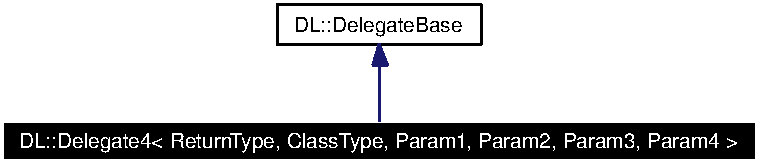
\includegraphics[width=199pt]{classDL_1_1Delegate4__inherit__graph}
\end{center}
\end{figure}
Collaboration diagram for DL::Delegate4$<$ Return\-Type, Class\-Type, Param1, Param2, Param3, Param4 $>$:\begin{figure}[H]
\begin{center}
\leavevmode
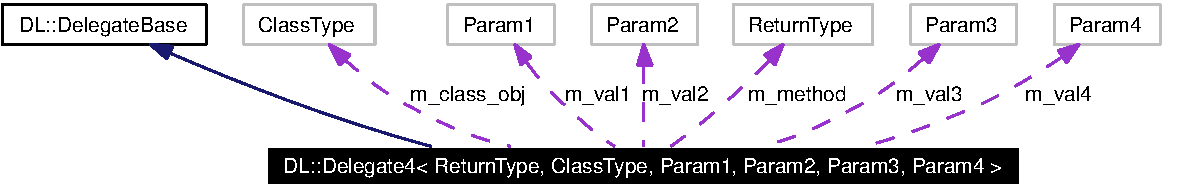
\includegraphics[width=300pt]{classDL_1_1Delegate4__coll__graph}
\end{center}
\end{figure}
\subsection*{Public Member Functions}
\begin{CompactItemize}
\item 
\hyperlink{classDL_1_1Delegate4_a0}{Delegate4} (Class\-Type $\ast$class\_\-obj, Return\-Type(Class\-Type::$\ast$method)(Param1, Param2, Param3, Param4), Param1 val1=Param1(), Param2 val2=Param2(), Param3 val3=Param3(), Param4 val4=Param4())
\item 
virtual \hyperlink{classDL_1_1Delegate4_a1}{$\sim$Delegate4} ()
\item 
void \hyperlink{classDL_1_1Delegate4_a2}{Invoke} ()
\item 
void \hyperlink{classDL_1_1Delegate4_a3}{Invoke} (Param1 val1, Param2 val2, Param3 val3, Param4 val4)
\end{CompactItemize}
\subsection*{Private Member Functions}
\begin{CompactItemize}
\item 
\hyperlink{classDL_1_1Delegate4_d0}{Delegate4} ()
\end{CompactItemize}
\subsection*{Private Attributes}
\begin{CompactItemize}
\item 
Class\-Type $\ast$ \hyperlink{classDL_1_1Delegate4_r0}{m\_\-class\_\-obj}
\item 
Return\-Type(Class\-Type::$\ast$ \hyperlink{classDL_1_1Delegate4_r1}{m\_\-method} )(Param1, Param2, Param3, Param4)
\item 
Param1 \hyperlink{classDL_1_1Delegate4_r2}{m\_\-val1}
\item 
Param2 \hyperlink{classDL_1_1Delegate4_r3}{m\_\-val2}
\item 
Param3 \hyperlink{classDL_1_1Delegate4_r4}{m\_\-val3}
\item 
Param4 \hyperlink{classDL_1_1Delegate4_r5}{m\_\-val4}
\end{CompactItemize}


\subsection{Detailed Description}
\subsubsection*{template$<$class Return\-Type, class Class\-Type, class Param1, class Param2, class Param3, class Param4$>$ class DL::Delegate4$<$ Return\-Type, Class\-Type, Param1, Param2, Param3, Param4 $>$}

Delegate for 4 Param



Definition at line 35 of file Delegate4.hpp.

\subsection{Constructor \& Destructor Documentation}
\hypertarget{classDL_1_1Delegate4_d0}{
\index{DL::Delegate4@{DL::Delegate4}!Delegate4@{Delegate4}}
\index{Delegate4@{Delegate4}!DL::Delegate4@{DL::Delegate4}}
\subsubsection[Delegate4]{\setlength{\rightskip}{0pt plus 5cm}template$<$class Return\-Type, class Class\-Type, class Param1, class Param2, class Param3, class Param4$>$ \hyperlink{classDL_1_1Delegate4}{DL::Delegate4}$<$ Return\-Type, Class\-Type, Param1, Param2, Param3, Param4 $>$::\hyperlink{classDL_1_1Delegate4}{Delegate4} ()\hspace{0.3cm}{\tt  \mbox{[}inline, private\mbox{]}}}}
\label{classDL_1_1Delegate4_d0}




Definition at line 43 of file Delegate4.hpp.\hypertarget{classDL_1_1Delegate4_a0}{
\index{DL::Delegate4@{DL::Delegate4}!Delegate4@{Delegate4}}
\index{Delegate4@{Delegate4}!DL::Delegate4@{DL::Delegate4}}
\subsubsection[Delegate4]{\setlength{\rightskip}{0pt plus 5cm}template$<$class Return\-Type, class Class\-Type, class Param1, class Param2, class Param3, class Param4$>$ \hyperlink{classDL_1_1Delegate4}{DL::Delegate4}$<$ Return\-Type, Class\-Type, Param1, Param2, Param3, Param4 $>$::\hyperlink{classDL_1_1Delegate4}{Delegate4} (Class\-Type $\ast$ {\em class\_\-obj}, Return\-Type(Class\-Type::$\ast$)(Param1, Param2, Param3, Param4) {\em method}, Param1 {\em val1} = {\tt Param1()}, Param2 {\em val2} = {\tt Param2()}, Param3 {\em val3} = {\tt Param3()}, Param4 {\em val4} = {\tt Param4()})\hspace{0.3cm}{\tt  \mbox{[}inline\mbox{]}}}}
\label{classDL_1_1Delegate4_a0}




Definition at line 45 of file Delegate4.hpp.

References DL::Delegate4$<$ Return\-Type, Class\-Type, Param1, Param2, Param3, Param4 $>$::m\_\-class\_\-obj, DL::Delegate4$<$ Return\-Type, Class\-Type, Param1, Param2, Param3, Param4 $>$::m\_\-method, DL::Delegate4$<$ Return\-Type, Class\-Type, Param1, Param2, Param3, Param4 $>$::m\_\-val1, DL::Delegate4$<$ Return\-Type, Class\-Type, Param1, Param2, Param3, Param4 $>$::m\_\-val2, DL::Delegate4$<$ Return\-Type, Class\-Type, Param1, Param2, Param3, Param4 $>$::m\_\-val3, and DL::Delegate4$<$ Return\-Type, Class\-Type, Param1, Param2, Param3, Param4 $>$::m\_\-val4.\hypertarget{classDL_1_1Delegate4_a1}{
\index{DL::Delegate4@{DL::Delegate4}!~Delegate4@{$\sim$Delegate4}}
\index{~Delegate4@{$\sim$Delegate4}!DL::Delegate4@{DL::Delegate4}}
\subsubsection[$\sim$Delegate4]{\setlength{\rightskip}{0pt plus 5cm}template$<$class Return\-Type, class Class\-Type, class Param1, class Param2, class Param3, class Param4$>$ virtual \hyperlink{classDL_1_1Delegate4}{DL::Delegate4}$<$ Return\-Type, Class\-Type, Param1, Param2, Param3, Param4 $>$::$\sim$\hyperlink{classDL_1_1Delegate4}{Delegate4} ()\hspace{0.3cm}{\tt  \mbox{[}inline, virtual\mbox{]}}}}
\label{classDL_1_1Delegate4_a1}




Definition at line 55 of file Delegate4.hpp.

\subsection{Member Function Documentation}
\hypertarget{classDL_1_1Delegate4_a3}{
\index{DL::Delegate4@{DL::Delegate4}!Invoke@{Invoke}}
\index{Invoke@{Invoke}!DL::Delegate4@{DL::Delegate4}}
\subsubsection[Invoke]{\setlength{\rightskip}{0pt plus 5cm}template$<$class Return\-Type, class Class\-Type, class Param1, class Param2, class Param3, class Param4$>$ void \hyperlink{classDL_1_1Delegate4}{DL::Delegate4}$<$ Return\-Type, Class\-Type, Param1, Param2, Param3, Param4 $>$::Invoke (Param1 {\em val1}, Param2 {\em val2}, Param3 {\em val3}, Param4 {\em val4})\hspace{0.3cm}{\tt  \mbox{[}inline\mbox{]}}}}
\label{classDL_1_1Delegate4_a3}




Definition at line 60 of file Delegate4.hpp.

References DL::Delegate4$<$ Return\-Type, Class\-Type, Param1, Param2, Param3, Param4 $>$::m\_\-class\_\-obj, and DL::Delegate4$<$ Return\-Type, Class\-Type, Param1, Param2, Param3, Param4 $>$::m\_\-method.\hypertarget{classDL_1_1Delegate4_a2}{
\index{DL::Delegate4@{DL::Delegate4}!Invoke@{Invoke}}
\index{Invoke@{Invoke}!DL::Delegate4@{DL::Delegate4}}
\subsubsection[Invoke]{\setlength{\rightskip}{0pt plus 5cm}template$<$class Return\-Type, class Class\-Type, class Param1, class Param2, class Param3, class Param4$>$ void \hyperlink{classDL_1_1Delegate4}{DL::Delegate4}$<$ Return\-Type, Class\-Type, Param1, Param2, Param3, Param4 $>$::Invoke ()\hspace{0.3cm}{\tt  \mbox{[}inline, virtual\mbox{]}}}}
\label{classDL_1_1Delegate4_a2}




Implements \hyperlink{classDL_1_1DelegateBase_a2}{DL::Delegate\-Base}.

Definition at line 56 of file Delegate4.hpp.

References DL::Delegate4$<$ Return\-Type, Class\-Type, Param1, Param2, Param3, Param4 $>$::m\_\-class\_\-obj, DL::Delegate4$<$ Return\-Type, Class\-Type, Param1, Param2, Param3, Param4 $>$::m\_\-method, DL::Delegate4$<$ Return\-Type, Class\-Type, Param1, Param2, Param3, Param4 $>$::m\_\-val1, DL::Delegate4$<$ Return\-Type, Class\-Type, Param1, Param2, Param3, Param4 $>$::m\_\-val2, DL::Delegate4$<$ Return\-Type, Class\-Type, Param1, Param2, Param3, Param4 $>$::m\_\-val3, and DL::Delegate4$<$ Return\-Type, Class\-Type, Param1, Param2, Param3, Param4 $>$::m\_\-val4.

\subsection{Member Data Documentation}
\hypertarget{classDL_1_1Delegate4_r0}{
\index{DL::Delegate4@{DL::Delegate4}!m_class_obj@{m\_\-class\_\-obj}}
\index{m_class_obj@{m\_\-class\_\-obj}!DL::Delegate4@{DL::Delegate4}}
\subsubsection[m\_\-class\_\-obj]{\setlength{\rightskip}{0pt plus 5cm}template$<$class Return\-Type, class Class\-Type, class Param1, class Param2, class Param3, class Param4$>$ Class\-Type$\ast$ \hyperlink{classDL_1_1Delegate4}{DL::Delegate4}$<$ Return\-Type, Class\-Type, Param1, Param2, Param3, Param4 $>$::\hyperlink{classDL_1_1Delegate4_r0}{m\_\-class\_\-obj}\hspace{0.3cm}{\tt  \mbox{[}private\mbox{]}}}}
\label{classDL_1_1Delegate4_r0}




Definition at line 37 of file Delegate4.hpp.

Referenced by DL::Delegate4$<$ Return\-Type, Class\-Type, Param1, Param2, Param3, Param4 $>$::Delegate4(), and DL::Delegate4$<$ Return\-Type, Class\-Type, Param1, Param2, Param3, Param4 $>$::Invoke().\hypertarget{classDL_1_1Delegate4_r1}{
\index{DL::Delegate4@{DL::Delegate4}!m_method@{m\_\-method}}
\index{m_method@{m\_\-method}!DL::Delegate4@{DL::Delegate4}}
\subsubsection[m\_\-method]{\setlength{\rightskip}{0pt plus 5cm}template$<$class Return\-Type, class Class\-Type, class Param1, class Param2, class Param3, class Param4$>$ Return\-Type(Class\-Type::$\ast$ \hyperlink{classDL_1_1Delegate4}{DL::Delegate4}$<$ Return\-Type, Class\-Type, Param1, Param2, Param3, Param4 $>$::\hyperlink{classDL_1_1Delegate4_r1}{m\_\-method})(Param1, Param2, Param3, Param4)\hspace{0.3cm}{\tt  \mbox{[}private\mbox{]}}}}
\label{classDL_1_1Delegate4_r1}




Referenced by DL::Delegate4$<$ Return\-Type, Class\-Type, Param1, Param2, Param3, Param4 $>$::Delegate4(), and DL::Delegate4$<$ Return\-Type, Class\-Type, Param1, Param2, Param3, Param4 $>$::Invoke().\hypertarget{classDL_1_1Delegate4_r2}{
\index{DL::Delegate4@{DL::Delegate4}!m_val1@{m\_\-val1}}
\index{m_val1@{m\_\-val1}!DL::Delegate4@{DL::Delegate4}}
\subsubsection[m\_\-val1]{\setlength{\rightskip}{0pt plus 5cm}template$<$class Return\-Type, class Class\-Type, class Param1, class Param2, class Param3, class Param4$>$ Param1 \hyperlink{classDL_1_1Delegate4}{DL::Delegate4}$<$ Return\-Type, Class\-Type, Param1, Param2, Param3, Param4 $>$::\hyperlink{classDL_1_1Delegate4_r2}{m\_\-val1}\hspace{0.3cm}{\tt  \mbox{[}private\mbox{]}}}}
\label{classDL_1_1Delegate4_r2}




Definition at line 39 of file Delegate4.hpp.

Referenced by DL::Delegate4$<$ Return\-Type, Class\-Type, Param1, Param2, Param3, Param4 $>$::Delegate4(), and DL::Delegate4$<$ Return\-Type, Class\-Type, Param1, Param2, Param3, Param4 $>$::Invoke().\hypertarget{classDL_1_1Delegate4_r3}{
\index{DL::Delegate4@{DL::Delegate4}!m_val2@{m\_\-val2}}
\index{m_val2@{m\_\-val2}!DL::Delegate4@{DL::Delegate4}}
\subsubsection[m\_\-val2]{\setlength{\rightskip}{0pt plus 5cm}template$<$class Return\-Type, class Class\-Type, class Param1, class Param2, class Param3, class Param4$>$ Param2 \hyperlink{classDL_1_1Delegate4}{DL::Delegate4}$<$ Return\-Type, Class\-Type, Param1, Param2, Param3, Param4 $>$::\hyperlink{classDL_1_1Delegate4_r3}{m\_\-val2}\hspace{0.3cm}{\tt  \mbox{[}private\mbox{]}}}}
\label{classDL_1_1Delegate4_r3}




Definition at line 40 of file Delegate4.hpp.

Referenced by DL::Delegate4$<$ Return\-Type, Class\-Type, Param1, Param2, Param3, Param4 $>$::Delegate4(), and DL::Delegate4$<$ Return\-Type, Class\-Type, Param1, Param2, Param3, Param4 $>$::Invoke().\hypertarget{classDL_1_1Delegate4_r4}{
\index{DL::Delegate4@{DL::Delegate4}!m_val3@{m\_\-val3}}
\index{m_val3@{m\_\-val3}!DL::Delegate4@{DL::Delegate4}}
\subsubsection[m\_\-val3]{\setlength{\rightskip}{0pt plus 5cm}template$<$class Return\-Type, class Class\-Type, class Param1, class Param2, class Param3, class Param4$>$ Param3 \hyperlink{classDL_1_1Delegate4}{DL::Delegate4}$<$ Return\-Type, Class\-Type, Param1, Param2, Param3, Param4 $>$::\hyperlink{classDL_1_1Delegate4_r4}{m\_\-val3}\hspace{0.3cm}{\tt  \mbox{[}private\mbox{]}}}}
\label{classDL_1_1Delegate4_r4}




Definition at line 41 of file Delegate4.hpp.

Referenced by DL::Delegate4$<$ Return\-Type, Class\-Type, Param1, Param2, Param3, Param4 $>$::Delegate4(), and DL::Delegate4$<$ Return\-Type, Class\-Type, Param1, Param2, Param3, Param4 $>$::Invoke().\hypertarget{classDL_1_1Delegate4_r5}{
\index{DL::Delegate4@{DL::Delegate4}!m_val4@{m\_\-val4}}
\index{m_val4@{m\_\-val4}!DL::Delegate4@{DL::Delegate4}}
\subsubsection[m\_\-val4]{\setlength{\rightskip}{0pt plus 5cm}template$<$class Return\-Type, class Class\-Type, class Param1, class Param2, class Param3, class Param4$>$ Param4 \hyperlink{classDL_1_1Delegate4}{DL::Delegate4}$<$ Return\-Type, Class\-Type, Param1, Param2, Param3, Param4 $>$::\hyperlink{classDL_1_1Delegate4_r5}{m\_\-val4}\hspace{0.3cm}{\tt  \mbox{[}private\mbox{]}}}}
\label{classDL_1_1Delegate4_r5}




Definition at line 42 of file Delegate4.hpp.

Referenced by DL::Delegate4$<$ Return\-Type, Class\-Type, Param1, Param2, Param3, Param4 $>$::Delegate4(), and DL::Delegate4$<$ Return\-Type, Class\-Type, Param1, Param2, Param3, Param4 $>$::Invoke().

The documentation for this class was generated from the following file:\begin{CompactItemize}
\item 
/data/callbackext/Delegate\-N/\hyperlink{Delegate4_8hpp}{Delegate4.hpp}\end{CompactItemize}

\hypertarget{classDL_1_1Delegate5}{
\section{DL::Delegate5$<$ Return\-Type, Class\-Type, Param1, Param2, Param3, Param4, Param5 $>$ Class Template Reference}
\label{classDL_1_1Delegate5}\index{DL::Delegate5@{DL::Delegate5}}
}
{\tt \#include $<$Delegate5.hpp$>$}

Inherits \hyperlink{classDL_1_1DelegateBase}{DL::Delegate\-Base}.

Inheritance diagram for DL::Delegate5$<$ Return\-Type, Class\-Type, Param1, Param2, Param3, Param4, Param5 $>$:\begin{figure}[H]
\begin{center}
\leavevmode
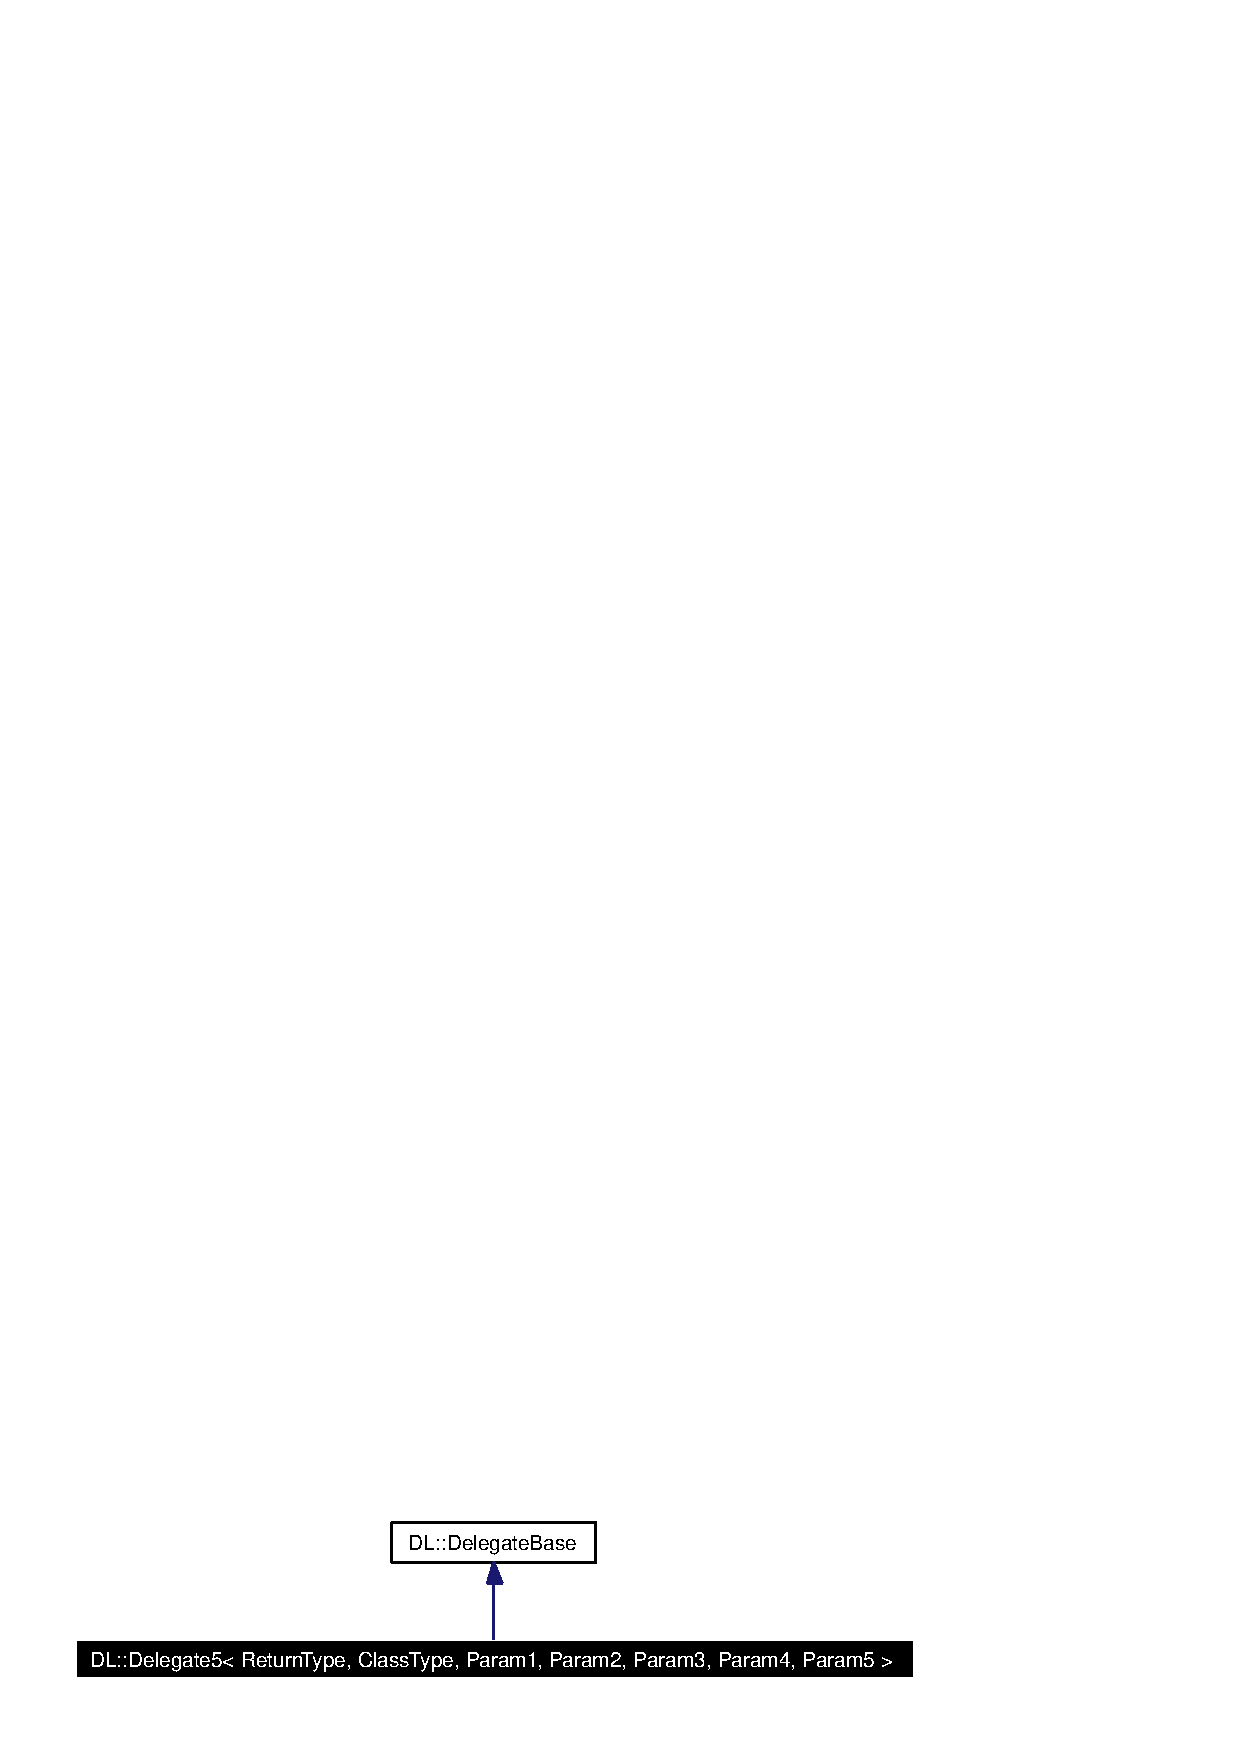
\includegraphics[width=219pt]{classDL_1_1Delegate5__inherit__graph}
\end{center}
\end{figure}
Collaboration diagram for DL::Delegate5$<$ Return\-Type, Class\-Type, Param1, Param2, Param3, Param4, Param5 $>$:\begin{figure}[H]
\begin{center}
\leavevmode
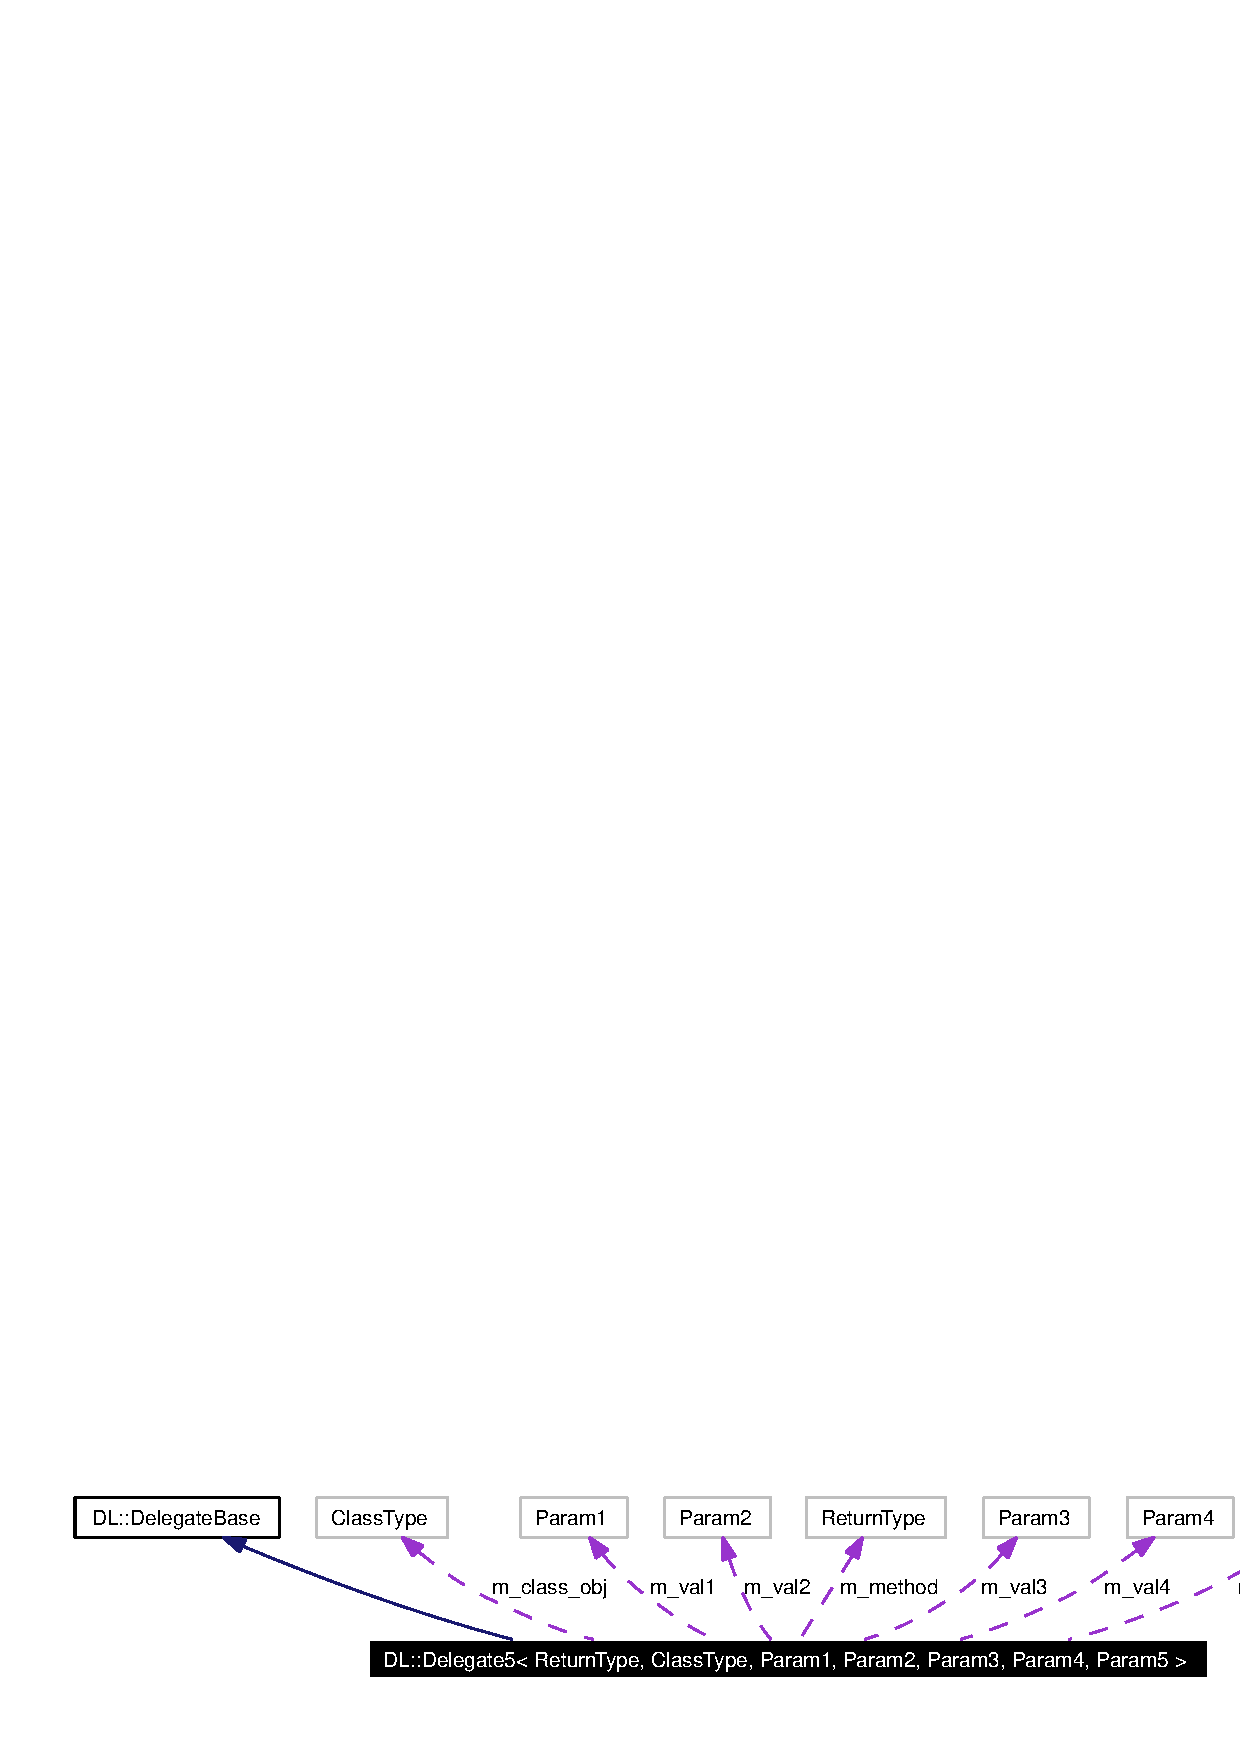
\includegraphics[width=334pt]{classDL_1_1Delegate5__coll__graph}
\end{center}
\end{figure}
\subsection*{Public Member Functions}
\begin{CompactItemize}
\item 
\hyperlink{classDL_1_1Delegate5_a0}{Delegate5} (Class\-Type $\ast$class\_\-obj, Return\-Type(Class\-Type::$\ast$method)(Param1, Param2, Param3, Param4, Param5), Param1 val1=Param1(), Param2 val2=Param2(), Param3 val3=Param3(), Param4 val4=Param4(), Param5 val5=Param5())
\item 
virtual \hyperlink{classDL_1_1Delegate5_a1}{$\sim$Delegate5} ()
\item 
void \hyperlink{classDL_1_1Delegate5_a2}{Invoke} ()
\item 
void \hyperlink{classDL_1_1Delegate5_a3}{Invoke} (Param1 val1, Param2 val2, Param3 val3, Param4 val4, Param5 val5)
\end{CompactItemize}
\subsection*{Private Member Functions}
\begin{CompactItemize}
\item 
\hyperlink{classDL_1_1Delegate5_d0}{Delegate5} ()
\end{CompactItemize}
\subsection*{Private Attributes}
\begin{CompactItemize}
\item 
Class\-Type $\ast$ \hyperlink{classDL_1_1Delegate5_r0}{m\_\-class\_\-obj}
\item 
Return\-Type(Class\-Type::$\ast$ \hyperlink{classDL_1_1Delegate5_r1}{m\_\-method} )(Param1, Param2, Param3, Param4, Param5)
\item 
Param1 \hyperlink{classDL_1_1Delegate5_r2}{m\_\-val1}
\item 
Param2 \hyperlink{classDL_1_1Delegate5_r3}{m\_\-val2}
\item 
Param3 \hyperlink{classDL_1_1Delegate5_r4}{m\_\-val3}
\item 
Param4 \hyperlink{classDL_1_1Delegate5_r5}{m\_\-val4}
\item 
Param5 \hyperlink{classDL_1_1Delegate5_r6}{m\_\-val5}
\end{CompactItemize}


\subsection{Detailed Description}
\subsubsection*{template$<$class Return\-Type, class Class\-Type, class Param1, class Param2, class Param3, class Param4, class Param5$>$ class DL::Delegate5$<$ Return\-Type, Class\-Type, Param1, Param2, Param3, Param4, Param5 $>$}

Delegate for 5 Param



Definition at line 36 of file Delegate5.hpp.

\subsection{Constructor \& Destructor Documentation}
\hypertarget{classDL_1_1Delegate5_d0}{
\index{DL::Delegate5@{DL::Delegate5}!Delegate5@{Delegate5}}
\index{Delegate5@{Delegate5}!DL::Delegate5@{DL::Delegate5}}
\subsubsection[Delegate5]{\setlength{\rightskip}{0pt plus 5cm}template$<$class Return\-Type, class Class\-Type, class Param1, class Param2, class Param3, class Param4, class Param5$>$ \hyperlink{classDL_1_1Delegate5}{DL::Delegate5}$<$ Return\-Type, Class\-Type, Param1, Param2, Param3, Param4, Param5 $>$::\hyperlink{classDL_1_1Delegate5}{Delegate5} ()\hspace{0.3cm}{\tt  \mbox{[}inline, private\mbox{]}}}}
\label{classDL_1_1Delegate5_d0}




Definition at line 45 of file Delegate5.hpp.\hypertarget{classDL_1_1Delegate5_a0}{
\index{DL::Delegate5@{DL::Delegate5}!Delegate5@{Delegate5}}
\index{Delegate5@{Delegate5}!DL::Delegate5@{DL::Delegate5}}
\subsubsection[Delegate5]{\setlength{\rightskip}{0pt plus 5cm}template$<$class Return\-Type, class Class\-Type, class Param1, class Param2, class Param3, class Param4, class Param5$>$ \hyperlink{classDL_1_1Delegate5}{DL::Delegate5}$<$ Return\-Type, Class\-Type, Param1, Param2, Param3, Param4, Param5 $>$::\hyperlink{classDL_1_1Delegate5}{Delegate5} (Class\-Type $\ast$ {\em class\_\-obj}, Return\-Type(Class\-Type::$\ast$)(Param1, Param2, Param3, Param4, Param5) {\em method}, Param1 {\em val1} = {\tt Param1()}, Param2 {\em val2} = {\tt Param2()}, Param3 {\em val3} = {\tt Param3()}, Param4 {\em val4} = {\tt Param4()}, Param5 {\em val5} = {\tt Param5()})\hspace{0.3cm}{\tt  \mbox{[}inline\mbox{]}}}}
\label{classDL_1_1Delegate5_a0}




Definition at line 47 of file Delegate5.hpp.

References DL::Delegate5$<$ Return\-Type, Class\-Type, Param1, Param2, Param3, Param4, Param5 $>$::m\_\-class\_\-obj, DL::Delegate5$<$ Return\-Type, Class\-Type, Param1, Param2, Param3, Param4, Param5 $>$::m\_\-method, DL::Delegate5$<$ Return\-Type, Class\-Type, Param1, Param2, Param3, Param4, Param5 $>$::m\_\-val1, DL::Delegate5$<$ Return\-Type, Class\-Type, Param1, Param2, Param3, Param4, Param5 $>$::m\_\-val2, DL::Delegate5$<$ Return\-Type, Class\-Type, Param1, Param2, Param3, Param4, Param5 $>$::m\_\-val3, DL::Delegate5$<$ Return\-Type, Class\-Type, Param1, Param2, Param3, Param4, Param5 $>$::m\_\-val4, and DL::Delegate5$<$ Return\-Type, Class\-Type, Param1, Param2, Param3, Param4, Param5 $>$::m\_\-val5.\hypertarget{classDL_1_1Delegate5_a1}{
\index{DL::Delegate5@{DL::Delegate5}!~Delegate5@{$\sim$Delegate5}}
\index{~Delegate5@{$\sim$Delegate5}!DL::Delegate5@{DL::Delegate5}}
\subsubsection[$\sim$Delegate5]{\setlength{\rightskip}{0pt plus 5cm}template$<$class Return\-Type, class Class\-Type, class Param1, class Param2, class Param3, class Param4, class Param5$>$ virtual \hyperlink{classDL_1_1Delegate5}{DL::Delegate5}$<$ Return\-Type, Class\-Type, Param1, Param2, Param3, Param4, Param5 $>$::$\sim$\hyperlink{classDL_1_1Delegate5}{Delegate5} ()\hspace{0.3cm}{\tt  \mbox{[}inline, virtual\mbox{]}}}}
\label{classDL_1_1Delegate5_a1}




Definition at line 58 of file Delegate5.hpp.

\subsection{Member Function Documentation}
\hypertarget{classDL_1_1Delegate5_a3}{
\index{DL::Delegate5@{DL::Delegate5}!Invoke@{Invoke}}
\index{Invoke@{Invoke}!DL::Delegate5@{DL::Delegate5}}
\subsubsection[Invoke]{\setlength{\rightskip}{0pt plus 5cm}template$<$class Return\-Type, class Class\-Type, class Param1, class Param2, class Param3, class Param4, class Param5$>$ void \hyperlink{classDL_1_1Delegate5}{DL::Delegate5}$<$ Return\-Type, Class\-Type, Param1, Param2, Param3, Param4, Param5 $>$::Invoke (Param1 {\em val1}, Param2 {\em val2}, Param3 {\em val3}, Param4 {\em val4}, Param5 {\em val5})\hspace{0.3cm}{\tt  \mbox{[}inline\mbox{]}}}}
\label{classDL_1_1Delegate5_a3}




Definition at line 63 of file Delegate5.hpp.

References DL::Delegate5$<$ Return\-Type, Class\-Type, Param1, Param2, Param3, Param4, Param5 $>$::m\_\-class\_\-obj, and DL::Delegate5$<$ Return\-Type, Class\-Type, Param1, Param2, Param3, Param4, Param5 $>$::m\_\-method.\hypertarget{classDL_1_1Delegate5_a2}{
\index{DL::Delegate5@{DL::Delegate5}!Invoke@{Invoke}}
\index{Invoke@{Invoke}!DL::Delegate5@{DL::Delegate5}}
\subsubsection[Invoke]{\setlength{\rightskip}{0pt plus 5cm}template$<$class Return\-Type, class Class\-Type, class Param1, class Param2, class Param3, class Param4, class Param5$>$ void \hyperlink{classDL_1_1Delegate5}{DL::Delegate5}$<$ Return\-Type, Class\-Type, Param1, Param2, Param3, Param4, Param5 $>$::Invoke ()\hspace{0.3cm}{\tt  \mbox{[}inline, virtual\mbox{]}}}}
\label{classDL_1_1Delegate5_a2}




Implements \hyperlink{classDL_1_1DelegateBase_a2}{DL::Delegate\-Base}.

Definition at line 59 of file Delegate5.hpp.

References DL::Delegate5$<$ Return\-Type, Class\-Type, Param1, Param2, Param3, Param4, Param5 $>$::m\_\-class\_\-obj, DL::Delegate5$<$ Return\-Type, Class\-Type, Param1, Param2, Param3, Param4, Param5 $>$::m\_\-method, DL::Delegate5$<$ Return\-Type, Class\-Type, Param1, Param2, Param3, Param4, Param5 $>$::m\_\-val1, DL::Delegate5$<$ Return\-Type, Class\-Type, Param1, Param2, Param3, Param4, Param5 $>$::m\_\-val2, DL::Delegate5$<$ Return\-Type, Class\-Type, Param1, Param2, Param3, Param4, Param5 $>$::m\_\-val3, DL::Delegate5$<$ Return\-Type, Class\-Type, Param1, Param2, Param3, Param4, Param5 $>$::m\_\-val4, and DL::Delegate5$<$ Return\-Type, Class\-Type, Param1, Param2, Param3, Param4, Param5 $>$::m\_\-val5.

\subsection{Member Data Documentation}
\hypertarget{classDL_1_1Delegate5_r0}{
\index{DL::Delegate5@{DL::Delegate5}!m_class_obj@{m\_\-class\_\-obj}}
\index{m_class_obj@{m\_\-class\_\-obj}!DL::Delegate5@{DL::Delegate5}}
\subsubsection[m\_\-class\_\-obj]{\setlength{\rightskip}{0pt plus 5cm}template$<$class Return\-Type, class Class\-Type, class Param1, class Param2, class Param3, class Param4, class Param5$>$ Class\-Type$\ast$ \hyperlink{classDL_1_1Delegate5}{DL::Delegate5}$<$ Return\-Type, Class\-Type, Param1, Param2, Param3, Param4, Param5 $>$::\hyperlink{classDL_1_1Delegate5_r0}{m\_\-class\_\-obj}\hspace{0.3cm}{\tt  \mbox{[}private\mbox{]}}}}
\label{classDL_1_1Delegate5_r0}




Definition at line 38 of file Delegate5.hpp.

Referenced by DL::Delegate5$<$ Return\-Type, Class\-Type, Param1, Param2, Param3, Param4, Param5 $>$::Delegate5(), and DL::Delegate5$<$ Return\-Type, Class\-Type, Param1, Param2, Param3, Param4, Param5 $>$::Invoke().\hypertarget{classDL_1_1Delegate5_r1}{
\index{DL::Delegate5@{DL::Delegate5}!m_method@{m\_\-method}}
\index{m_method@{m\_\-method}!DL::Delegate5@{DL::Delegate5}}
\subsubsection[m\_\-method]{\setlength{\rightskip}{0pt plus 5cm}template$<$class Return\-Type, class Class\-Type, class Param1, class Param2, class Param3, class Param4, class Param5$>$ Return\-Type(Class\-Type::$\ast$ \hyperlink{classDL_1_1Delegate5}{DL::Delegate5}$<$ Return\-Type, Class\-Type, Param1, Param2, Param3, Param4, Param5 $>$::\hyperlink{classDL_1_1Delegate5_r1}{m\_\-method})(Param1, Param2, Param3, Param4, Param5)\hspace{0.3cm}{\tt  \mbox{[}private\mbox{]}}}}
\label{classDL_1_1Delegate5_r1}




Referenced by DL::Delegate5$<$ Return\-Type, Class\-Type, Param1, Param2, Param3, Param4, Param5 $>$::Delegate5(), and DL::Delegate5$<$ Return\-Type, Class\-Type, Param1, Param2, Param3, Param4, Param5 $>$::Invoke().\hypertarget{classDL_1_1Delegate5_r2}{
\index{DL::Delegate5@{DL::Delegate5}!m_val1@{m\_\-val1}}
\index{m_val1@{m\_\-val1}!DL::Delegate5@{DL::Delegate5}}
\subsubsection[m\_\-val1]{\setlength{\rightskip}{0pt plus 5cm}template$<$class Return\-Type, class Class\-Type, class Param1, class Param2, class Param3, class Param4, class Param5$>$ Param1 \hyperlink{classDL_1_1Delegate5}{DL::Delegate5}$<$ Return\-Type, Class\-Type, Param1, Param2, Param3, Param4, Param5 $>$::\hyperlink{classDL_1_1Delegate5_r2}{m\_\-val1}\hspace{0.3cm}{\tt  \mbox{[}private\mbox{]}}}}
\label{classDL_1_1Delegate5_r2}




Definition at line 40 of file Delegate5.hpp.

Referenced by DL::Delegate5$<$ Return\-Type, Class\-Type, Param1, Param2, Param3, Param4, Param5 $>$::Delegate5(), and DL::Delegate5$<$ Return\-Type, Class\-Type, Param1, Param2, Param3, Param4, Param5 $>$::Invoke().\hypertarget{classDL_1_1Delegate5_r3}{
\index{DL::Delegate5@{DL::Delegate5}!m_val2@{m\_\-val2}}
\index{m_val2@{m\_\-val2}!DL::Delegate5@{DL::Delegate5}}
\subsubsection[m\_\-val2]{\setlength{\rightskip}{0pt plus 5cm}template$<$class Return\-Type, class Class\-Type, class Param1, class Param2, class Param3, class Param4, class Param5$>$ Param2 \hyperlink{classDL_1_1Delegate5}{DL::Delegate5}$<$ Return\-Type, Class\-Type, Param1, Param2, Param3, Param4, Param5 $>$::\hyperlink{classDL_1_1Delegate5_r3}{m\_\-val2}\hspace{0.3cm}{\tt  \mbox{[}private\mbox{]}}}}
\label{classDL_1_1Delegate5_r3}




Definition at line 41 of file Delegate5.hpp.

Referenced by DL::Delegate5$<$ Return\-Type, Class\-Type, Param1, Param2, Param3, Param4, Param5 $>$::Delegate5(), and DL::Delegate5$<$ Return\-Type, Class\-Type, Param1, Param2, Param3, Param4, Param5 $>$::Invoke().\hypertarget{classDL_1_1Delegate5_r4}{
\index{DL::Delegate5@{DL::Delegate5}!m_val3@{m\_\-val3}}
\index{m_val3@{m\_\-val3}!DL::Delegate5@{DL::Delegate5}}
\subsubsection[m\_\-val3]{\setlength{\rightskip}{0pt plus 5cm}template$<$class Return\-Type, class Class\-Type, class Param1, class Param2, class Param3, class Param4, class Param5$>$ Param3 \hyperlink{classDL_1_1Delegate5}{DL::Delegate5}$<$ Return\-Type, Class\-Type, Param1, Param2, Param3, Param4, Param5 $>$::\hyperlink{classDL_1_1Delegate5_r4}{m\_\-val3}\hspace{0.3cm}{\tt  \mbox{[}private\mbox{]}}}}
\label{classDL_1_1Delegate5_r4}




Definition at line 42 of file Delegate5.hpp.

Referenced by DL::Delegate5$<$ Return\-Type, Class\-Type, Param1, Param2, Param3, Param4, Param5 $>$::Delegate5(), and DL::Delegate5$<$ Return\-Type, Class\-Type, Param1, Param2, Param3, Param4, Param5 $>$::Invoke().\hypertarget{classDL_1_1Delegate5_r5}{
\index{DL::Delegate5@{DL::Delegate5}!m_val4@{m\_\-val4}}
\index{m_val4@{m\_\-val4}!DL::Delegate5@{DL::Delegate5}}
\subsubsection[m\_\-val4]{\setlength{\rightskip}{0pt plus 5cm}template$<$class Return\-Type, class Class\-Type, class Param1, class Param2, class Param3, class Param4, class Param5$>$ Param4 \hyperlink{classDL_1_1Delegate5}{DL::Delegate5}$<$ Return\-Type, Class\-Type, Param1, Param2, Param3, Param4, Param5 $>$::\hyperlink{classDL_1_1Delegate5_r5}{m\_\-val4}\hspace{0.3cm}{\tt  \mbox{[}private\mbox{]}}}}
\label{classDL_1_1Delegate5_r5}




Definition at line 43 of file Delegate5.hpp.

Referenced by DL::Delegate5$<$ Return\-Type, Class\-Type, Param1, Param2, Param3, Param4, Param5 $>$::Delegate5(), and DL::Delegate5$<$ Return\-Type, Class\-Type, Param1, Param2, Param3, Param4, Param5 $>$::Invoke().\hypertarget{classDL_1_1Delegate5_r6}{
\index{DL::Delegate5@{DL::Delegate5}!m_val5@{m\_\-val5}}
\index{m_val5@{m\_\-val5}!DL::Delegate5@{DL::Delegate5}}
\subsubsection[m\_\-val5]{\setlength{\rightskip}{0pt plus 5cm}template$<$class Return\-Type, class Class\-Type, class Param1, class Param2, class Param3, class Param4, class Param5$>$ Param5 \hyperlink{classDL_1_1Delegate5}{DL::Delegate5}$<$ Return\-Type, Class\-Type, Param1, Param2, Param3, Param4, Param5 $>$::\hyperlink{classDL_1_1Delegate5_r6}{m\_\-val5}\hspace{0.3cm}{\tt  \mbox{[}private\mbox{]}}}}
\label{classDL_1_1Delegate5_r6}




Definition at line 44 of file Delegate5.hpp.

Referenced by DL::Delegate5$<$ Return\-Type, Class\-Type, Param1, Param2, Param3, Param4, Param5 $>$::Delegate5(), and DL::Delegate5$<$ Return\-Type, Class\-Type, Param1, Param2, Param3, Param4, Param5 $>$::Invoke().

The documentation for this class was generated from the following file:\begin{CompactItemize}
\item 
/data/callbackext/Delegate\-N/\hyperlink{Delegate5_8hpp}{Delegate5.hpp}\end{CompactItemize}

\hypertarget{classDL_1_1Delegate6}{
\section{DL::Delegate6$<$ Return\-Type, Class\-Type, Param1, Param2, Param3, Param4, Param5, Param6 $>$ Class Template Reference}
\label{classDL_1_1Delegate6}\index{DL::Delegate6@{DL::Delegate6}}
}
{\tt \#include $<$Delegate6.hpp$>$}

Inherits \hyperlink{classDL_1_1DelegateBase}{DL::Delegate\-Base}.

Inheritance diagram for DL::Delegate6$<$ Return\-Type, Class\-Type, Param1, Param2, Param3, Param4, Param5, Param6 $>$:\begin{figure}[H]
\begin{center}
\leavevmode
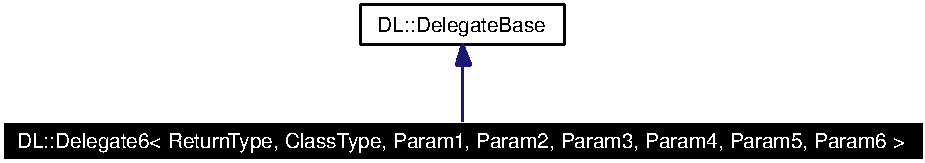
\includegraphics[width=239pt]{classDL_1_1Delegate6__inherit__graph}
\end{center}
\end{figure}
Collaboration diagram for DL::Delegate6$<$ Return\-Type, Class\-Type, Param1, Param2, Param3, Param4, Param5, Param6 $>$:\begin{figure}[H]
\begin{center}
\leavevmode
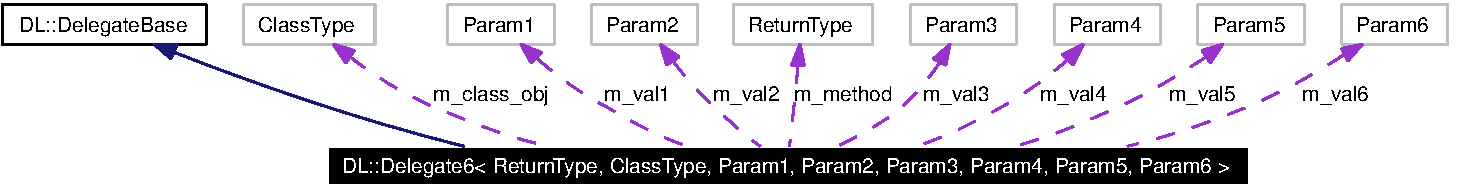
\includegraphics[width=369pt]{classDL_1_1Delegate6__coll__graph}
\end{center}
\end{figure}
\subsection*{Public Member Functions}
\begin{CompactItemize}
\item 
\hyperlink{classDL_1_1Delegate6_a0}{Delegate6} (Class\-Type $\ast$class\_\-obj, Return\-Type(Class\-Type::$\ast$method)(Param1, Param2, Param3, Param4, Param5, Param6), Param1 val1=Param1(), Param2 val2=Param2(), Param3 val3=Param3(), Param4 val4=Param4(), Param5 val5=Param5(), Param6 val6=Param6())
\item 
virtual \hyperlink{classDL_1_1Delegate6_a1}{$\sim$Delegate6} ()
\item 
void \hyperlink{classDL_1_1Delegate6_a2}{Invoke} ()
\item 
void \hyperlink{classDL_1_1Delegate6_a3}{Invoke} (Param1 val1, Param2 val2, Param3 val3, Param4 val4, Param5 val5, Param6 val6)
\end{CompactItemize}
\subsection*{Private Member Functions}
\begin{CompactItemize}
\item 
\hyperlink{classDL_1_1Delegate6_d0}{Delegate6} ()
\end{CompactItemize}
\subsection*{Private Attributes}
\begin{CompactItemize}
\item 
Class\-Type $\ast$ \hyperlink{classDL_1_1Delegate6_r0}{m\_\-class\_\-obj}
\item 
Return\-Type(Class\-Type::$\ast$ \hyperlink{classDL_1_1Delegate6_r1}{m\_\-method} )(Param1, Param2, Param3, Param4, Param5, Param6)
\item 
Param1 \hyperlink{classDL_1_1Delegate6_r2}{m\_\-val1}
\item 
Param2 \hyperlink{classDL_1_1Delegate6_r3}{m\_\-val2}
\item 
Param3 \hyperlink{classDL_1_1Delegate6_r4}{m\_\-val3}
\item 
Param4 \hyperlink{classDL_1_1Delegate6_r5}{m\_\-val4}
\item 
Param5 \hyperlink{classDL_1_1Delegate6_r6}{m\_\-val5}
\item 
Param6 \hyperlink{classDL_1_1Delegate6_r7}{m\_\-val6}
\end{CompactItemize}


\subsection{Detailed Description}
\subsubsection*{template$<$class Return\-Type, class Class\-Type, class Param1, class Param2, class Param3, class Param4, class Param5, class Param6$>$ class DL::Delegate6$<$ Return\-Type, Class\-Type, Param1, Param2, Param3, Param4, Param5, Param6 $>$}

Delegate for 6 Param



Definition at line 37 of file Delegate6.hpp.

\subsection{Constructor \& Destructor Documentation}
\hypertarget{classDL_1_1Delegate6_d0}{
\index{DL::Delegate6@{DL::Delegate6}!Delegate6@{Delegate6}}
\index{Delegate6@{Delegate6}!DL::Delegate6@{DL::Delegate6}}
\subsubsection[Delegate6]{\setlength{\rightskip}{0pt plus 5cm}template$<$class Return\-Type, class Class\-Type, class Param1, class Param2, class Param3, class Param4, class Param5, class Param6$>$ \hyperlink{classDL_1_1Delegate6}{DL::Delegate6}$<$ Return\-Type, Class\-Type, Param1, Param2, Param3, Param4, Param5, Param6 $>$::\hyperlink{classDL_1_1Delegate6}{Delegate6} ()\hspace{0.3cm}{\tt  \mbox{[}inline, private\mbox{]}}}}
\label{classDL_1_1Delegate6_d0}




Definition at line 47 of file Delegate6.hpp.\hypertarget{classDL_1_1Delegate6_a0}{
\index{DL::Delegate6@{DL::Delegate6}!Delegate6@{Delegate6}}
\index{Delegate6@{Delegate6}!DL::Delegate6@{DL::Delegate6}}
\subsubsection[Delegate6]{\setlength{\rightskip}{0pt plus 5cm}template$<$class Return\-Type, class Class\-Type, class Param1, class Param2, class Param3, class Param4, class Param5, class Param6$>$ \hyperlink{classDL_1_1Delegate6}{DL::Delegate6}$<$ Return\-Type, Class\-Type, Param1, Param2, Param3, Param4, Param5, Param6 $>$::\hyperlink{classDL_1_1Delegate6}{Delegate6} (Class\-Type $\ast$ {\em class\_\-obj}, Return\-Type(Class\-Type::$\ast$)(Param1, Param2, Param3, Param4, Param5, Param6) {\em method}, Param1 {\em val1} = {\tt Param1()}, Param2 {\em val2} = {\tt Param2()}, Param3 {\em val3} = {\tt Param3()}, Param4 {\em val4} = {\tt Param4()}, Param5 {\em val5} = {\tt Param5()}, Param6 {\em val6} = {\tt Param6()})\hspace{0.3cm}{\tt  \mbox{[}inline\mbox{]}}}}
\label{classDL_1_1Delegate6_a0}




Definition at line 49 of file Delegate6.hpp.

References DL::Delegate6$<$ Return\-Type, Class\-Type, Param1, Param2, Param3, Param4, Param5, Param6 $>$::m\_\-class\_\-obj, DL::Delegate6$<$ Return\-Type, Class\-Type, Param1, Param2, Param3, Param4, Param5, Param6 $>$::m\_\-method, DL::Delegate6$<$ Return\-Type, Class\-Type, Param1, Param2, Param3, Param4, Param5, Param6 $>$::m\_\-val1, DL::Delegate6$<$ Return\-Type, Class\-Type, Param1, Param2, Param3, Param4, Param5, Param6 $>$::m\_\-val2, DL::Delegate6$<$ Return\-Type, Class\-Type, Param1, Param2, Param3, Param4, Param5, Param6 $>$::m\_\-val3, DL::Delegate6$<$ Return\-Type, Class\-Type, Param1, Param2, Param3, Param4, Param5, Param6 $>$::m\_\-val4, DL::Delegate6$<$ Return\-Type, Class\-Type, Param1, Param2, Param3, Param4, Param5, Param6 $>$::m\_\-val5, and DL::Delegate6$<$ Return\-Type, Class\-Type, Param1, Param2, Param3, Param4, Param5, Param6 $>$::m\_\-val6.\hypertarget{classDL_1_1Delegate6_a1}{
\index{DL::Delegate6@{DL::Delegate6}!~Delegate6@{$\sim$Delegate6}}
\index{~Delegate6@{$\sim$Delegate6}!DL::Delegate6@{DL::Delegate6}}
\subsubsection[$\sim$Delegate6]{\setlength{\rightskip}{0pt plus 5cm}template$<$class Return\-Type, class Class\-Type, class Param1, class Param2, class Param3, class Param4, class Param5, class Param6$>$ virtual \hyperlink{classDL_1_1Delegate6}{DL::Delegate6}$<$ Return\-Type, Class\-Type, Param1, Param2, Param3, Param4, Param5, Param6 $>$::$\sim$\hyperlink{classDL_1_1Delegate6}{Delegate6} ()\hspace{0.3cm}{\tt  \mbox{[}inline, virtual\mbox{]}}}}
\label{classDL_1_1Delegate6_a1}




Definition at line 61 of file Delegate6.hpp.

\subsection{Member Function Documentation}
\hypertarget{classDL_1_1Delegate6_a3}{
\index{DL::Delegate6@{DL::Delegate6}!Invoke@{Invoke}}
\index{Invoke@{Invoke}!DL::Delegate6@{DL::Delegate6}}
\subsubsection[Invoke]{\setlength{\rightskip}{0pt plus 5cm}template$<$class Return\-Type, class Class\-Type, class Param1, class Param2, class Param3, class Param4, class Param5, class Param6$>$ void \hyperlink{classDL_1_1Delegate6}{DL::Delegate6}$<$ Return\-Type, Class\-Type, Param1, Param2, Param3, Param4, Param5, Param6 $>$::Invoke (Param1 {\em val1}, Param2 {\em val2}, Param3 {\em val3}, Param4 {\em val4}, Param5 {\em val5}, Param6 {\em val6})\hspace{0.3cm}{\tt  \mbox{[}inline\mbox{]}}}}
\label{classDL_1_1Delegate6_a3}




Definition at line 66 of file Delegate6.hpp.

References DL::Delegate6$<$ Return\-Type, Class\-Type, Param1, Param2, Param3, Param4, Param5, Param6 $>$::m\_\-class\_\-obj, and DL::Delegate6$<$ Return\-Type, Class\-Type, Param1, Param2, Param3, Param4, Param5, Param6 $>$::m\_\-method.\hypertarget{classDL_1_1Delegate6_a2}{
\index{DL::Delegate6@{DL::Delegate6}!Invoke@{Invoke}}
\index{Invoke@{Invoke}!DL::Delegate6@{DL::Delegate6}}
\subsubsection[Invoke]{\setlength{\rightskip}{0pt plus 5cm}template$<$class Return\-Type, class Class\-Type, class Param1, class Param2, class Param3, class Param4, class Param5, class Param6$>$ void \hyperlink{classDL_1_1Delegate6}{DL::Delegate6}$<$ Return\-Type, Class\-Type, Param1, Param2, Param3, Param4, Param5, Param6 $>$::Invoke ()\hspace{0.3cm}{\tt  \mbox{[}inline, virtual\mbox{]}}}}
\label{classDL_1_1Delegate6_a2}




Implements \hyperlink{classDL_1_1DelegateBase_a2}{DL::Delegate\-Base}.

Definition at line 62 of file Delegate6.hpp.

References DL::Delegate6$<$ Return\-Type, Class\-Type, Param1, Param2, Param3, Param4, Param5, Param6 $>$::m\_\-class\_\-obj, DL::Delegate6$<$ Return\-Type, Class\-Type, Param1, Param2, Param3, Param4, Param5, Param6 $>$::m\_\-method, DL::Delegate6$<$ Return\-Type, Class\-Type, Param1, Param2, Param3, Param4, Param5, Param6 $>$::m\_\-val1, DL::Delegate6$<$ Return\-Type, Class\-Type, Param1, Param2, Param3, Param4, Param5, Param6 $>$::m\_\-val2, DL::Delegate6$<$ Return\-Type, Class\-Type, Param1, Param2, Param3, Param4, Param5, Param6 $>$::m\_\-val3, DL::Delegate6$<$ Return\-Type, Class\-Type, Param1, Param2, Param3, Param4, Param5, Param6 $>$::m\_\-val4, DL::Delegate6$<$ Return\-Type, Class\-Type, Param1, Param2, Param3, Param4, Param5, Param6 $>$::m\_\-val5, and DL::Delegate6$<$ Return\-Type, Class\-Type, Param1, Param2, Param3, Param4, Param5, Param6 $>$::m\_\-val6.

\subsection{Member Data Documentation}
\hypertarget{classDL_1_1Delegate6_r0}{
\index{DL::Delegate6@{DL::Delegate6}!m_class_obj@{m\_\-class\_\-obj}}
\index{m_class_obj@{m\_\-class\_\-obj}!DL::Delegate6@{DL::Delegate6}}
\subsubsection[m\_\-class\_\-obj]{\setlength{\rightskip}{0pt plus 5cm}template$<$class Return\-Type, class Class\-Type, class Param1, class Param2, class Param3, class Param4, class Param5, class Param6$>$ Class\-Type$\ast$ \hyperlink{classDL_1_1Delegate6}{DL::Delegate6}$<$ Return\-Type, Class\-Type, Param1, Param2, Param3, Param4, Param5, Param6 $>$::\hyperlink{classDL_1_1Delegate6_r0}{m\_\-class\_\-obj}\hspace{0.3cm}{\tt  \mbox{[}private\mbox{]}}}}
\label{classDL_1_1Delegate6_r0}




Definition at line 39 of file Delegate6.hpp.

Referenced by DL::Delegate6$<$ Return\-Type, Class\-Type, Param1, Param2, Param3, Param4, Param5, Param6 $>$::Delegate6(), and DL::Delegate6$<$ Return\-Type, Class\-Type, Param1, Param2, Param3, Param4, Param5, Param6 $>$::Invoke().\hypertarget{classDL_1_1Delegate6_r1}{
\index{DL::Delegate6@{DL::Delegate6}!m_method@{m\_\-method}}
\index{m_method@{m\_\-method}!DL::Delegate6@{DL::Delegate6}}
\subsubsection[m\_\-method]{\setlength{\rightskip}{0pt plus 5cm}template$<$class Return\-Type, class Class\-Type, class Param1, class Param2, class Param3, class Param4, class Param5, class Param6$>$ Return\-Type(Class\-Type::$\ast$ \hyperlink{classDL_1_1Delegate6}{DL::Delegate6}$<$ Return\-Type, Class\-Type, Param1, Param2, Param3, Param4, Param5, Param6 $>$::\hyperlink{classDL_1_1Delegate6_r1}{m\_\-method})(Param1, Param2, Param3, Param4, Param5, Param6)\hspace{0.3cm}{\tt  \mbox{[}private\mbox{]}}}}
\label{classDL_1_1Delegate6_r1}




Referenced by DL::Delegate6$<$ Return\-Type, Class\-Type, Param1, Param2, Param3, Param4, Param5, Param6 $>$::Delegate6(), and DL::Delegate6$<$ Return\-Type, Class\-Type, Param1, Param2, Param3, Param4, Param5, Param6 $>$::Invoke().\hypertarget{classDL_1_1Delegate6_r2}{
\index{DL::Delegate6@{DL::Delegate6}!m_val1@{m\_\-val1}}
\index{m_val1@{m\_\-val1}!DL::Delegate6@{DL::Delegate6}}
\subsubsection[m\_\-val1]{\setlength{\rightskip}{0pt plus 5cm}template$<$class Return\-Type, class Class\-Type, class Param1, class Param2, class Param3, class Param4, class Param5, class Param6$>$ Param1 \hyperlink{classDL_1_1Delegate6}{DL::Delegate6}$<$ Return\-Type, Class\-Type, Param1, Param2, Param3, Param4, Param5, Param6 $>$::\hyperlink{classDL_1_1Delegate6_r2}{m\_\-val1}\hspace{0.3cm}{\tt  \mbox{[}private\mbox{]}}}}
\label{classDL_1_1Delegate6_r2}




Definition at line 41 of file Delegate6.hpp.

Referenced by DL::Delegate6$<$ Return\-Type, Class\-Type, Param1, Param2, Param3, Param4, Param5, Param6 $>$::Delegate6(), and DL::Delegate6$<$ Return\-Type, Class\-Type, Param1, Param2, Param3, Param4, Param5, Param6 $>$::Invoke().\hypertarget{classDL_1_1Delegate6_r3}{
\index{DL::Delegate6@{DL::Delegate6}!m_val2@{m\_\-val2}}
\index{m_val2@{m\_\-val2}!DL::Delegate6@{DL::Delegate6}}
\subsubsection[m\_\-val2]{\setlength{\rightskip}{0pt plus 5cm}template$<$class Return\-Type, class Class\-Type, class Param1, class Param2, class Param3, class Param4, class Param5, class Param6$>$ Param2 \hyperlink{classDL_1_1Delegate6}{DL::Delegate6}$<$ Return\-Type, Class\-Type, Param1, Param2, Param3, Param4, Param5, Param6 $>$::\hyperlink{classDL_1_1Delegate6_r3}{m\_\-val2}\hspace{0.3cm}{\tt  \mbox{[}private\mbox{]}}}}
\label{classDL_1_1Delegate6_r3}




Definition at line 42 of file Delegate6.hpp.

Referenced by DL::Delegate6$<$ Return\-Type, Class\-Type, Param1, Param2, Param3, Param4, Param5, Param6 $>$::Delegate6(), and DL::Delegate6$<$ Return\-Type, Class\-Type, Param1, Param2, Param3, Param4, Param5, Param6 $>$::Invoke().\hypertarget{classDL_1_1Delegate6_r4}{
\index{DL::Delegate6@{DL::Delegate6}!m_val3@{m\_\-val3}}
\index{m_val3@{m\_\-val3}!DL::Delegate6@{DL::Delegate6}}
\subsubsection[m\_\-val3]{\setlength{\rightskip}{0pt plus 5cm}template$<$class Return\-Type, class Class\-Type, class Param1, class Param2, class Param3, class Param4, class Param5, class Param6$>$ Param3 \hyperlink{classDL_1_1Delegate6}{DL::Delegate6}$<$ Return\-Type, Class\-Type, Param1, Param2, Param3, Param4, Param5, Param6 $>$::\hyperlink{classDL_1_1Delegate6_r4}{m\_\-val3}\hspace{0.3cm}{\tt  \mbox{[}private\mbox{]}}}}
\label{classDL_1_1Delegate6_r4}




Definition at line 43 of file Delegate6.hpp.

Referenced by DL::Delegate6$<$ Return\-Type, Class\-Type, Param1, Param2, Param3, Param4, Param5, Param6 $>$::Delegate6(), and DL::Delegate6$<$ Return\-Type, Class\-Type, Param1, Param2, Param3, Param4, Param5, Param6 $>$::Invoke().\hypertarget{classDL_1_1Delegate6_r5}{
\index{DL::Delegate6@{DL::Delegate6}!m_val4@{m\_\-val4}}
\index{m_val4@{m\_\-val4}!DL::Delegate6@{DL::Delegate6}}
\subsubsection[m\_\-val4]{\setlength{\rightskip}{0pt plus 5cm}template$<$class Return\-Type, class Class\-Type, class Param1, class Param2, class Param3, class Param4, class Param5, class Param6$>$ Param4 \hyperlink{classDL_1_1Delegate6}{DL::Delegate6}$<$ Return\-Type, Class\-Type, Param1, Param2, Param3, Param4, Param5, Param6 $>$::\hyperlink{classDL_1_1Delegate6_r5}{m\_\-val4}\hspace{0.3cm}{\tt  \mbox{[}private\mbox{]}}}}
\label{classDL_1_1Delegate6_r5}




Definition at line 44 of file Delegate6.hpp.

Referenced by DL::Delegate6$<$ Return\-Type, Class\-Type, Param1, Param2, Param3, Param4, Param5, Param6 $>$::Delegate6(), and DL::Delegate6$<$ Return\-Type, Class\-Type, Param1, Param2, Param3, Param4, Param5, Param6 $>$::Invoke().\hypertarget{classDL_1_1Delegate6_r6}{
\index{DL::Delegate6@{DL::Delegate6}!m_val5@{m\_\-val5}}
\index{m_val5@{m\_\-val5}!DL::Delegate6@{DL::Delegate6}}
\subsubsection[m\_\-val5]{\setlength{\rightskip}{0pt plus 5cm}template$<$class Return\-Type, class Class\-Type, class Param1, class Param2, class Param3, class Param4, class Param5, class Param6$>$ Param5 \hyperlink{classDL_1_1Delegate6}{DL::Delegate6}$<$ Return\-Type, Class\-Type, Param1, Param2, Param3, Param4, Param5, Param6 $>$::\hyperlink{classDL_1_1Delegate6_r6}{m\_\-val5}\hspace{0.3cm}{\tt  \mbox{[}private\mbox{]}}}}
\label{classDL_1_1Delegate6_r6}




Definition at line 45 of file Delegate6.hpp.

Referenced by DL::Delegate6$<$ Return\-Type, Class\-Type, Param1, Param2, Param3, Param4, Param5, Param6 $>$::Delegate6(), and DL::Delegate6$<$ Return\-Type, Class\-Type, Param1, Param2, Param3, Param4, Param5, Param6 $>$::Invoke().\hypertarget{classDL_1_1Delegate6_r7}{
\index{DL::Delegate6@{DL::Delegate6}!m_val6@{m\_\-val6}}
\index{m_val6@{m\_\-val6}!DL::Delegate6@{DL::Delegate6}}
\subsubsection[m\_\-val6]{\setlength{\rightskip}{0pt plus 5cm}template$<$class Return\-Type, class Class\-Type, class Param1, class Param2, class Param3, class Param4, class Param5, class Param6$>$ Param6 \hyperlink{classDL_1_1Delegate6}{DL::Delegate6}$<$ Return\-Type, Class\-Type, Param1, Param2, Param3, Param4, Param5, Param6 $>$::\hyperlink{classDL_1_1Delegate6_r7}{m\_\-val6}\hspace{0.3cm}{\tt  \mbox{[}private\mbox{]}}}}
\label{classDL_1_1Delegate6_r7}




Definition at line 46 of file Delegate6.hpp.

Referenced by DL::Delegate6$<$ Return\-Type, Class\-Type, Param1, Param2, Param3, Param4, Param5, Param6 $>$::Delegate6(), and DL::Delegate6$<$ Return\-Type, Class\-Type, Param1, Param2, Param3, Param4, Param5, Param6 $>$::Invoke().

The documentation for this class was generated from the following file:\begin{CompactItemize}
\item 
/data/callbackext/Delegate\-N/\hyperlink{Delegate6_8hpp}{Delegate6.hpp}\end{CompactItemize}

\hypertarget{classDL_1_1Delegate7}{
\section{DL::Delegate7$<$ Return\-Type, Class\-Type, Param1, Param2, Param3, Param4, Param5, Param6, Param7 $>$ Class Template Reference}
\label{classDL_1_1Delegate7}\index{DL::Delegate7@{DL::Delegate7}}
}
{\tt \#include $<$Delegate7.hpp$>$}

Inherits \hyperlink{classDL_1_1DelegateBase}{DL::Delegate\-Base}.

Inheritance diagram for DL::Delegate7$<$ Return\-Type, Class\-Type, Param1, Param2, Param3, Param4, Param5, Param6, Param7 $>$:\begin{figure}[H]
\begin{center}
\leavevmode
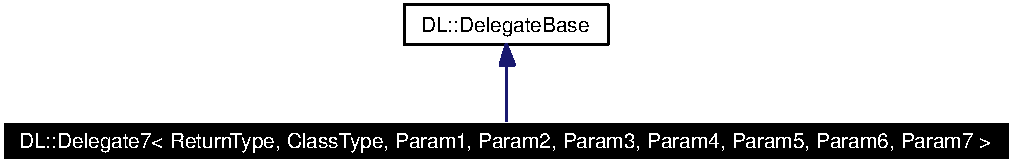
\includegraphics[width=260pt]{classDL_1_1Delegate7__inherit__graph}
\end{center}
\end{figure}
Collaboration diagram for DL::Delegate7$<$ Return\-Type, Class\-Type, Param1, Param2, Param3, Param4, Param5, Param6, Param7 $>$:\begin{figure}[H]
\begin{center}
\leavevmode
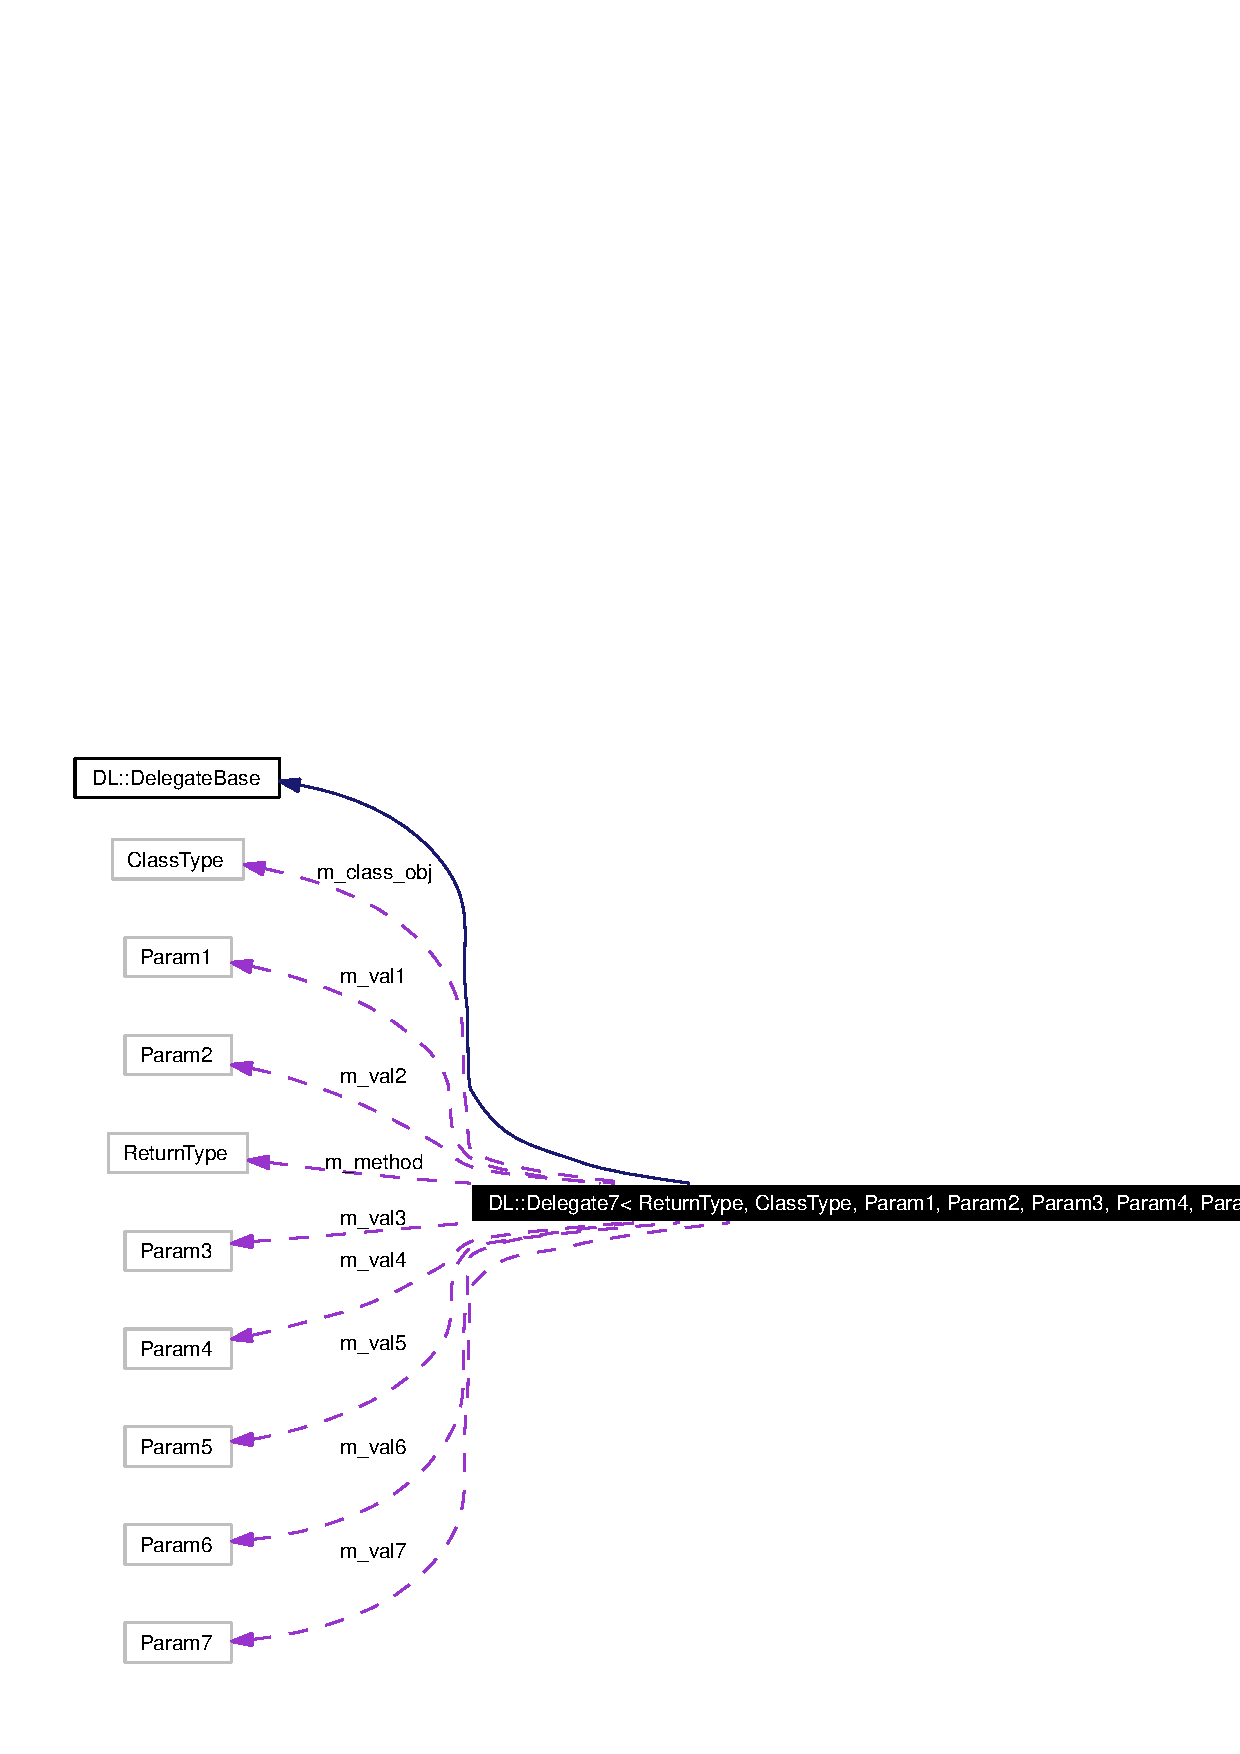
\includegraphics[width=355pt]{classDL_1_1Delegate7__coll__graph}
\end{center}
\end{figure}
\subsection*{Public Member Functions}
\begin{CompactItemize}
\item 
\hyperlink{classDL_1_1Delegate7_a0}{Delegate7} (Class\-Type $\ast$class\_\-obj, Return\-Type(Class\-Type::$\ast$method)(Param1, Param2, Param3, Param4, Param5, Param6, Param7), Param1 val1=Param1(), Param2 val2=Param2(), Param3 val3=Param3(), Param4 val4=Param4(), Param5 val5=Param5(), Param6 val6=Param6(), Param7 val7=Param7())
\item 
virtual \hyperlink{classDL_1_1Delegate7_a1}{$\sim$Delegate7} ()
\item 
void \hyperlink{classDL_1_1Delegate7_a2}{Invoke} ()
\item 
void \hyperlink{classDL_1_1Delegate7_a3}{Invoke} (Param1 val1, Param2 val2, Param3 val3, Param4 val4, Param5 val5, Param6 val6, Param7 val7)
\end{CompactItemize}
\subsection*{Private Member Functions}
\begin{CompactItemize}
\item 
\hyperlink{classDL_1_1Delegate7_d0}{Delegate7} ()
\end{CompactItemize}
\subsection*{Private Attributes}
\begin{CompactItemize}
\item 
Class\-Type $\ast$ \hyperlink{classDL_1_1Delegate7_r0}{m\_\-class\_\-obj}
\item 
Return\-Type(Class\-Type::$\ast$ \hyperlink{classDL_1_1Delegate7_r1}{m\_\-method} )(Param1, Param2, Param3, Param4, Param5, Param6, Param7)
\item 
Param1 \hyperlink{classDL_1_1Delegate7_r2}{m\_\-val1}
\item 
Param2 \hyperlink{classDL_1_1Delegate7_r3}{m\_\-val2}
\item 
Param3 \hyperlink{classDL_1_1Delegate7_r4}{m\_\-val3}
\item 
Param4 \hyperlink{classDL_1_1Delegate7_r5}{m\_\-val4}
\item 
Param5 \hyperlink{classDL_1_1Delegate7_r6}{m\_\-val5}
\item 
Param6 \hyperlink{classDL_1_1Delegate7_r7}{m\_\-val6}
\item 
Param7 \hyperlink{classDL_1_1Delegate7_r8}{m\_\-val7}
\end{CompactItemize}


\subsection{Detailed Description}
\subsubsection*{template$<$class Return\-Type, class Class\-Type, class Param1, class Param2, class Param3, class Param4, class Param5, class Param6, class Param7$>$ class DL::Delegate7$<$ Return\-Type, Class\-Type, Param1, Param2, Param3, Param4, Param5, Param6, Param7 $>$}

Delegate for 7 Param



Definition at line 38 of file Delegate7.hpp.

\subsection{Constructor \& Destructor Documentation}
\hypertarget{classDL_1_1Delegate7_d0}{
\index{DL::Delegate7@{DL::Delegate7}!Delegate7@{Delegate7}}
\index{Delegate7@{Delegate7}!DL::Delegate7@{DL::Delegate7}}
\subsubsection[Delegate7]{\setlength{\rightskip}{0pt plus 5cm}template$<$class Return\-Type, class Class\-Type, class Param1, class Param2, class Param3, class Param4, class Param5, class Param6, class Param7$>$ \hyperlink{classDL_1_1Delegate7}{DL::Delegate7}$<$ Return\-Type, Class\-Type, Param1, Param2, Param3, Param4, Param5, Param6, Param7 $>$::\hyperlink{classDL_1_1Delegate7}{Delegate7} ()\hspace{0.3cm}{\tt  \mbox{[}inline, private\mbox{]}}}}
\label{classDL_1_1Delegate7_d0}




Definition at line 49 of file Delegate7.hpp.\hypertarget{classDL_1_1Delegate7_a0}{
\index{DL::Delegate7@{DL::Delegate7}!Delegate7@{Delegate7}}
\index{Delegate7@{Delegate7}!DL::Delegate7@{DL::Delegate7}}
\subsubsection[Delegate7]{\setlength{\rightskip}{0pt plus 5cm}template$<$class Return\-Type, class Class\-Type, class Param1, class Param2, class Param3, class Param4, class Param5, class Param6, class Param7$>$ \hyperlink{classDL_1_1Delegate7}{DL::Delegate7}$<$ Return\-Type, Class\-Type, Param1, Param2, Param3, Param4, Param5, Param6, Param7 $>$::\hyperlink{classDL_1_1Delegate7}{Delegate7} (Class\-Type $\ast$ {\em class\_\-obj}, Return\-Type(Class\-Type::$\ast$)(Param1, Param2, Param3, Param4, Param5, Param6, Param7) {\em method}, Param1 {\em val1} = {\tt Param1()}, Param2 {\em val2} = {\tt Param2()}, Param3 {\em val3} = {\tt Param3()}, Param4 {\em val4} = {\tt Param4()}, Param5 {\em val5} = {\tt Param5()}, Param6 {\em val6} = {\tt Param6()}, Param7 {\em val7} = {\tt Param7()})\hspace{0.3cm}{\tt  \mbox{[}inline\mbox{]}}}}
\label{classDL_1_1Delegate7_a0}




Definition at line 51 of file Delegate7.hpp.

References DL::Delegate7$<$ Return\-Type, Class\-Type, Param1, Param2, Param3, Param4, Param5, Param6, Param7 $>$::m\_\-class\_\-obj, DL::Delegate7$<$ Return\-Type, Class\-Type, Param1, Param2, Param3, Param4, Param5, Param6, Param7 $>$::m\_\-method, DL::Delegate7$<$ Return\-Type, Class\-Type, Param1, Param2, Param3, Param4, Param5, Param6, Param7 $>$::m\_\-val1, DL::Delegate7$<$ Return\-Type, Class\-Type, Param1, Param2, Param3, Param4, Param5, Param6, Param7 $>$::m\_\-val2, DL::Delegate7$<$ Return\-Type, Class\-Type, Param1, Param2, Param3, Param4, Param5, Param6, Param7 $>$::m\_\-val3, DL::Delegate7$<$ Return\-Type, Class\-Type, Param1, Param2, Param3, Param4, Param5, Param6, Param7 $>$::m\_\-val4, DL::Delegate7$<$ Return\-Type, Class\-Type, Param1, Param2, Param3, Param4, Param5, Param6, Param7 $>$::m\_\-val5, DL::Delegate7$<$ Return\-Type, Class\-Type, Param1, Param2, Param3, Param4, Param5, Param6, Param7 $>$::m\_\-val6, and DL::Delegate7$<$ Return\-Type, Class\-Type, Param1, Param2, Param3, Param4, Param5, Param6, Param7 $>$::m\_\-val7.\hypertarget{classDL_1_1Delegate7_a1}{
\index{DL::Delegate7@{DL::Delegate7}!~Delegate7@{$\sim$Delegate7}}
\index{~Delegate7@{$\sim$Delegate7}!DL::Delegate7@{DL::Delegate7}}
\subsubsection[$\sim$Delegate7]{\setlength{\rightskip}{0pt plus 5cm}template$<$class Return\-Type, class Class\-Type, class Param1, class Param2, class Param3, class Param4, class Param5, class Param6, class Param7$>$ virtual \hyperlink{classDL_1_1Delegate7}{DL::Delegate7}$<$ Return\-Type, Class\-Type, Param1, Param2, Param3, Param4, Param5, Param6, Param7 $>$::$\sim$\hyperlink{classDL_1_1Delegate7}{Delegate7} ()\hspace{0.3cm}{\tt  \mbox{[}inline, virtual\mbox{]}}}}
\label{classDL_1_1Delegate7_a1}




Definition at line 65 of file Delegate7.hpp.

\subsection{Member Function Documentation}
\hypertarget{classDL_1_1Delegate7_a3}{
\index{DL::Delegate7@{DL::Delegate7}!Invoke@{Invoke}}
\index{Invoke@{Invoke}!DL::Delegate7@{DL::Delegate7}}
\subsubsection[Invoke]{\setlength{\rightskip}{0pt plus 5cm}template$<$class Return\-Type, class Class\-Type, class Param1, class Param2, class Param3, class Param4, class Param5, class Param6, class Param7$>$ void \hyperlink{classDL_1_1Delegate7}{DL::Delegate7}$<$ Return\-Type, Class\-Type, Param1, Param2, Param3, Param4, Param5, Param6, Param7 $>$::Invoke (Param1 {\em val1}, Param2 {\em val2}, Param3 {\em val3}, Param4 {\em val4}, Param5 {\em val5}, Param6 {\em val6}, Param7 {\em val7})\hspace{0.3cm}{\tt  \mbox{[}inline\mbox{]}}}}
\label{classDL_1_1Delegate7_a3}




Definition at line 70 of file Delegate7.hpp.

References DL::Delegate7$<$ Return\-Type, Class\-Type, Param1, Param2, Param3, Param4, Param5, Param6, Param7 $>$::m\_\-class\_\-obj, and DL::Delegate7$<$ Return\-Type, Class\-Type, Param1, Param2, Param3, Param4, Param5, Param6, Param7 $>$::m\_\-method.\hypertarget{classDL_1_1Delegate7_a2}{
\index{DL::Delegate7@{DL::Delegate7}!Invoke@{Invoke}}
\index{Invoke@{Invoke}!DL::Delegate7@{DL::Delegate7}}
\subsubsection[Invoke]{\setlength{\rightskip}{0pt plus 5cm}template$<$class Return\-Type, class Class\-Type, class Param1, class Param2, class Param3, class Param4, class Param5, class Param6, class Param7$>$ void \hyperlink{classDL_1_1Delegate7}{DL::Delegate7}$<$ Return\-Type, Class\-Type, Param1, Param2, Param3, Param4, Param5, Param6, Param7 $>$::Invoke ()\hspace{0.3cm}{\tt  \mbox{[}inline, virtual\mbox{]}}}}
\label{classDL_1_1Delegate7_a2}




Implements \hyperlink{classDL_1_1DelegateBase_a2}{DL::Delegate\-Base}.

Definition at line 66 of file Delegate7.hpp.

References DL::Delegate7$<$ Return\-Type, Class\-Type, Param1, Param2, Param3, Param4, Param5, Param6, Param7 $>$::m\_\-class\_\-obj, DL::Delegate7$<$ Return\-Type, Class\-Type, Param1, Param2, Param3, Param4, Param5, Param6, Param7 $>$::m\_\-method, DL::Delegate7$<$ Return\-Type, Class\-Type, Param1, Param2, Param3, Param4, Param5, Param6, Param7 $>$::m\_\-val1, DL::Delegate7$<$ Return\-Type, Class\-Type, Param1, Param2, Param3, Param4, Param5, Param6, Param7 $>$::m\_\-val2, DL::Delegate7$<$ Return\-Type, Class\-Type, Param1, Param2, Param3, Param4, Param5, Param6, Param7 $>$::m\_\-val3, DL::Delegate7$<$ Return\-Type, Class\-Type, Param1, Param2, Param3, Param4, Param5, Param6, Param7 $>$::m\_\-val4, DL::Delegate7$<$ Return\-Type, Class\-Type, Param1, Param2, Param3, Param4, Param5, Param6, Param7 $>$::m\_\-val5, DL::Delegate7$<$ Return\-Type, Class\-Type, Param1, Param2, Param3, Param4, Param5, Param6, Param7 $>$::m\_\-val6, and DL::Delegate7$<$ Return\-Type, Class\-Type, Param1, Param2, Param3, Param4, Param5, Param6, Param7 $>$::m\_\-val7.

\subsection{Member Data Documentation}
\hypertarget{classDL_1_1Delegate7_r0}{
\index{DL::Delegate7@{DL::Delegate7}!m_class_obj@{m\_\-class\_\-obj}}
\index{m_class_obj@{m\_\-class\_\-obj}!DL::Delegate7@{DL::Delegate7}}
\subsubsection[m\_\-class\_\-obj]{\setlength{\rightskip}{0pt plus 5cm}template$<$class Return\-Type, class Class\-Type, class Param1, class Param2, class Param3, class Param4, class Param5, class Param6, class Param7$>$ Class\-Type$\ast$ \hyperlink{classDL_1_1Delegate7}{DL::Delegate7}$<$ Return\-Type, Class\-Type, Param1, Param2, Param3, Param4, Param5, Param6, Param7 $>$::\hyperlink{classDL_1_1Delegate7_r0}{m\_\-class\_\-obj}\hspace{0.3cm}{\tt  \mbox{[}private\mbox{]}}}}
\label{classDL_1_1Delegate7_r0}




Definition at line 40 of file Delegate7.hpp.

Referenced by DL::Delegate7$<$ Return\-Type, Class\-Type, Param1, Param2, Param3, Param4, Param5, Param6, Param7 $>$::Delegate7(), and DL::Delegate7$<$ Return\-Type, Class\-Type, Param1, Param2, Param3, Param4, Param5, Param6, Param7 $>$::Invoke().\hypertarget{classDL_1_1Delegate7_r1}{
\index{DL::Delegate7@{DL::Delegate7}!m_method@{m\_\-method}}
\index{m_method@{m\_\-method}!DL::Delegate7@{DL::Delegate7}}
\subsubsection[m\_\-method]{\setlength{\rightskip}{0pt plus 5cm}template$<$class Return\-Type, class Class\-Type, class Param1, class Param2, class Param3, class Param4, class Param5, class Param6, class Param7$>$ Return\-Type(Class\-Type::$\ast$ \hyperlink{classDL_1_1Delegate7}{DL::Delegate7}$<$ Return\-Type, Class\-Type, Param1, Param2, Param3, Param4, Param5, Param6, Param7 $>$::\hyperlink{classDL_1_1Delegate7_r1}{m\_\-method})(Param1, Param2, Param3, Param4, Param5, Param6, Param7)\hspace{0.3cm}{\tt  \mbox{[}private\mbox{]}}}}
\label{classDL_1_1Delegate7_r1}




Referenced by DL::Delegate7$<$ Return\-Type, Class\-Type, Param1, Param2, Param3, Param4, Param5, Param6, Param7 $>$::Delegate7(), and DL::Delegate7$<$ Return\-Type, Class\-Type, Param1, Param2, Param3, Param4, Param5, Param6, Param7 $>$::Invoke().\hypertarget{classDL_1_1Delegate7_r2}{
\index{DL::Delegate7@{DL::Delegate7}!m_val1@{m\_\-val1}}
\index{m_val1@{m\_\-val1}!DL::Delegate7@{DL::Delegate7}}
\subsubsection[m\_\-val1]{\setlength{\rightskip}{0pt plus 5cm}template$<$class Return\-Type, class Class\-Type, class Param1, class Param2, class Param3, class Param4, class Param5, class Param6, class Param7$>$ Param1 \hyperlink{classDL_1_1Delegate7}{DL::Delegate7}$<$ Return\-Type, Class\-Type, Param1, Param2, Param3, Param4, Param5, Param6, Param7 $>$::\hyperlink{classDL_1_1Delegate7_r2}{m\_\-val1}\hspace{0.3cm}{\tt  \mbox{[}private\mbox{]}}}}
\label{classDL_1_1Delegate7_r2}




Definition at line 42 of file Delegate7.hpp.

Referenced by DL::Delegate7$<$ Return\-Type, Class\-Type, Param1, Param2, Param3, Param4, Param5, Param6, Param7 $>$::Delegate7(), and DL::Delegate7$<$ Return\-Type, Class\-Type, Param1, Param2, Param3, Param4, Param5, Param6, Param7 $>$::Invoke().\hypertarget{classDL_1_1Delegate7_r3}{
\index{DL::Delegate7@{DL::Delegate7}!m_val2@{m\_\-val2}}
\index{m_val2@{m\_\-val2}!DL::Delegate7@{DL::Delegate7}}
\subsubsection[m\_\-val2]{\setlength{\rightskip}{0pt plus 5cm}template$<$class Return\-Type, class Class\-Type, class Param1, class Param2, class Param3, class Param4, class Param5, class Param6, class Param7$>$ Param2 \hyperlink{classDL_1_1Delegate7}{DL::Delegate7}$<$ Return\-Type, Class\-Type, Param1, Param2, Param3, Param4, Param5, Param6, Param7 $>$::\hyperlink{classDL_1_1Delegate7_r3}{m\_\-val2}\hspace{0.3cm}{\tt  \mbox{[}private\mbox{]}}}}
\label{classDL_1_1Delegate7_r3}




Definition at line 43 of file Delegate7.hpp.

Referenced by DL::Delegate7$<$ Return\-Type, Class\-Type, Param1, Param2, Param3, Param4, Param5, Param6, Param7 $>$::Delegate7(), and DL::Delegate7$<$ Return\-Type, Class\-Type, Param1, Param2, Param3, Param4, Param5, Param6, Param7 $>$::Invoke().\hypertarget{classDL_1_1Delegate7_r4}{
\index{DL::Delegate7@{DL::Delegate7}!m_val3@{m\_\-val3}}
\index{m_val3@{m\_\-val3}!DL::Delegate7@{DL::Delegate7}}
\subsubsection[m\_\-val3]{\setlength{\rightskip}{0pt plus 5cm}template$<$class Return\-Type, class Class\-Type, class Param1, class Param2, class Param3, class Param4, class Param5, class Param6, class Param7$>$ Param3 \hyperlink{classDL_1_1Delegate7}{DL::Delegate7}$<$ Return\-Type, Class\-Type, Param1, Param2, Param3, Param4, Param5, Param6, Param7 $>$::\hyperlink{classDL_1_1Delegate7_r4}{m\_\-val3}\hspace{0.3cm}{\tt  \mbox{[}private\mbox{]}}}}
\label{classDL_1_1Delegate7_r4}




Definition at line 44 of file Delegate7.hpp.

Referenced by DL::Delegate7$<$ Return\-Type, Class\-Type, Param1, Param2, Param3, Param4, Param5, Param6, Param7 $>$::Delegate7(), and DL::Delegate7$<$ Return\-Type, Class\-Type, Param1, Param2, Param3, Param4, Param5, Param6, Param7 $>$::Invoke().\hypertarget{classDL_1_1Delegate7_r5}{
\index{DL::Delegate7@{DL::Delegate7}!m_val4@{m\_\-val4}}
\index{m_val4@{m\_\-val4}!DL::Delegate7@{DL::Delegate7}}
\subsubsection[m\_\-val4]{\setlength{\rightskip}{0pt plus 5cm}template$<$class Return\-Type, class Class\-Type, class Param1, class Param2, class Param3, class Param4, class Param5, class Param6, class Param7$>$ Param4 \hyperlink{classDL_1_1Delegate7}{DL::Delegate7}$<$ Return\-Type, Class\-Type, Param1, Param2, Param3, Param4, Param5, Param6, Param7 $>$::\hyperlink{classDL_1_1Delegate7_r5}{m\_\-val4}\hspace{0.3cm}{\tt  \mbox{[}private\mbox{]}}}}
\label{classDL_1_1Delegate7_r5}




Definition at line 45 of file Delegate7.hpp.

Referenced by DL::Delegate7$<$ Return\-Type, Class\-Type, Param1, Param2, Param3, Param4, Param5, Param6, Param7 $>$::Delegate7(), and DL::Delegate7$<$ Return\-Type, Class\-Type, Param1, Param2, Param3, Param4, Param5, Param6, Param7 $>$::Invoke().\hypertarget{classDL_1_1Delegate7_r6}{
\index{DL::Delegate7@{DL::Delegate7}!m_val5@{m\_\-val5}}
\index{m_val5@{m\_\-val5}!DL::Delegate7@{DL::Delegate7}}
\subsubsection[m\_\-val5]{\setlength{\rightskip}{0pt plus 5cm}template$<$class Return\-Type, class Class\-Type, class Param1, class Param2, class Param3, class Param4, class Param5, class Param6, class Param7$>$ Param5 \hyperlink{classDL_1_1Delegate7}{DL::Delegate7}$<$ Return\-Type, Class\-Type, Param1, Param2, Param3, Param4, Param5, Param6, Param7 $>$::\hyperlink{classDL_1_1Delegate7_r6}{m\_\-val5}\hspace{0.3cm}{\tt  \mbox{[}private\mbox{]}}}}
\label{classDL_1_1Delegate7_r6}




Definition at line 46 of file Delegate7.hpp.

Referenced by DL::Delegate7$<$ Return\-Type, Class\-Type, Param1, Param2, Param3, Param4, Param5, Param6, Param7 $>$::Delegate7(), and DL::Delegate7$<$ Return\-Type, Class\-Type, Param1, Param2, Param3, Param4, Param5, Param6, Param7 $>$::Invoke().\hypertarget{classDL_1_1Delegate7_r7}{
\index{DL::Delegate7@{DL::Delegate7}!m_val6@{m\_\-val6}}
\index{m_val6@{m\_\-val6}!DL::Delegate7@{DL::Delegate7}}
\subsubsection[m\_\-val6]{\setlength{\rightskip}{0pt plus 5cm}template$<$class Return\-Type, class Class\-Type, class Param1, class Param2, class Param3, class Param4, class Param5, class Param6, class Param7$>$ Param6 \hyperlink{classDL_1_1Delegate7}{DL::Delegate7}$<$ Return\-Type, Class\-Type, Param1, Param2, Param3, Param4, Param5, Param6, Param7 $>$::\hyperlink{classDL_1_1Delegate7_r7}{m\_\-val6}\hspace{0.3cm}{\tt  \mbox{[}private\mbox{]}}}}
\label{classDL_1_1Delegate7_r7}




Definition at line 47 of file Delegate7.hpp.

Referenced by DL::Delegate7$<$ Return\-Type, Class\-Type, Param1, Param2, Param3, Param4, Param5, Param6, Param7 $>$::Delegate7(), and DL::Delegate7$<$ Return\-Type, Class\-Type, Param1, Param2, Param3, Param4, Param5, Param6, Param7 $>$::Invoke().\hypertarget{classDL_1_1Delegate7_r8}{
\index{DL::Delegate7@{DL::Delegate7}!m_val7@{m\_\-val7}}
\index{m_val7@{m\_\-val7}!DL::Delegate7@{DL::Delegate7}}
\subsubsection[m\_\-val7]{\setlength{\rightskip}{0pt plus 5cm}template$<$class Return\-Type, class Class\-Type, class Param1, class Param2, class Param3, class Param4, class Param5, class Param6, class Param7$>$ Param7 \hyperlink{classDL_1_1Delegate7}{DL::Delegate7}$<$ Return\-Type, Class\-Type, Param1, Param2, Param3, Param4, Param5, Param6, Param7 $>$::\hyperlink{classDL_1_1Delegate7_r8}{m\_\-val7}\hspace{0.3cm}{\tt  \mbox{[}private\mbox{]}}}}
\label{classDL_1_1Delegate7_r8}




Definition at line 48 of file Delegate7.hpp.

Referenced by DL::Delegate7$<$ Return\-Type, Class\-Type, Param1, Param2, Param3, Param4, Param5, Param6, Param7 $>$::Delegate7(), and DL::Delegate7$<$ Return\-Type, Class\-Type, Param1, Param2, Param3, Param4, Param5, Param6, Param7 $>$::Invoke().

The documentation for this class was generated from the following file:\begin{CompactItemize}
\item 
/data/callbackext/Delegate\-N/\hyperlink{Delegate7_8hpp}{Delegate7.hpp}\end{CompactItemize}

\hypertarget{classDL_1_1Delegate8}{
\section{DL::Delegate8$<$ Return\-Type, Class\-Type, Param1, Param2, Param3, Param4, Param5, Param6, Param7, Param8 $>$ Class Template Reference}
\label{classDL_1_1Delegate8}\index{DL::Delegate8@{DL::Delegate8}}
}
{\tt \#include $<$Delegate8.hpp$>$}

Inherits \hyperlink{classDL_1_1DelegateBase}{DL::Delegate\-Base}.

Inheritance diagram for DL::Delegate8$<$ Return\-Type, Class\-Type, Param1, Param2, Param3, Param4, Param5, Param6, Param7, Param8 $>$:\begin{figure}[H]
\begin{center}
\leavevmode
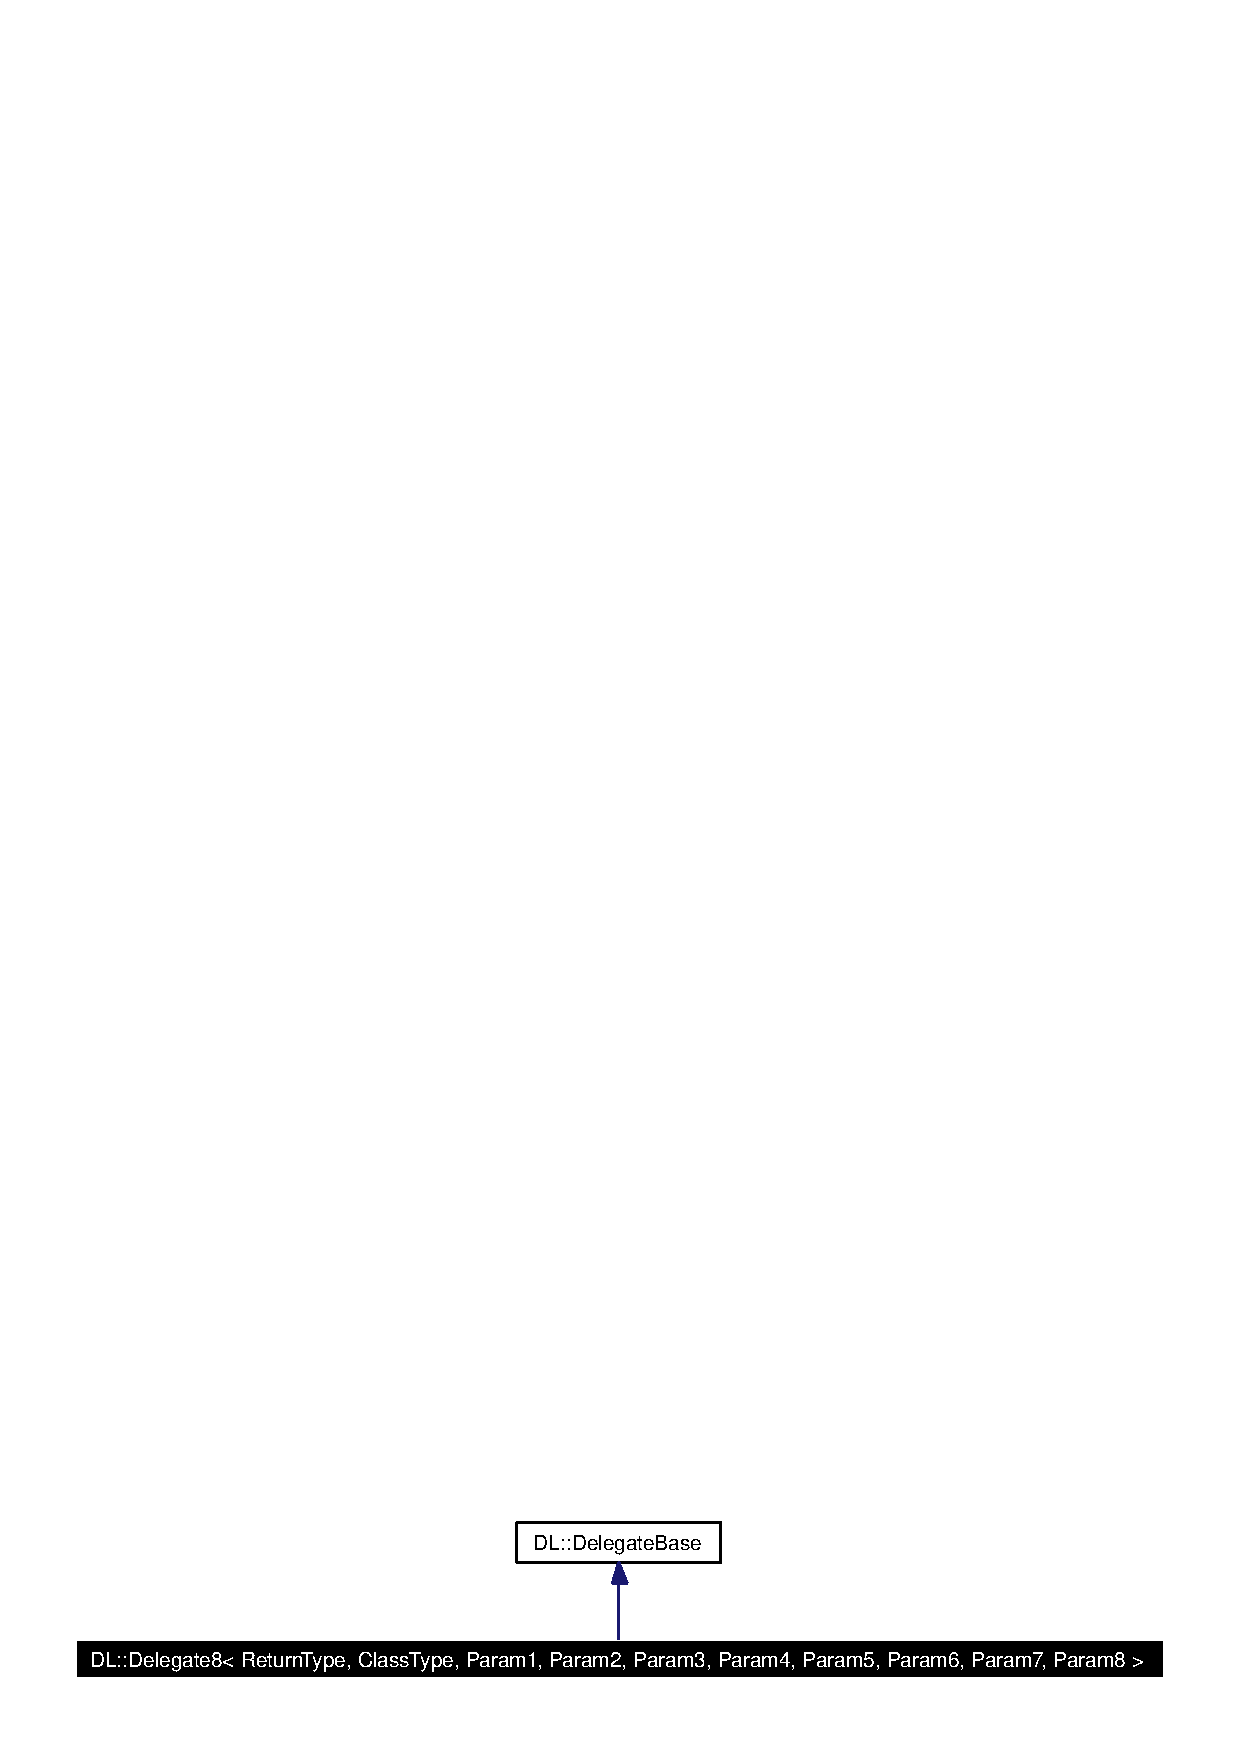
\includegraphics[width=279pt]{classDL_1_1Delegate8__inherit__graph}
\end{center}
\end{figure}
Collaboration diagram for DL::Delegate8$<$ Return\-Type, Class\-Type, Param1, Param2, Param3, Param4, Param5, Param6, Param7, Param8 $>$:\begin{figure}[H]
\begin{center}
\leavevmode
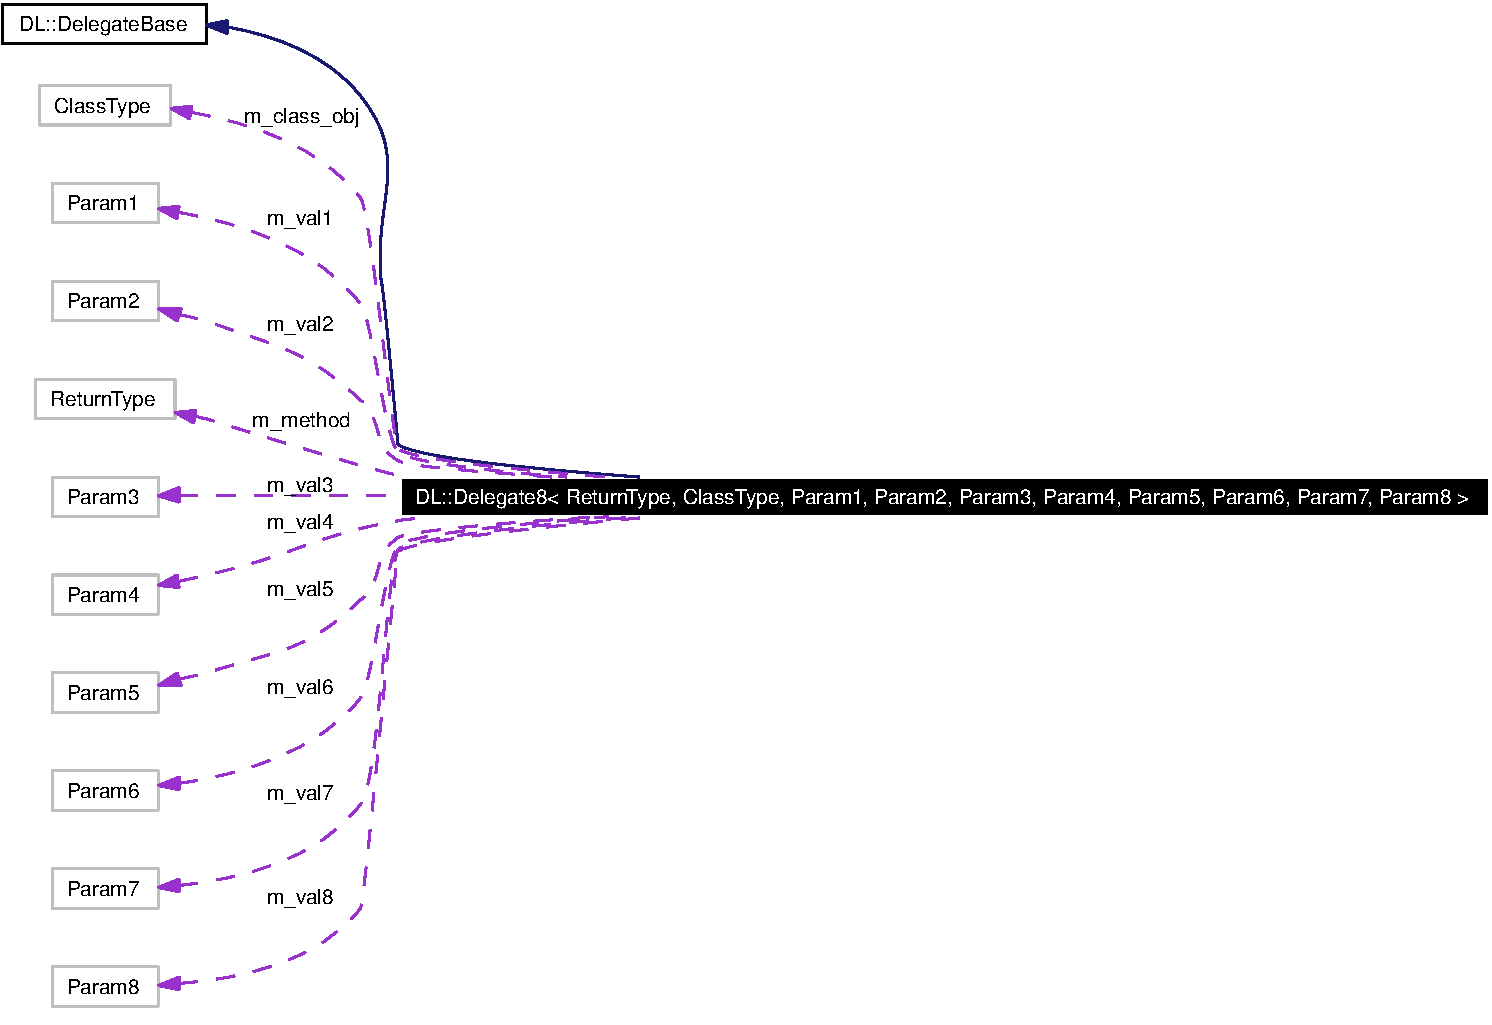
\includegraphics[width=375pt]{classDL_1_1Delegate8__coll__graph}
\end{center}
\end{figure}
\subsection*{Public Member Functions}
\begin{CompactItemize}
\item 
\hyperlink{classDL_1_1Delegate8_a0}{Delegate8} (Class\-Type $\ast$class\_\-obj, Return\-Type(Class\-Type::$\ast$method)(Param1, Param2, Param3, Param4, Param5, Param6, Param7, Param8), Param1 val1=Param1(), Param2 val2=Param2(), Param3 val3=Param3(), Param4 val4=Param4(), Param5 val5=Param5(), Param6 val6=Param6(), Param7 val7=Param7(), Param8 val8=Param8())
\item 
virtual \hyperlink{classDL_1_1Delegate8_a1}{$\sim$Delegate8} ()
\item 
void \hyperlink{classDL_1_1Delegate8_a2}{Invoke} ()
\item 
void \hyperlink{classDL_1_1Delegate8_a3}{Invoke} (Param1 val1, Param2 val2, Param3 val3, Param4 val4, Param5 val5, Param6 val6, Param7 val7, Param8 val8)
\end{CompactItemize}
\subsection*{Private Member Functions}
\begin{CompactItemize}
\item 
\hyperlink{classDL_1_1Delegate8_d0}{Delegate8} ()
\end{CompactItemize}
\subsection*{Private Attributes}
\begin{CompactItemize}
\item 
Class\-Type $\ast$ \hyperlink{classDL_1_1Delegate8_r0}{m\_\-class\_\-obj}
\item 
Return\-Type(Class\-Type::$\ast$ \hyperlink{classDL_1_1Delegate8_r1}{m\_\-method} )(Param1, Param2, Param3, Param4, Param5, Param6, Param7, Param8)
\item 
Param1 \hyperlink{classDL_1_1Delegate8_r2}{m\_\-val1}
\item 
Param2 \hyperlink{classDL_1_1Delegate8_r3}{m\_\-val2}
\item 
Param3 \hyperlink{classDL_1_1Delegate8_r4}{m\_\-val3}
\item 
Param4 \hyperlink{classDL_1_1Delegate8_r5}{m\_\-val4}
\item 
Param5 \hyperlink{classDL_1_1Delegate8_r6}{m\_\-val5}
\item 
Param6 \hyperlink{classDL_1_1Delegate8_r7}{m\_\-val6}
\item 
Param7 \hyperlink{classDL_1_1Delegate8_r8}{m\_\-val7}
\item 
Param8 \hyperlink{classDL_1_1Delegate8_r9}{m\_\-val8}
\end{CompactItemize}


\subsection{Detailed Description}
\subsubsection*{template$<$class Return\-Type, class Class\-Type, class Param1, class Param2, class Param3, class Param4, class Param5, class Param6, class Param7, class Param8$>$ class DL::Delegate8$<$ Return\-Type, Class\-Type, Param1, Param2, Param3, Param4, Param5, Param6, Param7, Param8 $>$}

Delegate for 8 Param



Definition at line 39 of file Delegate8.hpp.

\subsection{Constructor \& Destructor Documentation}
\hypertarget{classDL_1_1Delegate8_d0}{
\index{DL::Delegate8@{DL::Delegate8}!Delegate8@{Delegate8}}
\index{Delegate8@{Delegate8}!DL::Delegate8@{DL::Delegate8}}
\subsubsection[Delegate8]{\setlength{\rightskip}{0pt plus 5cm}template$<$class Return\-Type, class Class\-Type, class Param1, class Param2, class Param3, class Param4, class Param5, class Param6, class Param7, class Param8$>$ \hyperlink{classDL_1_1Delegate8}{DL::Delegate8}$<$ Return\-Type, Class\-Type, Param1, Param2, Param3, Param4, Param5, Param6, Param7, Param8 $>$::\hyperlink{classDL_1_1Delegate8}{Delegate8} ()\hspace{0.3cm}{\tt  \mbox{[}inline, private\mbox{]}}}}
\label{classDL_1_1Delegate8_d0}




Definition at line 51 of file Delegate8.hpp.\hypertarget{classDL_1_1Delegate8_a0}{
\index{DL::Delegate8@{DL::Delegate8}!Delegate8@{Delegate8}}
\index{Delegate8@{Delegate8}!DL::Delegate8@{DL::Delegate8}}
\subsubsection[Delegate8]{\setlength{\rightskip}{0pt plus 5cm}template$<$class Return\-Type, class Class\-Type, class Param1, class Param2, class Param3, class Param4, class Param5, class Param6, class Param7, class Param8$>$ \hyperlink{classDL_1_1Delegate8}{DL::Delegate8}$<$ Return\-Type, Class\-Type, Param1, Param2, Param3, Param4, Param5, Param6, Param7, Param8 $>$::\hyperlink{classDL_1_1Delegate8}{Delegate8} (Class\-Type $\ast$ {\em class\_\-obj}, Return\-Type(Class\-Type::$\ast$)(Param1, Param2, Param3, Param4, Param5, Param6, Param7, Param8) {\em method}, Param1 {\em val1} = {\tt Param1()}, Param2 {\em val2} = {\tt Param2()}, Param3 {\em val3} = {\tt Param3()}, Param4 {\em val4} = {\tt Param4()}, Param5 {\em val5} = {\tt Param5()}, Param6 {\em val6} = {\tt Param6()}, Param7 {\em val7} = {\tt Param7()}, Param8 {\em val8} = {\tt Param8()})\hspace{0.3cm}{\tt  \mbox{[}inline\mbox{]}}}}
\label{classDL_1_1Delegate8_a0}




Definition at line 53 of file Delegate8.hpp.

References DL::Delegate8$<$ Return\-Type, Class\-Type, Param1, Param2, Param3, Param4, Param5, Param6, Param7, Param8 $>$::m\_\-class\_\-obj, DL::Delegate8$<$ Return\-Type, Class\-Type, Param1, Param2, Param3, Param4, Param5, Param6, Param7, Param8 $>$::m\_\-method, DL::Delegate8$<$ Return\-Type, Class\-Type, Param1, Param2, Param3, Param4, Param5, Param6, Param7, Param8 $>$::m\_\-val1, DL::Delegate8$<$ Return\-Type, Class\-Type, Param1, Param2, Param3, Param4, Param5, Param6, Param7, Param8 $>$::m\_\-val2, DL::Delegate8$<$ Return\-Type, Class\-Type, Param1, Param2, Param3, Param4, Param5, Param6, Param7, Param8 $>$::m\_\-val3, DL::Delegate8$<$ Return\-Type, Class\-Type, Param1, Param2, Param3, Param4, Param5, Param6, Param7, Param8 $>$::m\_\-val4, DL::Delegate8$<$ Return\-Type, Class\-Type, Param1, Param2, Param3, Param4, Param5, Param6, Param7, Param8 $>$::m\_\-val5, DL::Delegate8$<$ Return\-Type, Class\-Type, Param1, Param2, Param3, Param4, Param5, Param6, Param7, Param8 $>$::m\_\-val6, DL::Delegate8$<$ Return\-Type, Class\-Type, Param1, Param2, Param3, Param4, Param5, Param6, Param7, Param8 $>$::m\_\-val7, and DL::Delegate8$<$ Return\-Type, Class\-Type, Param1, Param2, Param3, Param4, Param5, Param6, Param7, Param8 $>$::m\_\-val8.\hypertarget{classDL_1_1Delegate8_a1}{
\index{DL::Delegate8@{DL::Delegate8}!~Delegate8@{$\sim$Delegate8}}
\index{~Delegate8@{$\sim$Delegate8}!DL::Delegate8@{DL::Delegate8}}
\subsubsection[$\sim$Delegate8]{\setlength{\rightskip}{0pt plus 5cm}template$<$class Return\-Type, class Class\-Type, class Param1, class Param2, class Param3, class Param4, class Param5, class Param6, class Param7, class Param8$>$ virtual \hyperlink{classDL_1_1Delegate8}{DL::Delegate8}$<$ Return\-Type, Class\-Type, Param1, Param2, Param3, Param4, Param5, Param6, Param7, Param8 $>$::$\sim$\hyperlink{classDL_1_1Delegate8}{Delegate8} ()\hspace{0.3cm}{\tt  \mbox{[}inline, virtual\mbox{]}}}}
\label{classDL_1_1Delegate8_a1}




Definition at line 68 of file Delegate8.hpp.

\subsection{Member Function Documentation}
\hypertarget{classDL_1_1Delegate8_a3}{
\index{DL::Delegate8@{DL::Delegate8}!Invoke@{Invoke}}
\index{Invoke@{Invoke}!DL::Delegate8@{DL::Delegate8}}
\subsubsection[Invoke]{\setlength{\rightskip}{0pt plus 5cm}template$<$class Return\-Type, class Class\-Type, class Param1, class Param2, class Param3, class Param4, class Param5, class Param6, class Param7, class Param8$>$ void \hyperlink{classDL_1_1Delegate8}{DL::Delegate8}$<$ Return\-Type, Class\-Type, Param1, Param2, Param3, Param4, Param5, Param6, Param7, Param8 $>$::Invoke (Param1 {\em val1}, Param2 {\em val2}, Param3 {\em val3}, Param4 {\em val4}, Param5 {\em val5}, Param6 {\em val6}, Param7 {\em val7}, Param8 {\em val8})\hspace{0.3cm}{\tt  \mbox{[}inline\mbox{]}}}}
\label{classDL_1_1Delegate8_a3}




Definition at line 73 of file Delegate8.hpp.

References DL::Delegate8$<$ Return\-Type, Class\-Type, Param1, Param2, Param3, Param4, Param5, Param6, Param7, Param8 $>$::m\_\-class\_\-obj, and DL::Delegate8$<$ Return\-Type, Class\-Type, Param1, Param2, Param3, Param4, Param5, Param6, Param7, Param8 $>$::m\_\-method.\hypertarget{classDL_1_1Delegate8_a2}{
\index{DL::Delegate8@{DL::Delegate8}!Invoke@{Invoke}}
\index{Invoke@{Invoke}!DL::Delegate8@{DL::Delegate8}}
\subsubsection[Invoke]{\setlength{\rightskip}{0pt plus 5cm}template$<$class Return\-Type, class Class\-Type, class Param1, class Param2, class Param3, class Param4, class Param5, class Param6, class Param7, class Param8$>$ void \hyperlink{classDL_1_1Delegate8}{DL::Delegate8}$<$ Return\-Type, Class\-Type, Param1, Param2, Param3, Param4, Param5, Param6, Param7, Param8 $>$::Invoke ()\hspace{0.3cm}{\tt  \mbox{[}inline, virtual\mbox{]}}}}
\label{classDL_1_1Delegate8_a2}




Implements \hyperlink{classDL_1_1DelegateBase_a2}{DL::Delegate\-Base}.

Definition at line 69 of file Delegate8.hpp.

References DL::Delegate8$<$ Return\-Type, Class\-Type, Param1, Param2, Param3, Param4, Param5, Param6, Param7, Param8 $>$::m\_\-class\_\-obj, DL::Delegate8$<$ Return\-Type, Class\-Type, Param1, Param2, Param3, Param4, Param5, Param6, Param7, Param8 $>$::m\_\-method, DL::Delegate8$<$ Return\-Type, Class\-Type, Param1, Param2, Param3, Param4, Param5, Param6, Param7, Param8 $>$::m\_\-val1, DL::Delegate8$<$ Return\-Type, Class\-Type, Param1, Param2, Param3, Param4, Param5, Param6, Param7, Param8 $>$::m\_\-val2, DL::Delegate8$<$ Return\-Type, Class\-Type, Param1, Param2, Param3, Param4, Param5, Param6, Param7, Param8 $>$::m\_\-val3, DL::Delegate8$<$ Return\-Type, Class\-Type, Param1, Param2, Param3, Param4, Param5, Param6, Param7, Param8 $>$::m\_\-val4, DL::Delegate8$<$ Return\-Type, Class\-Type, Param1, Param2, Param3, Param4, Param5, Param6, Param7, Param8 $>$::m\_\-val5, DL::Delegate8$<$ Return\-Type, Class\-Type, Param1, Param2, Param3, Param4, Param5, Param6, Param7, Param8 $>$::m\_\-val6, DL::Delegate8$<$ Return\-Type, Class\-Type, Param1, Param2, Param3, Param4, Param5, Param6, Param7, Param8 $>$::m\_\-val7, and DL::Delegate8$<$ Return\-Type, Class\-Type, Param1, Param2, Param3, Param4, Param5, Param6, Param7, Param8 $>$::m\_\-val8.

\subsection{Member Data Documentation}
\hypertarget{classDL_1_1Delegate8_r0}{
\index{DL::Delegate8@{DL::Delegate8}!m_class_obj@{m\_\-class\_\-obj}}
\index{m_class_obj@{m\_\-class\_\-obj}!DL::Delegate8@{DL::Delegate8}}
\subsubsection[m\_\-class\_\-obj]{\setlength{\rightskip}{0pt plus 5cm}template$<$class Return\-Type, class Class\-Type, class Param1, class Param2, class Param3, class Param4, class Param5, class Param6, class Param7, class Param8$>$ Class\-Type$\ast$ \hyperlink{classDL_1_1Delegate8}{DL::Delegate8}$<$ Return\-Type, Class\-Type, Param1, Param2, Param3, Param4, Param5, Param6, Param7, Param8 $>$::\hyperlink{classDL_1_1Delegate8_r0}{m\_\-class\_\-obj}\hspace{0.3cm}{\tt  \mbox{[}private\mbox{]}}}}
\label{classDL_1_1Delegate8_r0}




Definition at line 41 of file Delegate8.hpp.

Referenced by DL::Delegate8$<$ Return\-Type, Class\-Type, Param1, Param2, Param3, Param4, Param5, Param6, Param7, Param8 $>$::Delegate8(), and DL::Delegate8$<$ Return\-Type, Class\-Type, Param1, Param2, Param3, Param4, Param5, Param6, Param7, Param8 $>$::Invoke().\hypertarget{classDL_1_1Delegate8_r1}{
\index{DL::Delegate8@{DL::Delegate8}!m_method@{m\_\-method}}
\index{m_method@{m\_\-method}!DL::Delegate8@{DL::Delegate8}}
\subsubsection[m\_\-method]{\setlength{\rightskip}{0pt plus 5cm}template$<$class Return\-Type, class Class\-Type, class Param1, class Param2, class Param3, class Param4, class Param5, class Param6, class Param7, class Param8$>$ Return\-Type(Class\-Type::$\ast$ \hyperlink{classDL_1_1Delegate8}{DL::Delegate8}$<$ Return\-Type, Class\-Type, Param1, Param2, Param3, Param4, Param5, Param6, Param7, Param8 $>$::\hyperlink{classDL_1_1Delegate8_r1}{m\_\-method})(Param1, Param2, Param3, Param4, Param5, Param6, Param7, Param8)\hspace{0.3cm}{\tt  \mbox{[}private\mbox{]}}}}
\label{classDL_1_1Delegate8_r1}




Referenced by DL::Delegate8$<$ Return\-Type, Class\-Type, Param1, Param2, Param3, Param4, Param5, Param6, Param7, Param8 $>$::Delegate8(), and DL::Delegate8$<$ Return\-Type, Class\-Type, Param1, Param2, Param3, Param4, Param5, Param6, Param7, Param8 $>$::Invoke().\hypertarget{classDL_1_1Delegate8_r2}{
\index{DL::Delegate8@{DL::Delegate8}!m_val1@{m\_\-val1}}
\index{m_val1@{m\_\-val1}!DL::Delegate8@{DL::Delegate8}}
\subsubsection[m\_\-val1]{\setlength{\rightskip}{0pt plus 5cm}template$<$class Return\-Type, class Class\-Type, class Param1, class Param2, class Param3, class Param4, class Param5, class Param6, class Param7, class Param8$>$ Param1 \hyperlink{classDL_1_1Delegate8}{DL::Delegate8}$<$ Return\-Type, Class\-Type, Param1, Param2, Param3, Param4, Param5, Param6, Param7, Param8 $>$::\hyperlink{classDL_1_1Delegate8_r2}{m\_\-val1}\hspace{0.3cm}{\tt  \mbox{[}private\mbox{]}}}}
\label{classDL_1_1Delegate8_r2}




Definition at line 43 of file Delegate8.hpp.

Referenced by DL::Delegate8$<$ Return\-Type, Class\-Type, Param1, Param2, Param3, Param4, Param5, Param6, Param7, Param8 $>$::Delegate8(), and DL::Delegate8$<$ Return\-Type, Class\-Type, Param1, Param2, Param3, Param4, Param5, Param6, Param7, Param8 $>$::Invoke().\hypertarget{classDL_1_1Delegate8_r3}{
\index{DL::Delegate8@{DL::Delegate8}!m_val2@{m\_\-val2}}
\index{m_val2@{m\_\-val2}!DL::Delegate8@{DL::Delegate8}}
\subsubsection[m\_\-val2]{\setlength{\rightskip}{0pt plus 5cm}template$<$class Return\-Type, class Class\-Type, class Param1, class Param2, class Param3, class Param4, class Param5, class Param6, class Param7, class Param8$>$ Param2 \hyperlink{classDL_1_1Delegate8}{DL::Delegate8}$<$ Return\-Type, Class\-Type, Param1, Param2, Param3, Param4, Param5, Param6, Param7, Param8 $>$::\hyperlink{classDL_1_1Delegate8_r3}{m\_\-val2}\hspace{0.3cm}{\tt  \mbox{[}private\mbox{]}}}}
\label{classDL_1_1Delegate8_r3}




Definition at line 44 of file Delegate8.hpp.

Referenced by DL::Delegate8$<$ Return\-Type, Class\-Type, Param1, Param2, Param3, Param4, Param5, Param6, Param7, Param8 $>$::Delegate8(), and DL::Delegate8$<$ Return\-Type, Class\-Type, Param1, Param2, Param3, Param4, Param5, Param6, Param7, Param8 $>$::Invoke().\hypertarget{classDL_1_1Delegate8_r4}{
\index{DL::Delegate8@{DL::Delegate8}!m_val3@{m\_\-val3}}
\index{m_val3@{m\_\-val3}!DL::Delegate8@{DL::Delegate8}}
\subsubsection[m\_\-val3]{\setlength{\rightskip}{0pt plus 5cm}template$<$class Return\-Type, class Class\-Type, class Param1, class Param2, class Param3, class Param4, class Param5, class Param6, class Param7, class Param8$>$ Param3 \hyperlink{classDL_1_1Delegate8}{DL::Delegate8}$<$ Return\-Type, Class\-Type, Param1, Param2, Param3, Param4, Param5, Param6, Param7, Param8 $>$::\hyperlink{classDL_1_1Delegate8_r4}{m\_\-val3}\hspace{0.3cm}{\tt  \mbox{[}private\mbox{]}}}}
\label{classDL_1_1Delegate8_r4}




Definition at line 45 of file Delegate8.hpp.

Referenced by DL::Delegate8$<$ Return\-Type, Class\-Type, Param1, Param2, Param3, Param4, Param5, Param6, Param7, Param8 $>$::Delegate8(), and DL::Delegate8$<$ Return\-Type, Class\-Type, Param1, Param2, Param3, Param4, Param5, Param6, Param7, Param8 $>$::Invoke().\hypertarget{classDL_1_1Delegate8_r5}{
\index{DL::Delegate8@{DL::Delegate8}!m_val4@{m\_\-val4}}
\index{m_val4@{m\_\-val4}!DL::Delegate8@{DL::Delegate8}}
\subsubsection[m\_\-val4]{\setlength{\rightskip}{0pt plus 5cm}template$<$class Return\-Type, class Class\-Type, class Param1, class Param2, class Param3, class Param4, class Param5, class Param6, class Param7, class Param8$>$ Param4 \hyperlink{classDL_1_1Delegate8}{DL::Delegate8}$<$ Return\-Type, Class\-Type, Param1, Param2, Param3, Param4, Param5, Param6, Param7, Param8 $>$::\hyperlink{classDL_1_1Delegate8_r5}{m\_\-val4}\hspace{0.3cm}{\tt  \mbox{[}private\mbox{]}}}}
\label{classDL_1_1Delegate8_r5}




Definition at line 46 of file Delegate8.hpp.

Referenced by DL::Delegate8$<$ Return\-Type, Class\-Type, Param1, Param2, Param3, Param4, Param5, Param6, Param7, Param8 $>$::Delegate8(), and DL::Delegate8$<$ Return\-Type, Class\-Type, Param1, Param2, Param3, Param4, Param5, Param6, Param7, Param8 $>$::Invoke().\hypertarget{classDL_1_1Delegate8_r6}{
\index{DL::Delegate8@{DL::Delegate8}!m_val5@{m\_\-val5}}
\index{m_val5@{m\_\-val5}!DL::Delegate8@{DL::Delegate8}}
\subsubsection[m\_\-val5]{\setlength{\rightskip}{0pt plus 5cm}template$<$class Return\-Type, class Class\-Type, class Param1, class Param2, class Param3, class Param4, class Param5, class Param6, class Param7, class Param8$>$ Param5 \hyperlink{classDL_1_1Delegate8}{DL::Delegate8}$<$ Return\-Type, Class\-Type, Param1, Param2, Param3, Param4, Param5, Param6, Param7, Param8 $>$::\hyperlink{classDL_1_1Delegate8_r6}{m\_\-val5}\hspace{0.3cm}{\tt  \mbox{[}private\mbox{]}}}}
\label{classDL_1_1Delegate8_r6}




Definition at line 47 of file Delegate8.hpp.

Referenced by DL::Delegate8$<$ Return\-Type, Class\-Type, Param1, Param2, Param3, Param4, Param5, Param6, Param7, Param8 $>$::Delegate8(), and DL::Delegate8$<$ Return\-Type, Class\-Type, Param1, Param2, Param3, Param4, Param5, Param6, Param7, Param8 $>$::Invoke().\hypertarget{classDL_1_1Delegate8_r7}{
\index{DL::Delegate8@{DL::Delegate8}!m_val6@{m\_\-val6}}
\index{m_val6@{m\_\-val6}!DL::Delegate8@{DL::Delegate8}}
\subsubsection[m\_\-val6]{\setlength{\rightskip}{0pt plus 5cm}template$<$class Return\-Type, class Class\-Type, class Param1, class Param2, class Param3, class Param4, class Param5, class Param6, class Param7, class Param8$>$ Param6 \hyperlink{classDL_1_1Delegate8}{DL::Delegate8}$<$ Return\-Type, Class\-Type, Param1, Param2, Param3, Param4, Param5, Param6, Param7, Param8 $>$::\hyperlink{classDL_1_1Delegate8_r7}{m\_\-val6}\hspace{0.3cm}{\tt  \mbox{[}private\mbox{]}}}}
\label{classDL_1_1Delegate8_r7}




Definition at line 48 of file Delegate8.hpp.

Referenced by DL::Delegate8$<$ Return\-Type, Class\-Type, Param1, Param2, Param3, Param4, Param5, Param6, Param7, Param8 $>$::Delegate8(), and DL::Delegate8$<$ Return\-Type, Class\-Type, Param1, Param2, Param3, Param4, Param5, Param6, Param7, Param8 $>$::Invoke().\hypertarget{classDL_1_1Delegate8_r8}{
\index{DL::Delegate8@{DL::Delegate8}!m_val7@{m\_\-val7}}
\index{m_val7@{m\_\-val7}!DL::Delegate8@{DL::Delegate8}}
\subsubsection[m\_\-val7]{\setlength{\rightskip}{0pt plus 5cm}template$<$class Return\-Type, class Class\-Type, class Param1, class Param2, class Param3, class Param4, class Param5, class Param6, class Param7, class Param8$>$ Param7 \hyperlink{classDL_1_1Delegate8}{DL::Delegate8}$<$ Return\-Type, Class\-Type, Param1, Param2, Param3, Param4, Param5, Param6, Param7, Param8 $>$::\hyperlink{classDL_1_1Delegate8_r8}{m\_\-val7}\hspace{0.3cm}{\tt  \mbox{[}private\mbox{]}}}}
\label{classDL_1_1Delegate8_r8}




Definition at line 49 of file Delegate8.hpp.

Referenced by DL::Delegate8$<$ Return\-Type, Class\-Type, Param1, Param2, Param3, Param4, Param5, Param6, Param7, Param8 $>$::Delegate8(), and DL::Delegate8$<$ Return\-Type, Class\-Type, Param1, Param2, Param3, Param4, Param5, Param6, Param7, Param8 $>$::Invoke().\hypertarget{classDL_1_1Delegate8_r9}{
\index{DL::Delegate8@{DL::Delegate8}!m_val8@{m\_\-val8}}
\index{m_val8@{m\_\-val8}!DL::Delegate8@{DL::Delegate8}}
\subsubsection[m\_\-val8]{\setlength{\rightskip}{0pt plus 5cm}template$<$class Return\-Type, class Class\-Type, class Param1, class Param2, class Param3, class Param4, class Param5, class Param6, class Param7, class Param8$>$ Param8 \hyperlink{classDL_1_1Delegate8}{DL::Delegate8}$<$ Return\-Type, Class\-Type, Param1, Param2, Param3, Param4, Param5, Param6, Param7, Param8 $>$::\hyperlink{classDL_1_1Delegate8_r9}{m\_\-val8}\hspace{0.3cm}{\tt  \mbox{[}private\mbox{]}}}}
\label{classDL_1_1Delegate8_r9}




Definition at line 50 of file Delegate8.hpp.

Referenced by DL::Delegate8$<$ Return\-Type, Class\-Type, Param1, Param2, Param3, Param4, Param5, Param6, Param7, Param8 $>$::Delegate8(), and DL::Delegate8$<$ Return\-Type, Class\-Type, Param1, Param2, Param3, Param4, Param5, Param6, Param7, Param8 $>$::Invoke().

The documentation for this class was generated from the following file:\begin{CompactItemize}
\item 
/data/callbackext/Delegate\-N/\hyperlink{Delegate8_8hpp}{Delegate8.hpp}\end{CompactItemize}

\hypertarget{classDL_1_1Delegate9}{
\section{DL::Delegate9$<$ Return\-Type, Class\-Type, Param1, Param2, Param3, Param4, Param5, Param6, Param7, Param8, Param9 $>$ Class Template Reference}
\label{classDL_1_1Delegate9}\index{DL::Delegate9@{DL::Delegate9}}
}
{\tt \#include $<$Delegate9.hpp$>$}

Inherits \hyperlink{classDL_1_1DelegateBase}{DL::Delegate\-Base}.

Inheritance diagram for DL::Delegate9$<$ Return\-Type, Class\-Type, Param1, Param2, Param3, Param4, Param5, Param6, Param7, Param8, Param9 $>$:\begin{figure}[H]
\begin{center}
\leavevmode
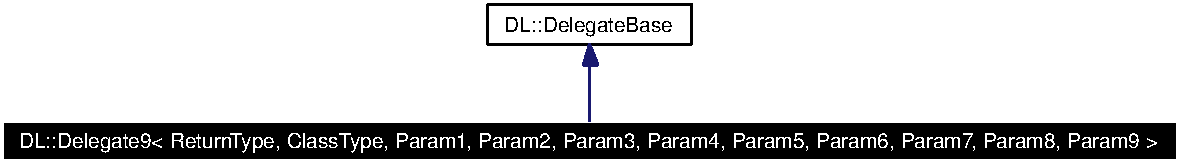
\includegraphics[width=300pt]{classDL_1_1Delegate9__inherit__graph}
\end{center}
\end{figure}
Collaboration diagram for DL::Delegate9$<$ Return\-Type, Class\-Type, Param1, Param2, Param3, Param4, Param5, Param6, Param7, Param8, Param9 $>$:\begin{figure}[H]
\begin{center}
\leavevmode
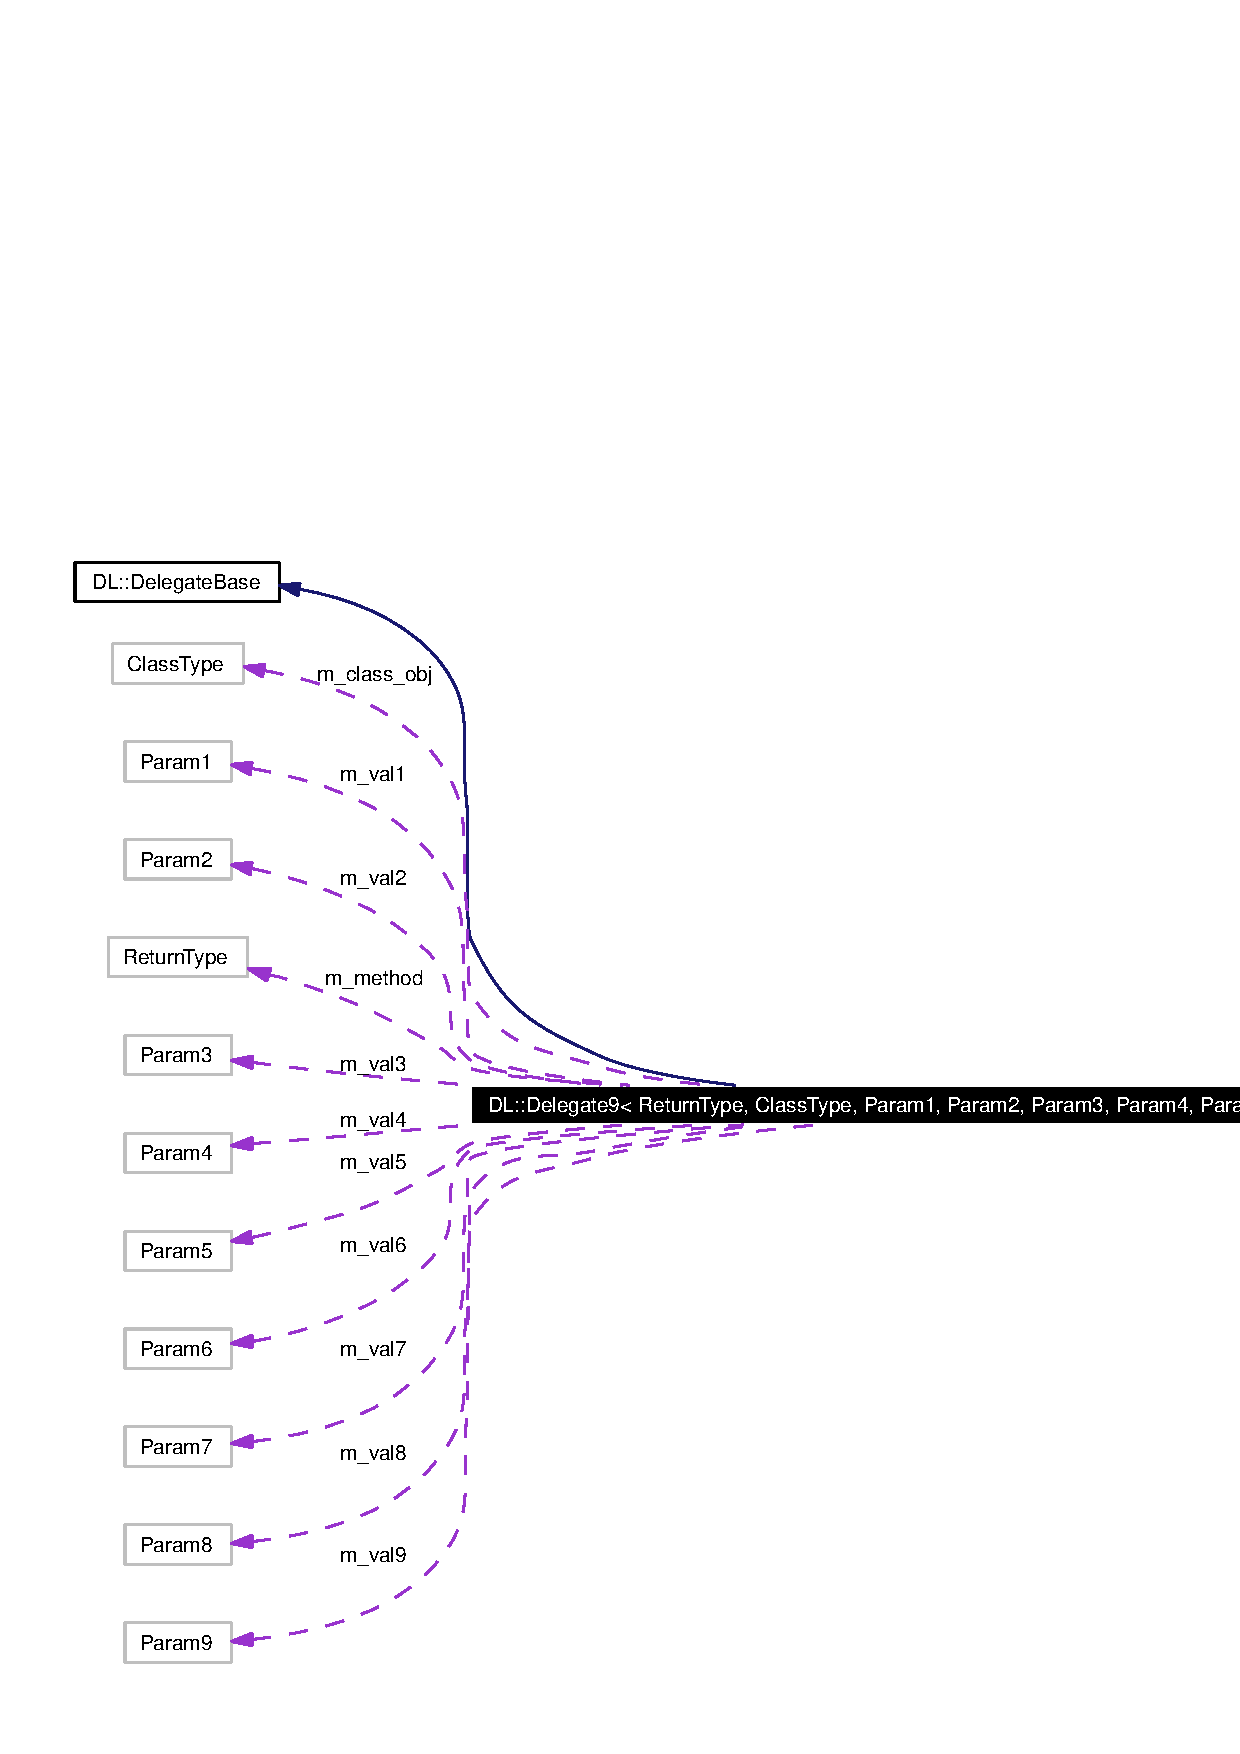
\includegraphics[width=395pt]{classDL_1_1Delegate9__coll__graph}
\end{center}
\end{figure}
\subsection*{Public Member Functions}
\begin{CompactItemize}
\item 
\hyperlink{classDL_1_1Delegate9_a0}{Delegate9} (Class\-Type $\ast$class\_\-obj, Return\-Type(Class\-Type::$\ast$method)(Param1, Param2, Param3, Param4, Param5, Param6, Param7, Param8, Param9), Param1 val1=Param1(), Param2 val2=Param2(), Param3 val3=Param3(), Param4 val4=Param4(), Param5 val5=Param5(), Param6 val6=Param6(), Param7 val7=Param7(), Param8 val8=Param8(), Param9 val9=Param9())
\item 
virtual \hyperlink{classDL_1_1Delegate9_a1}{$\sim$Delegate9} ()
\item 
void \hyperlink{classDL_1_1Delegate9_a2}{Invoke} ()
\item 
void \hyperlink{classDL_1_1Delegate9_a3}{Invoke} (Param1 val1, Param2 val2, Param3 val3, Param4 val4, Param5 val5, Param6 val6, Param7 val7, Param8 val8, Param9 val9)
\end{CompactItemize}
\subsection*{Private Member Functions}
\begin{CompactItemize}
\item 
\hyperlink{classDL_1_1Delegate9_d0}{Delegate9} ()
\end{CompactItemize}
\subsection*{Private Attributes}
\begin{CompactItemize}
\item 
Class\-Type $\ast$ \hyperlink{classDL_1_1Delegate9_r0}{m\_\-class\_\-obj}
\item 
Return\-Type(Class\-Type::$\ast$ \hyperlink{classDL_1_1Delegate9_r1}{m\_\-method} )(Param1, Param2, Param3, Param4, Param5, Param6, Param7, Param8, Param9)
\item 
Param1 \hyperlink{classDL_1_1Delegate9_r2}{m\_\-val1}
\item 
Param2 \hyperlink{classDL_1_1Delegate9_r3}{m\_\-val2}
\item 
Param3 \hyperlink{classDL_1_1Delegate9_r4}{m\_\-val3}
\item 
Param4 \hyperlink{classDL_1_1Delegate9_r5}{m\_\-val4}
\item 
Param5 \hyperlink{classDL_1_1Delegate9_r6}{m\_\-val5}
\item 
Param6 \hyperlink{classDL_1_1Delegate9_r7}{m\_\-val6}
\item 
Param7 \hyperlink{classDL_1_1Delegate9_r8}{m\_\-val7}
\item 
Param8 \hyperlink{classDL_1_1Delegate9_r9}{m\_\-val8}
\item 
Param9 \hyperlink{classDL_1_1Delegate9_r10}{m\_\-val9}
\end{CompactItemize}


\subsection{Detailed Description}
\subsubsection*{template$<$class Return\-Type, class Class\-Type, class Param1, class Param2, class Param3, class Param4, class Param5, class Param6, class Param7, class Param8, class Param9$>$ class DL::Delegate9$<$ Return\-Type, Class\-Type, Param1, Param2, Param3, Param4, Param5, Param6, Param7, Param8, Param9 $>$}

Delegate for 9 Param



Definition at line 40 of file Delegate9.hpp.

\subsection{Constructor \& Destructor Documentation}
\hypertarget{classDL_1_1Delegate9_d0}{
\index{DL::Delegate9@{DL::Delegate9}!Delegate9@{Delegate9}}
\index{Delegate9@{Delegate9}!DL::Delegate9@{DL::Delegate9}}
\subsubsection[Delegate9]{\setlength{\rightskip}{0pt plus 5cm}template$<$class Return\-Type, class Class\-Type, class Param1, class Param2, class Param3, class Param4, class Param5, class Param6, class Param7, class Param8, class Param9$>$ \hyperlink{classDL_1_1Delegate9}{DL::Delegate9}$<$ Return\-Type, Class\-Type, Param1, Param2, Param3, Param4, Param5, Param6, Param7, Param8, Param9 $>$::\hyperlink{classDL_1_1Delegate9}{Delegate9} ()\hspace{0.3cm}{\tt  \mbox{[}inline, private\mbox{]}}}}
\label{classDL_1_1Delegate9_d0}




Definition at line 53 of file Delegate9.hpp.\hypertarget{classDL_1_1Delegate9_a0}{
\index{DL::Delegate9@{DL::Delegate9}!Delegate9@{Delegate9}}
\index{Delegate9@{Delegate9}!DL::Delegate9@{DL::Delegate9}}
\subsubsection[Delegate9]{\setlength{\rightskip}{0pt plus 5cm}template$<$class Return\-Type, class Class\-Type, class Param1, class Param2, class Param3, class Param4, class Param5, class Param6, class Param7, class Param8, class Param9$>$ \hyperlink{classDL_1_1Delegate9}{DL::Delegate9}$<$ Return\-Type, Class\-Type, Param1, Param2, Param3, Param4, Param5, Param6, Param7, Param8, Param9 $>$::\hyperlink{classDL_1_1Delegate9}{Delegate9} (Class\-Type $\ast$ {\em class\_\-obj}, Return\-Type(Class\-Type::$\ast$)(Param1, Param2, Param3, Param4, Param5, Param6, Param7, Param8, Param9) {\em method}, Param1 {\em val1} = {\tt Param1()}, Param2 {\em val2} = {\tt Param2()}, Param3 {\em val3} = {\tt Param3()}, Param4 {\em val4} = {\tt Param4()}, Param5 {\em val5} = {\tt Param5()}, Param6 {\em val6} = {\tt Param6()}, Param7 {\em val7} = {\tt Param7()}, Param8 {\em val8} = {\tt Param8()}, Param9 {\em val9} = {\tt Param9()})\hspace{0.3cm}{\tt  \mbox{[}inline\mbox{]}}}}
\label{classDL_1_1Delegate9_a0}




Definition at line 55 of file Delegate9.hpp.

References DL::Delegate9$<$ Return\-Type, Class\-Type, Param1, Param2, Param3, Param4, Param5, Param6, Param7, Param8, Param9 $>$::m\_\-class\_\-obj, DL::Delegate9$<$ Return\-Type, Class\-Type, Param1, Param2, Param3, Param4, Param5, Param6, Param7, Param8, Param9 $>$::m\_\-method, DL::Delegate9$<$ Return\-Type, Class\-Type, Param1, Param2, Param3, Param4, Param5, Param6, Param7, Param8, Param9 $>$::m\_\-val1, DL::Delegate9$<$ Return\-Type, Class\-Type, Param1, Param2, Param3, Param4, Param5, Param6, Param7, Param8, Param9 $>$::m\_\-val2, DL::Delegate9$<$ Return\-Type, Class\-Type, Param1, Param2, Param3, Param4, Param5, Param6, Param7, Param8, Param9 $>$::m\_\-val3, DL::Delegate9$<$ Return\-Type, Class\-Type, Param1, Param2, Param3, Param4, Param5, Param6, Param7, Param8, Param9 $>$::m\_\-val4, DL::Delegate9$<$ Return\-Type, Class\-Type, Param1, Param2, Param3, Param4, Param5, Param6, Param7, Param8, Param9 $>$::m\_\-val5, DL::Delegate9$<$ Return\-Type, Class\-Type, Param1, Param2, Param3, Param4, Param5, Param6, Param7, Param8, Param9 $>$::m\_\-val6, DL::Delegate9$<$ Return\-Type, Class\-Type, Param1, Param2, Param3, Param4, Param5, Param6, Param7, Param8, Param9 $>$::m\_\-val7, DL::Delegate9$<$ Return\-Type, Class\-Type, Param1, Param2, Param3, Param4, Param5, Param6, Param7, Param8, Param9 $>$::m\_\-val8, and DL::Delegate9$<$ Return\-Type, Class\-Type, Param1, Param2, Param3, Param4, Param5, Param6, Param7, Param8, Param9 $>$::m\_\-val9.\hypertarget{classDL_1_1Delegate9_a1}{
\index{DL::Delegate9@{DL::Delegate9}!~Delegate9@{$\sim$Delegate9}}
\index{~Delegate9@{$\sim$Delegate9}!DL::Delegate9@{DL::Delegate9}}
\subsubsection[$\sim$Delegate9]{\setlength{\rightskip}{0pt plus 5cm}template$<$class Return\-Type, class Class\-Type, class Param1, class Param2, class Param3, class Param4, class Param5, class Param6, class Param7, class Param8, class Param9$>$ virtual \hyperlink{classDL_1_1Delegate9}{DL::Delegate9}$<$ Return\-Type, Class\-Type, Param1, Param2, Param3, Param4, Param5, Param6, Param7, Param8, Param9 $>$::$\sim$\hyperlink{classDL_1_1Delegate9}{Delegate9} ()\hspace{0.3cm}{\tt  \mbox{[}inline, virtual\mbox{]}}}}
\label{classDL_1_1Delegate9_a1}




Definition at line 71 of file Delegate9.hpp.

\subsection{Member Function Documentation}
\hypertarget{classDL_1_1Delegate9_a3}{
\index{DL::Delegate9@{DL::Delegate9}!Invoke@{Invoke}}
\index{Invoke@{Invoke}!DL::Delegate9@{DL::Delegate9}}
\subsubsection[Invoke]{\setlength{\rightskip}{0pt plus 5cm}template$<$class Return\-Type, class Class\-Type, class Param1, class Param2, class Param3, class Param4, class Param5, class Param6, class Param7, class Param8, class Param9$>$ void \hyperlink{classDL_1_1Delegate9}{DL::Delegate9}$<$ Return\-Type, Class\-Type, Param1, Param2, Param3, Param4, Param5, Param6, Param7, Param8, Param9 $>$::Invoke (Param1 {\em val1}, Param2 {\em val2}, Param3 {\em val3}, Param4 {\em val4}, Param5 {\em val5}, Param6 {\em val6}, Param7 {\em val7}, Param8 {\em val8}, Param9 {\em val9})\hspace{0.3cm}{\tt  \mbox{[}inline\mbox{]}}}}
\label{classDL_1_1Delegate9_a3}




Definition at line 76 of file Delegate9.hpp.

References DL::Delegate9$<$ Return\-Type, Class\-Type, Param1, Param2, Param3, Param4, Param5, Param6, Param7, Param8, Param9 $>$::m\_\-class\_\-obj, and DL::Delegate9$<$ Return\-Type, Class\-Type, Param1, Param2, Param3, Param4, Param5, Param6, Param7, Param8, Param9 $>$::m\_\-method.\hypertarget{classDL_1_1Delegate9_a2}{
\index{DL::Delegate9@{DL::Delegate9}!Invoke@{Invoke}}
\index{Invoke@{Invoke}!DL::Delegate9@{DL::Delegate9}}
\subsubsection[Invoke]{\setlength{\rightskip}{0pt plus 5cm}template$<$class Return\-Type, class Class\-Type, class Param1, class Param2, class Param3, class Param4, class Param5, class Param6, class Param7, class Param8, class Param9$>$ void \hyperlink{classDL_1_1Delegate9}{DL::Delegate9}$<$ Return\-Type, Class\-Type, Param1, Param2, Param3, Param4, Param5, Param6, Param7, Param8, Param9 $>$::Invoke ()\hspace{0.3cm}{\tt  \mbox{[}inline, virtual\mbox{]}}}}
\label{classDL_1_1Delegate9_a2}




Implements \hyperlink{classDL_1_1DelegateBase_a2}{DL::Delegate\-Base}.

Definition at line 72 of file Delegate9.hpp.

References DL::Delegate9$<$ Return\-Type, Class\-Type, Param1, Param2, Param3, Param4, Param5, Param6, Param7, Param8, Param9 $>$::m\_\-class\_\-obj, DL::Delegate9$<$ Return\-Type, Class\-Type, Param1, Param2, Param3, Param4, Param5, Param6, Param7, Param8, Param9 $>$::m\_\-method, DL::Delegate9$<$ Return\-Type, Class\-Type, Param1, Param2, Param3, Param4, Param5, Param6, Param7, Param8, Param9 $>$::m\_\-val1, DL::Delegate9$<$ Return\-Type, Class\-Type, Param1, Param2, Param3, Param4, Param5, Param6, Param7, Param8, Param9 $>$::m\_\-val2, DL::Delegate9$<$ Return\-Type, Class\-Type, Param1, Param2, Param3, Param4, Param5, Param6, Param7, Param8, Param9 $>$::m\_\-val3, DL::Delegate9$<$ Return\-Type, Class\-Type, Param1, Param2, Param3, Param4, Param5, Param6, Param7, Param8, Param9 $>$::m\_\-val4, DL::Delegate9$<$ Return\-Type, Class\-Type, Param1, Param2, Param3, Param4, Param5, Param6, Param7, Param8, Param9 $>$::m\_\-val5, DL::Delegate9$<$ Return\-Type, Class\-Type, Param1, Param2, Param3, Param4, Param5, Param6, Param7, Param8, Param9 $>$::m\_\-val6, DL::Delegate9$<$ Return\-Type, Class\-Type, Param1, Param2, Param3, Param4, Param5, Param6, Param7, Param8, Param9 $>$::m\_\-val7, DL::Delegate9$<$ Return\-Type, Class\-Type, Param1, Param2, Param3, Param4, Param5, Param6, Param7, Param8, Param9 $>$::m\_\-val8, and DL::Delegate9$<$ Return\-Type, Class\-Type, Param1, Param2, Param3, Param4, Param5, Param6, Param7, Param8, Param9 $>$::m\_\-val9.

\subsection{Member Data Documentation}
\hypertarget{classDL_1_1Delegate9_r0}{
\index{DL::Delegate9@{DL::Delegate9}!m_class_obj@{m\_\-class\_\-obj}}
\index{m_class_obj@{m\_\-class\_\-obj}!DL::Delegate9@{DL::Delegate9}}
\subsubsection[m\_\-class\_\-obj]{\setlength{\rightskip}{0pt plus 5cm}template$<$class Return\-Type, class Class\-Type, class Param1, class Param2, class Param3, class Param4, class Param5, class Param6, class Param7, class Param8, class Param9$>$ Class\-Type$\ast$ \hyperlink{classDL_1_1Delegate9}{DL::Delegate9}$<$ Return\-Type, Class\-Type, Param1, Param2, Param3, Param4, Param5, Param6, Param7, Param8, Param9 $>$::\hyperlink{classDL_1_1Delegate9_r0}{m\_\-class\_\-obj}\hspace{0.3cm}{\tt  \mbox{[}private\mbox{]}}}}
\label{classDL_1_1Delegate9_r0}




Definition at line 42 of file Delegate9.hpp.

Referenced by DL::Delegate9$<$ Return\-Type, Class\-Type, Param1, Param2, Param3, Param4, Param5, Param6, Param7, Param8, Param9 $>$::Delegate9(), and DL::Delegate9$<$ Return\-Type, Class\-Type, Param1, Param2, Param3, Param4, Param5, Param6, Param7, Param8, Param9 $>$::Invoke().\hypertarget{classDL_1_1Delegate9_r1}{
\index{DL::Delegate9@{DL::Delegate9}!m_method@{m\_\-method}}
\index{m_method@{m\_\-method}!DL::Delegate9@{DL::Delegate9}}
\subsubsection[m\_\-method]{\setlength{\rightskip}{0pt plus 5cm}template$<$class Return\-Type, class Class\-Type, class Param1, class Param2, class Param3, class Param4, class Param5, class Param6, class Param7, class Param8, class Param9$>$ Return\-Type(Class\-Type::$\ast$ \hyperlink{classDL_1_1Delegate9}{DL::Delegate9}$<$ Return\-Type, Class\-Type, Param1, Param2, Param3, Param4, Param5, Param6, Param7, Param8, Param9 $>$::\hyperlink{classDL_1_1Delegate9_r1}{m\_\-method})(Param1, Param2, Param3, Param4, Param5, Param6, Param7, Param8, Param9)\hspace{0.3cm}{\tt  \mbox{[}private\mbox{]}}}}
\label{classDL_1_1Delegate9_r1}




Referenced by DL::Delegate9$<$ Return\-Type, Class\-Type, Param1, Param2, Param3, Param4, Param5, Param6, Param7, Param8, Param9 $>$::Delegate9(), and DL::Delegate9$<$ Return\-Type, Class\-Type, Param1, Param2, Param3, Param4, Param5, Param6, Param7, Param8, Param9 $>$::Invoke().\hypertarget{classDL_1_1Delegate9_r2}{
\index{DL::Delegate9@{DL::Delegate9}!m_val1@{m\_\-val1}}
\index{m_val1@{m\_\-val1}!DL::Delegate9@{DL::Delegate9}}
\subsubsection[m\_\-val1]{\setlength{\rightskip}{0pt plus 5cm}template$<$class Return\-Type, class Class\-Type, class Param1, class Param2, class Param3, class Param4, class Param5, class Param6, class Param7, class Param8, class Param9$>$ Param1 \hyperlink{classDL_1_1Delegate9}{DL::Delegate9}$<$ Return\-Type, Class\-Type, Param1, Param2, Param3, Param4, Param5, Param6, Param7, Param8, Param9 $>$::\hyperlink{classDL_1_1Delegate9_r2}{m\_\-val1}\hspace{0.3cm}{\tt  \mbox{[}private\mbox{]}}}}
\label{classDL_1_1Delegate9_r2}




Definition at line 44 of file Delegate9.hpp.

Referenced by DL::Delegate9$<$ Return\-Type, Class\-Type, Param1, Param2, Param3, Param4, Param5, Param6, Param7, Param8, Param9 $>$::Delegate9(), and DL::Delegate9$<$ Return\-Type, Class\-Type, Param1, Param2, Param3, Param4, Param5, Param6, Param7, Param8, Param9 $>$::Invoke().\hypertarget{classDL_1_1Delegate9_r3}{
\index{DL::Delegate9@{DL::Delegate9}!m_val2@{m\_\-val2}}
\index{m_val2@{m\_\-val2}!DL::Delegate9@{DL::Delegate9}}
\subsubsection[m\_\-val2]{\setlength{\rightskip}{0pt plus 5cm}template$<$class Return\-Type, class Class\-Type, class Param1, class Param2, class Param3, class Param4, class Param5, class Param6, class Param7, class Param8, class Param9$>$ Param2 \hyperlink{classDL_1_1Delegate9}{DL::Delegate9}$<$ Return\-Type, Class\-Type, Param1, Param2, Param3, Param4, Param5, Param6, Param7, Param8, Param9 $>$::\hyperlink{classDL_1_1Delegate9_r3}{m\_\-val2}\hspace{0.3cm}{\tt  \mbox{[}private\mbox{]}}}}
\label{classDL_1_1Delegate9_r3}




Definition at line 45 of file Delegate9.hpp.

Referenced by DL::Delegate9$<$ Return\-Type, Class\-Type, Param1, Param2, Param3, Param4, Param5, Param6, Param7, Param8, Param9 $>$::Delegate9(), and DL::Delegate9$<$ Return\-Type, Class\-Type, Param1, Param2, Param3, Param4, Param5, Param6, Param7, Param8, Param9 $>$::Invoke().\hypertarget{classDL_1_1Delegate9_r4}{
\index{DL::Delegate9@{DL::Delegate9}!m_val3@{m\_\-val3}}
\index{m_val3@{m\_\-val3}!DL::Delegate9@{DL::Delegate9}}
\subsubsection[m\_\-val3]{\setlength{\rightskip}{0pt plus 5cm}template$<$class Return\-Type, class Class\-Type, class Param1, class Param2, class Param3, class Param4, class Param5, class Param6, class Param7, class Param8, class Param9$>$ Param3 \hyperlink{classDL_1_1Delegate9}{DL::Delegate9}$<$ Return\-Type, Class\-Type, Param1, Param2, Param3, Param4, Param5, Param6, Param7, Param8, Param9 $>$::\hyperlink{classDL_1_1Delegate9_r4}{m\_\-val3}\hspace{0.3cm}{\tt  \mbox{[}private\mbox{]}}}}
\label{classDL_1_1Delegate9_r4}




Definition at line 46 of file Delegate9.hpp.

Referenced by DL::Delegate9$<$ Return\-Type, Class\-Type, Param1, Param2, Param3, Param4, Param5, Param6, Param7, Param8, Param9 $>$::Delegate9(), and DL::Delegate9$<$ Return\-Type, Class\-Type, Param1, Param2, Param3, Param4, Param5, Param6, Param7, Param8, Param9 $>$::Invoke().\hypertarget{classDL_1_1Delegate9_r5}{
\index{DL::Delegate9@{DL::Delegate9}!m_val4@{m\_\-val4}}
\index{m_val4@{m\_\-val4}!DL::Delegate9@{DL::Delegate9}}
\subsubsection[m\_\-val4]{\setlength{\rightskip}{0pt plus 5cm}template$<$class Return\-Type, class Class\-Type, class Param1, class Param2, class Param3, class Param4, class Param5, class Param6, class Param7, class Param8, class Param9$>$ Param4 \hyperlink{classDL_1_1Delegate9}{DL::Delegate9}$<$ Return\-Type, Class\-Type, Param1, Param2, Param3, Param4, Param5, Param6, Param7, Param8, Param9 $>$::\hyperlink{classDL_1_1Delegate9_r5}{m\_\-val4}\hspace{0.3cm}{\tt  \mbox{[}private\mbox{]}}}}
\label{classDL_1_1Delegate9_r5}




Definition at line 47 of file Delegate9.hpp.

Referenced by DL::Delegate9$<$ Return\-Type, Class\-Type, Param1, Param2, Param3, Param4, Param5, Param6, Param7, Param8, Param9 $>$::Delegate9(), and DL::Delegate9$<$ Return\-Type, Class\-Type, Param1, Param2, Param3, Param4, Param5, Param6, Param7, Param8, Param9 $>$::Invoke().\hypertarget{classDL_1_1Delegate9_r6}{
\index{DL::Delegate9@{DL::Delegate9}!m_val5@{m\_\-val5}}
\index{m_val5@{m\_\-val5}!DL::Delegate9@{DL::Delegate9}}
\subsubsection[m\_\-val5]{\setlength{\rightskip}{0pt plus 5cm}template$<$class Return\-Type, class Class\-Type, class Param1, class Param2, class Param3, class Param4, class Param5, class Param6, class Param7, class Param8, class Param9$>$ Param5 \hyperlink{classDL_1_1Delegate9}{DL::Delegate9}$<$ Return\-Type, Class\-Type, Param1, Param2, Param3, Param4, Param5, Param6, Param7, Param8, Param9 $>$::\hyperlink{classDL_1_1Delegate9_r6}{m\_\-val5}\hspace{0.3cm}{\tt  \mbox{[}private\mbox{]}}}}
\label{classDL_1_1Delegate9_r6}




Definition at line 48 of file Delegate9.hpp.

Referenced by DL::Delegate9$<$ Return\-Type, Class\-Type, Param1, Param2, Param3, Param4, Param5, Param6, Param7, Param8, Param9 $>$::Delegate9(), and DL::Delegate9$<$ Return\-Type, Class\-Type, Param1, Param2, Param3, Param4, Param5, Param6, Param7, Param8, Param9 $>$::Invoke().\hypertarget{classDL_1_1Delegate9_r7}{
\index{DL::Delegate9@{DL::Delegate9}!m_val6@{m\_\-val6}}
\index{m_val6@{m\_\-val6}!DL::Delegate9@{DL::Delegate9}}
\subsubsection[m\_\-val6]{\setlength{\rightskip}{0pt plus 5cm}template$<$class Return\-Type, class Class\-Type, class Param1, class Param2, class Param3, class Param4, class Param5, class Param6, class Param7, class Param8, class Param9$>$ Param6 \hyperlink{classDL_1_1Delegate9}{DL::Delegate9}$<$ Return\-Type, Class\-Type, Param1, Param2, Param3, Param4, Param5, Param6, Param7, Param8, Param9 $>$::\hyperlink{classDL_1_1Delegate9_r7}{m\_\-val6}\hspace{0.3cm}{\tt  \mbox{[}private\mbox{]}}}}
\label{classDL_1_1Delegate9_r7}




Definition at line 49 of file Delegate9.hpp.

Referenced by DL::Delegate9$<$ Return\-Type, Class\-Type, Param1, Param2, Param3, Param4, Param5, Param6, Param7, Param8, Param9 $>$::Delegate9(), and DL::Delegate9$<$ Return\-Type, Class\-Type, Param1, Param2, Param3, Param4, Param5, Param6, Param7, Param8, Param9 $>$::Invoke().\hypertarget{classDL_1_1Delegate9_r8}{
\index{DL::Delegate9@{DL::Delegate9}!m_val7@{m\_\-val7}}
\index{m_val7@{m\_\-val7}!DL::Delegate9@{DL::Delegate9}}
\subsubsection[m\_\-val7]{\setlength{\rightskip}{0pt plus 5cm}template$<$class Return\-Type, class Class\-Type, class Param1, class Param2, class Param3, class Param4, class Param5, class Param6, class Param7, class Param8, class Param9$>$ Param7 \hyperlink{classDL_1_1Delegate9}{DL::Delegate9}$<$ Return\-Type, Class\-Type, Param1, Param2, Param3, Param4, Param5, Param6, Param7, Param8, Param9 $>$::\hyperlink{classDL_1_1Delegate9_r8}{m\_\-val7}\hspace{0.3cm}{\tt  \mbox{[}private\mbox{]}}}}
\label{classDL_1_1Delegate9_r8}




Definition at line 50 of file Delegate9.hpp.

Referenced by DL::Delegate9$<$ Return\-Type, Class\-Type, Param1, Param2, Param3, Param4, Param5, Param6, Param7, Param8, Param9 $>$::Delegate9(), and DL::Delegate9$<$ Return\-Type, Class\-Type, Param1, Param2, Param3, Param4, Param5, Param6, Param7, Param8, Param9 $>$::Invoke().\hypertarget{classDL_1_1Delegate9_r9}{
\index{DL::Delegate9@{DL::Delegate9}!m_val8@{m\_\-val8}}
\index{m_val8@{m\_\-val8}!DL::Delegate9@{DL::Delegate9}}
\subsubsection[m\_\-val8]{\setlength{\rightskip}{0pt plus 5cm}template$<$class Return\-Type, class Class\-Type, class Param1, class Param2, class Param3, class Param4, class Param5, class Param6, class Param7, class Param8, class Param9$>$ Param8 \hyperlink{classDL_1_1Delegate9}{DL::Delegate9}$<$ Return\-Type, Class\-Type, Param1, Param2, Param3, Param4, Param5, Param6, Param7, Param8, Param9 $>$::\hyperlink{classDL_1_1Delegate9_r9}{m\_\-val8}\hspace{0.3cm}{\tt  \mbox{[}private\mbox{]}}}}
\label{classDL_1_1Delegate9_r9}




Definition at line 51 of file Delegate9.hpp.

Referenced by DL::Delegate9$<$ Return\-Type, Class\-Type, Param1, Param2, Param3, Param4, Param5, Param6, Param7, Param8, Param9 $>$::Delegate9(), and DL::Delegate9$<$ Return\-Type, Class\-Type, Param1, Param2, Param3, Param4, Param5, Param6, Param7, Param8, Param9 $>$::Invoke().\hypertarget{classDL_1_1Delegate9_r10}{
\index{DL::Delegate9@{DL::Delegate9}!m_val9@{m\_\-val9}}
\index{m_val9@{m\_\-val9}!DL::Delegate9@{DL::Delegate9}}
\subsubsection[m\_\-val9]{\setlength{\rightskip}{0pt plus 5cm}template$<$class Return\-Type, class Class\-Type, class Param1, class Param2, class Param3, class Param4, class Param5, class Param6, class Param7, class Param8, class Param9$>$ Param9 \hyperlink{classDL_1_1Delegate9}{DL::Delegate9}$<$ Return\-Type, Class\-Type, Param1, Param2, Param3, Param4, Param5, Param6, Param7, Param8, Param9 $>$::\hyperlink{classDL_1_1Delegate9_r10}{m\_\-val9}\hspace{0.3cm}{\tt  \mbox{[}private\mbox{]}}}}
\label{classDL_1_1Delegate9_r10}




Definition at line 52 of file Delegate9.hpp.

Referenced by DL::Delegate9$<$ Return\-Type, Class\-Type, Param1, Param2, Param3, Param4, Param5, Param6, Param7, Param8, Param9 $>$::Delegate9(), and DL::Delegate9$<$ Return\-Type, Class\-Type, Param1, Param2, Param3, Param4, Param5, Param6, Param7, Param8, Param9 $>$::Invoke().

The documentation for this class was generated from the following file:\begin{CompactItemize}
\item 
/data/callbackext/Delegate\-N/\hyperlink{Delegate9_8hpp}{Delegate9.hpp}\end{CompactItemize}

\hypertarget{classDL_1_1DelegateBase}{
\section{DL::Delegate\-Base Class Reference}
\label{classDL_1_1DelegateBase}\index{DL::DelegateBase@{DL::DelegateBase}}
}
{\tt \#include $<$Delegate\-Base.hpp$>$}

Inherited by \hyperlink{classDL_1_1Delegate0}{DL::Delegate0$<$ Return\-Type, Class\-Type $>$}, \hyperlink{classDL_1_1Delegate1}{DL::Delegate1$<$ Return\-Type, Class\-Type, Param1 $>$}, \hyperlink{classDL_1_1Delegate10}{DL::Delegate10$<$ Return\-Type, Class\-Type, Param1, Param2, Param3, Param4, Param5, Param6, Param7, Param8, Param9, Param10 $>$}, \hyperlink{classDL_1_1Delegate2}{DL::Delegate2$<$ Return\-Type, Class\-Type, Param1, Param2 $>$}, \hyperlink{classDL_1_1Delegate3}{DL::Delegate3$<$ Return\-Type, Class\-Type, Param1, Param2, Param3 $>$}, \hyperlink{classDL_1_1Delegate4}{DL::Delegate4$<$ Return\-Type, Class\-Type, Param1, Param2, Param3, Param4 $>$}, \hyperlink{classDL_1_1Delegate5}{DL::Delegate5$<$ Return\-Type, Class\-Type, Param1, Param2, Param3, Param4, Param5 $>$}, \hyperlink{classDL_1_1Delegate6}{DL::Delegate6$<$ Return\-Type, Class\-Type, Param1, Param2, Param3, Param4, Param5, Param6 $>$}, \hyperlink{classDL_1_1Delegate7}{DL::Delegate7$<$ Return\-Type, Class\-Type, Param1, Param2, Param3, Param4, Param5, Param6, Param7 $>$}, \hyperlink{classDL_1_1Delegate8}{DL::Delegate8$<$ Return\-Type, Class\-Type, Param1, Param2, Param3, Param4, Param5, Param6, Param7, Param8 $>$}, \hyperlink{classDL_1_1Delegate9}{DL::Delegate9$<$ Return\-Type, Class\-Type, Param1, Param2, Param3, Param4, Param5, Param6, Param7, Param8, Param9 $>$}, \hyperlink{classDL_1_1Functor0}{DL::Functor0}, \hyperlink{classDL_1_1Functor1}{DL::Functor1$<$ Return\-Type, Param1 $>$}, \hyperlink{classDL_1_1Functor10}{DL::Functor10$<$ Return\-Type, Param1, Param2, Param3, Param4, Param5, Param6, Param7, Param8, Param9, Param10 $>$}, \hyperlink{classDL_1_1Functor2}{DL::Functor2$<$ Return\-Type, Param1, Param2 $>$}, \hyperlink{classDL_1_1Functor3}{DL::Functor3$<$ Return\-Type, Param1, Param2, Param3 $>$}, \hyperlink{classDL_1_1Functor4}{DL::Functor4$<$ Return\-Type, Param1, Param2, Param3, Param4 $>$}, \hyperlink{classDL_1_1Functor5}{DL::Functor5$<$ Return\-Type, Param1, Param2, Param3, Param4, Param5 $>$}, \hyperlink{classDL_1_1Functor6}{DL::Functor6$<$ Return\-Type, Param1, Param2, Param3, Param4, Param5, Param6 $>$}, \hyperlink{classDL_1_1Functor7}{DL::Functor7$<$ Return\-Type, Param1, Param2, Param3, Param4, Param5, Param6, Param7 $>$}, \hyperlink{classDL_1_1Functor8}{DL::Functor8$<$ Return\-Type, Param1, Param2, Param3, Param4, Param5, Param6, Param7, Param8 $>$}, and \hyperlink{classDL_1_1Functor9}{DL::Functor9$<$ Return\-Type, Param1, Param2, Param3, Param4, Param5, Param6, Param7, Param8, Param9 $>$}.

Inheritance diagram for DL::Delegate\-Base:\begin{figure}[H]
\begin{center}
\leavevmode
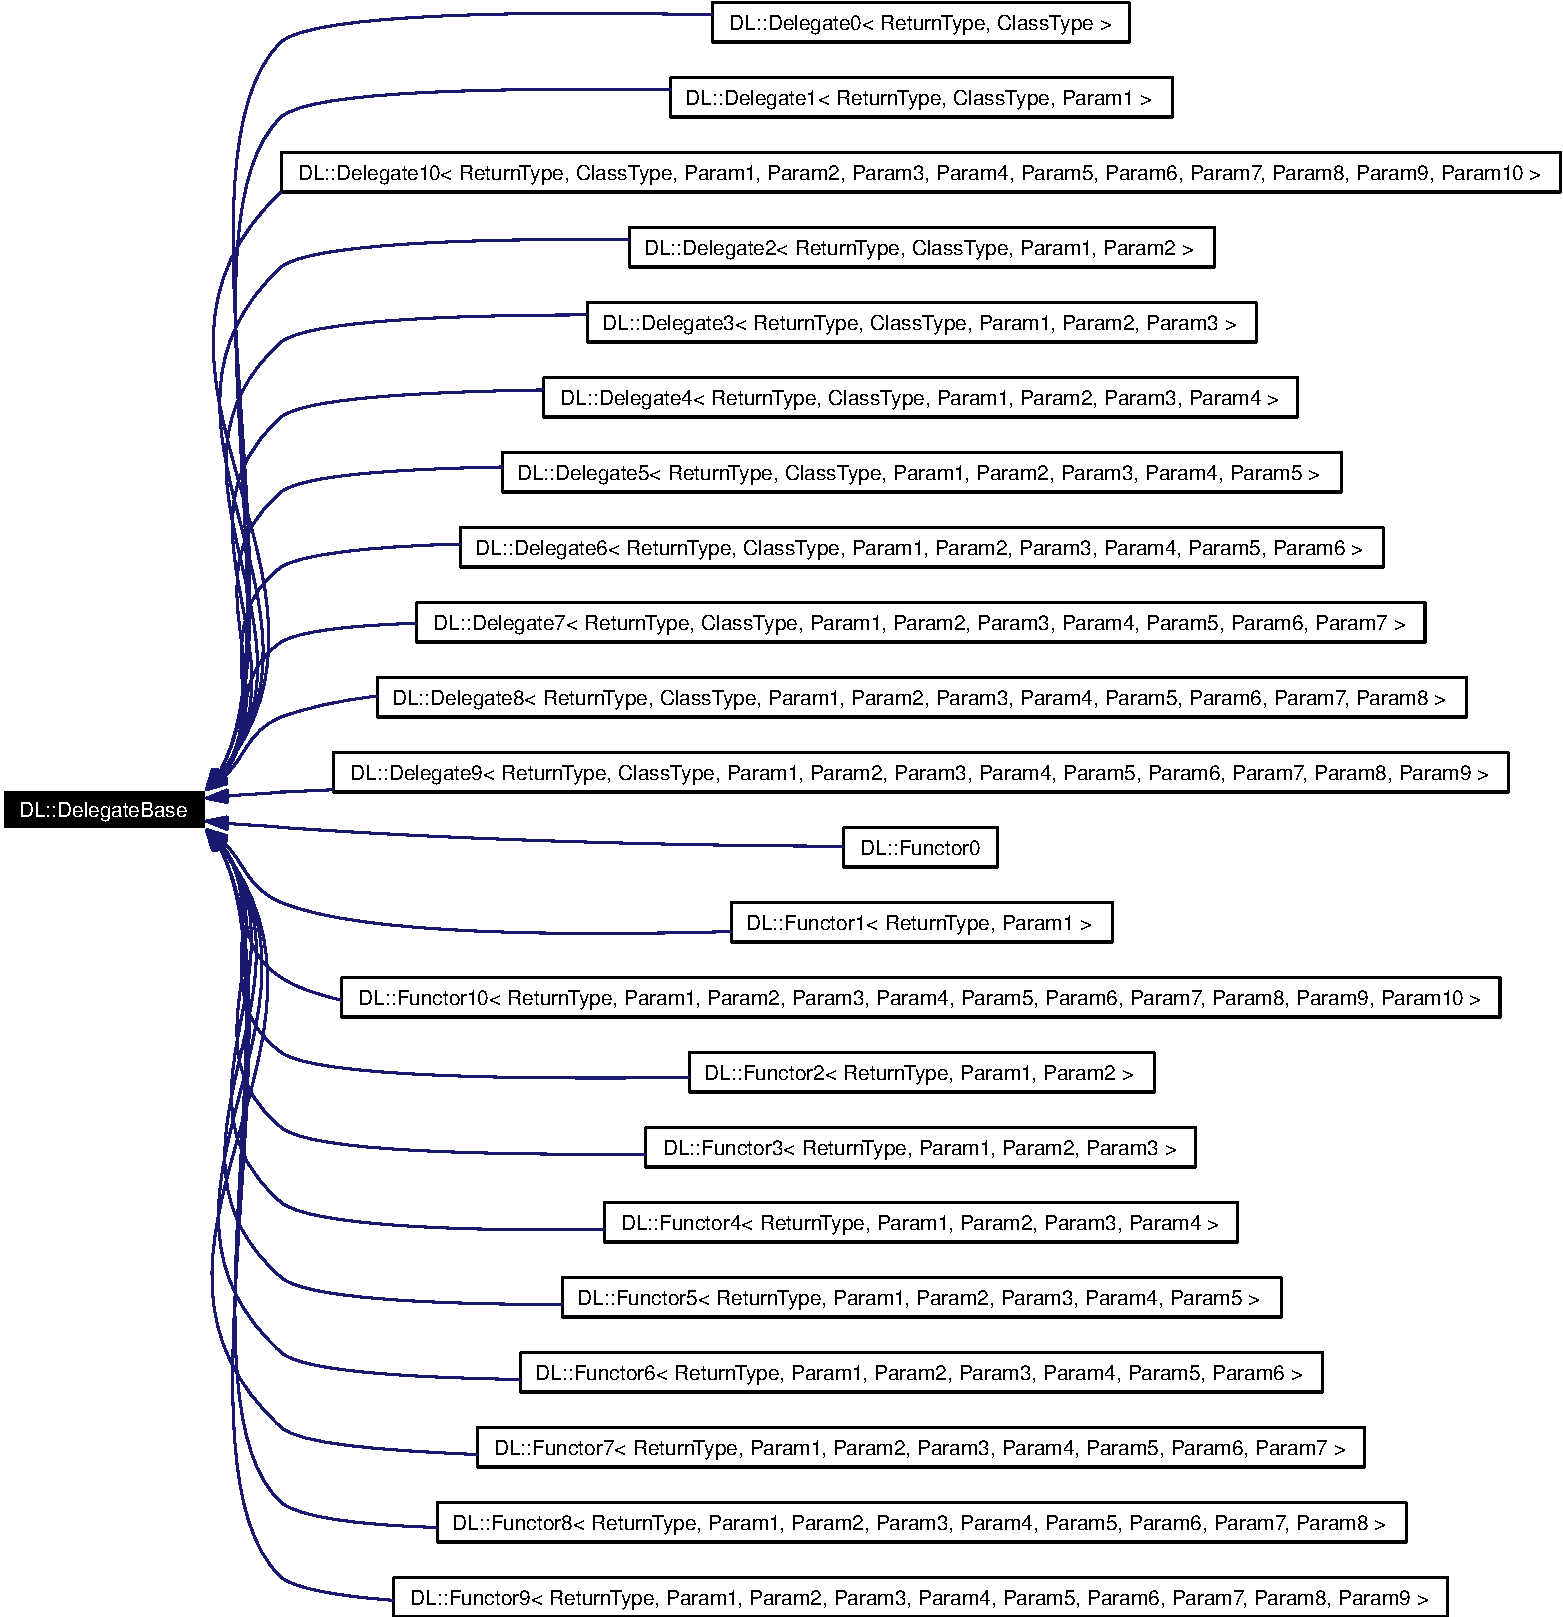
\includegraphics[width=392pt]{classDL_1_1DelegateBase__inherit__graph}
\end{center}
\end{figure}
\subsection*{Public Member Functions}
\begin{CompactItemize}
\item 
\hyperlink{classDL_1_1DelegateBase_a0}{Delegate\-Base} ()
\item 
virtual \hyperlink{classDL_1_1DelegateBase_a1}{$\sim$Delegate\-Base} ()
\item 
virtual void \hyperlink{classDL_1_1DelegateBase_a2}{Invoke} ()=0
\end{CompactItemize}


\subsection{Constructor \& Destructor Documentation}
\hypertarget{classDL_1_1DelegateBase_a0}{
\index{DL::DelegateBase@{DL::Delegate\-Base}!DelegateBase@{DelegateBase}}
\index{DelegateBase@{DelegateBase}!DL::DelegateBase@{DL::Delegate\-Base}}
\subsubsection[DelegateBase]{\setlength{\rightskip}{0pt plus 5cm}DL::Delegate\-Base::Delegate\-Base ()\hspace{0.3cm}{\tt  \mbox{[}inline\mbox{]}}}}
\label{classDL_1_1DelegateBase_a0}




Definition at line 28 of file Delegate\-Base.hpp.\hypertarget{classDL_1_1DelegateBase_a1}{
\index{DL::DelegateBase@{DL::Delegate\-Base}!~DelegateBase@{$\sim$DelegateBase}}
\index{~DelegateBase@{$\sim$DelegateBase}!DL::DelegateBase@{DL::Delegate\-Base}}
\subsubsection[$\sim$DelegateBase]{\setlength{\rightskip}{0pt plus 5cm}virtual DL::Delegate\-Base::$\sim$\hyperlink{classDL_1_1DelegateBase}{Delegate\-Base} ()\hspace{0.3cm}{\tt  \mbox{[}inline, virtual\mbox{]}}}}
\label{classDL_1_1DelegateBase_a1}




Definition at line 29 of file Delegate\-Base.hpp.

\subsection{Member Function Documentation}
\hypertarget{classDL_1_1DelegateBase_a2}{
\index{DL::DelegateBase@{DL::Delegate\-Base}!Invoke@{Invoke}}
\index{Invoke@{Invoke}!DL::DelegateBase@{DL::Delegate\-Base}}
\subsubsection[Invoke]{\setlength{\rightskip}{0pt plus 5cm}virtual void DL::Delegate\-Base::Invoke ()\hspace{0.3cm}{\tt  \mbox{[}pure virtual\mbox{]}}}}
\label{classDL_1_1DelegateBase_a2}




Implemented in \hyperlink{classDL_1_1Delegate0_a2}{DL::Delegate0$<$ Return\-Type, Class\-Type $>$}, \hyperlink{classDL_1_1Delegate1_a2}{DL::Delegate1$<$ Return\-Type, Class\-Type, Param1 $>$}, \hyperlink{classDL_1_1Delegate10_a2}{DL::Delegate10$<$ Return\-Type, Class\-Type, Param1, Param2, Param3, Param4, Param5, Param6, Param7, Param8, Param9, Param10 $>$}, \hyperlink{classDL_1_1Delegate2_a2}{DL::Delegate2$<$ Return\-Type, Class\-Type, Param1, Param2 $>$}, \hyperlink{classDL_1_1Delegate3_a2}{DL::Delegate3$<$ Return\-Type, Class\-Type, Param1, Param2, Param3 $>$}, \hyperlink{classDL_1_1Delegate4_a2}{DL::Delegate4$<$ Return\-Type, Class\-Type, Param1, Param2, Param3, Param4 $>$}, \hyperlink{classDL_1_1Delegate5_a2}{DL::Delegate5$<$ Return\-Type, Class\-Type, Param1, Param2, Param3, Param4, Param5 $>$}, \hyperlink{classDL_1_1Delegate6_a2}{DL::Delegate6$<$ Return\-Type, Class\-Type, Param1, Param2, Param3, Param4, Param5, Param6 $>$}, \hyperlink{classDL_1_1Delegate7_a2}{DL::Delegate7$<$ Return\-Type, Class\-Type, Param1, Param2, Param3, Param4, Param5, Param6, Param7 $>$}, \hyperlink{classDL_1_1Delegate8_a2}{DL::Delegate8$<$ Return\-Type, Class\-Type, Param1, Param2, Param3, Param4, Param5, Param6, Param7, Param8 $>$}, \hyperlink{classDL_1_1Delegate9_a2}{DL::Delegate9$<$ Return\-Type, Class\-Type, Param1, Param2, Param3, Param4, Param5, Param6, Param7, Param8, Param9 $>$}, \hyperlink{classDL_1_1Functor0_a2}{DL::Functor0}, \hyperlink{classDL_1_1Functor1_a2}{DL::Functor1$<$ Return\-Type, Param1 $>$}, \hyperlink{classDL_1_1Functor10_a2}{DL::Functor10$<$ Return\-Type, Param1, Param2, Param3, Param4, Param5, Param6, Param7, Param8, Param9, Param10 $>$}, \hyperlink{classDL_1_1Functor2_a2}{DL::Functor2$<$ Return\-Type, Param1, Param2 $>$}, \hyperlink{classDL_1_1Functor3_a2}{DL::Functor3$<$ Return\-Type, Param1, Param2, Param3 $>$}, \hyperlink{classDL_1_1Functor4_a2}{DL::Functor4$<$ Return\-Type, Param1, Param2, Param3, Param4 $>$}, \hyperlink{classDL_1_1Functor5_a2}{DL::Functor5$<$ Return\-Type, Param1, Param2, Param3, Param4, Param5 $>$}, \hyperlink{classDL_1_1Functor6_a2}{DL::Functor6$<$ Return\-Type, Param1, Param2, Param3, Param4, Param5, Param6 $>$}, \hyperlink{classDL_1_1Functor7_a2}{DL::Functor7$<$ Return\-Type, Param1, Param2, Param3, Param4, Param5, Param6, Param7 $>$}, \hyperlink{classDL_1_1Functor8_a2}{DL::Functor8$<$ Return\-Type, Param1, Param2, Param3, Param4, Param5, Param6, Param7, Param8 $>$}, and \hyperlink{classDL_1_1Functor9_a2}{DL::Functor9$<$ Return\-Type, Param1, Param2, Param3, Param4, Param5, Param6, Param7, Param8, Param9 $>$}.

The documentation for this class was generated from the following file:\begin{CompactItemize}
\item 
/data/callbackext/Delegate\-N/\hyperlink{DelegateBase_8hpp}{Delegate\-Base.hpp}\end{CompactItemize}

\hypertarget{classDL_1_1DelegateList}{
\section{DL::Delegate\-List Class Reference}
\label{classDL_1_1DelegateList}\index{DL::DelegateList@{DL::DelegateList}}
}
{\tt \#include $<$Delegate\-List.hpp$>$}

\subsection*{Public Member Functions}
\begin{CompactItemize}
\item 
virtual \hyperlink{classDL_1_1DelegateList_a0}{$\sim$Delegate\-List} ()
\item 
void \hyperlink{classDL_1_1DelegateList_a1}{add} (\hyperlink{namespaceDL_a0}{Delegate\-Obj} m\_\-obj)
\item 
void \hyperlink{classDL_1_1DelegateList_a2}{reverse\_\-call} ()
\item 
void \hyperlink{classDL_1_1DelegateList_a3}{call} ()
\item 
void \hyperlink{classDL_1_1DelegateList_a4}{operator()} ()
\end{CompactItemize}
\subsection*{Private Attributes}
\begin{CompactItemize}
\item 
std::deque$<$ \hyperlink{classDL_1_1DelegateBase}{Delegate\-Base} $\ast$ $>$ \hyperlink{classDL_1_1DelegateList_r0}{m\_\-obj\_\-list}
\end{CompactItemize}


\subsection{Constructor \& Destructor Documentation}
\hypertarget{classDL_1_1DelegateList_a0}{
\index{DL::DelegateList@{DL::Delegate\-List}!~DelegateList@{$\sim$DelegateList}}
\index{~DelegateList@{$\sim$DelegateList}!DL::DelegateList@{DL::Delegate\-List}}
\subsubsection[$\sim$DelegateList]{\setlength{\rightskip}{0pt plus 5cm}virtual DL::Delegate\-List::$\sim$\hyperlink{classDL_1_1DelegateList}{Delegate\-List} ()\hspace{0.3cm}{\tt  \mbox{[}inline, virtual\mbox{]}}}}
\label{classDL_1_1DelegateList_a0}




Definition at line 32 of file Delegate\-List.hpp.

References stdext::foreach(), and m\_\-obj\_\-list.

Here is the call graph for this function:\begin{figure}[H]
\begin{center}
\leavevmode
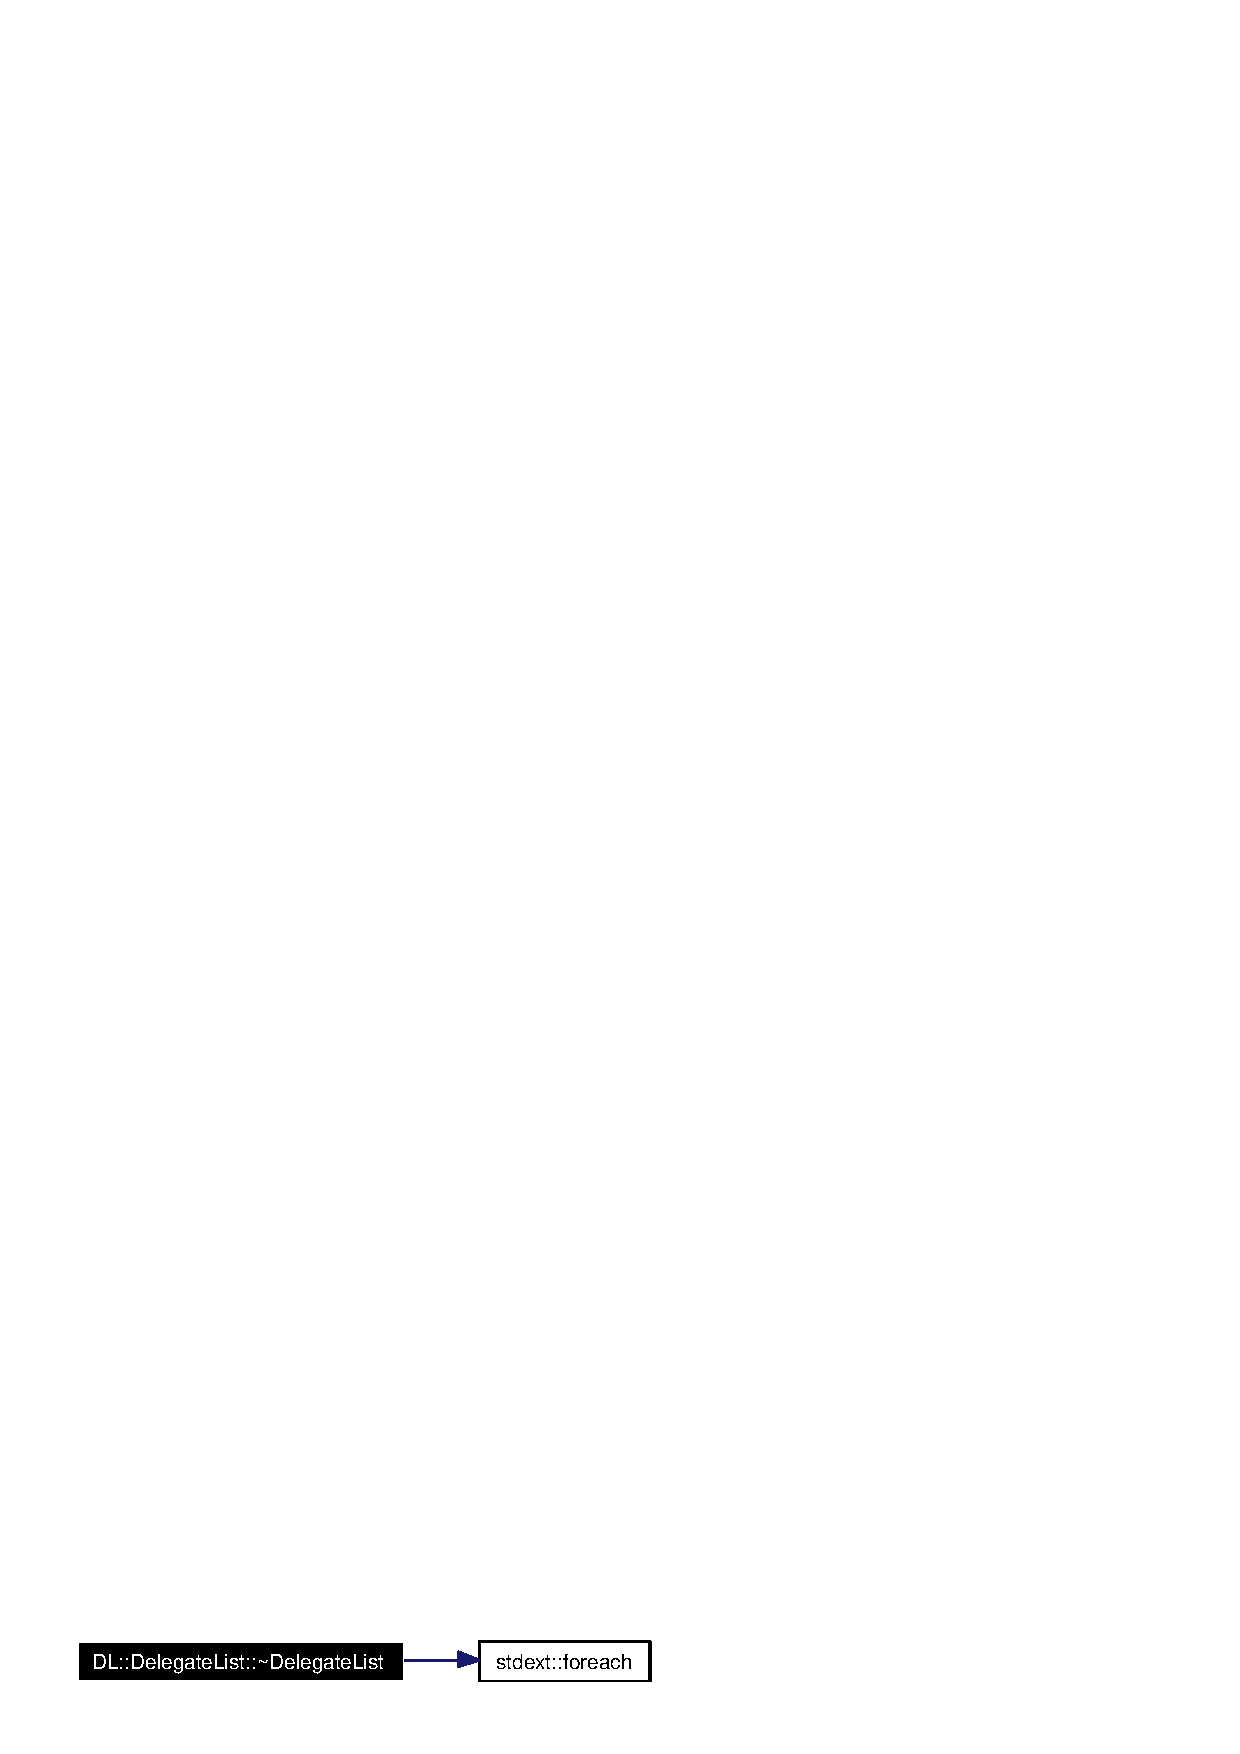
\includegraphics[width=156pt]{classDL_1_1DelegateList_a0_cgraph}
\end{center}
\end{figure}


\subsection{Member Function Documentation}
\hypertarget{classDL_1_1DelegateList_a1}{
\index{DL::DelegateList@{DL::Delegate\-List}!add@{add}}
\index{add@{add}!DL::DelegateList@{DL::Delegate\-List}}
\subsubsection[add]{\setlength{\rightskip}{0pt plus 5cm}void DL::Delegate\-List::add (\hyperlink{namespaceDL_a0}{Delegate\-Obj} {\em m\_\-obj})\hspace{0.3cm}{\tt  \mbox{[}inline\mbox{]}}}}
\label{classDL_1_1DelegateList_a1}




Definition at line 36 of file Delegate\-List.hpp.

References m\_\-obj\_\-list.

Referenced by main().\hypertarget{classDL_1_1DelegateList_a3}{
\index{DL::DelegateList@{DL::Delegate\-List}!call@{call}}
\index{call@{call}!DL::DelegateList@{DL::Delegate\-List}}
\subsubsection[call]{\setlength{\rightskip}{0pt plus 5cm}void DL::Delegate\-List::call ()\hspace{0.3cm}{\tt  \mbox{[}inline\mbox{]}}}}
\label{classDL_1_1DelegateList_a3}




Definition at line 44 of file Delegate\-List.hpp.

References stdext::foreach(), and m\_\-obj\_\-list.

Referenced by main().

Here is the call graph for this function:\begin{figure}[H]
\begin{center}
\leavevmode
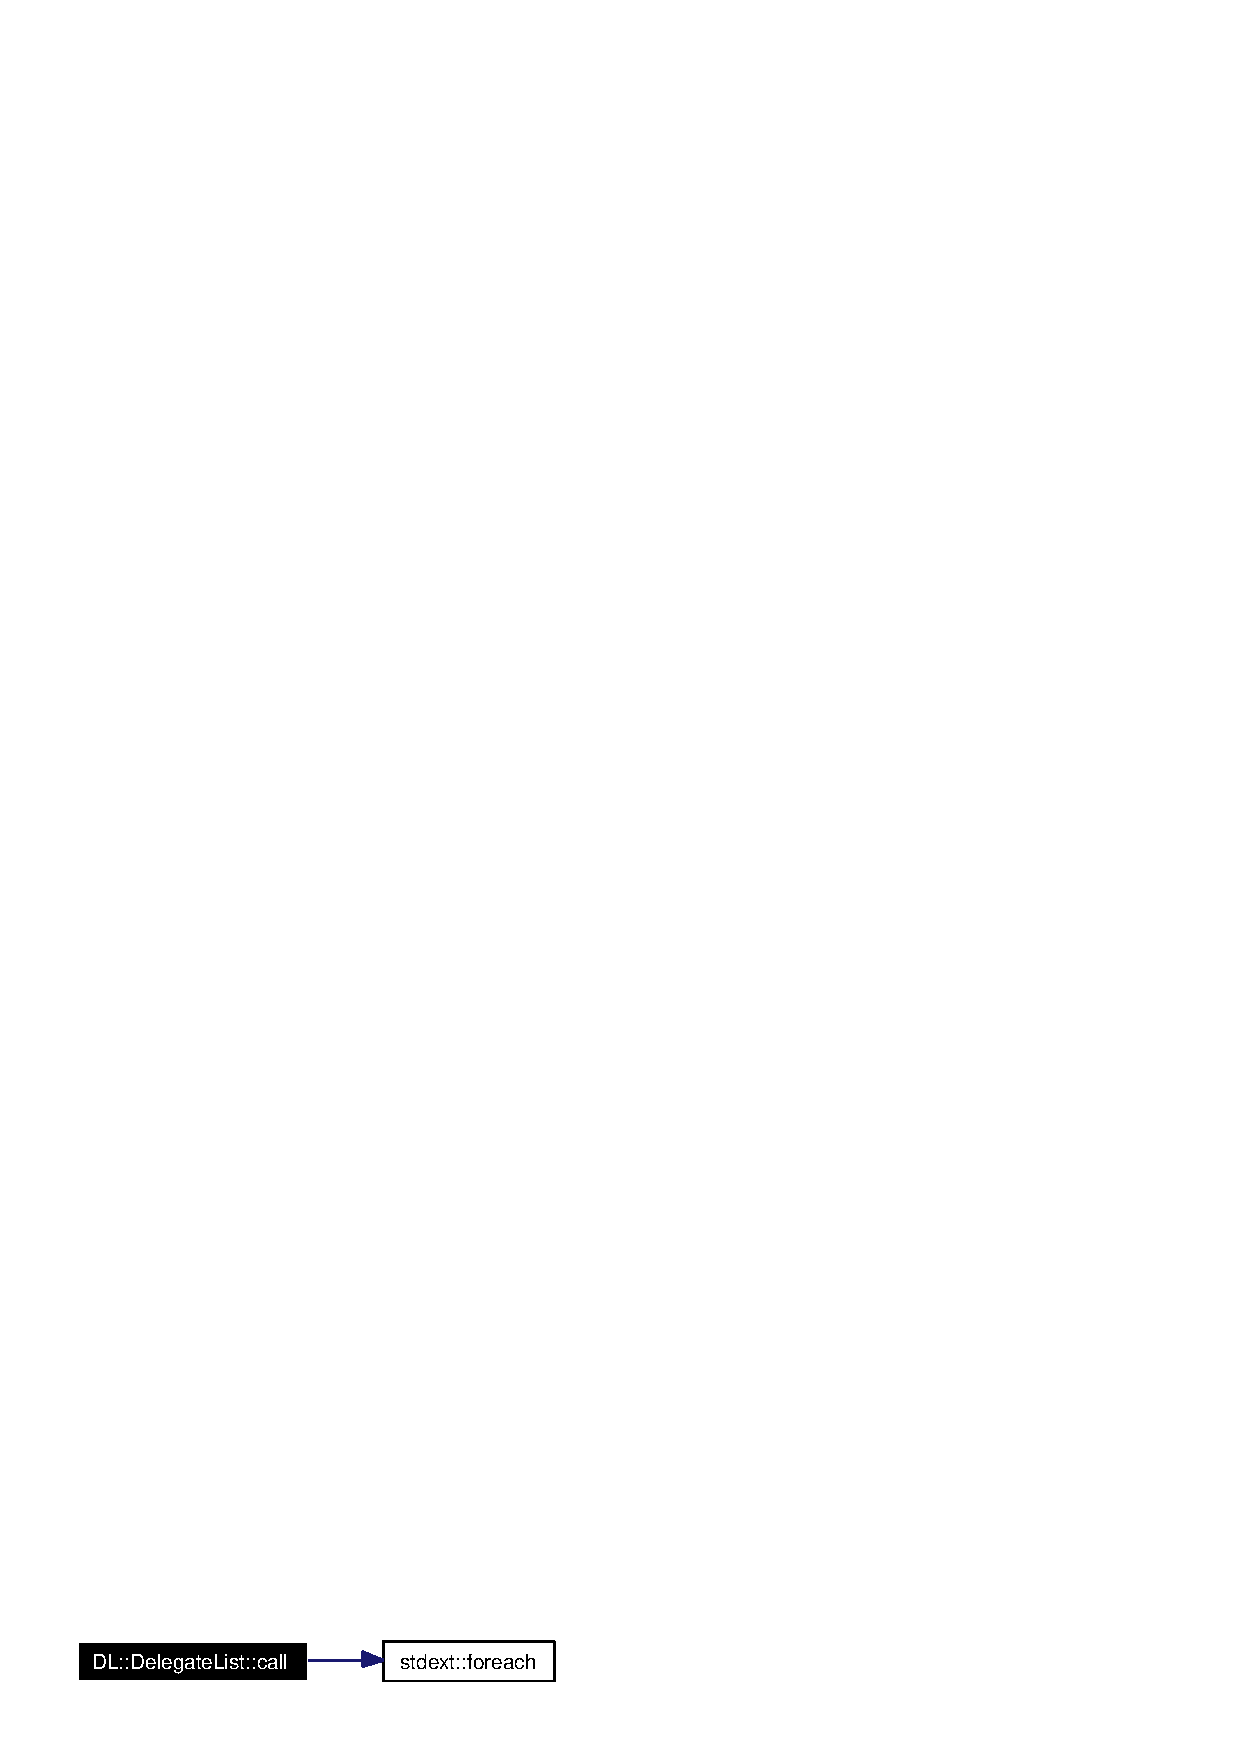
\includegraphics[width=133pt]{classDL_1_1DelegateList_a3_cgraph}
\end{center}
\end{figure}
\hypertarget{classDL_1_1DelegateList_a4}{
\index{DL::DelegateList@{DL::Delegate\-List}!operator()@{operator()}}
\index{operator()@{operator()}!DL::DelegateList@{DL::Delegate\-List}}
\subsubsection[operator()]{\setlength{\rightskip}{0pt plus 5cm}void DL::Delegate\-List::operator() ()\hspace{0.3cm}{\tt  \mbox{[}inline\mbox{]}}}}
\label{classDL_1_1DelegateList_a4}


\hyperlink{classDL_1_1DelegateList_a4}{Delegate\-List::operator()()} is used to emits all stored Delegates$<$$>$

Definition at line 50 of file Delegate\-List.hpp.

References stdext::foreach(), and m\_\-obj\_\-list.

Here is the call graph for this function:\begin{figure}[H]
\begin{center}
\leavevmode
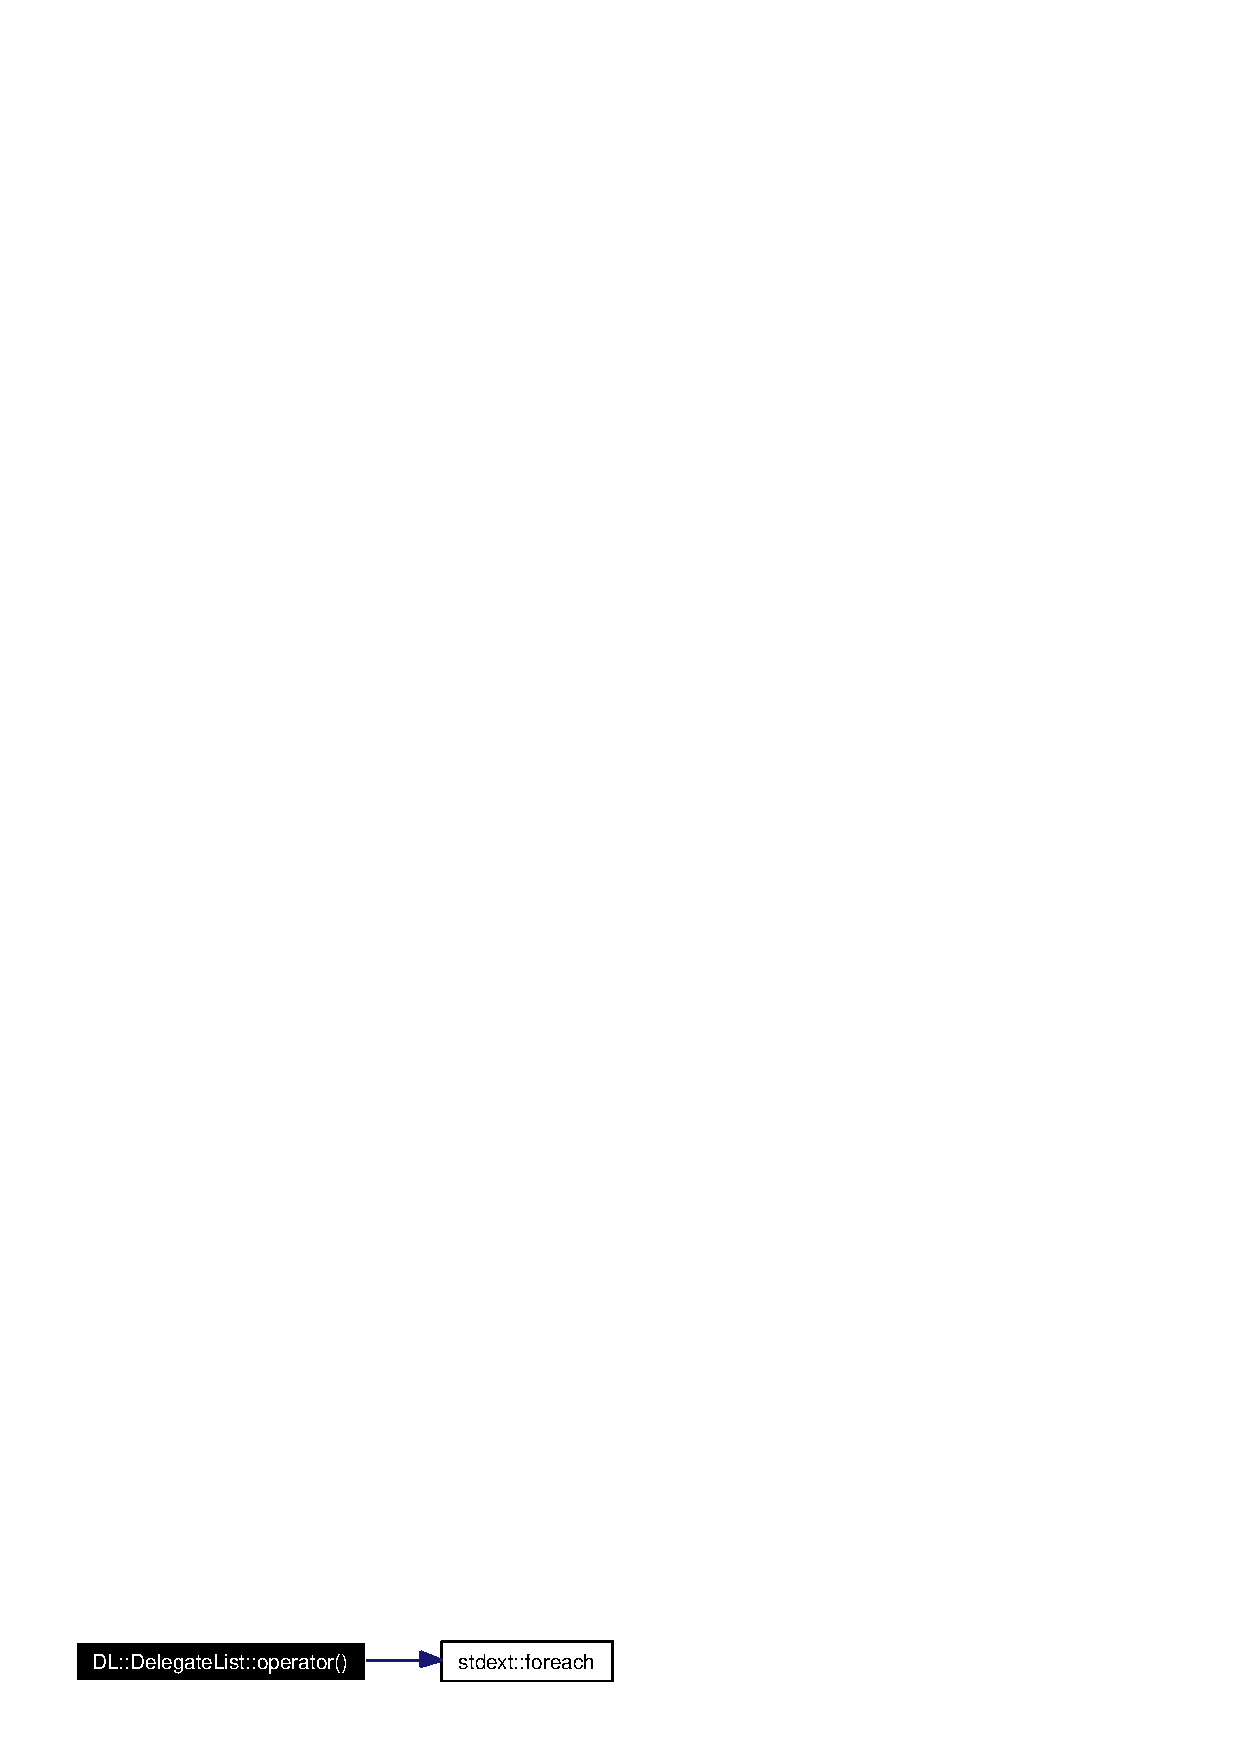
\includegraphics[width=147pt]{classDL_1_1DelegateList_a4_cgraph}
\end{center}
\end{figure}
\hypertarget{classDL_1_1DelegateList_a2}{
\index{DL::DelegateList@{DL::Delegate\-List}!reverse_call@{reverse\_\-call}}
\index{reverse_call@{reverse\_\-call}!DL::DelegateList@{DL::Delegate\-List}}
\subsubsection[reverse\_\-call]{\setlength{\rightskip}{0pt plus 5cm}void DL::Delegate\-List::reverse\_\-call ()\hspace{0.3cm}{\tt  \mbox{[}inline\mbox{]}}}}
\label{classDL_1_1DelegateList_a2}




Definition at line 40 of file Delegate\-List.hpp.

References stdext::foreach\_\-reverse(), and m\_\-obj\_\-list.

Here is the call graph for this function:\begin{figure}[H]
\begin{center}
\leavevmode
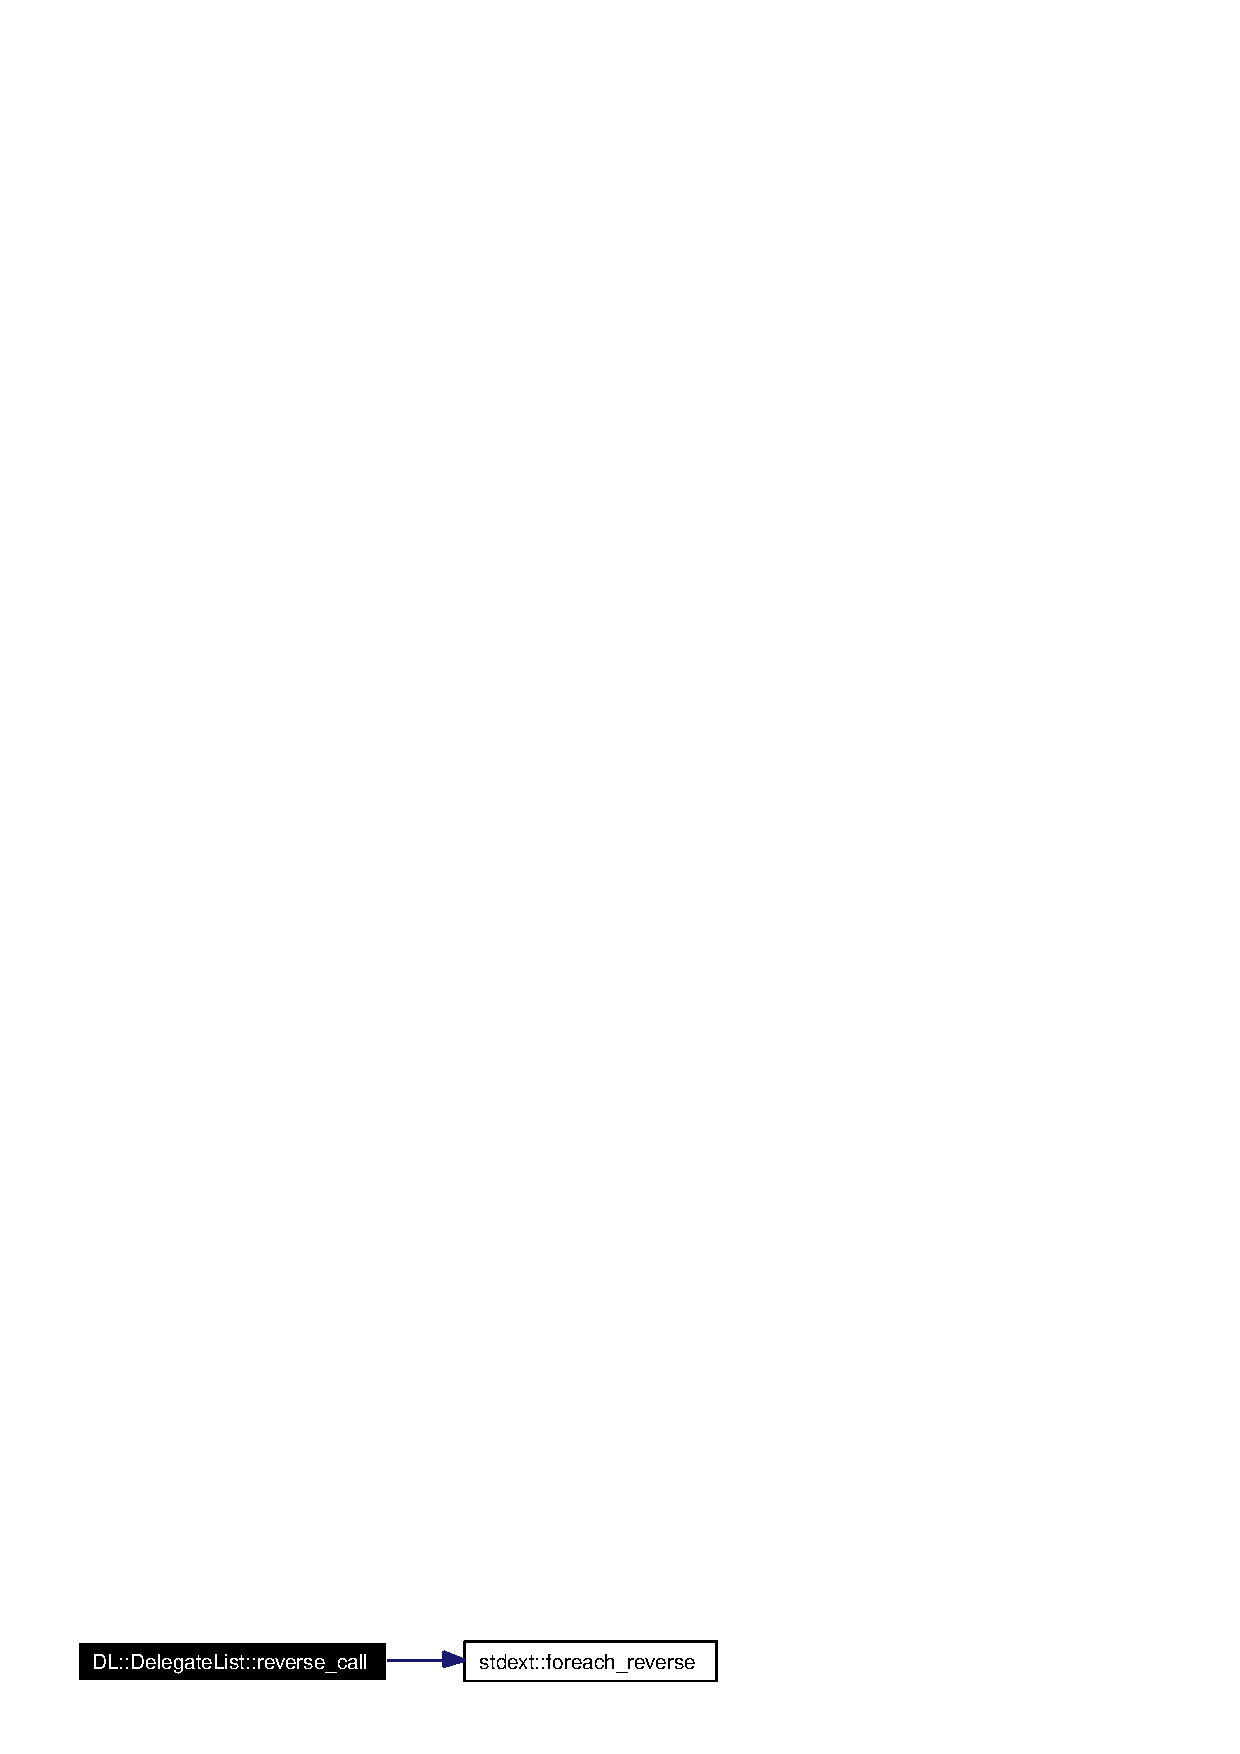
\includegraphics[width=172pt]{classDL_1_1DelegateList_a2_cgraph}
\end{center}
\end{figure}


\subsection{Member Data Documentation}
\hypertarget{classDL_1_1DelegateList_r0}{
\index{DL::DelegateList@{DL::Delegate\-List}!m_obj_list@{m\_\-obj\_\-list}}
\index{m_obj_list@{m\_\-obj\_\-list}!DL::DelegateList@{DL::Delegate\-List}}
\subsubsection[m\_\-obj\_\-list]{\setlength{\rightskip}{0pt plus 5cm}std::deque$<$\hyperlink{classDL_1_1DelegateBase}{Delegate\-Base}$\ast$$>$ \hyperlink{classDL_1_1DelegateList_r0}{DL::Delegate\-List::m\_\-obj\_\-list}\hspace{0.3cm}{\tt  \mbox{[}private\mbox{]}}}}
\label{classDL_1_1DelegateList_r0}




Definition at line 55 of file Delegate\-List.hpp.

Referenced by add(), call(), operator()(), reverse\_\-call(), and $\sim$Delegate\-List().

The documentation for this class was generated from the following file:\begin{CompactItemize}
\item 
/data/callbackext/Container/\hyperlink{DelegateList_8hpp}{Delegate\-List.hpp}\end{CompactItemize}

\hypertarget{structDL_1_1Deleter}{
\section{DL::Deleter$<$ Map\-Type $>$ Struct Template Reference}
\label{structDL_1_1Deleter}\index{DL::Deleter@{DL::Deleter}}
}
{\tt \#include $<$Associative.hpp$>$}

\subsection*{Public Member Functions}
\begin{CompactItemize}
\item 
void \hyperlink{structDL_1_1Deleter_a0}{operator()} (typename Map\-Type::value\_\-type iter)
\end{CompactItemize}
\subsubsection*{template$<$class Map\-Type$>$ struct DL::Deleter$<$ Map\-Type $>$}



\subsection{Member Function Documentation}
\hypertarget{structDL_1_1Deleter_a0}{
\index{DL::Deleter@{DL::Deleter}!operator()@{operator()}}
\index{operator()@{operator()}!DL::Deleter@{DL::Deleter}}
\subsubsection[operator()]{\setlength{\rightskip}{0pt plus 5cm}template$<$class Map\-Type$>$ void \hyperlink{structDL_1_1Deleter}{DL::Deleter}$<$ Map\-Type $>$::operator() (typename Map\-Type::value\_\-type {\em iter})\hspace{0.3cm}{\tt  \mbox{[}inline\mbox{]}}}}
\label{structDL_1_1Deleter_a0}




Definition at line 31 of file Associative.hpp.

The documentation for this struct was generated from the following file:\begin{CompactItemize}
\item 
/data/callbackext/Container/\hyperlink{Associative_8hpp}{Associative.hpp}\end{CompactItemize}

\hypertarget{structFoobar}{
\section{Foobar Struct Reference}
\label{structFoobar}\index{Foobar@{Foobar}}
}
\subsection*{Public Member Functions}
\begin{CompactItemize}
\item 
void \hyperlink{structFoobar_a0}{test0} ()
\item 
void \hyperlink{structFoobar_a1}{test1} (int i1)
\item 
void \hyperlink{structFoobar_a2}{test2} (int i1, int i2)
\item 
void \hyperlink{structFoobar_a3}{test3} (int i1, int i2, int i3)
\item 
void \hyperlink{structFoobar_a4}{test4} (int i1, int i2, int i3, int i4)
\item 
void \hyperlink{structFoobar_a5}{test5} (int i1, int i2, int i3, int i4, int i5)
\item 
void \hyperlink{structFoobar_a6}{test6} (int i1, int i2, int i3, int i4, int i5, int i6)
\item 
void \hyperlink{structFoobar_a7}{test7} (int i1, int i2, int i3, int i4, int i5, int i6, int i7)
\item 
void \hyperlink{structFoobar_a8}{test8} (int i1, int i2, int i3, int i4, int i5, int i6, int i7, int i8)
\item 
void \hyperlink{structFoobar_a9}{test9} (int i1, int i2, int i3, int i4, int i5, int i6, int i7, int i8, int i9)
\item 
void \hyperlink{structFoobar_a10}{test10} (int i1, int i2, int i3, int i4, int i5, int i6, int i7, int i8, int i9, int i10)
\item 
void \hyperlink{structFoobar_a11}{test0} ()
\item 
void \hyperlink{structFoobar_a12}{test1} (int i1)
\item 
void \hyperlink{structFoobar_a13}{test2} (int i1, int i2)
\item 
void \hyperlink{structFoobar_a14}{test3} (int i1, int i2, int i3)
\item 
void \hyperlink{structFoobar_a15}{test4} (int i1, int i2, int i3, int i4)
\item 
void \hyperlink{structFoobar_a16}{test5} (int i1, int i2, int i3, int i4, int i5)
\item 
void \hyperlink{structFoobar_a17}{test6} (int i1, int i2, int i3, int i4, int i5, int i6)
\item 
void \hyperlink{structFoobar_a18}{test7} (int i1, int i2, int i3, int i4, int i5, int i6, int i7)
\item 
void \hyperlink{structFoobar_a19}{test8} (int i1, int i2, int i3, int i4, int i5, int i6, int i7, int i8)
\item 
void \hyperlink{structFoobar_a20}{test9} (int i1, int i2, int i3, int i4, int i5, int i6, int i7, int i8, int i9)
\item 
void \hyperlink{structFoobar_a21}{test10} (int i1, int i2, int i3, int i4, int i5, int i6, int i7, int i8, int i9, int i10)
\end{CompactItemize}


\subsection{Member Function Documentation}
\hypertarget{structFoobar_a11}{
\index{Foobar@{Foobar}!test0@{test0}}
\index{test0@{test0}!Foobar@{Foobar}}
\subsubsection[test0]{\setlength{\rightskip}{0pt plus 5cm}void Foobar::test0 ()\hspace{0.3cm}{\tt  \mbox{[}inline\mbox{]}}}}
\label{structFoobar_a11}




Definition at line 25 of file Delegate\-Test3.cc.\hypertarget{structFoobar_a0}{
\index{Foobar@{Foobar}!test0@{test0}}
\index{test0@{test0}!Foobar@{Foobar}}
\subsubsection[test0]{\setlength{\rightskip}{0pt plus 5cm}void Foobar::test0 ()\hspace{0.3cm}{\tt  \mbox{[}inline\mbox{]}}}}
\label{structFoobar_a0}




Definition at line 53 of file Delegate\-Test2.cc.\hypertarget{structFoobar_a12}{
\index{Foobar@{Foobar}!test1@{test1}}
\index{test1@{test1}!Foobar@{Foobar}}
\subsubsection[test1]{\setlength{\rightskip}{0pt plus 5cm}void Foobar::test1 (int {\em i1})\hspace{0.3cm}{\tt  \mbox{[}inline\mbox{]}}}}
\label{structFoobar_a12}




Definition at line 27 of file Delegate\-Test3.cc.\hypertarget{structFoobar_a1}{
\index{Foobar@{Foobar}!test1@{test1}}
\index{test1@{test1}!Foobar@{Foobar}}
\subsubsection[test1]{\setlength{\rightskip}{0pt plus 5cm}void Foobar::test1 (int {\em i1})\hspace{0.3cm}{\tt  \mbox{[}inline\mbox{]}}}}
\label{structFoobar_a1}




Definition at line 55 of file Delegate\-Test2.cc.\hypertarget{structFoobar_a21}{
\index{Foobar@{Foobar}!test10@{test10}}
\index{test10@{test10}!Foobar@{Foobar}}
\subsubsection[test10]{\setlength{\rightskip}{0pt plus 5cm}void Foobar::test10 (int {\em i1}, int {\em i2}, int {\em i3}, int {\em i4}, int {\em i5}, int {\em i6}, int {\em i7}, int {\em i8}, int {\em i9}, int {\em i10})\hspace{0.3cm}{\tt  \mbox{[}inline\mbox{]}}}}
\label{structFoobar_a21}




Definition at line 45 of file Delegate\-Test3.cc.\hypertarget{structFoobar_a10}{
\index{Foobar@{Foobar}!test10@{test10}}
\index{test10@{test10}!Foobar@{Foobar}}
\subsubsection[test10]{\setlength{\rightskip}{0pt plus 5cm}void Foobar::test10 (int {\em i1}, int {\em i2}, int {\em i3}, int {\em i4}, int {\em i5}, int {\em i6}, int {\em i7}, int {\em i8}, int {\em i9}, int {\em i10})\hspace{0.3cm}{\tt  \mbox{[}inline\mbox{]}}}}
\label{structFoobar_a10}




Definition at line 73 of file Delegate\-Test2.cc.\hypertarget{structFoobar_a13}{
\index{Foobar@{Foobar}!test2@{test2}}
\index{test2@{test2}!Foobar@{Foobar}}
\subsubsection[test2]{\setlength{\rightskip}{0pt plus 5cm}void Foobar::test2 (int {\em i1}, int {\em i2})\hspace{0.3cm}{\tt  \mbox{[}inline\mbox{]}}}}
\label{structFoobar_a13}




Definition at line 29 of file Delegate\-Test3.cc.\hypertarget{structFoobar_a2}{
\index{Foobar@{Foobar}!test2@{test2}}
\index{test2@{test2}!Foobar@{Foobar}}
\subsubsection[test2]{\setlength{\rightskip}{0pt plus 5cm}void Foobar::test2 (int {\em i1}, int {\em i2})\hspace{0.3cm}{\tt  \mbox{[}inline\mbox{]}}}}
\label{structFoobar_a2}




Definition at line 57 of file Delegate\-Test2.cc.\hypertarget{structFoobar_a14}{
\index{Foobar@{Foobar}!test3@{test3}}
\index{test3@{test3}!Foobar@{Foobar}}
\subsubsection[test3]{\setlength{\rightskip}{0pt plus 5cm}void Foobar::test3 (int {\em i1}, int {\em i2}, int {\em i3})\hspace{0.3cm}{\tt  \mbox{[}inline\mbox{]}}}}
\label{structFoobar_a14}




Definition at line 31 of file Delegate\-Test3.cc.\hypertarget{structFoobar_a3}{
\index{Foobar@{Foobar}!test3@{test3}}
\index{test3@{test3}!Foobar@{Foobar}}
\subsubsection[test3]{\setlength{\rightskip}{0pt plus 5cm}void Foobar::test3 (int {\em i1}, int {\em i2}, int {\em i3})\hspace{0.3cm}{\tt  \mbox{[}inline\mbox{]}}}}
\label{structFoobar_a3}




Definition at line 59 of file Delegate\-Test2.cc.\hypertarget{structFoobar_a15}{
\index{Foobar@{Foobar}!test4@{test4}}
\index{test4@{test4}!Foobar@{Foobar}}
\subsubsection[test4]{\setlength{\rightskip}{0pt plus 5cm}void Foobar::test4 (int {\em i1}, int {\em i2}, int {\em i3}, int {\em i4})\hspace{0.3cm}{\tt  \mbox{[}inline\mbox{]}}}}
\label{structFoobar_a15}




Definition at line 33 of file Delegate\-Test3.cc.\hypertarget{structFoobar_a4}{
\index{Foobar@{Foobar}!test4@{test4}}
\index{test4@{test4}!Foobar@{Foobar}}
\subsubsection[test4]{\setlength{\rightskip}{0pt plus 5cm}void Foobar::test4 (int {\em i1}, int {\em i2}, int {\em i3}, int {\em i4})\hspace{0.3cm}{\tt  \mbox{[}inline\mbox{]}}}}
\label{structFoobar_a4}




Definition at line 61 of file Delegate\-Test2.cc.\hypertarget{structFoobar_a16}{
\index{Foobar@{Foobar}!test5@{test5}}
\index{test5@{test5}!Foobar@{Foobar}}
\subsubsection[test5]{\setlength{\rightskip}{0pt plus 5cm}void Foobar::test5 (int {\em i1}, int {\em i2}, int {\em i3}, int {\em i4}, int {\em i5})\hspace{0.3cm}{\tt  \mbox{[}inline\mbox{]}}}}
\label{structFoobar_a16}




Definition at line 35 of file Delegate\-Test3.cc.\hypertarget{structFoobar_a5}{
\index{Foobar@{Foobar}!test5@{test5}}
\index{test5@{test5}!Foobar@{Foobar}}
\subsubsection[test5]{\setlength{\rightskip}{0pt plus 5cm}void Foobar::test5 (int {\em i1}, int {\em i2}, int {\em i3}, int {\em i4}, int {\em i5})\hspace{0.3cm}{\tt  \mbox{[}inline\mbox{]}}}}
\label{structFoobar_a5}




Definition at line 63 of file Delegate\-Test2.cc.\hypertarget{structFoobar_a17}{
\index{Foobar@{Foobar}!test6@{test6}}
\index{test6@{test6}!Foobar@{Foobar}}
\subsubsection[test6]{\setlength{\rightskip}{0pt plus 5cm}void Foobar::test6 (int {\em i1}, int {\em i2}, int {\em i3}, int {\em i4}, int {\em i5}, int {\em i6})\hspace{0.3cm}{\tt  \mbox{[}inline\mbox{]}}}}
\label{structFoobar_a17}




Definition at line 37 of file Delegate\-Test3.cc.\hypertarget{structFoobar_a6}{
\index{Foobar@{Foobar}!test6@{test6}}
\index{test6@{test6}!Foobar@{Foobar}}
\subsubsection[test6]{\setlength{\rightskip}{0pt plus 5cm}void Foobar::test6 (int {\em i1}, int {\em i2}, int {\em i3}, int {\em i4}, int {\em i5}, int {\em i6})\hspace{0.3cm}{\tt  \mbox{[}inline\mbox{]}}}}
\label{structFoobar_a6}




Definition at line 65 of file Delegate\-Test2.cc.\hypertarget{structFoobar_a18}{
\index{Foobar@{Foobar}!test7@{test7}}
\index{test7@{test7}!Foobar@{Foobar}}
\subsubsection[test7]{\setlength{\rightskip}{0pt plus 5cm}void Foobar::test7 (int {\em i1}, int {\em i2}, int {\em i3}, int {\em i4}, int {\em i5}, int {\em i6}, int {\em i7})\hspace{0.3cm}{\tt  \mbox{[}inline\mbox{]}}}}
\label{structFoobar_a18}




Definition at line 39 of file Delegate\-Test3.cc.\hypertarget{structFoobar_a7}{
\index{Foobar@{Foobar}!test7@{test7}}
\index{test7@{test7}!Foobar@{Foobar}}
\subsubsection[test7]{\setlength{\rightskip}{0pt plus 5cm}void Foobar::test7 (int {\em i1}, int {\em i2}, int {\em i3}, int {\em i4}, int {\em i5}, int {\em i6}, int {\em i7})\hspace{0.3cm}{\tt  \mbox{[}inline\mbox{]}}}}
\label{structFoobar_a7}




Definition at line 67 of file Delegate\-Test2.cc.\hypertarget{structFoobar_a19}{
\index{Foobar@{Foobar}!test8@{test8}}
\index{test8@{test8}!Foobar@{Foobar}}
\subsubsection[test8]{\setlength{\rightskip}{0pt plus 5cm}void Foobar::test8 (int {\em i1}, int {\em i2}, int {\em i3}, int {\em i4}, int {\em i5}, int {\em i6}, int {\em i7}, int {\em i8})\hspace{0.3cm}{\tt  \mbox{[}inline\mbox{]}}}}
\label{structFoobar_a19}




Definition at line 41 of file Delegate\-Test3.cc.\hypertarget{structFoobar_a8}{
\index{Foobar@{Foobar}!test8@{test8}}
\index{test8@{test8}!Foobar@{Foobar}}
\subsubsection[test8]{\setlength{\rightskip}{0pt plus 5cm}void Foobar::test8 (int {\em i1}, int {\em i2}, int {\em i3}, int {\em i4}, int {\em i5}, int {\em i6}, int {\em i7}, int {\em i8})\hspace{0.3cm}{\tt  \mbox{[}inline\mbox{]}}}}
\label{structFoobar_a8}




Definition at line 69 of file Delegate\-Test2.cc.\hypertarget{structFoobar_a20}{
\index{Foobar@{Foobar}!test9@{test9}}
\index{test9@{test9}!Foobar@{Foobar}}
\subsubsection[test9]{\setlength{\rightskip}{0pt plus 5cm}void Foobar::test9 (int {\em i1}, int {\em i2}, int {\em i3}, int {\em i4}, int {\em i5}, int {\em i6}, int {\em i7}, int {\em i8}, int {\em i9})\hspace{0.3cm}{\tt  \mbox{[}inline\mbox{]}}}}
\label{structFoobar_a20}




Definition at line 43 of file Delegate\-Test3.cc.\hypertarget{structFoobar_a9}{
\index{Foobar@{Foobar}!test9@{test9}}
\index{test9@{test9}!Foobar@{Foobar}}
\subsubsection[test9]{\setlength{\rightskip}{0pt plus 5cm}void Foobar::test9 (int {\em i1}, int {\em i2}, int {\em i3}, int {\em i4}, int {\em i5}, int {\em i6}, int {\em i7}, int {\em i8}, int {\em i9})\hspace{0.3cm}{\tt  \mbox{[}inline\mbox{]}}}}
\label{structFoobar_a9}




Definition at line 71 of file Delegate\-Test2.cc.

The documentation for this struct was generated from the following files:\begin{CompactItemize}
\item 
/data/callbackext/Tests/\hyperlink{DelegateTest2_8cc}{Delegate\-Test2.cc}\item 
/data/callbackext/Tests/\hyperlink{DelegateTest3_8cc}{Delegate\-Test3.cc}\end{CompactItemize}

\hypertarget{classDL_1_1Functor0}{
\section{DL::Functor0 Class Reference}
\label{classDL_1_1Functor0}\index{DL::Functor0@{DL::Functor0}}
}
{\tt \#include $<$Functor0.hpp$>$}

Inherits \hyperlink{classDL_1_1DelegateBase}{DL::Delegate\-Base}.

Inheritance diagram for DL::Functor0:\begin{figure}[H]
\begin{center}
\leavevmode
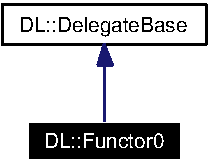
\includegraphics[width=67pt]{classDL_1_1Functor0__inherit__graph}
\end{center}
\end{figure}
Collaboration diagram for DL::Functor0:\begin{figure}[H]
\begin{center}
\leavevmode
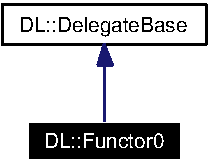
\includegraphics[width=67pt]{classDL_1_1Functor0__coll__graph}
\end{center}
\end{figure}
\subsection*{Public Member Functions}
\begin{CompactItemize}
\item 
\hyperlink{classDL_1_1Functor0_a0}{Functor0} (void($\ast$function)(void))
\item 
virtual \hyperlink{classDL_1_1Functor0_a1}{$\sim$Functor0} ()
\item 
void \hyperlink{classDL_1_1Functor0_a2}{Invoke} ()
\end{CompactItemize}
\subsection*{Private Member Functions}
\begin{CompactItemize}
\item 
\hyperlink{classDL_1_1Functor0_d0}{Functor0} ()
\end{CompactItemize}
\subsection*{Private Attributes}
\begin{CompactItemize}
\item 
void($\ast$ \hyperlink{classDL_1_1Functor0_r0}{m\_\-function} )(void)
\end{CompactItemize}


\subsection{Detailed Description}
Functor without Params



Definition at line 29 of file Functor0.hpp.

\subsection{Constructor \& Destructor Documentation}
\hypertarget{classDL_1_1Functor0_d0}{
\index{DL::Functor0@{DL::Functor0}!Functor0@{Functor0}}
\index{Functor0@{Functor0}!DL::Functor0@{DL::Functor0}}
\subsubsection[Functor0]{\setlength{\rightskip}{0pt plus 5cm}DL::Functor0::Functor0 ()\hspace{0.3cm}{\tt  \mbox{[}inline, private\mbox{]}}}}
\label{classDL_1_1Functor0_d0}




Definition at line 32 of file Functor0.hpp.\hypertarget{classDL_1_1Functor0_a0}{
\index{DL::Functor0@{DL::Functor0}!Functor0@{Functor0}}
\index{Functor0@{Functor0}!DL::Functor0@{DL::Functor0}}
\subsubsection[Functor0]{\setlength{\rightskip}{0pt plus 5cm}DL::Functor0::Functor0 (void($\ast$)(void) {\em function})\hspace{0.3cm}{\tt  \mbox{[}inline\mbox{]}}}}
\label{classDL_1_1Functor0_a0}




Definition at line 34 of file Functor0.hpp.

References m\_\-function.\hypertarget{classDL_1_1Functor0_a1}{
\index{DL::Functor0@{DL::Functor0}!~Functor0@{$\sim$Functor0}}
\index{~Functor0@{$\sim$Functor0}!DL::Functor0@{DL::Functor0}}
\subsubsection[$\sim$Functor0]{\setlength{\rightskip}{0pt plus 5cm}virtual DL::Functor0::$\sim$\hyperlink{classDL_1_1Functor0}{Functor0} ()\hspace{0.3cm}{\tt  \mbox{[}inline, virtual\mbox{]}}}}
\label{classDL_1_1Functor0_a1}




Definition at line 37 of file Functor0.hpp.

\subsection{Member Function Documentation}
\hypertarget{classDL_1_1Functor0_a2}{
\index{DL::Functor0@{DL::Functor0}!Invoke@{Invoke}}
\index{Invoke@{Invoke}!DL::Functor0@{DL::Functor0}}
\subsubsection[Invoke]{\setlength{\rightskip}{0pt plus 5cm}void DL::Functor0::Invoke ()\hspace{0.3cm}{\tt  \mbox{[}inline, virtual\mbox{]}}}}
\label{classDL_1_1Functor0_a2}




Implements \hyperlink{classDL_1_1DelegateBase_a2}{DL::Delegate\-Base}.

Definition at line 38 of file Functor0.hpp.

\subsection{Member Data Documentation}
\hypertarget{classDL_1_1Functor0_r0}{
\index{DL::Functor0@{DL::Functor0}!m_function@{m\_\-function}}
\index{m_function@{m\_\-function}!DL::Functor0@{DL::Functor0}}
\subsubsection[m\_\-function]{\setlength{\rightskip}{0pt plus 5cm}void($\ast$ \hyperlink{classDL_1_1Functor0_r0}{DL::Functor0::m\_\-function})(void)\hspace{0.3cm}{\tt  \mbox{[}private\mbox{]}}}}
\label{classDL_1_1Functor0_r0}




Referenced by Functor0().

The documentation for this class was generated from the following file:\begin{CompactItemize}
\item 
/data/callbackext/Functor\-N/\hyperlink{Functor0_8hpp}{Functor0.hpp}\end{CompactItemize}

\hypertarget{classDL_1_1Functor1}{
\section{DL::Functor1$<$ Return\-Type, Param1 $>$ Class Template Reference}
\label{classDL_1_1Functor1}\index{DL::Functor1@{DL::Functor1}}
}
{\tt \#include $<$Functor1.hpp$>$}

Inherits \hyperlink{classDL_1_1DelegateBase}{DL::Delegate\-Base}.

Inheritance diagram for DL::Functor1$<$ Return\-Type, Param1 $>$:\begin{figure}[H]
\begin{center}
\leavevmode
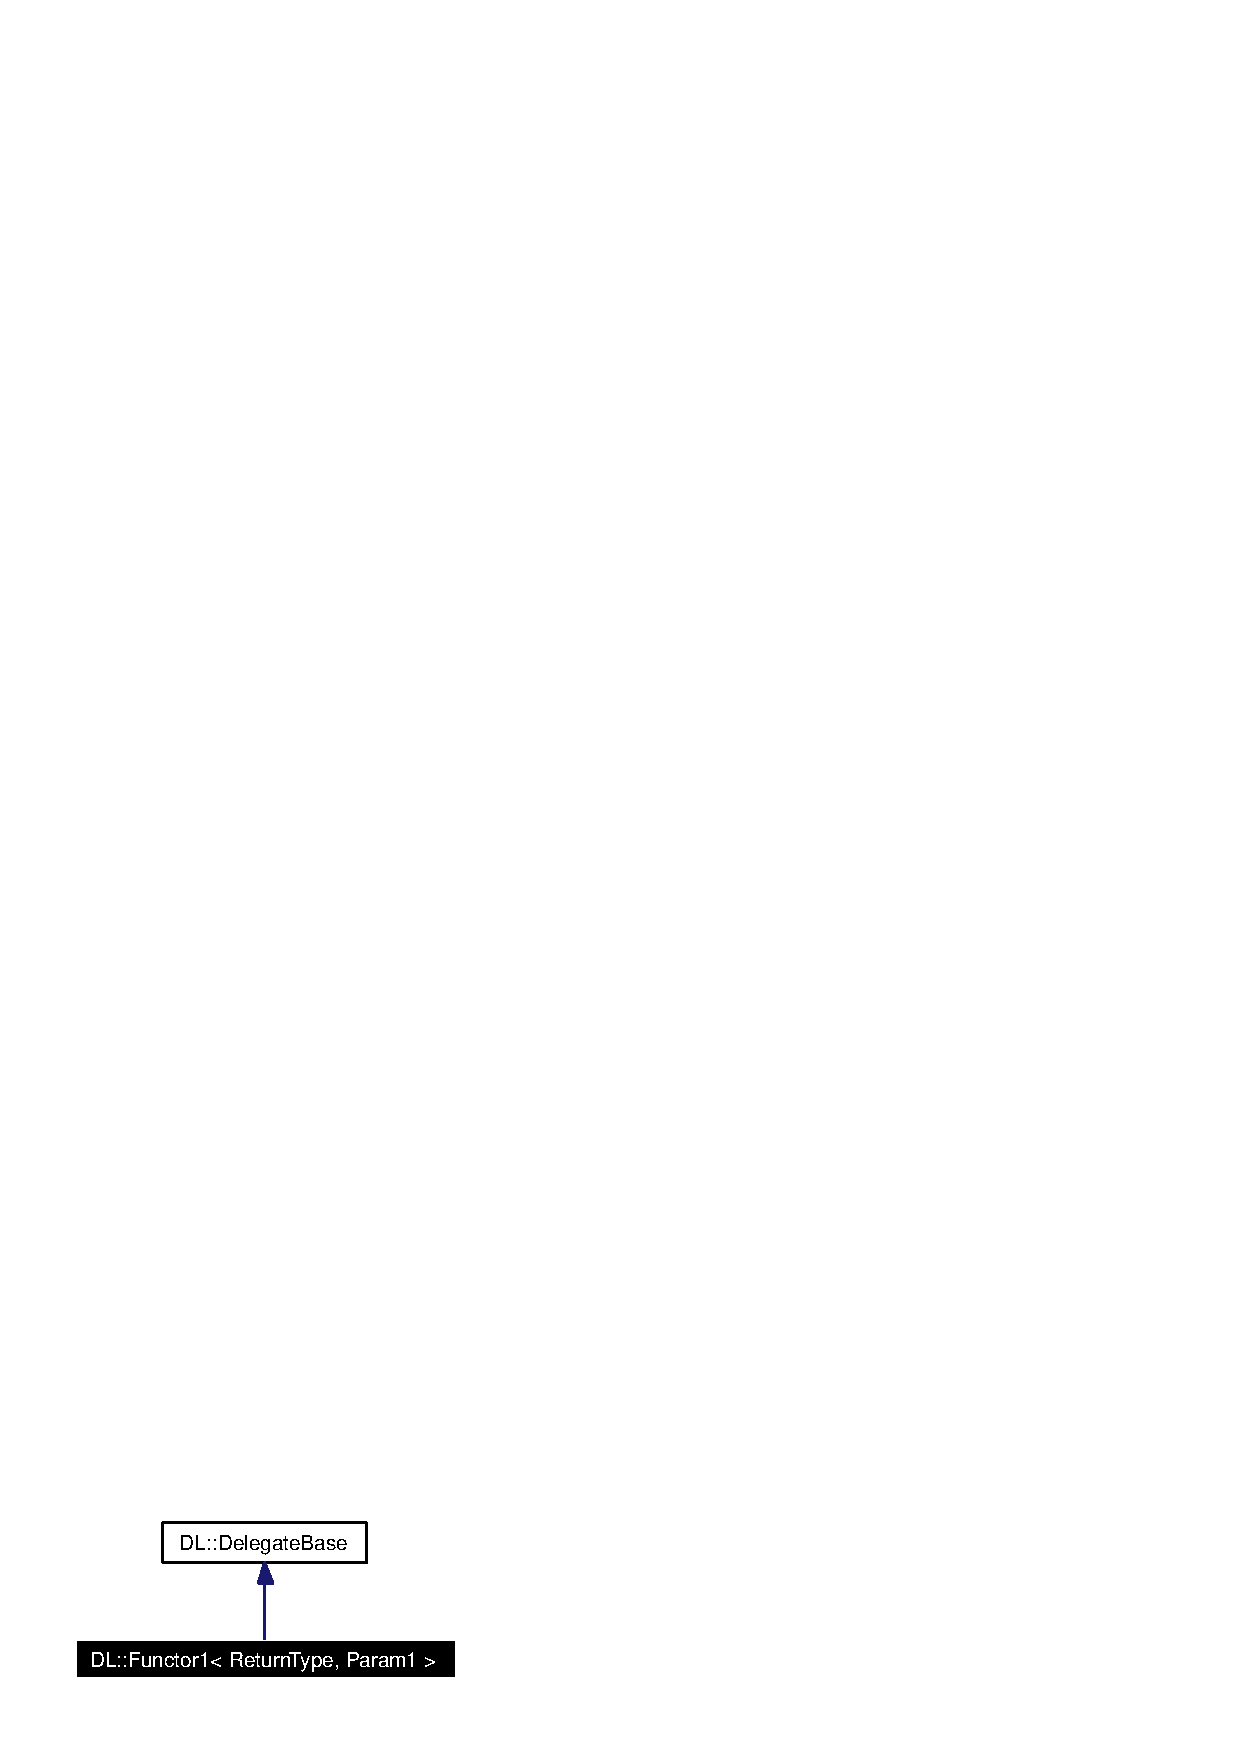
\includegraphics[width=109pt]{classDL_1_1Functor1__inherit__graph}
\end{center}
\end{figure}
Collaboration diagram for DL::Functor1$<$ Return\-Type, Param1 $>$:\begin{figure}[H]
\begin{center}
\leavevmode
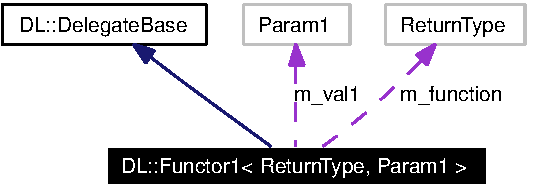
\includegraphics[width=152pt]{classDL_1_1Functor1__coll__graph}
\end{center}
\end{figure}
\subsection*{Public Member Functions}
\begin{CompactItemize}
\item 
\hyperlink{classDL_1_1Functor1_a0}{Functor1} (Return\-Type($\ast$function)(Param1), Param1 val1=Param1())
\item 
virtual \hyperlink{classDL_1_1Functor1_a1}{$\sim$Functor1} ()
\item 
void \hyperlink{classDL_1_1Functor1_a2}{Invoke} ()
\item 
Return\-Type \hyperlink{classDL_1_1Functor1_a3}{Invoke} (Param1 val1)
\end{CompactItemize}
\subsection*{Private Member Functions}
\begin{CompactItemize}
\item 
\hyperlink{classDL_1_1Functor1_d0}{Functor1} ()
\end{CompactItemize}
\subsection*{Private Attributes}
\begin{CompactItemize}
\item 
Return\-Type($\ast$ \hyperlink{classDL_1_1Functor1_r0}{m\_\-function} )(Param1)
\item 
Param1 \hyperlink{classDL_1_1Functor1_r1}{m\_\-val1}
\end{CompactItemize}


\subsection{Detailed Description}
\subsubsection*{template$<$class Return\-Type, class Param1$>$ class DL::Functor1$<$ Return\-Type, Param1 $>$}

Functor for 1 Param



Definition at line 31 of file Functor1.hpp.

\subsection{Constructor \& Destructor Documentation}
\hypertarget{classDL_1_1Functor1_d0}{
\index{DL::Functor1@{DL::Functor1}!Functor1@{Functor1}}
\index{Functor1@{Functor1}!DL::Functor1@{DL::Functor1}}
\subsubsection[Functor1]{\setlength{\rightskip}{0pt plus 5cm}template$<$class Return\-Type, class Param1$>$ \hyperlink{classDL_1_1Functor1}{DL::Functor1}$<$ Return\-Type, Param1 $>$::\hyperlink{classDL_1_1Functor1}{Functor1} ()\hspace{0.3cm}{\tt  \mbox{[}inline, private\mbox{]}}}}
\label{classDL_1_1Functor1_d0}




Definition at line 35 of file Functor1.hpp.\hypertarget{classDL_1_1Functor1_a0}{
\index{DL::Functor1@{DL::Functor1}!Functor1@{Functor1}}
\index{Functor1@{Functor1}!DL::Functor1@{DL::Functor1}}
\subsubsection[Functor1]{\setlength{\rightskip}{0pt plus 5cm}template$<$class Return\-Type, class Param1$>$ \hyperlink{classDL_1_1Functor1}{DL::Functor1}$<$ Return\-Type, Param1 $>$::\hyperlink{classDL_1_1Functor1}{Functor1} (Return\-Type($\ast$)(Param1) {\em function}, Param1 {\em val1} = {\tt Param1()})\hspace{0.3cm}{\tt  \mbox{[}inline\mbox{]}}}}
\label{classDL_1_1Functor1_a0}




Definition at line 37 of file Functor1.hpp.

References DL::Functor1$<$ Return\-Type, Param1 $>$::m\_\-function, and DL::Functor1$<$ Return\-Type, Param1 $>$::m\_\-val1.\hypertarget{classDL_1_1Functor1_a1}{
\index{DL::Functor1@{DL::Functor1}!~Functor1@{$\sim$Functor1}}
\index{~Functor1@{$\sim$Functor1}!DL::Functor1@{DL::Functor1}}
\subsubsection[$\sim$Functor1]{\setlength{\rightskip}{0pt plus 5cm}template$<$class Return\-Type, class Param1$>$ virtual \hyperlink{classDL_1_1Functor1}{DL::Functor1}$<$ Return\-Type, Param1 $>$::$\sim$\hyperlink{classDL_1_1Functor1}{Functor1} ()\hspace{0.3cm}{\tt  \mbox{[}inline, virtual\mbox{]}}}}
\label{classDL_1_1Functor1_a1}




Definition at line 41 of file Functor1.hpp.

\subsection{Member Function Documentation}
\hypertarget{classDL_1_1Functor1_a3}{
\index{DL::Functor1@{DL::Functor1}!Invoke@{Invoke}}
\index{Invoke@{Invoke}!DL::Functor1@{DL::Functor1}}
\subsubsection[Invoke]{\setlength{\rightskip}{0pt plus 5cm}template$<$class Return\-Type, class Param1$>$ Return\-Type \hyperlink{classDL_1_1Functor1}{DL::Functor1}$<$ Return\-Type, Param1 $>$::Invoke (Param1 {\em val1})\hspace{0.3cm}{\tt  \mbox{[}inline\mbox{]}}}}
\label{classDL_1_1Functor1_a3}




Definition at line 46 of file Functor1.hpp.

References DL::Functor1$<$ Return\-Type, Param1 $>$::m\_\-function.\hypertarget{classDL_1_1Functor1_a2}{
\index{DL::Functor1@{DL::Functor1}!Invoke@{Invoke}}
\index{Invoke@{Invoke}!DL::Functor1@{DL::Functor1}}
\subsubsection[Invoke]{\setlength{\rightskip}{0pt plus 5cm}template$<$class Return\-Type, class Param1$>$ void \hyperlink{classDL_1_1Functor1}{DL::Functor1}$<$ Return\-Type, Param1 $>$::Invoke ()\hspace{0.3cm}{\tt  \mbox{[}inline, virtual\mbox{]}}}}
\label{classDL_1_1Functor1_a2}




Implements \hyperlink{classDL_1_1DelegateBase_a2}{DL::Delegate\-Base}.

Definition at line 42 of file Functor1.hpp.

References DL::Functor1$<$ Return\-Type, Param1 $>$::m\_\-val1.

\subsection{Member Data Documentation}
\hypertarget{classDL_1_1Functor1_r0}{
\index{DL::Functor1@{DL::Functor1}!m_function@{m\_\-function}}
\index{m_function@{m\_\-function}!DL::Functor1@{DL::Functor1}}
\subsubsection[m\_\-function]{\setlength{\rightskip}{0pt plus 5cm}template$<$class Return\-Type, class Param1$>$ Return\-Type($\ast$ \hyperlink{classDL_1_1Functor1}{DL::Functor1}$<$ Return\-Type, Param1 $>$::\hyperlink{classDL_1_1Functor1_r0}{m\_\-function})(Param1)\hspace{0.3cm}{\tt  \mbox{[}private\mbox{]}}}}
\label{classDL_1_1Functor1_r0}




Referenced by DL::Functor1$<$ Return\-Type, Param1 $>$::Functor1(), and DL::Functor1$<$ Return\-Type, Param1 $>$::Invoke().\hypertarget{classDL_1_1Functor1_r1}{
\index{DL::Functor1@{DL::Functor1}!m_val1@{m\_\-val1}}
\index{m_val1@{m\_\-val1}!DL::Functor1@{DL::Functor1}}
\subsubsection[m\_\-val1]{\setlength{\rightskip}{0pt plus 5cm}template$<$class Return\-Type, class Param1$>$ Param1 \hyperlink{classDL_1_1Functor1}{DL::Functor1}$<$ Return\-Type, Param1 $>$::\hyperlink{classDL_1_1Functor1_r1}{m\_\-val1}\hspace{0.3cm}{\tt  \mbox{[}private\mbox{]}}}}
\label{classDL_1_1Functor1_r1}




Definition at line 34 of file Functor1.hpp.

Referenced by DL::Functor1$<$ Return\-Type, Param1 $>$::Functor1(), and DL::Functor1$<$ Return\-Type, Param1 $>$::Invoke().

The documentation for this class was generated from the following file:\begin{CompactItemize}
\item 
/data/callbackext/Functor\-N/\hyperlink{Functor1_8hpp}{Functor1.hpp}\end{CompactItemize}

\hypertarget{classDL_1_1Functor10}{
\section{DL::Functor10$<$ Return\-Type, Param1, Param2, Param3, Param4, Param5, Param6, Param7, Param8, Param9, Param10 $>$ Class Template Reference}
\label{classDL_1_1Functor10}\index{DL::Functor10@{DL::Functor10}}
}
{\tt \#include $<$Functor10.hpp$>$}

Inherits \hyperlink{classDL_1_1DelegateBase}{DL::Delegate\-Base}.

Inheritance diagram for DL::Functor10$<$ Return\-Type, Param1, Param2, Param3, Param4, Param5, Param6, Param7, Param8, Param9, Param10 $>$:\begin{figure}[H]
\begin{center}
\leavevmode
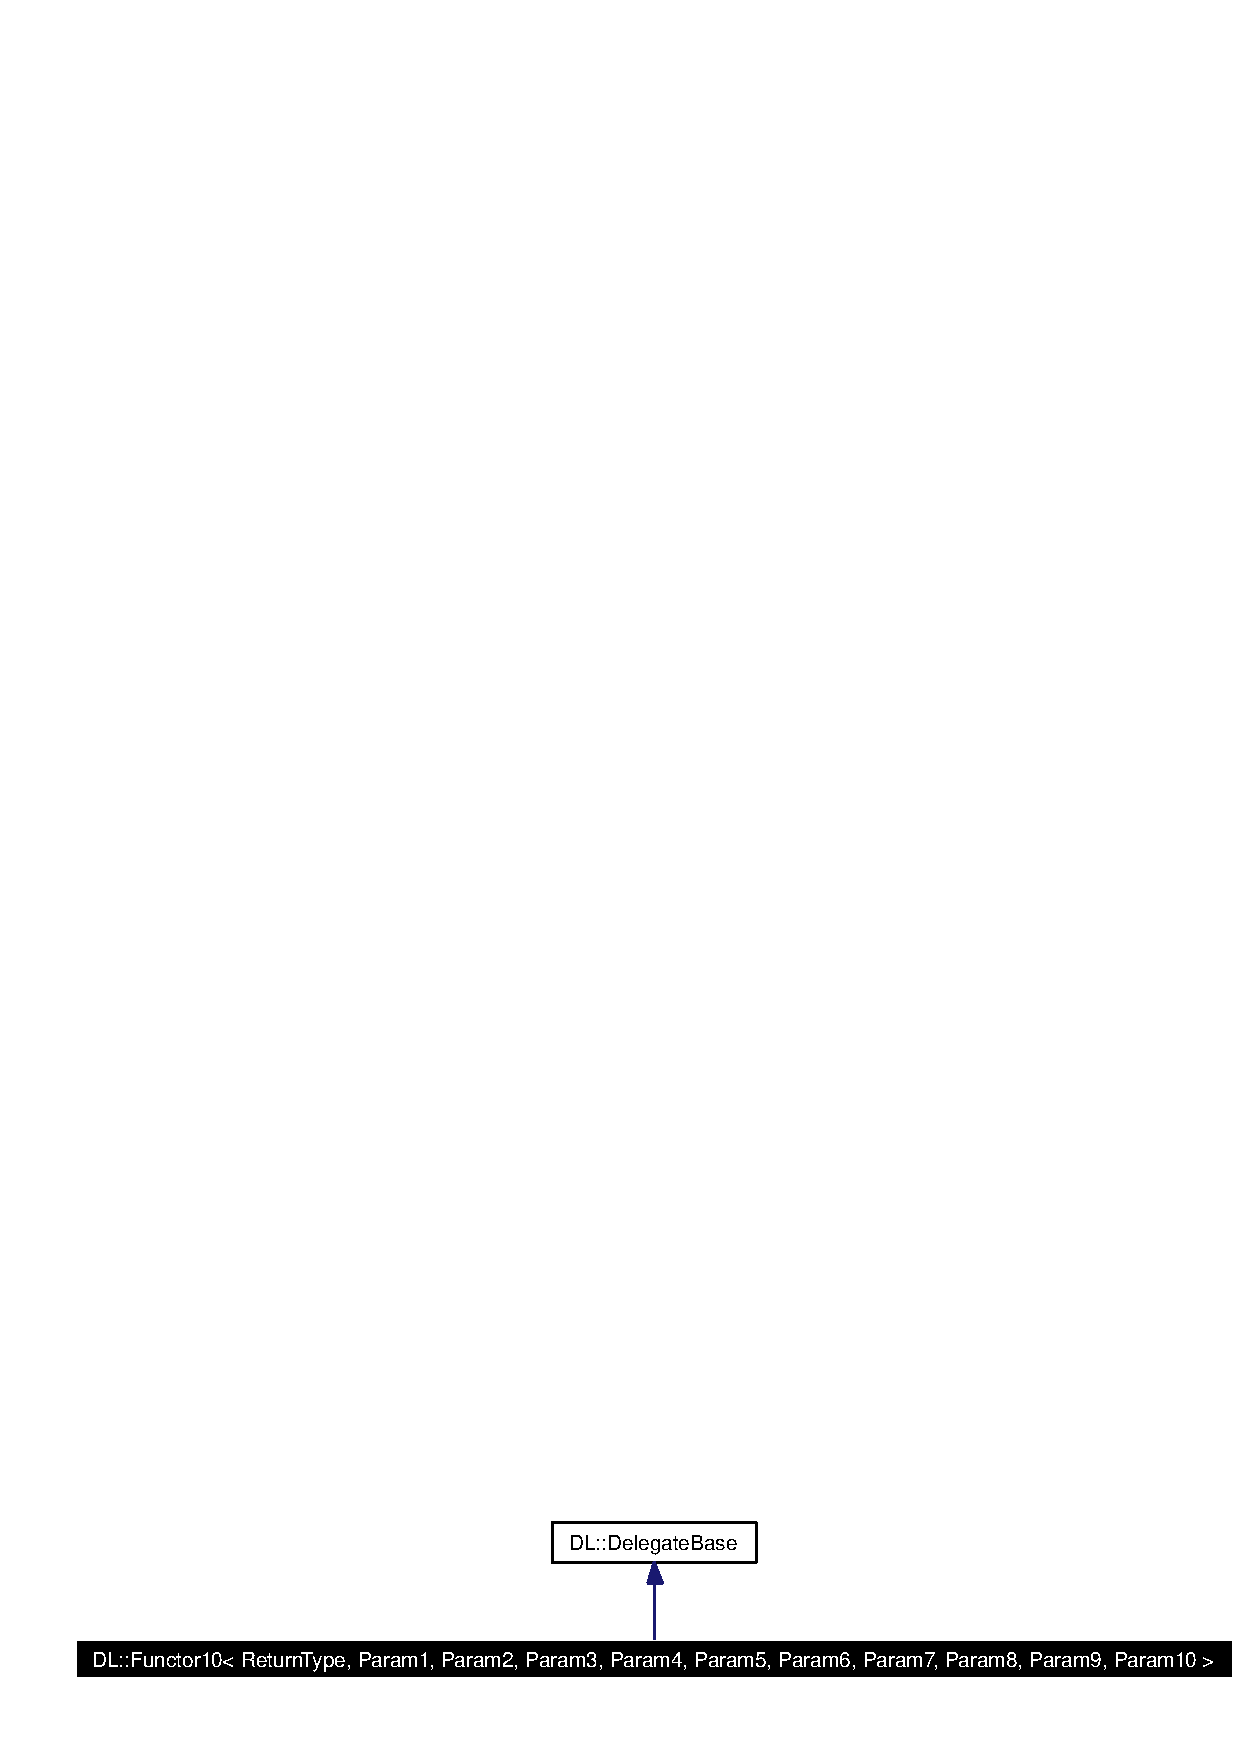
\includegraphics[width=296pt]{classDL_1_1Functor10__inherit__graph}
\end{center}
\end{figure}
Collaboration diagram for DL::Functor10$<$ Return\-Type, Param1, Param2, Param3, Param4, Param5, Param6, Param7, Param8, Param9, Param10 $>$:\begin{figure}[H]
\begin{center}
\leavevmode
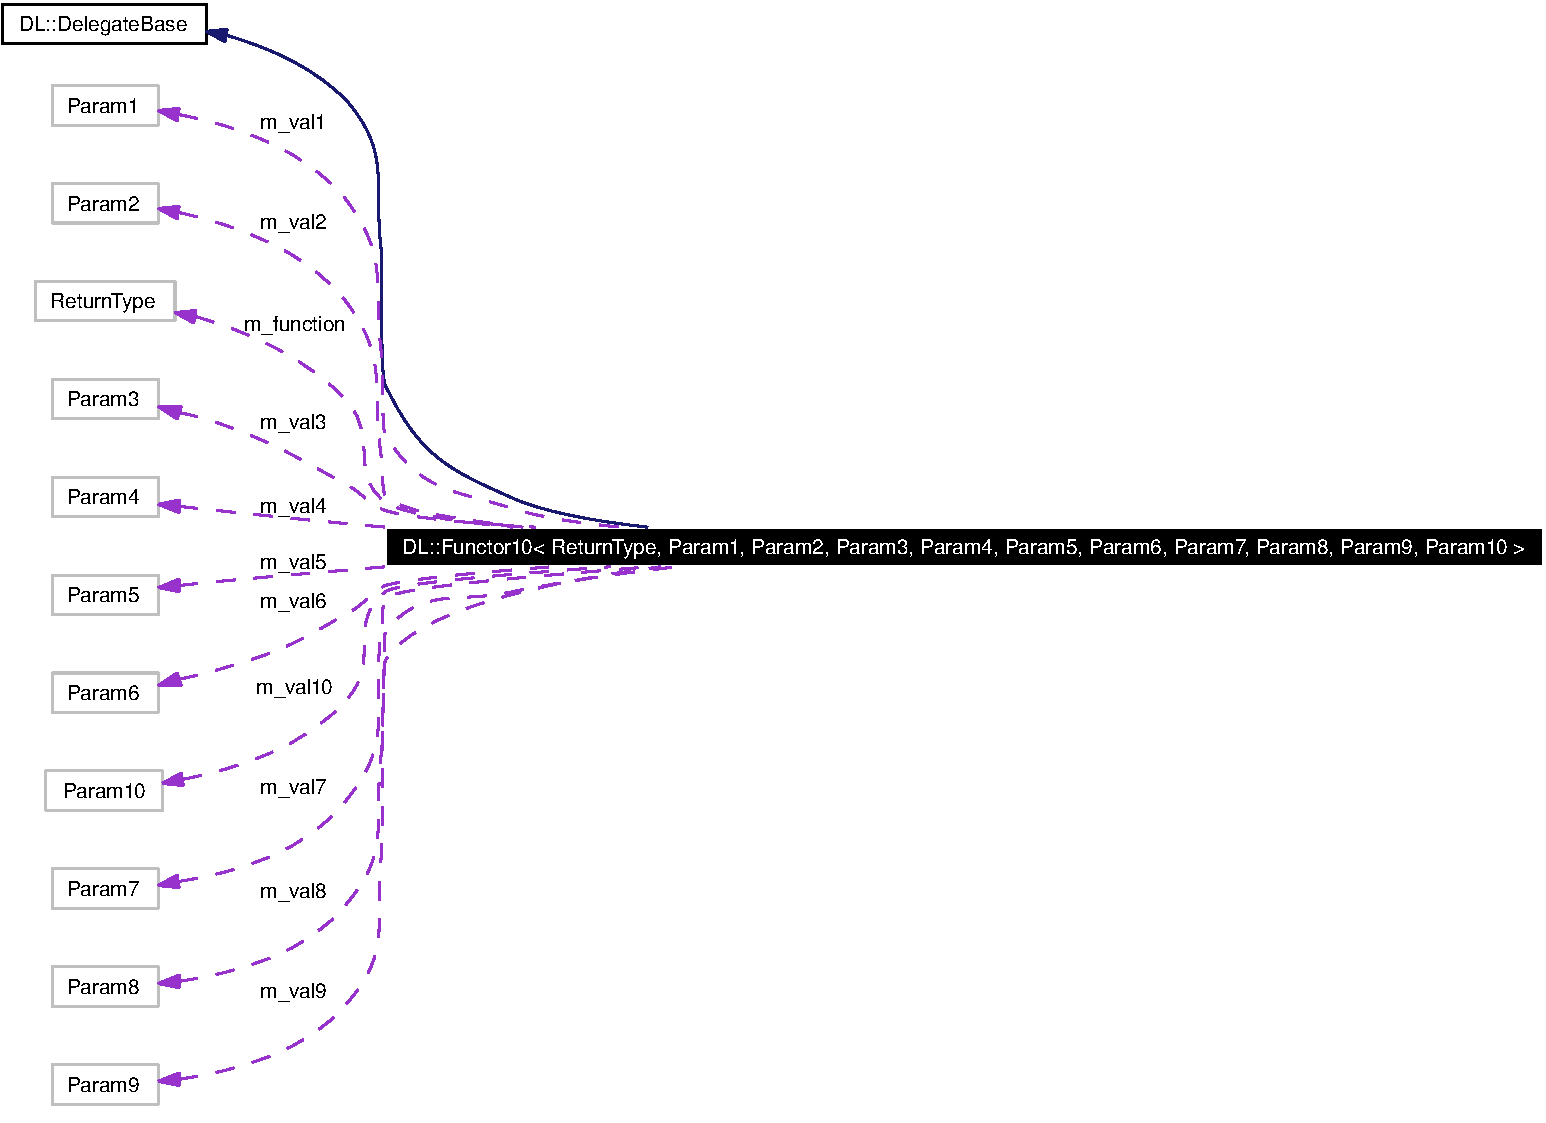
\includegraphics[width=388pt]{classDL_1_1Functor10__coll__graph}
\end{center}
\end{figure}
\subsection*{Public Member Functions}
\begin{CompactItemize}
\item 
\hyperlink{classDL_1_1Functor10_a0}{Functor10} (Return\-Type($\ast$function)(Param1, Param2, Param3, Param4, Param5, Param6, Param7, Param8, Param9, Param10), Param1 val1=Param1(), Param2 val2=Param2(), Param3 val3=Param3(), Param4 val4=Param4(), Param5 val5=Param5(), Param6 val6=Param6(), Param7 val7=Param7(), Param8 val8=Param8(), Param8 val9=Param9(), Param8 val10=Param10())
\item 
virtual \hyperlink{classDL_1_1Functor10_a1}{$\sim$Functor10} ()
\item 
void \hyperlink{classDL_1_1Functor10_a2}{Invoke} ()
\item 
Return\-Type \hyperlink{classDL_1_1Functor10_a3}{Invoke} (Param1 val1, Param2 val2, Param3 val3, Param4 val4, Param5 val5, Param6 val6, Param7 val7, Param8 val8, Param9 val9, Param10 val10)
\end{CompactItemize}
\subsection*{Private Member Functions}
\begin{CompactItemize}
\item 
\hyperlink{classDL_1_1Functor10_d0}{Functor10} ()
\end{CompactItemize}
\subsection*{Private Attributes}
\begin{CompactItemize}
\item 
Return\-Type($\ast$ \hyperlink{classDL_1_1Functor10_r0}{m\_\-function} )(Param1, Param2, Param3, Param4, Param5, Param6, Param7, Param8, Param9, Param10)
\item 
Param1 \hyperlink{classDL_1_1Functor10_r1}{m\_\-val1}
\item 
Param2 \hyperlink{classDL_1_1Functor10_r2}{m\_\-val2}
\item 
Param3 \hyperlink{classDL_1_1Functor10_r3}{m\_\-val3}
\item 
Param4 \hyperlink{classDL_1_1Functor10_r4}{m\_\-val4}
\item 
Param5 \hyperlink{classDL_1_1Functor10_r5}{m\_\-val5}
\item 
Param6 \hyperlink{classDL_1_1Functor10_r6}{m\_\-val6}
\item 
Param7 \hyperlink{classDL_1_1Functor10_r7}{m\_\-val7}
\item 
Param8 \hyperlink{classDL_1_1Functor10_r8}{m\_\-val8}
\item 
Param9 \hyperlink{classDL_1_1Functor10_r9}{m\_\-val9}
\item 
Param10 \hyperlink{classDL_1_1Functor10_r10}{m\_\-val10}
\end{CompactItemize}


\subsection{Detailed Description}
\subsubsection*{template$<$class Return\-Type, class Param1, class Param2, class Param3, class Param4, class Param5, class Param6, class Param7, class Param8, class Param9, class Param10$>$ class DL::Functor10$<$ Return\-Type, Param1, Param2, Param3, Param4, Param5, Param6, Param7, Param8, Param9, Param10 $>$}

Functor for 8 Param



Definition at line 40 of file Functor10.hpp.

\subsection{Constructor \& Destructor Documentation}
\hypertarget{classDL_1_1Functor10_d0}{
\index{DL::Functor10@{DL::Functor10}!Functor10@{Functor10}}
\index{Functor10@{Functor10}!DL::Functor10@{DL::Functor10}}
\subsubsection[Functor10]{\setlength{\rightskip}{0pt plus 5cm}template$<$class Return\-Type, class Param1, class Param2, class Param3, class Param4, class Param5, class Param6, class Param7, class Param8, class Param9, class Param10$>$ \hyperlink{classDL_1_1Functor10}{DL::Functor10}$<$ Return\-Type, Param1, Param2, Param3, Param4, Param5, Param6, Param7, Param8, Param9, Param10 $>$::\hyperlink{classDL_1_1Functor10}{Functor10} ()\hspace{0.3cm}{\tt  \mbox{[}inline, private\mbox{]}}}}
\label{classDL_1_1Functor10_d0}




Definition at line 53 of file Functor10.hpp.\hypertarget{classDL_1_1Functor10_a0}{
\index{DL::Functor10@{DL::Functor10}!Functor10@{Functor10}}
\index{Functor10@{Functor10}!DL::Functor10@{DL::Functor10}}
\subsubsection[Functor10]{\setlength{\rightskip}{0pt plus 5cm}template$<$class Return\-Type, class Param1, class Param2, class Param3, class Param4, class Param5, class Param6, class Param7, class Param8, class Param9, class Param10$>$ \hyperlink{classDL_1_1Functor10}{DL::Functor10}$<$ Return\-Type, Param1, Param2, Param3, Param4, Param5, Param6, Param7, Param8, Param9, Param10 $>$::\hyperlink{classDL_1_1Functor10}{Functor10} (Return\-Type($\ast$)(Param1, Param2, Param3, Param4, Param5, Param6, Param7, Param8, Param9, Param10) {\em function}, Param1 {\em val1} = {\tt Param1()}, Param2 {\em val2} = {\tt Param2()}, Param3 {\em val3} = {\tt Param3()}, Param4 {\em val4} = {\tt Param4()}, Param5 {\em val5} = {\tt Param5()}, Param6 {\em val6} = {\tt Param6()}, Param7 {\em val7} = {\tt Param7()}, Param8 {\em val8} = {\tt Param8()}, Param8 {\em val9} = {\tt Param9()}, Param8 {\em val10} = {\tt Param10()})\hspace{0.3cm}{\tt  \mbox{[}inline\mbox{]}}}}
\label{classDL_1_1Functor10_a0}




Definition at line 55 of file Functor10.hpp.

References DL::Functor10$<$ Return\-Type, Param1, Param2, Param3, Param4, Param5, Param6, Param7, Param8, Param9, Param10 $>$::m\_\-function, DL::Functor10$<$ Return\-Type, Param1, Param2, Param3, Param4, Param5, Param6, Param7, Param8, Param9, Param10 $>$::m\_\-val1, DL::Functor10$<$ Return\-Type, Param1, Param2, Param3, Param4, Param5, Param6, Param7, Param8, Param9, Param10 $>$::m\_\-val10, DL::Functor10$<$ Return\-Type, Param1, Param2, Param3, Param4, Param5, Param6, Param7, Param8, Param9, Param10 $>$::m\_\-val2, DL::Functor10$<$ Return\-Type, Param1, Param2, Param3, Param4, Param5, Param6, Param7, Param8, Param9, Param10 $>$::m\_\-val3, DL::Functor10$<$ Return\-Type, Param1, Param2, Param3, Param4, Param5, Param6, Param7, Param8, Param9, Param10 $>$::m\_\-val4, DL::Functor10$<$ Return\-Type, Param1, Param2, Param3, Param4, Param5, Param6, Param7, Param8, Param9, Param10 $>$::m\_\-val5, DL::Functor10$<$ Return\-Type, Param1, Param2, Param3, Param4, Param5, Param6, Param7, Param8, Param9, Param10 $>$::m\_\-val6, DL::Functor10$<$ Return\-Type, Param1, Param2, Param3, Param4, Param5, Param6, Param7, Param8, Param9, Param10 $>$::m\_\-val7, DL::Functor10$<$ Return\-Type, Param1, Param2, Param3, Param4, Param5, Param6, Param7, Param8, Param9, Param10 $>$::m\_\-val8, and DL::Functor10$<$ Return\-Type, Param1, Param2, Param3, Param4, Param5, Param6, Param7, Param8, Param9, Param10 $>$::m\_\-val9.\hypertarget{classDL_1_1Functor10_a1}{
\index{DL::Functor10@{DL::Functor10}!~Functor10@{$\sim$Functor10}}
\index{~Functor10@{$\sim$Functor10}!DL::Functor10@{DL::Functor10}}
\subsubsection[$\sim$Functor10]{\setlength{\rightskip}{0pt plus 5cm}template$<$class Return\-Type, class Param1, class Param2, class Param3, class Param4, class Param5, class Param6, class Param7, class Param8, class Param9, class Param10$>$ virtual \hyperlink{classDL_1_1Functor10}{DL::Functor10}$<$ Return\-Type, Param1, Param2, Param3, Param4, Param5, Param6, Param7, Param8, Param9, Param10 $>$::$\sim$\hyperlink{classDL_1_1Functor10}{Functor10} ()\hspace{0.3cm}{\tt  \mbox{[}inline, virtual\mbox{]}}}}
\label{classDL_1_1Functor10_a1}




Definition at line 72 of file Functor10.hpp.

\subsection{Member Function Documentation}
\hypertarget{classDL_1_1Functor10_a3}{
\index{DL::Functor10@{DL::Functor10}!Invoke@{Invoke}}
\index{Invoke@{Invoke}!DL::Functor10@{DL::Functor10}}
\subsubsection[Invoke]{\setlength{\rightskip}{0pt plus 5cm}template$<$class Return\-Type, class Param1, class Param2, class Param3, class Param4, class Param5, class Param6, class Param7, class Param8, class Param9, class Param10$>$ Return\-Type \hyperlink{classDL_1_1Functor10}{DL::Functor10}$<$ Return\-Type, Param1, Param2, Param3, Param4, Param5, Param6, Param7, Param8, Param9, Param10 $>$::Invoke (Param1 {\em val1}, Param2 {\em val2}, Param3 {\em val3}, Param4 {\em val4}, Param5 {\em val5}, Param6 {\em val6}, Param7 {\em val7}, Param8 {\em val8}, Param9 {\em val9}, Param10 {\em val10})\hspace{0.3cm}{\tt  \mbox{[}inline\mbox{]}}}}
\label{classDL_1_1Functor10_a3}




Definition at line 77 of file Functor10.hpp.\hypertarget{classDL_1_1Functor10_a2}{
\index{DL::Functor10@{DL::Functor10}!Invoke@{Invoke}}
\index{Invoke@{Invoke}!DL::Functor10@{DL::Functor10}}
\subsubsection[Invoke]{\setlength{\rightskip}{0pt plus 5cm}template$<$class Return\-Type, class Param1, class Param2, class Param3, class Param4, class Param5, class Param6, class Param7, class Param8, class Param9, class Param10$>$ void \hyperlink{classDL_1_1Functor10}{DL::Functor10}$<$ Return\-Type, Param1, Param2, Param3, Param4, Param5, Param6, Param7, Param8, Param9, Param10 $>$::Invoke ()\hspace{0.3cm}{\tt  \mbox{[}inline, virtual\mbox{]}}}}
\label{classDL_1_1Functor10_a2}




Implements \hyperlink{classDL_1_1DelegateBase_a2}{DL::Delegate\-Base}.

Definition at line 73 of file Functor10.hpp.

References DL::Functor10$<$ Return\-Type, Param1, Param2, Param3, Param4, Param5, Param6, Param7, Param8, Param9, Param10 $>$::m\_\-val1, DL::Functor10$<$ Return\-Type, Param1, Param2, Param3, Param4, Param5, Param6, Param7, Param8, Param9, Param10 $>$::m\_\-val10, DL::Functor10$<$ Return\-Type, Param1, Param2, Param3, Param4, Param5, Param6, Param7, Param8, Param9, Param10 $>$::m\_\-val2, DL::Functor10$<$ Return\-Type, Param1, Param2, Param3, Param4, Param5, Param6, Param7, Param8, Param9, Param10 $>$::m\_\-val3, DL::Functor10$<$ Return\-Type, Param1, Param2, Param3, Param4, Param5, Param6, Param7, Param8, Param9, Param10 $>$::m\_\-val4, DL::Functor10$<$ Return\-Type, Param1, Param2, Param3, Param4, Param5, Param6, Param7, Param8, Param9, Param10 $>$::m\_\-val5, DL::Functor10$<$ Return\-Type, Param1, Param2, Param3, Param4, Param5, Param6, Param7, Param8, Param9, Param10 $>$::m\_\-val6, DL::Functor10$<$ Return\-Type, Param1, Param2, Param3, Param4, Param5, Param6, Param7, Param8, Param9, Param10 $>$::m\_\-val7, DL::Functor10$<$ Return\-Type, Param1, Param2, Param3, Param4, Param5, Param6, Param7, Param8, Param9, Param10 $>$::m\_\-val8, and DL::Functor10$<$ Return\-Type, Param1, Param2, Param3, Param4, Param5, Param6, Param7, Param8, Param9, Param10 $>$::m\_\-val9.

\subsection{Member Data Documentation}
\hypertarget{classDL_1_1Functor10_r0}{
\index{DL::Functor10@{DL::Functor10}!m_function@{m\_\-function}}
\index{m_function@{m\_\-function}!DL::Functor10@{DL::Functor10}}
\subsubsection[m\_\-function]{\setlength{\rightskip}{0pt plus 5cm}template$<$class Return\-Type, class Param1, class Param2, class Param3, class Param4, class Param5, class Param6, class Param7, class Param8, class Param9, class Param10$>$ Return\-Type($\ast$ \hyperlink{classDL_1_1Functor10}{DL::Functor10}$<$ Return\-Type, Param1, Param2, Param3, Param4, Param5, Param6, Param7, Param8, Param9, Param10 $>$::\hyperlink{classDL_1_1Functor10_r0}{m\_\-function})(Param1, Param2, Param3, Param4, Param5, Param6, Param7, Param8, Param9, Param10)\hspace{0.3cm}{\tt  \mbox{[}private\mbox{]}}}}
\label{classDL_1_1Functor10_r0}




Referenced by DL::Functor10$<$ Return\-Type, Param1, Param2, Param3, Param4, Param5, Param6, Param7, Param8, Param9, Param10 $>$::Functor10().\hypertarget{classDL_1_1Functor10_r1}{
\index{DL::Functor10@{DL::Functor10}!m_val1@{m\_\-val1}}
\index{m_val1@{m\_\-val1}!DL::Functor10@{DL::Functor10}}
\subsubsection[m\_\-val1]{\setlength{\rightskip}{0pt plus 5cm}template$<$class Return\-Type, class Param1, class Param2, class Param3, class Param4, class Param5, class Param6, class Param7, class Param8, class Param9, class Param10$>$ Param1 \hyperlink{classDL_1_1Functor10}{DL::Functor10}$<$ Return\-Type, Param1, Param2, Param3, Param4, Param5, Param6, Param7, Param8, Param9, Param10 $>$::\hyperlink{classDL_1_1Functor10_r1}{m\_\-val1}\hspace{0.3cm}{\tt  \mbox{[}private\mbox{]}}}}
\label{classDL_1_1Functor10_r1}




Definition at line 43 of file Functor10.hpp.

Referenced by DL::Functor10$<$ Return\-Type, Param1, Param2, Param3, Param4, Param5, Param6, Param7, Param8, Param9, Param10 $>$::Functor10(), and DL::Functor10$<$ Return\-Type, Param1, Param2, Param3, Param4, Param5, Param6, Param7, Param8, Param9, Param10 $>$::Invoke().\hypertarget{classDL_1_1Functor10_r10}{
\index{DL::Functor10@{DL::Functor10}!m_val10@{m\_\-val10}}
\index{m_val10@{m\_\-val10}!DL::Functor10@{DL::Functor10}}
\subsubsection[m\_\-val10]{\setlength{\rightskip}{0pt plus 5cm}template$<$class Return\-Type, class Param1, class Param2, class Param3, class Param4, class Param5, class Param6, class Param7, class Param8, class Param9, class Param10$>$ Param10 \hyperlink{classDL_1_1Functor10}{DL::Functor10}$<$ Return\-Type, Param1, Param2, Param3, Param4, Param5, Param6, Param7, Param8, Param9, Param10 $>$::\hyperlink{classDL_1_1Functor10_r10}{m\_\-val10}\hspace{0.3cm}{\tt  \mbox{[}private\mbox{]}}}}
\label{classDL_1_1Functor10_r10}




Definition at line 52 of file Functor10.hpp.

Referenced by DL::Functor10$<$ Return\-Type, Param1, Param2, Param3, Param4, Param5, Param6, Param7, Param8, Param9, Param10 $>$::Functor10(), and DL::Functor10$<$ Return\-Type, Param1, Param2, Param3, Param4, Param5, Param6, Param7, Param8, Param9, Param10 $>$::Invoke().\hypertarget{classDL_1_1Functor10_r2}{
\index{DL::Functor10@{DL::Functor10}!m_val2@{m\_\-val2}}
\index{m_val2@{m\_\-val2}!DL::Functor10@{DL::Functor10}}
\subsubsection[m\_\-val2]{\setlength{\rightskip}{0pt plus 5cm}template$<$class Return\-Type, class Param1, class Param2, class Param3, class Param4, class Param5, class Param6, class Param7, class Param8, class Param9, class Param10$>$ Param2 \hyperlink{classDL_1_1Functor10}{DL::Functor10}$<$ Return\-Type, Param1, Param2, Param3, Param4, Param5, Param6, Param7, Param8, Param9, Param10 $>$::\hyperlink{classDL_1_1Functor10_r2}{m\_\-val2}\hspace{0.3cm}{\tt  \mbox{[}private\mbox{]}}}}
\label{classDL_1_1Functor10_r2}




Definition at line 44 of file Functor10.hpp.

Referenced by DL::Functor10$<$ Return\-Type, Param1, Param2, Param3, Param4, Param5, Param6, Param7, Param8, Param9, Param10 $>$::Functor10(), and DL::Functor10$<$ Return\-Type, Param1, Param2, Param3, Param4, Param5, Param6, Param7, Param8, Param9, Param10 $>$::Invoke().\hypertarget{classDL_1_1Functor10_r3}{
\index{DL::Functor10@{DL::Functor10}!m_val3@{m\_\-val3}}
\index{m_val3@{m\_\-val3}!DL::Functor10@{DL::Functor10}}
\subsubsection[m\_\-val3]{\setlength{\rightskip}{0pt plus 5cm}template$<$class Return\-Type, class Param1, class Param2, class Param3, class Param4, class Param5, class Param6, class Param7, class Param8, class Param9, class Param10$>$ Param3 \hyperlink{classDL_1_1Functor10}{DL::Functor10}$<$ Return\-Type, Param1, Param2, Param3, Param4, Param5, Param6, Param7, Param8, Param9, Param10 $>$::\hyperlink{classDL_1_1Functor10_r3}{m\_\-val3}\hspace{0.3cm}{\tt  \mbox{[}private\mbox{]}}}}
\label{classDL_1_1Functor10_r3}




Definition at line 45 of file Functor10.hpp.

Referenced by DL::Functor10$<$ Return\-Type, Param1, Param2, Param3, Param4, Param5, Param6, Param7, Param8, Param9, Param10 $>$::Functor10(), and DL::Functor10$<$ Return\-Type, Param1, Param2, Param3, Param4, Param5, Param6, Param7, Param8, Param9, Param10 $>$::Invoke().\hypertarget{classDL_1_1Functor10_r4}{
\index{DL::Functor10@{DL::Functor10}!m_val4@{m\_\-val4}}
\index{m_val4@{m\_\-val4}!DL::Functor10@{DL::Functor10}}
\subsubsection[m\_\-val4]{\setlength{\rightskip}{0pt plus 5cm}template$<$class Return\-Type, class Param1, class Param2, class Param3, class Param4, class Param5, class Param6, class Param7, class Param8, class Param9, class Param10$>$ Param4 \hyperlink{classDL_1_1Functor10}{DL::Functor10}$<$ Return\-Type, Param1, Param2, Param3, Param4, Param5, Param6, Param7, Param8, Param9, Param10 $>$::\hyperlink{classDL_1_1Functor10_r4}{m\_\-val4}\hspace{0.3cm}{\tt  \mbox{[}private\mbox{]}}}}
\label{classDL_1_1Functor10_r4}




Definition at line 46 of file Functor10.hpp.

Referenced by DL::Functor10$<$ Return\-Type, Param1, Param2, Param3, Param4, Param5, Param6, Param7, Param8, Param9, Param10 $>$::Functor10(), and DL::Functor10$<$ Return\-Type, Param1, Param2, Param3, Param4, Param5, Param6, Param7, Param8, Param9, Param10 $>$::Invoke().\hypertarget{classDL_1_1Functor10_r5}{
\index{DL::Functor10@{DL::Functor10}!m_val5@{m\_\-val5}}
\index{m_val5@{m\_\-val5}!DL::Functor10@{DL::Functor10}}
\subsubsection[m\_\-val5]{\setlength{\rightskip}{0pt plus 5cm}template$<$class Return\-Type, class Param1, class Param2, class Param3, class Param4, class Param5, class Param6, class Param7, class Param8, class Param9, class Param10$>$ Param5 \hyperlink{classDL_1_1Functor10}{DL::Functor10}$<$ Return\-Type, Param1, Param2, Param3, Param4, Param5, Param6, Param7, Param8, Param9, Param10 $>$::\hyperlink{classDL_1_1Functor10_r5}{m\_\-val5}\hspace{0.3cm}{\tt  \mbox{[}private\mbox{]}}}}
\label{classDL_1_1Functor10_r5}




Definition at line 47 of file Functor10.hpp.

Referenced by DL::Functor10$<$ Return\-Type, Param1, Param2, Param3, Param4, Param5, Param6, Param7, Param8, Param9, Param10 $>$::Functor10(), and DL::Functor10$<$ Return\-Type, Param1, Param2, Param3, Param4, Param5, Param6, Param7, Param8, Param9, Param10 $>$::Invoke().\hypertarget{classDL_1_1Functor10_r6}{
\index{DL::Functor10@{DL::Functor10}!m_val6@{m\_\-val6}}
\index{m_val6@{m\_\-val6}!DL::Functor10@{DL::Functor10}}
\subsubsection[m\_\-val6]{\setlength{\rightskip}{0pt plus 5cm}template$<$class Return\-Type, class Param1, class Param2, class Param3, class Param4, class Param5, class Param6, class Param7, class Param8, class Param9, class Param10$>$ Param6 \hyperlink{classDL_1_1Functor10}{DL::Functor10}$<$ Return\-Type, Param1, Param2, Param3, Param4, Param5, Param6, Param7, Param8, Param9, Param10 $>$::\hyperlink{classDL_1_1Functor10_r6}{m\_\-val6}\hspace{0.3cm}{\tt  \mbox{[}private\mbox{]}}}}
\label{classDL_1_1Functor10_r6}




Definition at line 48 of file Functor10.hpp.

Referenced by DL::Functor10$<$ Return\-Type, Param1, Param2, Param3, Param4, Param5, Param6, Param7, Param8, Param9, Param10 $>$::Functor10(), and DL::Functor10$<$ Return\-Type, Param1, Param2, Param3, Param4, Param5, Param6, Param7, Param8, Param9, Param10 $>$::Invoke().\hypertarget{classDL_1_1Functor10_r7}{
\index{DL::Functor10@{DL::Functor10}!m_val7@{m\_\-val7}}
\index{m_val7@{m\_\-val7}!DL::Functor10@{DL::Functor10}}
\subsubsection[m\_\-val7]{\setlength{\rightskip}{0pt plus 5cm}template$<$class Return\-Type, class Param1, class Param2, class Param3, class Param4, class Param5, class Param6, class Param7, class Param8, class Param9, class Param10$>$ Param7 \hyperlink{classDL_1_1Functor10}{DL::Functor10}$<$ Return\-Type, Param1, Param2, Param3, Param4, Param5, Param6, Param7, Param8, Param9, Param10 $>$::\hyperlink{classDL_1_1Functor10_r7}{m\_\-val7}\hspace{0.3cm}{\tt  \mbox{[}private\mbox{]}}}}
\label{classDL_1_1Functor10_r7}




Definition at line 49 of file Functor10.hpp.

Referenced by DL::Functor10$<$ Return\-Type, Param1, Param2, Param3, Param4, Param5, Param6, Param7, Param8, Param9, Param10 $>$::Functor10(), and DL::Functor10$<$ Return\-Type, Param1, Param2, Param3, Param4, Param5, Param6, Param7, Param8, Param9, Param10 $>$::Invoke().\hypertarget{classDL_1_1Functor10_r8}{
\index{DL::Functor10@{DL::Functor10}!m_val8@{m\_\-val8}}
\index{m_val8@{m\_\-val8}!DL::Functor10@{DL::Functor10}}
\subsubsection[m\_\-val8]{\setlength{\rightskip}{0pt plus 5cm}template$<$class Return\-Type, class Param1, class Param2, class Param3, class Param4, class Param5, class Param6, class Param7, class Param8, class Param9, class Param10$>$ Param8 \hyperlink{classDL_1_1Functor10}{DL::Functor10}$<$ Return\-Type, Param1, Param2, Param3, Param4, Param5, Param6, Param7, Param8, Param9, Param10 $>$::\hyperlink{classDL_1_1Functor10_r8}{m\_\-val8}\hspace{0.3cm}{\tt  \mbox{[}private\mbox{]}}}}
\label{classDL_1_1Functor10_r8}




Definition at line 50 of file Functor10.hpp.

Referenced by DL::Functor10$<$ Return\-Type, Param1, Param2, Param3, Param4, Param5, Param6, Param7, Param8, Param9, Param10 $>$::Functor10(), and DL::Functor10$<$ Return\-Type, Param1, Param2, Param3, Param4, Param5, Param6, Param7, Param8, Param9, Param10 $>$::Invoke().\hypertarget{classDL_1_1Functor10_r9}{
\index{DL::Functor10@{DL::Functor10}!m_val9@{m\_\-val9}}
\index{m_val9@{m\_\-val9}!DL::Functor10@{DL::Functor10}}
\subsubsection[m\_\-val9]{\setlength{\rightskip}{0pt plus 5cm}template$<$class Return\-Type, class Param1, class Param2, class Param3, class Param4, class Param5, class Param6, class Param7, class Param8, class Param9, class Param10$>$ Param9 \hyperlink{classDL_1_1Functor10}{DL::Functor10}$<$ Return\-Type, Param1, Param2, Param3, Param4, Param5, Param6, Param7, Param8, Param9, Param10 $>$::\hyperlink{classDL_1_1Functor10_r9}{m\_\-val9}\hspace{0.3cm}{\tt  \mbox{[}private\mbox{]}}}}
\label{classDL_1_1Functor10_r9}




Definition at line 51 of file Functor10.hpp.

Referenced by DL::Functor10$<$ Return\-Type, Param1, Param2, Param3, Param4, Param5, Param6, Param7, Param8, Param9, Param10 $>$::Functor10(), and DL::Functor10$<$ Return\-Type, Param1, Param2, Param3, Param4, Param5, Param6, Param7, Param8, Param9, Param10 $>$::Invoke().

The documentation for this class was generated from the following file:\begin{CompactItemize}
\item 
/data/callbackext/Functor\-N/\hyperlink{Functor10_8hpp}{Functor10.hpp}\end{CompactItemize}

\hypertarget{classDL_1_1Functor2}{
\section{DL::Functor2$<$ Return\-Type, Param1, Param2 $>$ Class Template Reference}
\label{classDL_1_1Functor2}\index{DL::Functor2@{DL::Functor2}}
}
{\tt \#include $<$Functor2.hpp$>$}

Inherits \hyperlink{classDL_1_1DelegateBase}{DL::Delegate\-Base}.

Inheritance diagram for DL::Functor2$<$ Return\-Type, Param1, Param2 $>$:\begin{figure}[H]
\begin{center}
\leavevmode
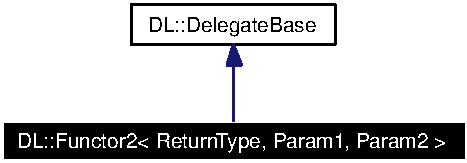
\includegraphics[width=129pt]{classDL_1_1Functor2__inherit__graph}
\end{center}
\end{figure}
Collaboration diagram for DL::Functor2$<$ Return\-Type, Param1, Param2 $>$:\begin{figure}[H]
\begin{center}
\leavevmode
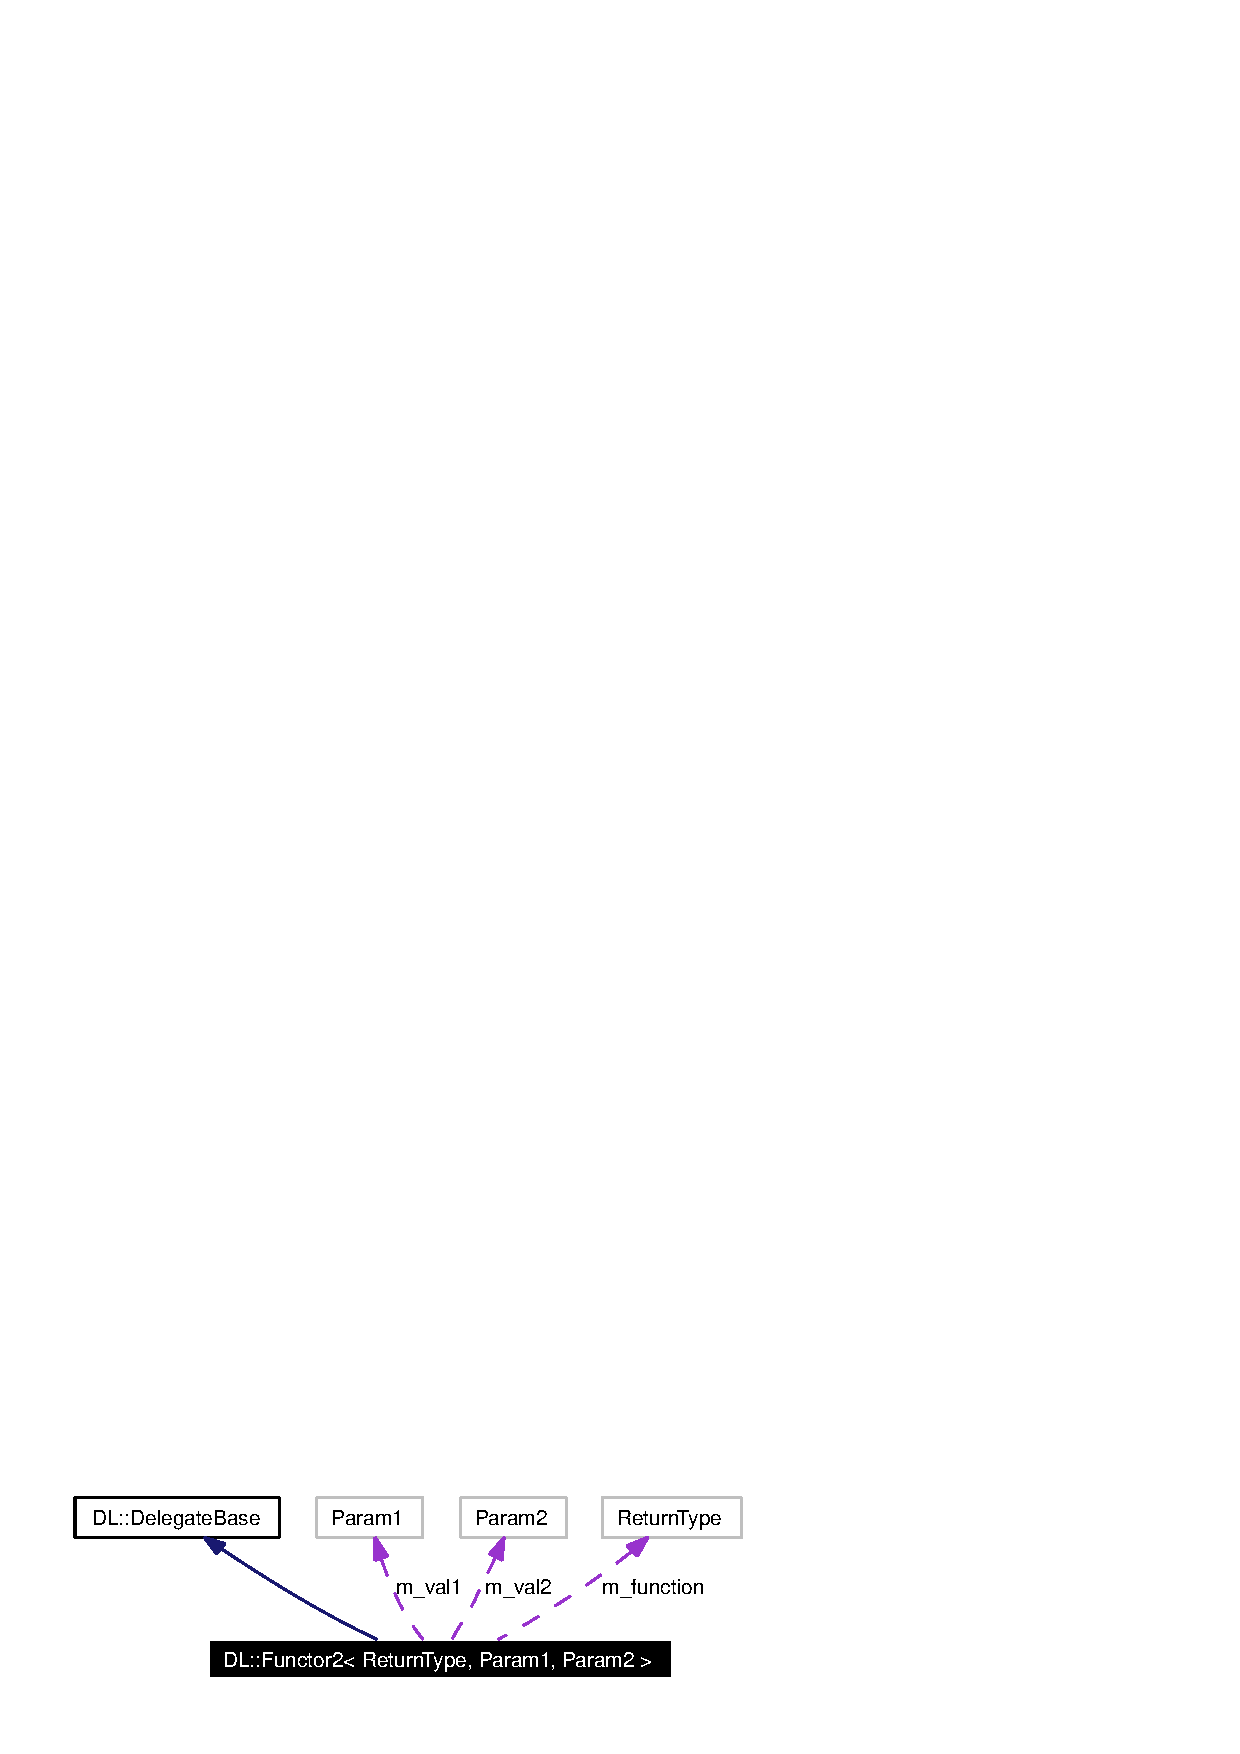
\includegraphics[width=186pt]{classDL_1_1Functor2__coll__graph}
\end{center}
\end{figure}
\subsection*{Public Member Functions}
\begin{CompactItemize}
\item 
\hyperlink{classDL_1_1Functor2_a0}{Functor2} (Return\-Type($\ast$function)(Param1, Param2), Param1 val1=Param1(), Param2 val2=Param2())
\item 
virtual \hyperlink{classDL_1_1Functor2_a1}{$\sim$Functor2} ()
\item 
void \hyperlink{classDL_1_1Functor2_a2}{Invoke} ()
\item 
Return\-Type \hyperlink{classDL_1_1Functor2_a3}{Invoke} (Param1 val1, Param2 val2)
\end{CompactItemize}
\subsection*{Private Member Functions}
\begin{CompactItemize}
\item 
\hyperlink{classDL_1_1Functor2_d0}{Functor2} ()
\end{CompactItemize}
\subsection*{Private Attributes}
\begin{CompactItemize}
\item 
Return\-Type($\ast$ \hyperlink{classDL_1_1Functor2_r0}{m\_\-function} )(Param1, Param2)
\item 
Param1 \hyperlink{classDL_1_1Functor2_r1}{m\_\-val1}
\item 
Param2 \hyperlink{classDL_1_1Functor2_r2}{m\_\-val2}
\end{CompactItemize}


\subsection{Detailed Description}
\subsubsection*{template$<$class Return\-Type, class Param1, class Param2$>$ class DL::Functor2$<$ Return\-Type, Param1, Param2 $>$}

Functor for 2 Param



Definition at line 32 of file Functor2.hpp.

\subsection{Constructor \& Destructor Documentation}
\hypertarget{classDL_1_1Functor2_d0}{
\index{DL::Functor2@{DL::Functor2}!Functor2@{Functor2}}
\index{Functor2@{Functor2}!DL::Functor2@{DL::Functor2}}
\subsubsection[Functor2]{\setlength{\rightskip}{0pt plus 5cm}template$<$class Return\-Type, class Param1, class Param2$>$ \hyperlink{classDL_1_1Functor2}{DL::Functor2}$<$ Return\-Type, Param1, Param2 $>$::\hyperlink{classDL_1_1Functor2}{Functor2} ()\hspace{0.3cm}{\tt  \mbox{[}inline, private\mbox{]}}}}
\label{classDL_1_1Functor2_d0}




Definition at line 37 of file Functor2.hpp.\hypertarget{classDL_1_1Functor2_a0}{
\index{DL::Functor2@{DL::Functor2}!Functor2@{Functor2}}
\index{Functor2@{Functor2}!DL::Functor2@{DL::Functor2}}
\subsubsection[Functor2]{\setlength{\rightskip}{0pt plus 5cm}template$<$class Return\-Type, class Param1, class Param2$>$ \hyperlink{classDL_1_1Functor2}{DL::Functor2}$<$ Return\-Type, Param1, Param2 $>$::\hyperlink{classDL_1_1Functor2}{Functor2} (Return\-Type($\ast$)(Param1, Param2) {\em function}, Param1 {\em val1} = {\tt Param1()}, Param2 {\em val2} = {\tt Param2()})\hspace{0.3cm}{\tt  \mbox{[}inline\mbox{]}}}}
\label{classDL_1_1Functor2_a0}




Definition at line 39 of file Functor2.hpp.

References DL::Functor2$<$ Return\-Type, Param1, Param2 $>$::m\_\-function, DL::Functor2$<$ Return\-Type, Param1, Param2 $>$::m\_\-val1, and DL::Functor2$<$ Return\-Type, Param1, Param2 $>$::m\_\-val2.\hypertarget{classDL_1_1Functor2_a1}{
\index{DL::Functor2@{DL::Functor2}!~Functor2@{$\sim$Functor2}}
\index{~Functor2@{$\sim$Functor2}!DL::Functor2@{DL::Functor2}}
\subsubsection[$\sim$Functor2]{\setlength{\rightskip}{0pt plus 5cm}template$<$class Return\-Type, class Param1, class Param2$>$ virtual \hyperlink{classDL_1_1Functor2}{DL::Functor2}$<$ Return\-Type, Param1, Param2 $>$::$\sim$\hyperlink{classDL_1_1Functor2}{Functor2} ()\hspace{0.3cm}{\tt  \mbox{[}inline, virtual\mbox{]}}}}
\label{classDL_1_1Functor2_a1}




Definition at line 45 of file Functor2.hpp.

\subsection{Member Function Documentation}
\hypertarget{classDL_1_1Functor2_a3}{
\index{DL::Functor2@{DL::Functor2}!Invoke@{Invoke}}
\index{Invoke@{Invoke}!DL::Functor2@{DL::Functor2}}
\subsubsection[Invoke]{\setlength{\rightskip}{0pt plus 5cm}template$<$class Return\-Type, class Param1, class Param2$>$ Return\-Type \hyperlink{classDL_1_1Functor2}{DL::Functor2}$<$ Return\-Type, Param1, Param2 $>$::Invoke (Param1 {\em val1}, Param2 {\em val2})\hspace{0.3cm}{\tt  \mbox{[}inline\mbox{]}}}}
\label{classDL_1_1Functor2_a3}




Definition at line 50 of file Functor2.hpp.

References DL::Functor2$<$ Return\-Type, Param1, Param2 $>$::m\_\-function.\hypertarget{classDL_1_1Functor2_a2}{
\index{DL::Functor2@{DL::Functor2}!Invoke@{Invoke}}
\index{Invoke@{Invoke}!DL::Functor2@{DL::Functor2}}
\subsubsection[Invoke]{\setlength{\rightskip}{0pt plus 5cm}template$<$class Return\-Type, class Param1, class Param2$>$ void \hyperlink{classDL_1_1Functor2}{DL::Functor2}$<$ Return\-Type, Param1, Param2 $>$::Invoke ()\hspace{0.3cm}{\tt  \mbox{[}inline, virtual\mbox{]}}}}
\label{classDL_1_1Functor2_a2}




Implements \hyperlink{classDL_1_1DelegateBase_a2}{DL::Delegate\-Base}.

Definition at line 46 of file Functor2.hpp.

References DL::Functor2$<$ Return\-Type, Param1, Param2 $>$::m\_\-val1, and DL::Functor2$<$ Return\-Type, Param1, Param2 $>$::m\_\-val2.

\subsection{Member Data Documentation}
\hypertarget{classDL_1_1Functor2_r0}{
\index{DL::Functor2@{DL::Functor2}!m_function@{m\_\-function}}
\index{m_function@{m\_\-function}!DL::Functor2@{DL::Functor2}}
\subsubsection[m\_\-function]{\setlength{\rightskip}{0pt plus 5cm}template$<$class Return\-Type, class Param1, class Param2$>$ Return\-Type($\ast$ \hyperlink{classDL_1_1Functor2}{DL::Functor2}$<$ Return\-Type, Param1, Param2 $>$::\hyperlink{classDL_1_1Functor2_r0}{m\_\-function})(Param1, Param2)\hspace{0.3cm}{\tt  \mbox{[}private\mbox{]}}}}
\label{classDL_1_1Functor2_r0}




Referenced by DL::Functor2$<$ Return\-Type, Param1, Param2 $>$::Functor2(), and DL::Functor2$<$ Return\-Type, Param1, Param2 $>$::Invoke().\hypertarget{classDL_1_1Functor2_r1}{
\index{DL::Functor2@{DL::Functor2}!m_val1@{m\_\-val1}}
\index{m_val1@{m\_\-val1}!DL::Functor2@{DL::Functor2}}
\subsubsection[m\_\-val1]{\setlength{\rightskip}{0pt plus 5cm}template$<$class Return\-Type, class Param1, class Param2$>$ Param1 \hyperlink{classDL_1_1Functor2}{DL::Functor2}$<$ Return\-Type, Param1, Param2 $>$::\hyperlink{classDL_1_1Functor2_r1}{m\_\-val1}\hspace{0.3cm}{\tt  \mbox{[}private\mbox{]}}}}
\label{classDL_1_1Functor2_r1}




Definition at line 35 of file Functor2.hpp.

Referenced by DL::Functor2$<$ Return\-Type, Param1, Param2 $>$::Functor2(), and DL::Functor2$<$ Return\-Type, Param1, Param2 $>$::Invoke().\hypertarget{classDL_1_1Functor2_r2}{
\index{DL::Functor2@{DL::Functor2}!m_val2@{m\_\-val2}}
\index{m_val2@{m\_\-val2}!DL::Functor2@{DL::Functor2}}
\subsubsection[m\_\-val2]{\setlength{\rightskip}{0pt plus 5cm}template$<$class Return\-Type, class Param1, class Param2$>$ Param2 \hyperlink{classDL_1_1Functor2}{DL::Functor2}$<$ Return\-Type, Param1, Param2 $>$::\hyperlink{classDL_1_1Functor2_r2}{m\_\-val2}\hspace{0.3cm}{\tt  \mbox{[}private\mbox{]}}}}
\label{classDL_1_1Functor2_r2}




Definition at line 36 of file Functor2.hpp.

Referenced by DL::Functor2$<$ Return\-Type, Param1, Param2 $>$::Functor2(), and DL::Functor2$<$ Return\-Type, Param1, Param2 $>$::Invoke().

The documentation for this class was generated from the following file:\begin{CompactItemize}
\item 
/data/callbackext/Functor\-N/\hyperlink{Functor2_8hpp}{Functor2.hpp}\end{CompactItemize}

\hypertarget{classDL_1_1Functor3}{
\section{DL::Functor3$<$ Return\-Type, Param1, Param2, Param3 $>$ Class Template Reference}
\label{classDL_1_1Functor3}\index{DL::Functor3@{DL::Functor3}}
}
{\tt \#include $<$Functor3.hpp$>$}

Inherits \hyperlink{classDL_1_1DelegateBase}{DL::Delegate\-Base}.

Inheritance diagram for DL::Functor3$<$ Return\-Type, Param1, Param2, Param3 $>$:\begin{figure}[H]
\begin{center}
\leavevmode
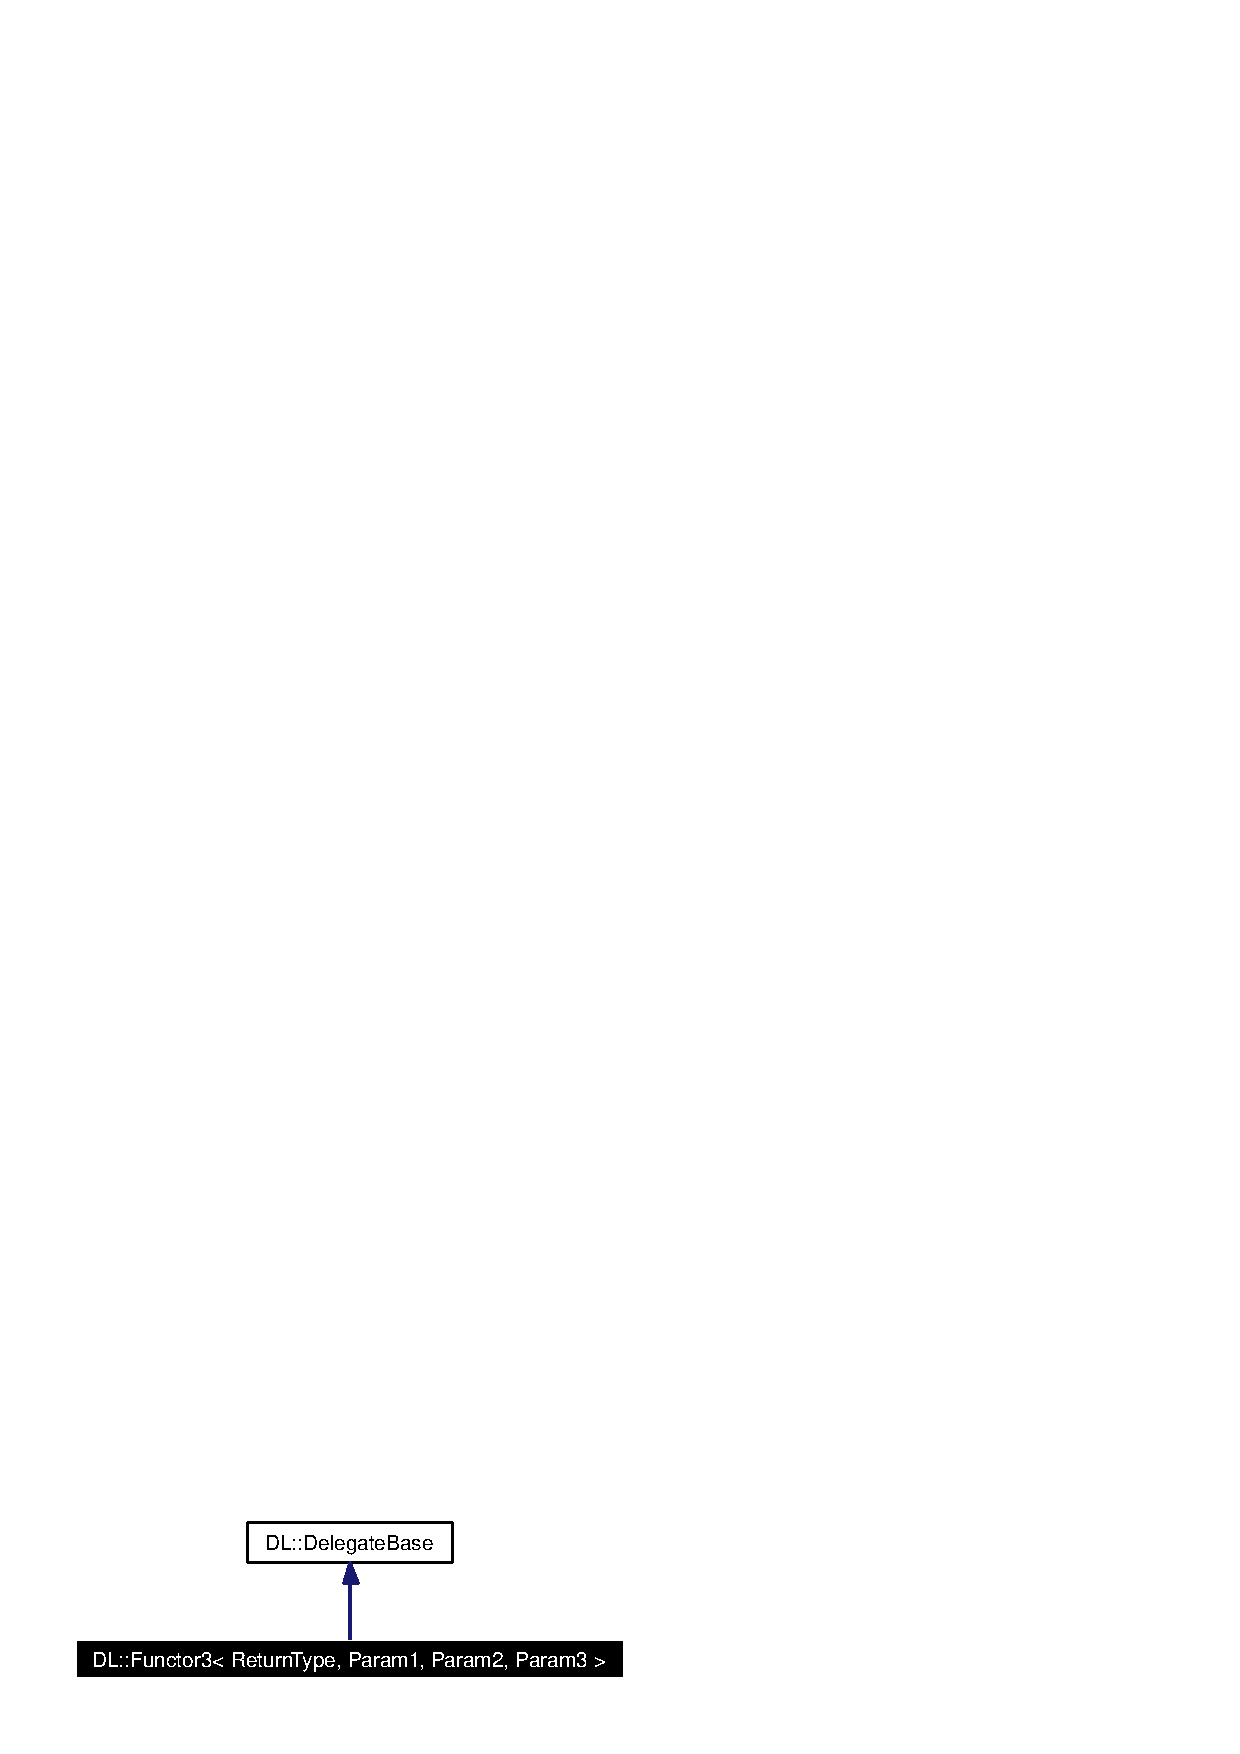
\includegraphics[width=150pt]{classDL_1_1Functor3__inherit__graph}
\end{center}
\end{figure}
Collaboration diagram for DL::Functor3$<$ Return\-Type, Param1, Param2, Param3 $>$:\begin{figure}[H]
\begin{center}
\leavevmode
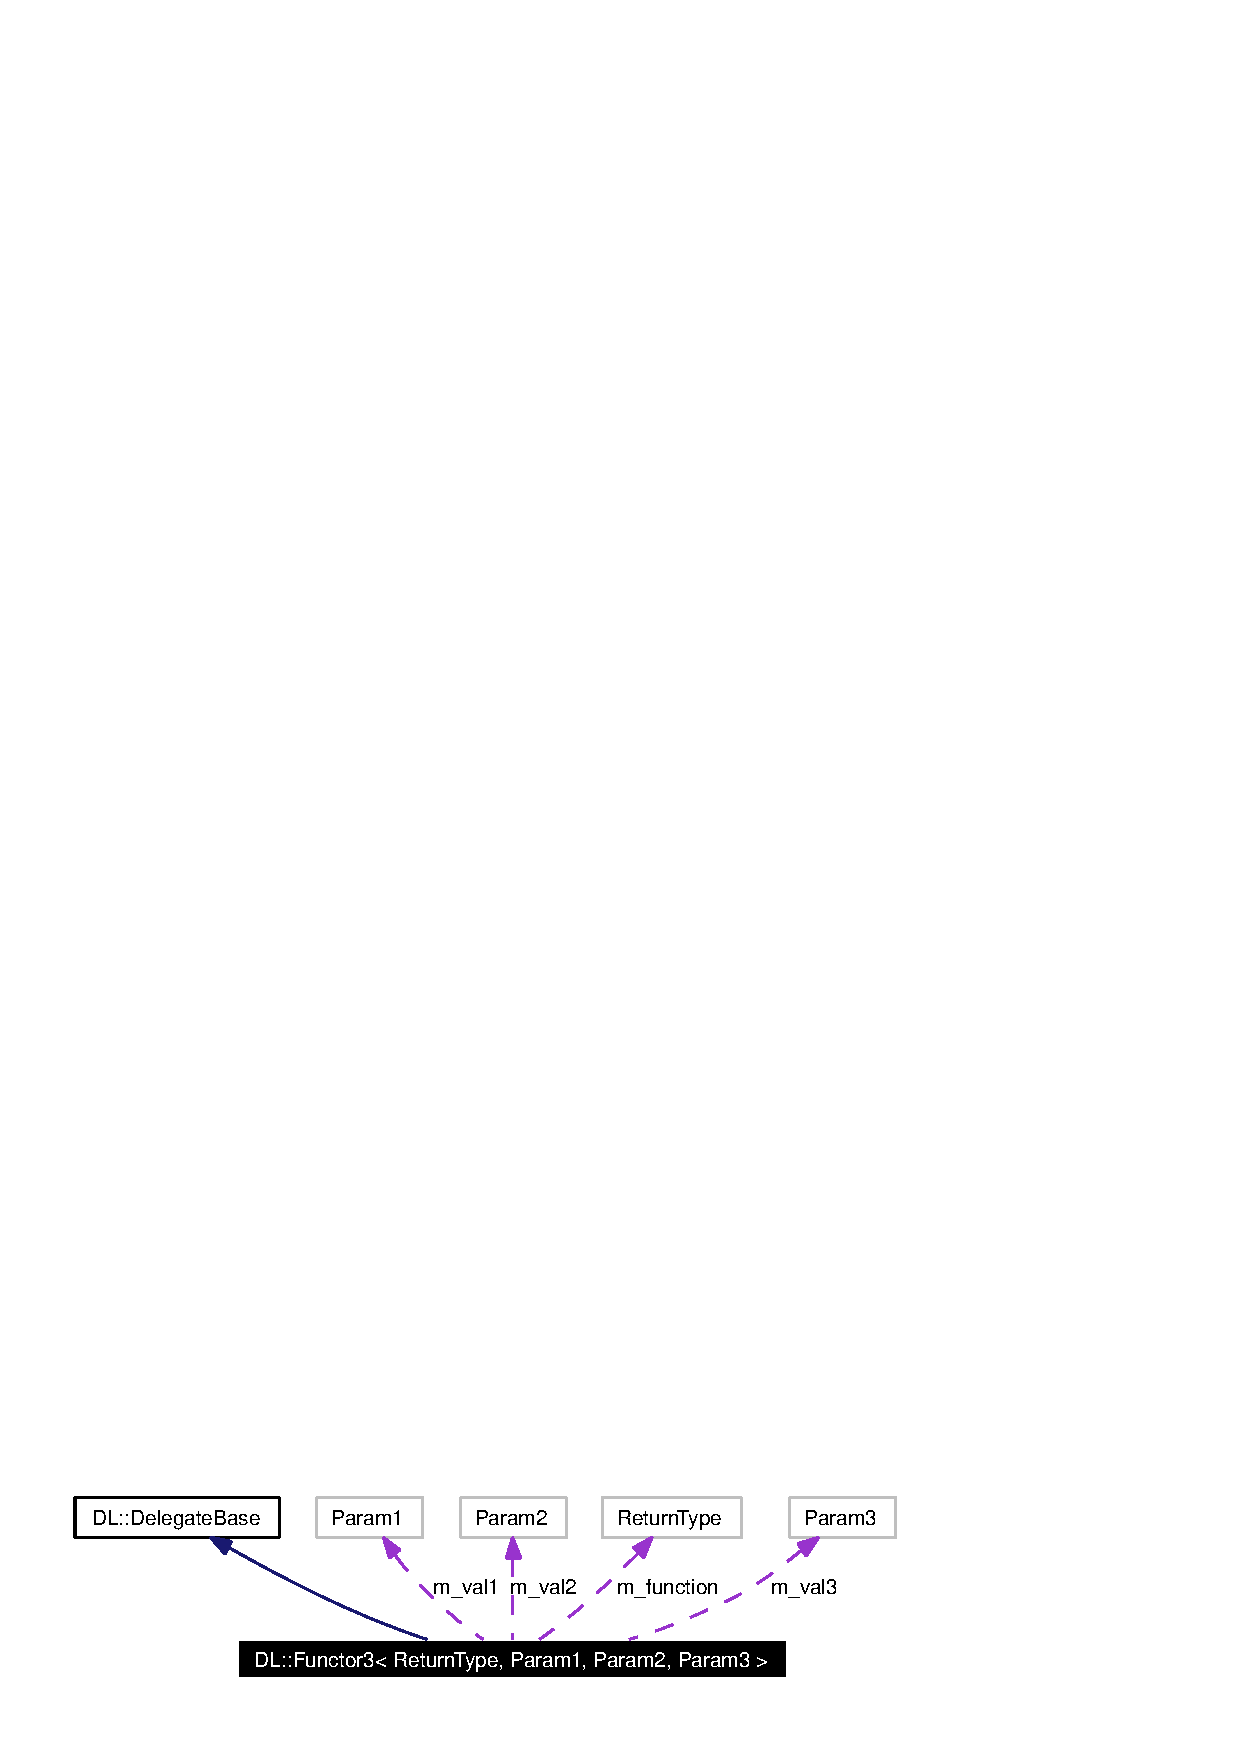
\includegraphics[width=219pt]{classDL_1_1Functor3__coll__graph}
\end{center}
\end{figure}
\subsection*{Public Member Functions}
\begin{CompactItemize}
\item 
\hyperlink{classDL_1_1Functor3_a0}{Functor3} (Return\-Type($\ast$function)(Param1, Param2, Param3), Param1 val1=Param1(), Param2 val2=Param2(), Param3 val3=Param3())
\item 
virtual \hyperlink{classDL_1_1Functor3_a1}{$\sim$Functor3} ()
\item 
void \hyperlink{classDL_1_1Functor3_a2}{Invoke} ()
\item 
Return\-Type \hyperlink{classDL_1_1Functor3_a3}{Invoke} (Param1 val1, Param2 val2, Param3 val3)
\end{CompactItemize}
\subsection*{Private Member Functions}
\begin{CompactItemize}
\item 
\hyperlink{classDL_1_1Functor3_d0}{Functor3} ()
\end{CompactItemize}
\subsection*{Private Attributes}
\begin{CompactItemize}
\item 
Return\-Type($\ast$ \hyperlink{classDL_1_1Functor3_r0}{m\_\-function} )(Param1, Param2, Param3)
\item 
Param1 \hyperlink{classDL_1_1Functor3_r1}{m\_\-val1}
\item 
Param2 \hyperlink{classDL_1_1Functor3_r2}{m\_\-val2}
\item 
Param3 \hyperlink{classDL_1_1Functor3_r3}{m\_\-val3}
\end{CompactItemize}


\subsection{Detailed Description}
\subsubsection*{template$<$class Return\-Type, class Param1, class Param2, class Param3$>$ class DL::Functor3$<$ Return\-Type, Param1, Param2, Param3 $>$}

Functor for 3 Param



Definition at line 33 of file Functor3.hpp.

\subsection{Constructor \& Destructor Documentation}
\hypertarget{classDL_1_1Functor3_d0}{
\index{DL::Functor3@{DL::Functor3}!Functor3@{Functor3}}
\index{Functor3@{Functor3}!DL::Functor3@{DL::Functor3}}
\subsubsection[Functor3]{\setlength{\rightskip}{0pt plus 5cm}template$<$class Return\-Type, class Param1, class Param2, class Param3$>$ \hyperlink{classDL_1_1Functor3}{DL::Functor3}$<$ Return\-Type, Param1, Param2, Param3 $>$::\hyperlink{classDL_1_1Functor3}{Functor3} ()\hspace{0.3cm}{\tt  \mbox{[}inline, private\mbox{]}}}}
\label{classDL_1_1Functor3_d0}




Definition at line 39 of file Functor3.hpp.\hypertarget{classDL_1_1Functor3_a0}{
\index{DL::Functor3@{DL::Functor3}!Functor3@{Functor3}}
\index{Functor3@{Functor3}!DL::Functor3@{DL::Functor3}}
\subsubsection[Functor3]{\setlength{\rightskip}{0pt plus 5cm}template$<$class Return\-Type, class Param1, class Param2, class Param3$>$ \hyperlink{classDL_1_1Functor3}{DL::Functor3}$<$ Return\-Type, Param1, Param2, Param3 $>$::\hyperlink{classDL_1_1Functor3}{Functor3} (Return\-Type($\ast$)(Param1, Param2, Param3) {\em function}, Param1 {\em val1} = {\tt Param1()}, Param2 {\em val2} = {\tt Param2()}, Param3 {\em val3} = {\tt Param3()})\hspace{0.3cm}{\tt  \mbox{[}inline\mbox{]}}}}
\label{classDL_1_1Functor3_a0}




Definition at line 41 of file Functor3.hpp.

References DL::Functor3$<$ Return\-Type, Param1, Param2, Param3 $>$::m\_\-function, DL::Functor3$<$ Return\-Type, Param1, Param2, Param3 $>$::m\_\-val1, DL::Functor3$<$ Return\-Type, Param1, Param2, Param3 $>$::m\_\-val2, and DL::Functor3$<$ Return\-Type, Param1, Param2, Param3 $>$::m\_\-val3.\hypertarget{classDL_1_1Functor3_a1}{
\index{DL::Functor3@{DL::Functor3}!~Functor3@{$\sim$Functor3}}
\index{~Functor3@{$\sim$Functor3}!DL::Functor3@{DL::Functor3}}
\subsubsection[$\sim$Functor3]{\setlength{\rightskip}{0pt plus 5cm}template$<$class Return\-Type, class Param1, class Param2, class Param3$>$ virtual \hyperlink{classDL_1_1Functor3}{DL::Functor3}$<$ Return\-Type, Param1, Param2, Param3 $>$::$\sim$\hyperlink{classDL_1_1Functor3}{Functor3} ()\hspace{0.3cm}{\tt  \mbox{[}inline, virtual\mbox{]}}}}
\label{classDL_1_1Functor3_a1}




Definition at line 48 of file Functor3.hpp.

\subsection{Member Function Documentation}
\hypertarget{classDL_1_1Functor3_a3}{
\index{DL::Functor3@{DL::Functor3}!Invoke@{Invoke}}
\index{Invoke@{Invoke}!DL::Functor3@{DL::Functor3}}
\subsubsection[Invoke]{\setlength{\rightskip}{0pt plus 5cm}template$<$class Return\-Type, class Param1, class Param2, class Param3$>$ Return\-Type \hyperlink{classDL_1_1Functor3}{DL::Functor3}$<$ Return\-Type, Param1, Param2, Param3 $>$::Invoke (Param1 {\em val1}, Param2 {\em val2}, Param3 {\em val3})\hspace{0.3cm}{\tt  \mbox{[}inline\mbox{]}}}}
\label{classDL_1_1Functor3_a3}




Definition at line 53 of file Functor3.hpp.

References DL::Functor3$<$ Return\-Type, Param1, Param2, Param3 $>$::m\_\-function.\hypertarget{classDL_1_1Functor3_a2}{
\index{DL::Functor3@{DL::Functor3}!Invoke@{Invoke}}
\index{Invoke@{Invoke}!DL::Functor3@{DL::Functor3}}
\subsubsection[Invoke]{\setlength{\rightskip}{0pt plus 5cm}template$<$class Return\-Type, class Param1, class Param2, class Param3$>$ void \hyperlink{classDL_1_1Functor3}{DL::Functor3}$<$ Return\-Type, Param1, Param2, Param3 $>$::Invoke ()\hspace{0.3cm}{\tt  \mbox{[}inline, virtual\mbox{]}}}}
\label{classDL_1_1Functor3_a2}




Implements \hyperlink{classDL_1_1DelegateBase_a2}{DL::Delegate\-Base}.

Definition at line 49 of file Functor3.hpp.

References DL::Functor3$<$ Return\-Type, Param1, Param2, Param3 $>$::m\_\-val1, DL::Functor3$<$ Return\-Type, Param1, Param2, Param3 $>$::m\_\-val2, and DL::Functor3$<$ Return\-Type, Param1, Param2, Param3 $>$::m\_\-val3.

\subsection{Member Data Documentation}
\hypertarget{classDL_1_1Functor3_r0}{
\index{DL::Functor3@{DL::Functor3}!m_function@{m\_\-function}}
\index{m_function@{m\_\-function}!DL::Functor3@{DL::Functor3}}
\subsubsection[m\_\-function]{\setlength{\rightskip}{0pt plus 5cm}template$<$class Return\-Type, class Param1, class Param2, class Param3$>$ Return\-Type($\ast$ \hyperlink{classDL_1_1Functor3}{DL::Functor3}$<$ Return\-Type, Param1, Param2, Param3 $>$::\hyperlink{classDL_1_1Functor3_r0}{m\_\-function})(Param1, Param2, Param3)\hspace{0.3cm}{\tt  \mbox{[}private\mbox{]}}}}
\label{classDL_1_1Functor3_r0}




Referenced by DL::Functor3$<$ Return\-Type, Param1, Param2, Param3 $>$::Functor3(), and DL::Functor3$<$ Return\-Type, Param1, Param2, Param3 $>$::Invoke().\hypertarget{classDL_1_1Functor3_r1}{
\index{DL::Functor3@{DL::Functor3}!m_val1@{m\_\-val1}}
\index{m_val1@{m\_\-val1}!DL::Functor3@{DL::Functor3}}
\subsubsection[m\_\-val1]{\setlength{\rightskip}{0pt plus 5cm}template$<$class Return\-Type, class Param1, class Param2, class Param3$>$ Param1 \hyperlink{classDL_1_1Functor3}{DL::Functor3}$<$ Return\-Type, Param1, Param2, Param3 $>$::\hyperlink{classDL_1_1Functor3_r1}{m\_\-val1}\hspace{0.3cm}{\tt  \mbox{[}private\mbox{]}}}}
\label{classDL_1_1Functor3_r1}




Definition at line 36 of file Functor3.hpp.

Referenced by DL::Functor3$<$ Return\-Type, Param1, Param2, Param3 $>$::Functor3(), and DL::Functor3$<$ Return\-Type, Param1, Param2, Param3 $>$::Invoke().\hypertarget{classDL_1_1Functor3_r2}{
\index{DL::Functor3@{DL::Functor3}!m_val2@{m\_\-val2}}
\index{m_val2@{m\_\-val2}!DL::Functor3@{DL::Functor3}}
\subsubsection[m\_\-val2]{\setlength{\rightskip}{0pt plus 5cm}template$<$class Return\-Type, class Param1, class Param2, class Param3$>$ Param2 \hyperlink{classDL_1_1Functor3}{DL::Functor3}$<$ Return\-Type, Param1, Param2, Param3 $>$::\hyperlink{classDL_1_1Functor3_r2}{m\_\-val2}\hspace{0.3cm}{\tt  \mbox{[}private\mbox{]}}}}
\label{classDL_1_1Functor3_r2}




Definition at line 37 of file Functor3.hpp.

Referenced by DL::Functor3$<$ Return\-Type, Param1, Param2, Param3 $>$::Functor3(), and DL::Functor3$<$ Return\-Type, Param1, Param2, Param3 $>$::Invoke().\hypertarget{classDL_1_1Functor3_r3}{
\index{DL::Functor3@{DL::Functor3}!m_val3@{m\_\-val3}}
\index{m_val3@{m\_\-val3}!DL::Functor3@{DL::Functor3}}
\subsubsection[m\_\-val3]{\setlength{\rightskip}{0pt plus 5cm}template$<$class Return\-Type, class Param1, class Param2, class Param3$>$ Param3 \hyperlink{classDL_1_1Functor3}{DL::Functor3}$<$ Return\-Type, Param1, Param2, Param3 $>$::\hyperlink{classDL_1_1Functor3_r3}{m\_\-val3}\hspace{0.3cm}{\tt  \mbox{[}private\mbox{]}}}}
\label{classDL_1_1Functor3_r3}




Definition at line 38 of file Functor3.hpp.

Referenced by DL::Functor3$<$ Return\-Type, Param1, Param2, Param3 $>$::Functor3(), and DL::Functor3$<$ Return\-Type, Param1, Param2, Param3 $>$::Invoke().

The documentation for this class was generated from the following file:\begin{CompactItemize}
\item 
/data/callbackext/Functor\-N/\hyperlink{Functor3_8hpp}{Functor3.hpp}\end{CompactItemize}

\hypertarget{classDL_1_1Functor4}{
\section{DL::Functor4$<$ Return\-Type, Param1, Param2, Param3, Param4 $>$ Class Template Reference}
\label{classDL_1_1Functor4}\index{DL::Functor4@{DL::Functor4}}
}
{\tt \#include $<$Functor4.hpp$>$}

Inherits \hyperlink{classDL_1_1DelegateBase}{DL::Delegate\-Base}.

Inheritance diagram for DL::Functor4$<$ Return\-Type, Param1, Param2, Param3, Param4 $>$:\begin{figure}[H]
\begin{center}
\leavevmode
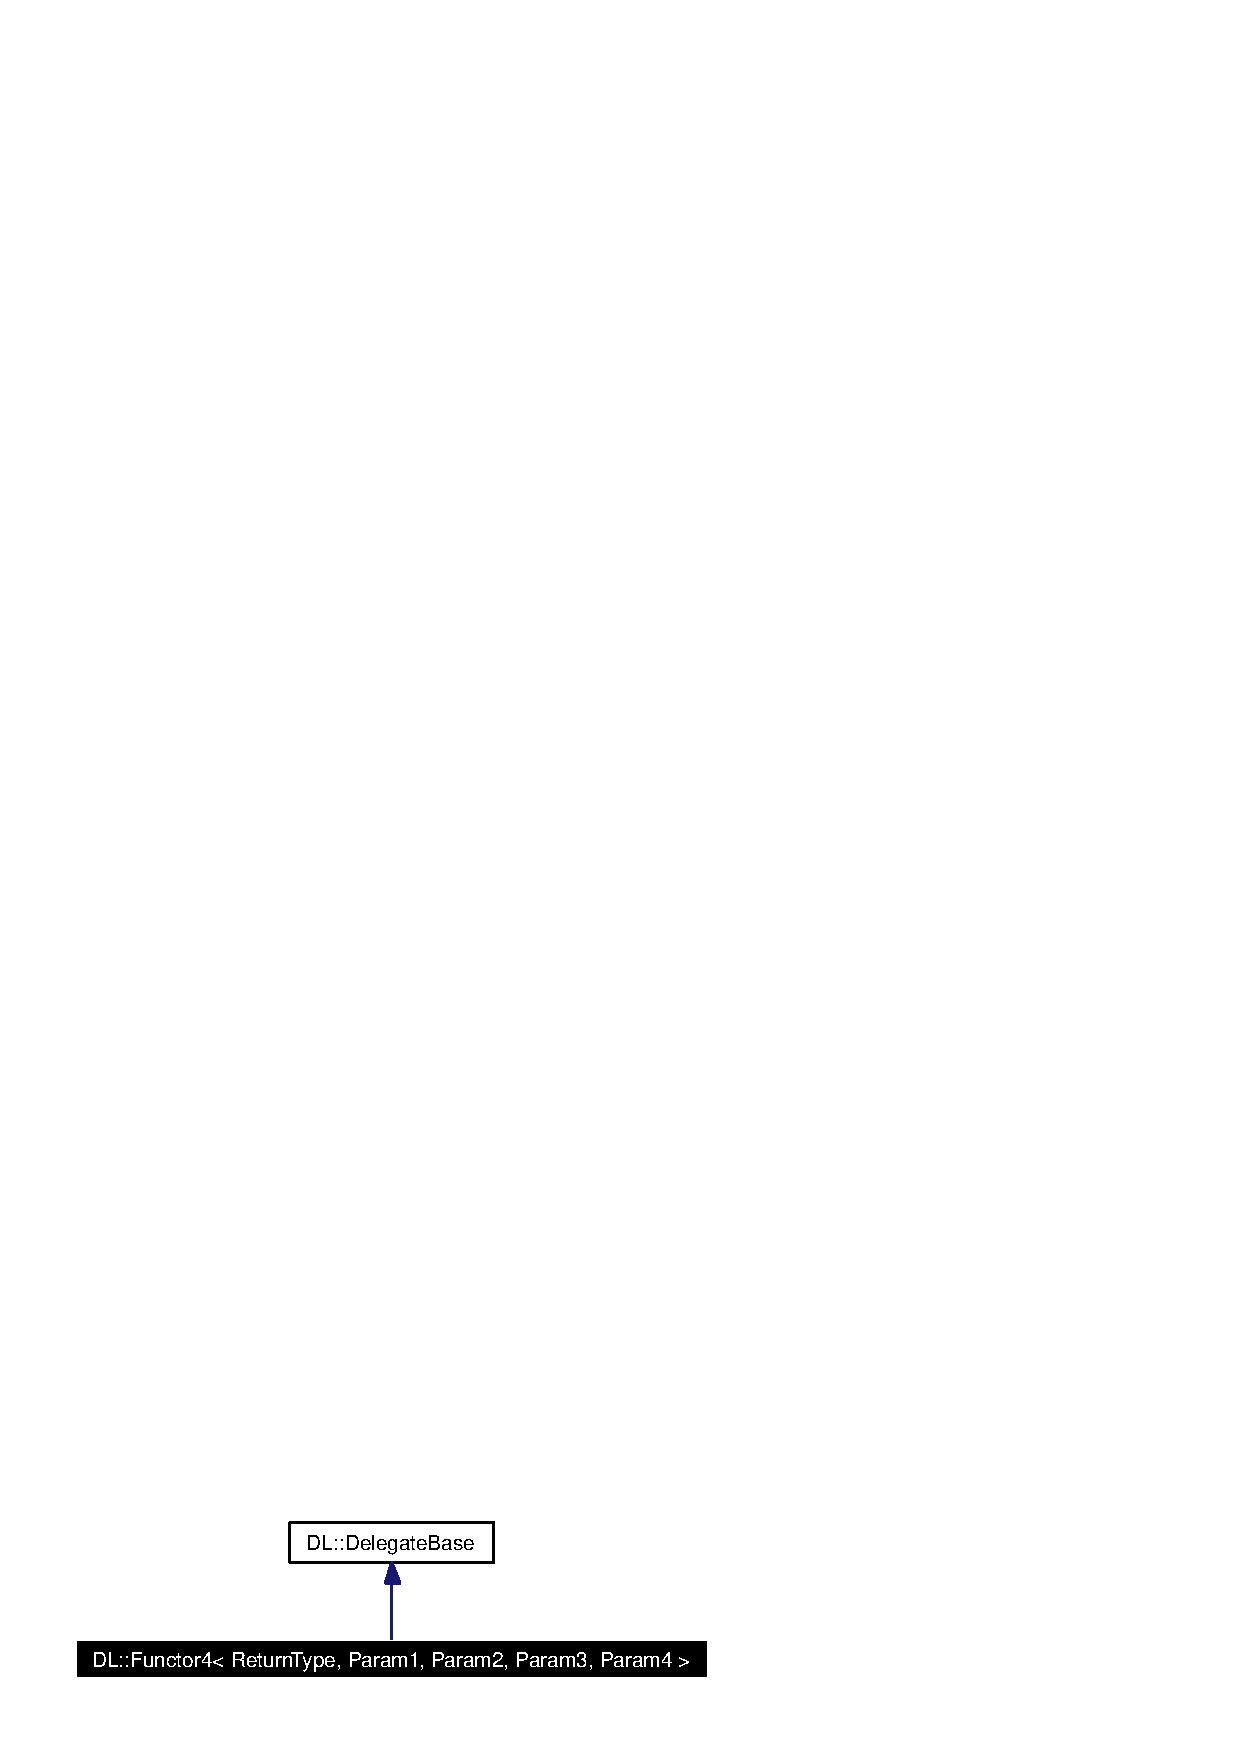
\includegraphics[width=170pt]{classDL_1_1Functor4__inherit__graph}
\end{center}
\end{figure}
Collaboration diagram for DL::Functor4$<$ Return\-Type, Param1, Param2, Param3, Param4 $>$:\begin{figure}[H]
\begin{center}
\leavevmode
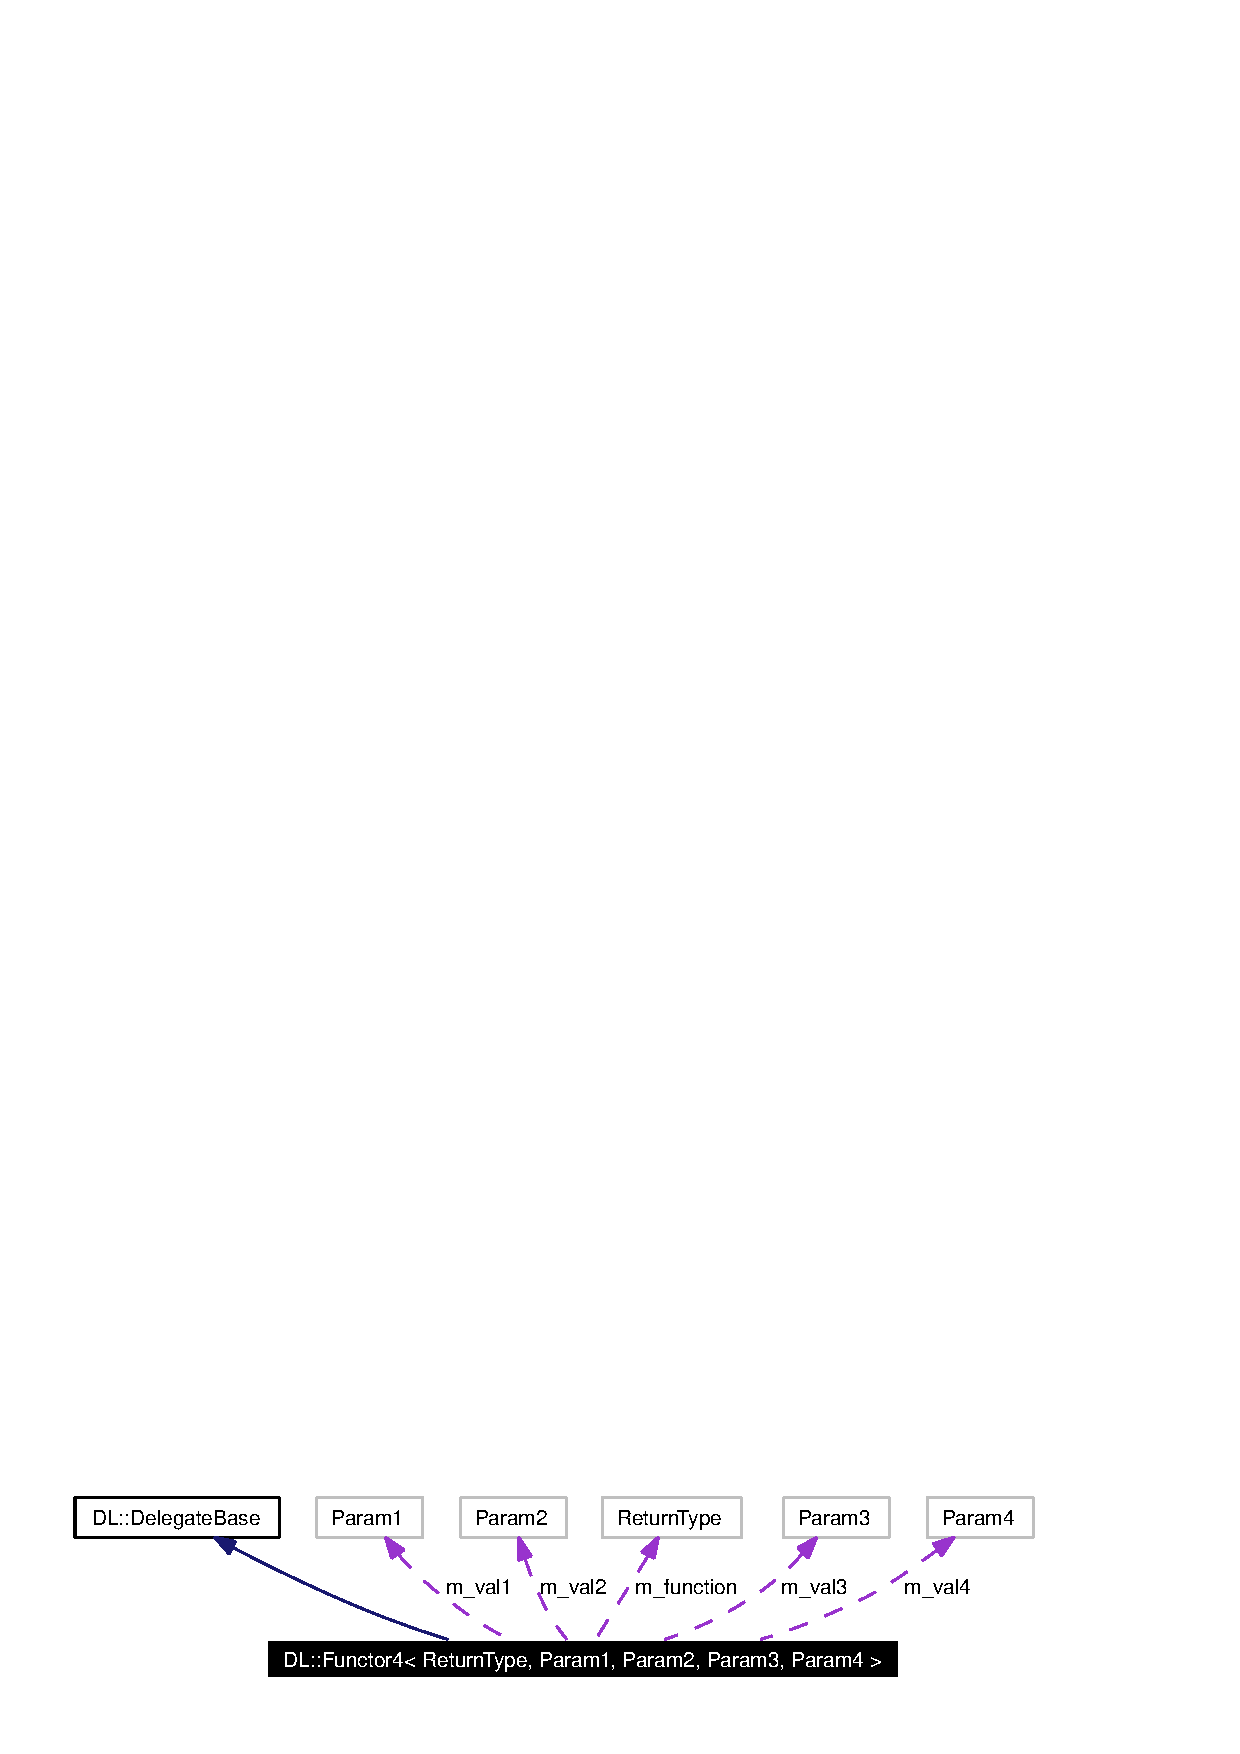
\includegraphics[width=252pt]{classDL_1_1Functor4__coll__graph}
\end{center}
\end{figure}
\subsection*{Public Member Functions}
\begin{CompactItemize}
\item 
\hyperlink{classDL_1_1Functor4_a0}{Functor4} (Return\-Type($\ast$function)(Param1, Param2, Param3, Param4), Param1 val1=Param1(), Param2 val2=Param2(), Param3 val3=Param3(), Param4 val4=Param4())
\item 
virtual \hyperlink{classDL_1_1Functor4_a1}{$\sim$Functor4} ()
\item 
void \hyperlink{classDL_1_1Functor4_a2}{Invoke} ()
\item 
Return\-Type \hyperlink{classDL_1_1Functor4_a3}{Invoke} (Param1 val1, Param2 val2, Param3 val3, Param4 val4)
\end{CompactItemize}
\subsection*{Private Member Functions}
\begin{CompactItemize}
\item 
\hyperlink{classDL_1_1Functor4_d0}{Functor4} ()
\end{CompactItemize}
\subsection*{Private Attributes}
\begin{CompactItemize}
\item 
Return\-Type($\ast$ \hyperlink{classDL_1_1Functor4_r0}{m\_\-function} )(Param1, Param2, Param3, Param4)
\item 
Param1 \hyperlink{classDL_1_1Functor4_r1}{m\_\-val1}
\item 
Param2 \hyperlink{classDL_1_1Functor4_r2}{m\_\-val2}
\item 
Param3 \hyperlink{classDL_1_1Functor4_r3}{m\_\-val3}
\item 
Param4 \hyperlink{classDL_1_1Functor4_r4}{m\_\-val4}
\end{CompactItemize}


\subsection{Detailed Description}
\subsubsection*{template$<$class Return\-Type, class Param1, class Param2, class Param3, class Param4$>$ class DL::Functor4$<$ Return\-Type, Param1, Param2, Param3, Param4 $>$}

Functor for 6 Param



Definition at line 34 of file Functor4.hpp.

\subsection{Constructor \& Destructor Documentation}
\hypertarget{classDL_1_1Functor4_d0}{
\index{DL::Functor4@{DL::Functor4}!Functor4@{Functor4}}
\index{Functor4@{Functor4}!DL::Functor4@{DL::Functor4}}
\subsubsection[Functor4]{\setlength{\rightskip}{0pt plus 5cm}template$<$class Return\-Type, class Param1, class Param2, class Param3, class Param4$>$ \hyperlink{classDL_1_1Functor4}{DL::Functor4}$<$ Return\-Type, Param1, Param2, Param3, Param4 $>$::\hyperlink{classDL_1_1Functor4}{Functor4} ()\hspace{0.3cm}{\tt  \mbox{[}inline, private\mbox{]}}}}
\label{classDL_1_1Functor4_d0}




Definition at line 41 of file Functor4.hpp.\hypertarget{classDL_1_1Functor4_a0}{
\index{DL::Functor4@{DL::Functor4}!Functor4@{Functor4}}
\index{Functor4@{Functor4}!DL::Functor4@{DL::Functor4}}
\subsubsection[Functor4]{\setlength{\rightskip}{0pt plus 5cm}template$<$class Return\-Type, class Param1, class Param2, class Param3, class Param4$>$ \hyperlink{classDL_1_1Functor4}{DL::Functor4}$<$ Return\-Type, Param1, Param2, Param3, Param4 $>$::\hyperlink{classDL_1_1Functor4}{Functor4} (Return\-Type($\ast$)(Param1, Param2, Param3, Param4) {\em function}, Param1 {\em val1} = {\tt Param1()}, Param2 {\em val2} = {\tt Param2()}, Param3 {\em val3} = {\tt Param3()}, Param4 {\em val4} = {\tt Param4()})\hspace{0.3cm}{\tt  \mbox{[}inline\mbox{]}}}}
\label{classDL_1_1Functor4_a0}




Definition at line 43 of file Functor4.hpp.

References DL::Functor4$<$ Return\-Type, Param1, Param2, Param3, Param4 $>$::m\_\-function, DL::Functor4$<$ Return\-Type, Param1, Param2, Param3, Param4 $>$::m\_\-val1, DL::Functor4$<$ Return\-Type, Param1, Param2, Param3, Param4 $>$::m\_\-val2, DL::Functor4$<$ Return\-Type, Param1, Param2, Param3, Param4 $>$::m\_\-val3, and DL::Functor4$<$ Return\-Type, Param1, Param2, Param3, Param4 $>$::m\_\-val4.\hypertarget{classDL_1_1Functor4_a1}{
\index{DL::Functor4@{DL::Functor4}!~Functor4@{$\sim$Functor4}}
\index{~Functor4@{$\sim$Functor4}!DL::Functor4@{DL::Functor4}}
\subsubsection[$\sim$Functor4]{\setlength{\rightskip}{0pt plus 5cm}template$<$class Return\-Type, class Param1, class Param2, class Param3, class Param4$>$ virtual \hyperlink{classDL_1_1Functor4}{DL::Functor4}$<$ Return\-Type, Param1, Param2, Param3, Param4 $>$::$\sim$\hyperlink{classDL_1_1Functor4}{Functor4} ()\hspace{0.3cm}{\tt  \mbox{[}inline, virtual\mbox{]}}}}
\label{classDL_1_1Functor4_a1}




Definition at line 51 of file Functor4.hpp.

\subsection{Member Function Documentation}
\hypertarget{classDL_1_1Functor4_a3}{
\index{DL::Functor4@{DL::Functor4}!Invoke@{Invoke}}
\index{Invoke@{Invoke}!DL::Functor4@{DL::Functor4}}
\subsubsection[Invoke]{\setlength{\rightskip}{0pt plus 5cm}template$<$class Return\-Type, class Param1, class Param2, class Param3, class Param4$>$ Return\-Type \hyperlink{classDL_1_1Functor4}{DL::Functor4}$<$ Return\-Type, Param1, Param2, Param3, Param4 $>$::Invoke (Param1 {\em val1}, Param2 {\em val2}, Param3 {\em val3}, Param4 {\em val4})\hspace{0.3cm}{\tt  \mbox{[}inline\mbox{]}}}}
\label{classDL_1_1Functor4_a3}




Definition at line 56 of file Functor4.hpp.

References DL::Functor4$<$ Return\-Type, Param1, Param2, Param3, Param4 $>$::m\_\-function.\hypertarget{classDL_1_1Functor4_a2}{
\index{DL::Functor4@{DL::Functor4}!Invoke@{Invoke}}
\index{Invoke@{Invoke}!DL::Functor4@{DL::Functor4}}
\subsubsection[Invoke]{\setlength{\rightskip}{0pt plus 5cm}template$<$class Return\-Type, class Param1, class Param2, class Param3, class Param4$>$ void \hyperlink{classDL_1_1Functor4}{DL::Functor4}$<$ Return\-Type, Param1, Param2, Param3, Param4 $>$::Invoke ()\hspace{0.3cm}{\tt  \mbox{[}inline, virtual\mbox{]}}}}
\label{classDL_1_1Functor4_a2}




Implements \hyperlink{classDL_1_1DelegateBase_a2}{DL::Delegate\-Base}.

Definition at line 52 of file Functor4.hpp.

References DL::Functor4$<$ Return\-Type, Param1, Param2, Param3, Param4 $>$::m\_\-val1, DL::Functor4$<$ Return\-Type, Param1, Param2, Param3, Param4 $>$::m\_\-val2, DL::Functor4$<$ Return\-Type, Param1, Param2, Param3, Param4 $>$::m\_\-val3, and DL::Functor4$<$ Return\-Type, Param1, Param2, Param3, Param4 $>$::m\_\-val4.

\subsection{Member Data Documentation}
\hypertarget{classDL_1_1Functor4_r0}{
\index{DL::Functor4@{DL::Functor4}!m_function@{m\_\-function}}
\index{m_function@{m\_\-function}!DL::Functor4@{DL::Functor4}}
\subsubsection[m\_\-function]{\setlength{\rightskip}{0pt plus 5cm}template$<$class Return\-Type, class Param1, class Param2, class Param3, class Param4$>$ Return\-Type($\ast$ \hyperlink{classDL_1_1Functor4}{DL::Functor4}$<$ Return\-Type, Param1, Param2, Param3, Param4 $>$::\hyperlink{classDL_1_1Functor4_r0}{m\_\-function})(Param1, Param2, Param3, Param4)\hspace{0.3cm}{\tt  \mbox{[}private\mbox{]}}}}
\label{classDL_1_1Functor4_r0}




Referenced by DL::Functor4$<$ Return\-Type, Param1, Param2, Param3, Param4 $>$::Functor4(), and DL::Functor4$<$ Return\-Type, Param1, Param2, Param3, Param4 $>$::Invoke().\hypertarget{classDL_1_1Functor4_r1}{
\index{DL::Functor4@{DL::Functor4}!m_val1@{m\_\-val1}}
\index{m_val1@{m\_\-val1}!DL::Functor4@{DL::Functor4}}
\subsubsection[m\_\-val1]{\setlength{\rightskip}{0pt plus 5cm}template$<$class Return\-Type, class Param1, class Param2, class Param3, class Param4$>$ Param1 \hyperlink{classDL_1_1Functor4}{DL::Functor4}$<$ Return\-Type, Param1, Param2, Param3, Param4 $>$::\hyperlink{classDL_1_1Functor4_r1}{m\_\-val1}\hspace{0.3cm}{\tt  \mbox{[}private\mbox{]}}}}
\label{classDL_1_1Functor4_r1}




Definition at line 37 of file Functor4.hpp.

Referenced by DL::Functor4$<$ Return\-Type, Param1, Param2, Param3, Param4 $>$::Functor4(), and DL::Functor4$<$ Return\-Type, Param1, Param2, Param3, Param4 $>$::Invoke().\hypertarget{classDL_1_1Functor4_r2}{
\index{DL::Functor4@{DL::Functor4}!m_val2@{m\_\-val2}}
\index{m_val2@{m\_\-val2}!DL::Functor4@{DL::Functor4}}
\subsubsection[m\_\-val2]{\setlength{\rightskip}{0pt plus 5cm}template$<$class Return\-Type, class Param1, class Param2, class Param3, class Param4$>$ Param2 \hyperlink{classDL_1_1Functor4}{DL::Functor4}$<$ Return\-Type, Param1, Param2, Param3, Param4 $>$::\hyperlink{classDL_1_1Functor4_r2}{m\_\-val2}\hspace{0.3cm}{\tt  \mbox{[}private\mbox{]}}}}
\label{classDL_1_1Functor4_r2}




Definition at line 38 of file Functor4.hpp.

Referenced by DL::Functor4$<$ Return\-Type, Param1, Param2, Param3, Param4 $>$::Functor4(), and DL::Functor4$<$ Return\-Type, Param1, Param2, Param3, Param4 $>$::Invoke().\hypertarget{classDL_1_1Functor4_r3}{
\index{DL::Functor4@{DL::Functor4}!m_val3@{m\_\-val3}}
\index{m_val3@{m\_\-val3}!DL::Functor4@{DL::Functor4}}
\subsubsection[m\_\-val3]{\setlength{\rightskip}{0pt plus 5cm}template$<$class Return\-Type, class Param1, class Param2, class Param3, class Param4$>$ Param3 \hyperlink{classDL_1_1Functor4}{DL::Functor4}$<$ Return\-Type, Param1, Param2, Param3, Param4 $>$::\hyperlink{classDL_1_1Functor4_r3}{m\_\-val3}\hspace{0.3cm}{\tt  \mbox{[}private\mbox{]}}}}
\label{classDL_1_1Functor4_r3}




Definition at line 39 of file Functor4.hpp.

Referenced by DL::Functor4$<$ Return\-Type, Param1, Param2, Param3, Param4 $>$::Functor4(), and DL::Functor4$<$ Return\-Type, Param1, Param2, Param3, Param4 $>$::Invoke().\hypertarget{classDL_1_1Functor4_r4}{
\index{DL::Functor4@{DL::Functor4}!m_val4@{m\_\-val4}}
\index{m_val4@{m\_\-val4}!DL::Functor4@{DL::Functor4}}
\subsubsection[m\_\-val4]{\setlength{\rightskip}{0pt plus 5cm}template$<$class Return\-Type, class Param1, class Param2, class Param3, class Param4$>$ Param4 \hyperlink{classDL_1_1Functor4}{DL::Functor4}$<$ Return\-Type, Param1, Param2, Param3, Param4 $>$::\hyperlink{classDL_1_1Functor4_r4}{m\_\-val4}\hspace{0.3cm}{\tt  \mbox{[}private\mbox{]}}}}
\label{classDL_1_1Functor4_r4}




Definition at line 40 of file Functor4.hpp.

Referenced by DL::Functor4$<$ Return\-Type, Param1, Param2, Param3, Param4 $>$::Functor4(), and DL::Functor4$<$ Return\-Type, Param1, Param2, Param3, Param4 $>$::Invoke().

The documentation for this class was generated from the following file:\begin{CompactItemize}
\item 
/data/callbackext/Functor\-N/\hyperlink{Functor4_8hpp}{Functor4.hpp}\end{CompactItemize}

\hypertarget{classDL_1_1Functor5}{
\section{DL::Functor5$<$ Return\-Type, Param1, Param2, Param3, Param4, Param5 $>$ Class Template Reference}
\label{classDL_1_1Functor5}\index{DL::Functor5@{DL::Functor5}}
}
{\tt \#include $<$Functor5.hpp$>$}

Inherits \hyperlink{classDL_1_1DelegateBase}{DL::Delegate\-Base}.

Inheritance diagram for DL::Functor5$<$ Return\-Type, Param1, Param2, Param3, Param4, Param5 $>$:\begin{figure}[H]
\begin{center}
\leavevmode
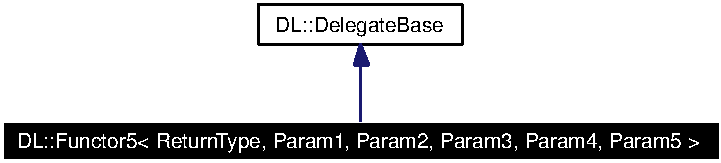
\includegraphics[width=190pt]{classDL_1_1Functor5__inherit__graph}
\end{center}
\end{figure}
Collaboration diagram for DL::Functor5$<$ Return\-Type, Param1, Param2, Param3, Param4, Param5 $>$:\begin{figure}[H]
\begin{center}
\leavevmode
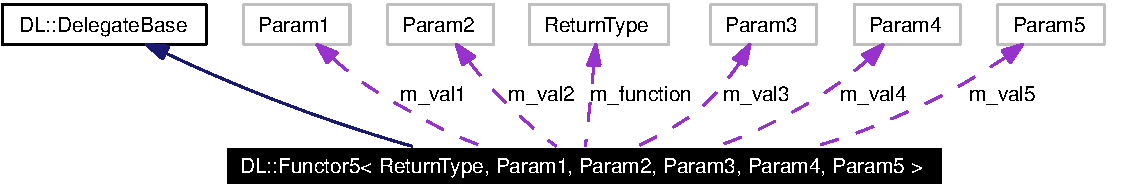
\includegraphics[width=286pt]{classDL_1_1Functor5__coll__graph}
\end{center}
\end{figure}
\subsection*{Public Member Functions}
\begin{CompactItemize}
\item 
\hyperlink{classDL_1_1Functor5_a0}{Functor5} (Return\-Type($\ast$function)(Param1, Param2, Param3, Param4, Param5), Param1 val1=Param1(), Param2 val2=Param2(), Param3 val3=Param3(), Param4 val4=Param4(), Param5 val5=Param5())
\item 
virtual \hyperlink{classDL_1_1Functor5_a1}{$\sim$Functor5} ()
\item 
void \hyperlink{classDL_1_1Functor5_a2}{Invoke} ()
\item 
Return\-Type \hyperlink{classDL_1_1Functor5_a3}{Invoke} (Param1 val1, Param2 val2, Param3 val3, Param4 val4, Param5 val5)
\end{CompactItemize}
\subsection*{Private Member Functions}
\begin{CompactItemize}
\item 
\hyperlink{classDL_1_1Functor5_d0}{Functor5} ()
\end{CompactItemize}
\subsection*{Private Attributes}
\begin{CompactItemize}
\item 
Return\-Type($\ast$ \hyperlink{classDL_1_1Functor5_r0}{m\_\-function} )(Param1, Param2, Param3, Param4, Param5)
\item 
Param1 \hyperlink{classDL_1_1Functor5_r1}{m\_\-val1}
\item 
Param2 \hyperlink{classDL_1_1Functor5_r2}{m\_\-val2}
\item 
Param3 \hyperlink{classDL_1_1Functor5_r3}{m\_\-val3}
\item 
Param4 \hyperlink{classDL_1_1Functor5_r4}{m\_\-val4}
\item 
Param5 \hyperlink{classDL_1_1Functor5_r5}{m\_\-val5}
\end{CompactItemize}


\subsection{Detailed Description}
\subsubsection*{template$<$class Return\-Type, class Param1, class Param2, class Param3, class Param4, class Param5$>$ class DL::Functor5$<$ Return\-Type, Param1, Param2, Param3, Param4, Param5 $>$}

Functor for 6 Param



Definition at line 35 of file Functor5.hpp.

\subsection{Constructor \& Destructor Documentation}
\hypertarget{classDL_1_1Functor5_d0}{
\index{DL::Functor5@{DL::Functor5}!Functor5@{Functor5}}
\index{Functor5@{Functor5}!DL::Functor5@{DL::Functor5}}
\subsubsection[Functor5]{\setlength{\rightskip}{0pt plus 5cm}template$<$class Return\-Type, class Param1, class Param2, class Param3, class Param4, class Param5$>$ \hyperlink{classDL_1_1Functor5}{DL::Functor5}$<$ Return\-Type, Param1, Param2, Param3, Param4, Param5 $>$::\hyperlink{classDL_1_1Functor5}{Functor5} ()\hspace{0.3cm}{\tt  \mbox{[}inline, private\mbox{]}}}}
\label{classDL_1_1Functor5_d0}




Definition at line 43 of file Functor5.hpp.\hypertarget{classDL_1_1Functor5_a0}{
\index{DL::Functor5@{DL::Functor5}!Functor5@{Functor5}}
\index{Functor5@{Functor5}!DL::Functor5@{DL::Functor5}}
\subsubsection[Functor5]{\setlength{\rightskip}{0pt plus 5cm}template$<$class Return\-Type, class Param1, class Param2, class Param3, class Param4, class Param5$>$ \hyperlink{classDL_1_1Functor5}{DL::Functor5}$<$ Return\-Type, Param1, Param2, Param3, Param4, Param5 $>$::\hyperlink{classDL_1_1Functor5}{Functor5} (Return\-Type($\ast$)(Param1, Param2, Param3, Param4, Param5) {\em function}, Param1 {\em val1} = {\tt Param1()}, Param2 {\em val2} = {\tt Param2()}, Param3 {\em val3} = {\tt Param3()}, Param4 {\em val4} = {\tt Param4()}, Param5 {\em val5} = {\tt Param5()})\hspace{0.3cm}{\tt  \mbox{[}inline\mbox{]}}}}
\label{classDL_1_1Functor5_a0}




Definition at line 45 of file Functor5.hpp.

References DL::Functor5$<$ Return\-Type, Param1, Param2, Param3, Param4, Param5 $>$::m\_\-function, DL::Functor5$<$ Return\-Type, Param1, Param2, Param3, Param4, Param5 $>$::m\_\-val1, DL::Functor5$<$ Return\-Type, Param1, Param2, Param3, Param4, Param5 $>$::m\_\-val2, DL::Functor5$<$ Return\-Type, Param1, Param2, Param3, Param4, Param5 $>$::m\_\-val3, DL::Functor5$<$ Return\-Type, Param1, Param2, Param3, Param4, Param5 $>$::m\_\-val4, and DL::Functor5$<$ Return\-Type, Param1, Param2, Param3, Param4, Param5 $>$::m\_\-val5.\hypertarget{classDL_1_1Functor5_a1}{
\index{DL::Functor5@{DL::Functor5}!~Functor5@{$\sim$Functor5}}
\index{~Functor5@{$\sim$Functor5}!DL::Functor5@{DL::Functor5}}
\subsubsection[$\sim$Functor5]{\setlength{\rightskip}{0pt plus 5cm}template$<$class Return\-Type, class Param1, class Param2, class Param3, class Param4, class Param5$>$ virtual \hyperlink{classDL_1_1Functor5}{DL::Functor5}$<$ Return\-Type, Param1, Param2, Param3, Param4, Param5 $>$::$\sim$\hyperlink{classDL_1_1Functor5}{Functor5} ()\hspace{0.3cm}{\tt  \mbox{[}inline, virtual\mbox{]}}}}
\label{classDL_1_1Functor5_a1}




Definition at line 55 of file Functor5.hpp.

\subsection{Member Function Documentation}
\hypertarget{classDL_1_1Functor5_a3}{
\index{DL::Functor5@{DL::Functor5}!Invoke@{Invoke}}
\index{Invoke@{Invoke}!DL::Functor5@{DL::Functor5}}
\subsubsection[Invoke]{\setlength{\rightskip}{0pt plus 5cm}template$<$class Return\-Type, class Param1, class Param2, class Param3, class Param4, class Param5$>$ Return\-Type \hyperlink{classDL_1_1Functor5}{DL::Functor5}$<$ Return\-Type, Param1, Param2, Param3, Param4, Param5 $>$::Invoke (Param1 {\em val1}, Param2 {\em val2}, Param3 {\em val3}, Param4 {\em val4}, Param5 {\em val5})\hspace{0.3cm}{\tt  \mbox{[}inline\mbox{]}}}}
\label{classDL_1_1Functor5_a3}




Definition at line 60 of file Functor5.hpp.

References DL::Functor5$<$ Return\-Type, Param1, Param2, Param3, Param4, Param5 $>$::m\_\-function.\hypertarget{classDL_1_1Functor5_a2}{
\index{DL::Functor5@{DL::Functor5}!Invoke@{Invoke}}
\index{Invoke@{Invoke}!DL::Functor5@{DL::Functor5}}
\subsubsection[Invoke]{\setlength{\rightskip}{0pt plus 5cm}template$<$class Return\-Type, class Param1, class Param2, class Param3, class Param4, class Param5$>$ void \hyperlink{classDL_1_1Functor5}{DL::Functor5}$<$ Return\-Type, Param1, Param2, Param3, Param4, Param5 $>$::Invoke ()\hspace{0.3cm}{\tt  \mbox{[}inline, virtual\mbox{]}}}}
\label{classDL_1_1Functor5_a2}




Implements \hyperlink{classDL_1_1DelegateBase_a2}{DL::Delegate\-Base}.

Definition at line 56 of file Functor5.hpp.

References DL::Functor5$<$ Return\-Type, Param1, Param2, Param3, Param4, Param5 $>$::m\_\-val1, DL::Functor5$<$ Return\-Type, Param1, Param2, Param3, Param4, Param5 $>$::m\_\-val2, DL::Functor5$<$ Return\-Type, Param1, Param2, Param3, Param4, Param5 $>$::m\_\-val3, DL::Functor5$<$ Return\-Type, Param1, Param2, Param3, Param4, Param5 $>$::m\_\-val4, and DL::Functor5$<$ Return\-Type, Param1, Param2, Param3, Param4, Param5 $>$::m\_\-val5.

\subsection{Member Data Documentation}
\hypertarget{classDL_1_1Functor5_r0}{
\index{DL::Functor5@{DL::Functor5}!m_function@{m\_\-function}}
\index{m_function@{m\_\-function}!DL::Functor5@{DL::Functor5}}
\subsubsection[m\_\-function]{\setlength{\rightskip}{0pt plus 5cm}template$<$class Return\-Type, class Param1, class Param2, class Param3, class Param4, class Param5$>$ Return\-Type($\ast$ \hyperlink{classDL_1_1Functor5}{DL::Functor5}$<$ Return\-Type, Param1, Param2, Param3, Param4, Param5 $>$::\hyperlink{classDL_1_1Functor5_r0}{m\_\-function})(Param1, Param2, Param3, Param4, Param5)\hspace{0.3cm}{\tt  \mbox{[}private\mbox{]}}}}
\label{classDL_1_1Functor5_r0}




Referenced by DL::Functor5$<$ Return\-Type, Param1, Param2, Param3, Param4, Param5 $>$::Functor5(), and DL::Functor5$<$ Return\-Type, Param1, Param2, Param3, Param4, Param5 $>$::Invoke().\hypertarget{classDL_1_1Functor5_r1}{
\index{DL::Functor5@{DL::Functor5}!m_val1@{m\_\-val1}}
\index{m_val1@{m\_\-val1}!DL::Functor5@{DL::Functor5}}
\subsubsection[m\_\-val1]{\setlength{\rightskip}{0pt plus 5cm}template$<$class Return\-Type, class Param1, class Param2, class Param3, class Param4, class Param5$>$ Param1 \hyperlink{classDL_1_1Functor5}{DL::Functor5}$<$ Return\-Type, Param1, Param2, Param3, Param4, Param5 $>$::\hyperlink{classDL_1_1Functor5_r1}{m\_\-val1}\hspace{0.3cm}{\tt  \mbox{[}private\mbox{]}}}}
\label{classDL_1_1Functor5_r1}




Definition at line 38 of file Functor5.hpp.

Referenced by DL::Functor5$<$ Return\-Type, Param1, Param2, Param3, Param4, Param5 $>$::Functor5(), and DL::Functor5$<$ Return\-Type, Param1, Param2, Param3, Param4, Param5 $>$::Invoke().\hypertarget{classDL_1_1Functor5_r2}{
\index{DL::Functor5@{DL::Functor5}!m_val2@{m\_\-val2}}
\index{m_val2@{m\_\-val2}!DL::Functor5@{DL::Functor5}}
\subsubsection[m\_\-val2]{\setlength{\rightskip}{0pt plus 5cm}template$<$class Return\-Type, class Param1, class Param2, class Param3, class Param4, class Param5$>$ Param2 \hyperlink{classDL_1_1Functor5}{DL::Functor5}$<$ Return\-Type, Param1, Param2, Param3, Param4, Param5 $>$::\hyperlink{classDL_1_1Functor5_r2}{m\_\-val2}\hspace{0.3cm}{\tt  \mbox{[}private\mbox{]}}}}
\label{classDL_1_1Functor5_r2}




Definition at line 39 of file Functor5.hpp.

Referenced by DL::Functor5$<$ Return\-Type, Param1, Param2, Param3, Param4, Param5 $>$::Functor5(), and DL::Functor5$<$ Return\-Type, Param1, Param2, Param3, Param4, Param5 $>$::Invoke().\hypertarget{classDL_1_1Functor5_r3}{
\index{DL::Functor5@{DL::Functor5}!m_val3@{m\_\-val3}}
\index{m_val3@{m\_\-val3}!DL::Functor5@{DL::Functor5}}
\subsubsection[m\_\-val3]{\setlength{\rightskip}{0pt plus 5cm}template$<$class Return\-Type, class Param1, class Param2, class Param3, class Param4, class Param5$>$ Param3 \hyperlink{classDL_1_1Functor5}{DL::Functor5}$<$ Return\-Type, Param1, Param2, Param3, Param4, Param5 $>$::\hyperlink{classDL_1_1Functor5_r3}{m\_\-val3}\hspace{0.3cm}{\tt  \mbox{[}private\mbox{]}}}}
\label{classDL_1_1Functor5_r3}




Definition at line 40 of file Functor5.hpp.

Referenced by DL::Functor5$<$ Return\-Type, Param1, Param2, Param3, Param4, Param5 $>$::Functor5(), and DL::Functor5$<$ Return\-Type, Param1, Param2, Param3, Param4, Param5 $>$::Invoke().\hypertarget{classDL_1_1Functor5_r4}{
\index{DL::Functor5@{DL::Functor5}!m_val4@{m\_\-val4}}
\index{m_val4@{m\_\-val4}!DL::Functor5@{DL::Functor5}}
\subsubsection[m\_\-val4]{\setlength{\rightskip}{0pt plus 5cm}template$<$class Return\-Type, class Param1, class Param2, class Param3, class Param4, class Param5$>$ Param4 \hyperlink{classDL_1_1Functor5}{DL::Functor5}$<$ Return\-Type, Param1, Param2, Param3, Param4, Param5 $>$::\hyperlink{classDL_1_1Functor5_r4}{m\_\-val4}\hspace{0.3cm}{\tt  \mbox{[}private\mbox{]}}}}
\label{classDL_1_1Functor5_r4}




Definition at line 41 of file Functor5.hpp.

Referenced by DL::Functor5$<$ Return\-Type, Param1, Param2, Param3, Param4, Param5 $>$::Functor5(), and DL::Functor5$<$ Return\-Type, Param1, Param2, Param3, Param4, Param5 $>$::Invoke().\hypertarget{classDL_1_1Functor5_r5}{
\index{DL::Functor5@{DL::Functor5}!m_val5@{m\_\-val5}}
\index{m_val5@{m\_\-val5}!DL::Functor5@{DL::Functor5}}
\subsubsection[m\_\-val5]{\setlength{\rightskip}{0pt plus 5cm}template$<$class Return\-Type, class Param1, class Param2, class Param3, class Param4, class Param5$>$ Param5 \hyperlink{classDL_1_1Functor5}{DL::Functor5}$<$ Return\-Type, Param1, Param2, Param3, Param4, Param5 $>$::\hyperlink{classDL_1_1Functor5_r5}{m\_\-val5}\hspace{0.3cm}{\tt  \mbox{[}private\mbox{]}}}}
\label{classDL_1_1Functor5_r5}




Definition at line 42 of file Functor5.hpp.

Referenced by DL::Functor5$<$ Return\-Type, Param1, Param2, Param3, Param4, Param5 $>$::Functor5(), and DL::Functor5$<$ Return\-Type, Param1, Param2, Param3, Param4, Param5 $>$::Invoke().

The documentation for this class was generated from the following file:\begin{CompactItemize}
\item 
/data/callbackext/Functor\-N/\hyperlink{Functor5_8hpp}{Functor5.hpp}\end{CompactItemize}

\hypertarget{classDL_1_1Functor6}{
\section{DL::Functor6$<$ Return\-Type, Param1, Param2, Param3, Param4, Param5, Param6 $>$ Class Template Reference}
\label{classDL_1_1Functor6}\index{DL::Functor6@{DL::Functor6}}
}
{\tt \#include $<$Functor6.hpp$>$}

Inherits \hyperlink{classDL_1_1DelegateBase}{DL::Delegate\-Base}.

Inheritance diagram for DL::Functor6$<$ Return\-Type, Param1, Param2, Param3, Param4, Param5, Param6 $>$:\begin{figure}[H]
\begin{center}
\leavevmode
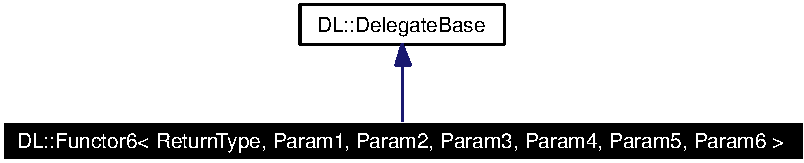
\includegraphics[width=210pt]{classDL_1_1Functor6__inherit__graph}
\end{center}
\end{figure}
Collaboration diagram for DL::Functor6$<$ Return\-Type, Param1, Param2, Param3, Param4, Param5, Param6 $>$:\begin{figure}[H]
\begin{center}
\leavevmode
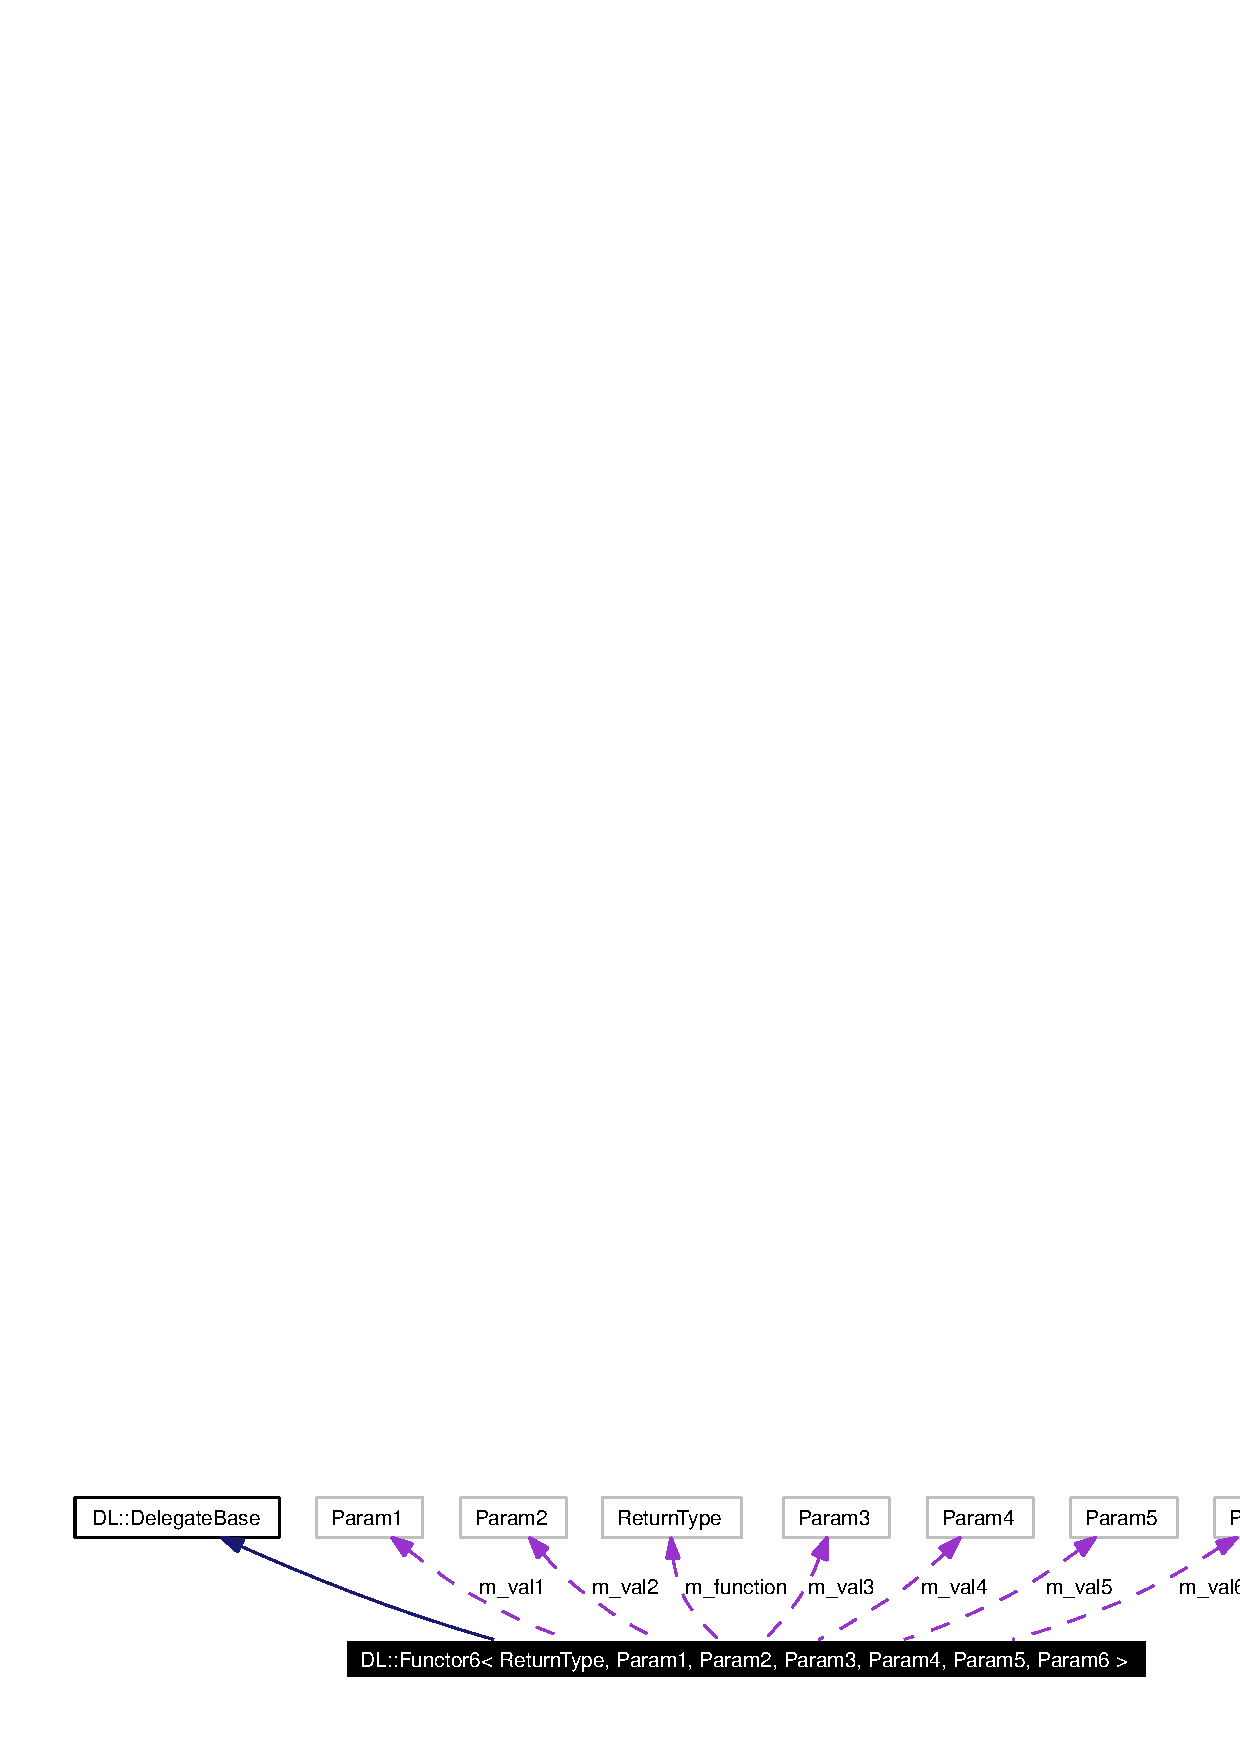
\includegraphics[width=321pt]{classDL_1_1Functor6__coll__graph}
\end{center}
\end{figure}
\subsection*{Public Member Functions}
\begin{CompactItemize}
\item 
\hyperlink{classDL_1_1Functor6_a0}{Functor6} (Return\-Type($\ast$function)(Param1, Param2, Param3, Param4, Param5, Param6), Param1 val1=Param1(), Param2 val2=Param2(), Param3 val3=Param3(), Param4 val4=Param4(), Param5 val5=Param5(), Param6 val6=Param6())
\item 
virtual \hyperlink{classDL_1_1Functor6_a1}{$\sim$Functor6} ()
\item 
void \hyperlink{classDL_1_1Functor6_a2}{Invoke} ()
\item 
Return\-Type \hyperlink{classDL_1_1Functor6_a3}{Invoke} (Param1 val1, Param2 val2, Param3 val3, Param4 val4, Param5 val5, Param6 val6)
\end{CompactItemize}
\subsection*{Private Member Functions}
\begin{CompactItemize}
\item 
\hyperlink{classDL_1_1Functor6_d0}{Functor6} ()
\end{CompactItemize}
\subsection*{Private Attributes}
\begin{CompactItemize}
\item 
Return\-Type($\ast$ \hyperlink{classDL_1_1Functor6_r0}{m\_\-function} )(Param1, Param2, Param3, Param4, Param5, Param6)
\item 
Param1 \hyperlink{classDL_1_1Functor6_r1}{m\_\-val1}
\item 
Param2 \hyperlink{classDL_1_1Functor6_r2}{m\_\-val2}
\item 
Param3 \hyperlink{classDL_1_1Functor6_r3}{m\_\-val3}
\item 
Param4 \hyperlink{classDL_1_1Functor6_r4}{m\_\-val4}
\item 
Param5 \hyperlink{classDL_1_1Functor6_r5}{m\_\-val5}
\item 
Param6 \hyperlink{classDL_1_1Functor6_r6}{m\_\-val6}
\end{CompactItemize}


\subsection{Detailed Description}
\subsubsection*{template$<$class Return\-Type, class Param1, class Param2, class Param3, class Param4, class Param5, class Param6$>$ class DL::Functor6$<$ Return\-Type, Param1, Param2, Param3, Param4, Param5, Param6 $>$}

Functor for 6 Param



Definition at line 36 of file Functor6.hpp.

\subsection{Constructor \& Destructor Documentation}
\hypertarget{classDL_1_1Functor6_d0}{
\index{DL::Functor6@{DL::Functor6}!Functor6@{Functor6}}
\index{Functor6@{Functor6}!DL::Functor6@{DL::Functor6}}
\subsubsection[Functor6]{\setlength{\rightskip}{0pt plus 5cm}template$<$class Return\-Type, class Param1, class Param2, class Param3, class Param4, class Param5, class Param6$>$ \hyperlink{classDL_1_1Functor6}{DL::Functor6}$<$ Return\-Type, Param1, Param2, Param3, Param4, Param5, Param6 $>$::\hyperlink{classDL_1_1Functor6}{Functor6} ()\hspace{0.3cm}{\tt  \mbox{[}inline, private\mbox{]}}}}
\label{classDL_1_1Functor6_d0}




Definition at line 45 of file Functor6.hpp.\hypertarget{classDL_1_1Functor6_a0}{
\index{DL::Functor6@{DL::Functor6}!Functor6@{Functor6}}
\index{Functor6@{Functor6}!DL::Functor6@{DL::Functor6}}
\subsubsection[Functor6]{\setlength{\rightskip}{0pt plus 5cm}template$<$class Return\-Type, class Param1, class Param2, class Param3, class Param4, class Param5, class Param6$>$ \hyperlink{classDL_1_1Functor6}{DL::Functor6}$<$ Return\-Type, Param1, Param2, Param3, Param4, Param5, Param6 $>$::\hyperlink{classDL_1_1Functor6}{Functor6} (Return\-Type($\ast$)(Param1, Param2, Param3, Param4, Param5, Param6) {\em function}, Param1 {\em val1} = {\tt Param1()}, Param2 {\em val2} = {\tt Param2()}, Param3 {\em val3} = {\tt Param3()}, Param4 {\em val4} = {\tt Param4()}, Param5 {\em val5} = {\tt Param5()}, Param6 {\em val6} = {\tt Param6()})\hspace{0.3cm}{\tt  \mbox{[}inline\mbox{]}}}}
\label{classDL_1_1Functor6_a0}




Definition at line 47 of file Functor6.hpp.

References DL::Functor6$<$ Return\-Type, Param1, Param2, Param3, Param4, Param5, Param6 $>$::m\_\-function, DL::Functor6$<$ Return\-Type, Param1, Param2, Param3, Param4, Param5, Param6 $>$::m\_\-val1, DL::Functor6$<$ Return\-Type, Param1, Param2, Param3, Param4, Param5, Param6 $>$::m\_\-val2, DL::Functor6$<$ Return\-Type, Param1, Param2, Param3, Param4, Param5, Param6 $>$::m\_\-val3, DL::Functor6$<$ Return\-Type, Param1, Param2, Param3, Param4, Param5, Param6 $>$::m\_\-val4, DL::Functor6$<$ Return\-Type, Param1, Param2, Param3, Param4, Param5, Param6 $>$::m\_\-val5, and DL::Functor6$<$ Return\-Type, Param1, Param2, Param3, Param4, Param5, Param6 $>$::m\_\-val6.\hypertarget{classDL_1_1Functor6_a1}{
\index{DL::Functor6@{DL::Functor6}!~Functor6@{$\sim$Functor6}}
\index{~Functor6@{$\sim$Functor6}!DL::Functor6@{DL::Functor6}}
\subsubsection[$\sim$Functor6]{\setlength{\rightskip}{0pt plus 5cm}template$<$class Return\-Type, class Param1, class Param2, class Param3, class Param4, class Param5, class Param6$>$ virtual \hyperlink{classDL_1_1Functor6}{DL::Functor6}$<$ Return\-Type, Param1, Param2, Param3, Param4, Param5, Param6 $>$::$\sim$\hyperlink{classDL_1_1Functor6}{Functor6} ()\hspace{0.3cm}{\tt  \mbox{[}inline, virtual\mbox{]}}}}
\label{classDL_1_1Functor6_a1}




Definition at line 58 of file Functor6.hpp.

\subsection{Member Function Documentation}
\hypertarget{classDL_1_1Functor6_a3}{
\index{DL::Functor6@{DL::Functor6}!Invoke@{Invoke}}
\index{Invoke@{Invoke}!DL::Functor6@{DL::Functor6}}
\subsubsection[Invoke]{\setlength{\rightskip}{0pt plus 5cm}template$<$class Return\-Type, class Param1, class Param2, class Param3, class Param4, class Param5, class Param6$>$ Return\-Type \hyperlink{classDL_1_1Functor6}{DL::Functor6}$<$ Return\-Type, Param1, Param2, Param3, Param4, Param5, Param6 $>$::Invoke (Param1 {\em val1}, Param2 {\em val2}, Param3 {\em val3}, Param4 {\em val4}, Param5 {\em val5}, Param6 {\em val6})\hspace{0.3cm}{\tt  \mbox{[}inline\mbox{]}}}}
\label{classDL_1_1Functor6_a3}




Definition at line 63 of file Functor6.hpp.\hypertarget{classDL_1_1Functor6_a2}{
\index{DL::Functor6@{DL::Functor6}!Invoke@{Invoke}}
\index{Invoke@{Invoke}!DL::Functor6@{DL::Functor6}}
\subsubsection[Invoke]{\setlength{\rightskip}{0pt plus 5cm}template$<$class Return\-Type, class Param1, class Param2, class Param3, class Param4, class Param5, class Param6$>$ void \hyperlink{classDL_1_1Functor6}{DL::Functor6}$<$ Return\-Type, Param1, Param2, Param3, Param4, Param5, Param6 $>$::Invoke ()\hspace{0.3cm}{\tt  \mbox{[}inline, virtual\mbox{]}}}}
\label{classDL_1_1Functor6_a2}




Implements \hyperlink{classDL_1_1DelegateBase_a2}{DL::Delegate\-Base}.

Definition at line 59 of file Functor6.hpp.

References DL::Functor6$<$ Return\-Type, Param1, Param2, Param3, Param4, Param5, Param6 $>$::m\_\-val1, DL::Functor6$<$ Return\-Type, Param1, Param2, Param3, Param4, Param5, Param6 $>$::m\_\-val2, DL::Functor6$<$ Return\-Type, Param1, Param2, Param3, Param4, Param5, Param6 $>$::m\_\-val3, DL::Functor6$<$ Return\-Type, Param1, Param2, Param3, Param4, Param5, Param6 $>$::m\_\-val4, DL::Functor6$<$ Return\-Type, Param1, Param2, Param3, Param4, Param5, Param6 $>$::m\_\-val5, and DL::Functor6$<$ Return\-Type, Param1, Param2, Param3, Param4, Param5, Param6 $>$::m\_\-val6.

\subsection{Member Data Documentation}
\hypertarget{classDL_1_1Functor6_r0}{
\index{DL::Functor6@{DL::Functor6}!m_function@{m\_\-function}}
\index{m_function@{m\_\-function}!DL::Functor6@{DL::Functor6}}
\subsubsection[m\_\-function]{\setlength{\rightskip}{0pt plus 5cm}template$<$class Return\-Type, class Param1, class Param2, class Param3, class Param4, class Param5, class Param6$>$ Return\-Type($\ast$ \hyperlink{classDL_1_1Functor6}{DL::Functor6}$<$ Return\-Type, Param1, Param2, Param3, Param4, Param5, Param6 $>$::\hyperlink{classDL_1_1Functor6_r0}{m\_\-function})(Param1, Param2, Param3, Param4, Param5, Param6)\hspace{0.3cm}{\tt  \mbox{[}private\mbox{]}}}}
\label{classDL_1_1Functor6_r0}




Referenced by DL::Functor6$<$ Return\-Type, Param1, Param2, Param3, Param4, Param5, Param6 $>$::Functor6().\hypertarget{classDL_1_1Functor6_r1}{
\index{DL::Functor6@{DL::Functor6}!m_val1@{m\_\-val1}}
\index{m_val1@{m\_\-val1}!DL::Functor6@{DL::Functor6}}
\subsubsection[m\_\-val1]{\setlength{\rightskip}{0pt plus 5cm}template$<$class Return\-Type, class Param1, class Param2, class Param3, class Param4, class Param5, class Param6$>$ Param1 \hyperlink{classDL_1_1Functor6}{DL::Functor6}$<$ Return\-Type, Param1, Param2, Param3, Param4, Param5, Param6 $>$::\hyperlink{classDL_1_1Functor6_r1}{m\_\-val1}\hspace{0.3cm}{\tt  \mbox{[}private\mbox{]}}}}
\label{classDL_1_1Functor6_r1}




Definition at line 39 of file Functor6.hpp.

Referenced by DL::Functor6$<$ Return\-Type, Param1, Param2, Param3, Param4, Param5, Param6 $>$::Functor6(), and DL::Functor6$<$ Return\-Type, Param1, Param2, Param3, Param4, Param5, Param6 $>$::Invoke().\hypertarget{classDL_1_1Functor6_r2}{
\index{DL::Functor6@{DL::Functor6}!m_val2@{m\_\-val2}}
\index{m_val2@{m\_\-val2}!DL::Functor6@{DL::Functor6}}
\subsubsection[m\_\-val2]{\setlength{\rightskip}{0pt plus 5cm}template$<$class Return\-Type, class Param1, class Param2, class Param3, class Param4, class Param5, class Param6$>$ Param2 \hyperlink{classDL_1_1Functor6}{DL::Functor6}$<$ Return\-Type, Param1, Param2, Param3, Param4, Param5, Param6 $>$::\hyperlink{classDL_1_1Functor6_r2}{m\_\-val2}\hspace{0.3cm}{\tt  \mbox{[}private\mbox{]}}}}
\label{classDL_1_1Functor6_r2}




Definition at line 40 of file Functor6.hpp.

Referenced by DL::Functor6$<$ Return\-Type, Param1, Param2, Param3, Param4, Param5, Param6 $>$::Functor6(), and DL::Functor6$<$ Return\-Type, Param1, Param2, Param3, Param4, Param5, Param6 $>$::Invoke().\hypertarget{classDL_1_1Functor6_r3}{
\index{DL::Functor6@{DL::Functor6}!m_val3@{m\_\-val3}}
\index{m_val3@{m\_\-val3}!DL::Functor6@{DL::Functor6}}
\subsubsection[m\_\-val3]{\setlength{\rightskip}{0pt plus 5cm}template$<$class Return\-Type, class Param1, class Param2, class Param3, class Param4, class Param5, class Param6$>$ Param3 \hyperlink{classDL_1_1Functor6}{DL::Functor6}$<$ Return\-Type, Param1, Param2, Param3, Param4, Param5, Param6 $>$::\hyperlink{classDL_1_1Functor6_r3}{m\_\-val3}\hspace{0.3cm}{\tt  \mbox{[}private\mbox{]}}}}
\label{classDL_1_1Functor6_r3}




Definition at line 41 of file Functor6.hpp.

Referenced by DL::Functor6$<$ Return\-Type, Param1, Param2, Param3, Param4, Param5, Param6 $>$::Functor6(), and DL::Functor6$<$ Return\-Type, Param1, Param2, Param3, Param4, Param5, Param6 $>$::Invoke().\hypertarget{classDL_1_1Functor6_r4}{
\index{DL::Functor6@{DL::Functor6}!m_val4@{m\_\-val4}}
\index{m_val4@{m\_\-val4}!DL::Functor6@{DL::Functor6}}
\subsubsection[m\_\-val4]{\setlength{\rightskip}{0pt plus 5cm}template$<$class Return\-Type, class Param1, class Param2, class Param3, class Param4, class Param5, class Param6$>$ Param4 \hyperlink{classDL_1_1Functor6}{DL::Functor6}$<$ Return\-Type, Param1, Param2, Param3, Param4, Param5, Param6 $>$::\hyperlink{classDL_1_1Functor6_r4}{m\_\-val4}\hspace{0.3cm}{\tt  \mbox{[}private\mbox{]}}}}
\label{classDL_1_1Functor6_r4}




Definition at line 42 of file Functor6.hpp.

Referenced by DL::Functor6$<$ Return\-Type, Param1, Param2, Param3, Param4, Param5, Param6 $>$::Functor6(), and DL::Functor6$<$ Return\-Type, Param1, Param2, Param3, Param4, Param5, Param6 $>$::Invoke().\hypertarget{classDL_1_1Functor6_r5}{
\index{DL::Functor6@{DL::Functor6}!m_val5@{m\_\-val5}}
\index{m_val5@{m\_\-val5}!DL::Functor6@{DL::Functor6}}
\subsubsection[m\_\-val5]{\setlength{\rightskip}{0pt plus 5cm}template$<$class Return\-Type, class Param1, class Param2, class Param3, class Param4, class Param5, class Param6$>$ Param5 \hyperlink{classDL_1_1Functor6}{DL::Functor6}$<$ Return\-Type, Param1, Param2, Param3, Param4, Param5, Param6 $>$::\hyperlink{classDL_1_1Functor6_r5}{m\_\-val5}\hspace{0.3cm}{\tt  \mbox{[}private\mbox{]}}}}
\label{classDL_1_1Functor6_r5}




Definition at line 43 of file Functor6.hpp.

Referenced by DL::Functor6$<$ Return\-Type, Param1, Param2, Param3, Param4, Param5, Param6 $>$::Functor6(), and DL::Functor6$<$ Return\-Type, Param1, Param2, Param3, Param4, Param5, Param6 $>$::Invoke().\hypertarget{classDL_1_1Functor6_r6}{
\index{DL::Functor6@{DL::Functor6}!m_val6@{m\_\-val6}}
\index{m_val6@{m\_\-val6}!DL::Functor6@{DL::Functor6}}
\subsubsection[m\_\-val6]{\setlength{\rightskip}{0pt plus 5cm}template$<$class Return\-Type, class Param1, class Param2, class Param3, class Param4, class Param5, class Param6$>$ Param6 \hyperlink{classDL_1_1Functor6}{DL::Functor6}$<$ Return\-Type, Param1, Param2, Param3, Param4, Param5, Param6 $>$::\hyperlink{classDL_1_1Functor6_r6}{m\_\-val6}\hspace{0.3cm}{\tt  \mbox{[}private\mbox{]}}}}
\label{classDL_1_1Functor6_r6}




Definition at line 44 of file Functor6.hpp.

Referenced by DL::Functor6$<$ Return\-Type, Param1, Param2, Param3, Param4, Param5, Param6 $>$::Functor6(), and DL::Functor6$<$ Return\-Type, Param1, Param2, Param3, Param4, Param5, Param6 $>$::Invoke().

The documentation for this class was generated from the following file:\begin{CompactItemize}
\item 
/data/callbackext/Functor\-N/\hyperlink{Functor6_8hpp}{Functor6.hpp}\end{CompactItemize}

\hypertarget{classDL_1_1Functor7}{
\section{DL::Functor7$<$ Return\-Type, Param1, Param2, Param3, Param4, Param5, Param6, Param7 $>$ Class Template Reference}
\label{classDL_1_1Functor7}\index{DL::Functor7@{DL::Functor7}}
}
{\tt \#include $<$Functor7.hpp$>$}

Inherits \hyperlink{classDL_1_1DelegateBase}{DL::Delegate\-Base}.

Inheritance diagram for DL::Functor7$<$ Return\-Type, Param1, Param2, Param3, Param4, Param5, Param6, Param7 $>$:\begin{figure}[H]
\begin{center}
\leavevmode
\includegraphics[width=231pt]{classDL_1_1Functor7__inherit__graph}
\end{center}
\end{figure}
Collaboration diagram for DL::Functor7$<$ Return\-Type, Param1, Param2, Param3, Param4, Param5, Param6, Param7 $>$:\begin{figure}[H]
\begin{center}
\leavevmode
\includegraphics[width=355pt]{classDL_1_1Functor7__coll__graph}
\end{center}
\end{figure}
\subsection*{Public Member Functions}
\begin{CompactItemize}
\item 
\hyperlink{classDL_1_1Functor7_a0}{Functor7} (Return\-Type($\ast$function)(Param1, Param2, Param3, Param4, Param5, Param6, Param7), Param1 val1=Param1(), Param2 val2=Param2(), Param3 val3=Param3(), Param4 val4=Param4(), Param5 val5=Param5(), Param6 val6=Param6(), Param7 val7=Param7())
\item 
virtual \hyperlink{classDL_1_1Functor7_a1}{$\sim$Functor7} ()
\item 
void \hyperlink{classDL_1_1Functor7_a2}{Invoke} ()
\item 
Return\-Type \hyperlink{classDL_1_1Functor7_a3}{Invoke} (Param1 val1, Param2 val2, Param3 val3, Param4 val4, Param5 val5, Param6 val6, Param7 val7)
\end{CompactItemize}
\subsection*{Private Member Functions}
\begin{CompactItemize}
\item 
\hyperlink{classDL_1_1Functor7_d0}{Functor7} ()
\end{CompactItemize}
\subsection*{Private Attributes}
\begin{CompactItemize}
\item 
Return\-Type($\ast$ \hyperlink{classDL_1_1Functor7_r0}{m\_\-function} )(Param1, Param2, Param3, Param4, Param5, Param6, Param7)
\item 
Param1 \hyperlink{classDL_1_1Functor7_r1}{m\_\-val1}
\item 
Param2 \hyperlink{classDL_1_1Functor7_r2}{m\_\-val2}
\item 
Param3 \hyperlink{classDL_1_1Functor7_r3}{m\_\-val3}
\item 
Param4 \hyperlink{classDL_1_1Functor7_r4}{m\_\-val4}
\item 
Param5 \hyperlink{classDL_1_1Functor7_r5}{m\_\-val5}
\item 
Param6 \hyperlink{classDL_1_1Functor7_r6}{m\_\-val6}
\item 
Param7 \hyperlink{classDL_1_1Functor7_r7}{m\_\-val7}
\end{CompactItemize}


\subsection{Detailed Description}
\subsubsection*{template$<$class Return\-Type, class Param1, class Param2, class Param3, class Param4, class Param5, class Param6, class Param7$>$ class DL::Functor7$<$ Return\-Type, Param1, Param2, Param3, Param4, Param5, Param6, Param7 $>$}

Functor for 8 Param



Definition at line 37 of file Functor7.hpp.

\subsection{Constructor \& Destructor Documentation}
\hypertarget{classDL_1_1Functor7_d0}{
\index{DL::Functor7@{DL::Functor7}!Functor7@{Functor7}}
\index{Functor7@{Functor7}!DL::Functor7@{DL::Functor7}}
\subsubsection[Functor7]{\setlength{\rightskip}{0pt plus 5cm}template$<$class Return\-Type, class Param1, class Param2, class Param3, class Param4, class Param5, class Param6, class Param7$>$ \hyperlink{classDL_1_1Functor7}{DL::Functor7}$<$ Return\-Type, Param1, Param2, Param3, Param4, Param5, Param6, Param7 $>$::\hyperlink{classDL_1_1Functor7}{Functor7} ()\hspace{0.3cm}{\tt  \mbox{[}inline, private\mbox{]}}}}
\label{classDL_1_1Functor7_d0}




Definition at line 47 of file Functor7.hpp.\hypertarget{classDL_1_1Functor7_a0}{
\index{DL::Functor7@{DL::Functor7}!Functor7@{Functor7}}
\index{Functor7@{Functor7}!DL::Functor7@{DL::Functor7}}
\subsubsection[Functor7]{\setlength{\rightskip}{0pt plus 5cm}template$<$class Return\-Type, class Param1, class Param2, class Param3, class Param4, class Param5, class Param6, class Param7$>$ \hyperlink{classDL_1_1Functor7}{DL::Functor7}$<$ Return\-Type, Param1, Param2, Param3, Param4, Param5, Param6, Param7 $>$::\hyperlink{classDL_1_1Functor7}{Functor7} (Return\-Type($\ast$)(Param1, Param2, Param3, Param4, Param5, Param6, Param7) {\em function}, Param1 {\em val1} = {\tt Param1()}, Param2 {\em val2} = {\tt Param2()}, Param3 {\em val3} = {\tt Param3()}, Param4 {\em val4} = {\tt Param4()}, Param5 {\em val5} = {\tt Param5()}, Param6 {\em val6} = {\tt Param6()}, Param7 {\em val7} = {\tt Param7()})\hspace{0.3cm}{\tt  \mbox{[}inline\mbox{]}}}}
\label{classDL_1_1Functor7_a0}




Definition at line 49 of file Functor7.hpp.

References DL::Functor7$<$ Return\-Type, Param1, Param2, Param3, Param4, Param5, Param6, Param7 $>$::m\_\-function, DL::Functor7$<$ Return\-Type, Param1, Param2, Param3, Param4, Param5, Param6, Param7 $>$::m\_\-val1, DL::Functor7$<$ Return\-Type, Param1, Param2, Param3, Param4, Param5, Param6, Param7 $>$::m\_\-val2, DL::Functor7$<$ Return\-Type, Param1, Param2, Param3, Param4, Param5, Param6, Param7 $>$::m\_\-val3, DL::Functor7$<$ Return\-Type, Param1, Param2, Param3, Param4, Param5, Param6, Param7 $>$::m\_\-val4, DL::Functor7$<$ Return\-Type, Param1, Param2, Param3, Param4, Param5, Param6, Param7 $>$::m\_\-val5, DL::Functor7$<$ Return\-Type, Param1, Param2, Param3, Param4, Param5, Param6, Param7 $>$::m\_\-val6, and DL::Functor7$<$ Return\-Type, Param1, Param2, Param3, Param4, Param5, Param6, Param7 $>$::m\_\-val7.\hypertarget{classDL_1_1Functor7_a1}{
\index{DL::Functor7@{DL::Functor7}!~Functor7@{$\sim$Functor7}}
\index{~Functor7@{$\sim$Functor7}!DL::Functor7@{DL::Functor7}}
\subsubsection[$\sim$Functor7]{\setlength{\rightskip}{0pt plus 5cm}template$<$class Return\-Type, class Param1, class Param2, class Param3, class Param4, class Param5, class Param6, class Param7$>$ virtual \hyperlink{classDL_1_1Functor7}{DL::Functor7}$<$ Return\-Type, Param1, Param2, Param3, Param4, Param5, Param6, Param7 $>$::$\sim$\hyperlink{classDL_1_1Functor7}{Functor7} ()\hspace{0.3cm}{\tt  \mbox{[}inline, virtual\mbox{]}}}}
\label{classDL_1_1Functor7_a1}




Definition at line 62 of file Functor7.hpp.

\subsection{Member Function Documentation}
\hypertarget{classDL_1_1Functor7_a3}{
\index{DL::Functor7@{DL::Functor7}!Invoke@{Invoke}}
\index{Invoke@{Invoke}!DL::Functor7@{DL::Functor7}}
\subsubsection[Invoke]{\setlength{\rightskip}{0pt plus 5cm}template$<$class Return\-Type, class Param1, class Param2, class Param3, class Param4, class Param5, class Param6, class Param7$>$ Return\-Type \hyperlink{classDL_1_1Functor7}{DL::Functor7}$<$ Return\-Type, Param1, Param2, Param3, Param4, Param5, Param6, Param7 $>$::Invoke (Param1 {\em val1}, Param2 {\em val2}, Param3 {\em val3}, Param4 {\em val4}, Param5 {\em val5}, Param6 {\em val6}, Param7 {\em val7})\hspace{0.3cm}{\tt  \mbox{[}inline\mbox{]}}}}
\label{classDL_1_1Functor7_a3}




Definition at line 67 of file Functor7.hpp.\hypertarget{classDL_1_1Functor7_a2}{
\index{DL::Functor7@{DL::Functor7}!Invoke@{Invoke}}
\index{Invoke@{Invoke}!DL::Functor7@{DL::Functor7}}
\subsubsection[Invoke]{\setlength{\rightskip}{0pt plus 5cm}template$<$class Return\-Type, class Param1, class Param2, class Param3, class Param4, class Param5, class Param6, class Param7$>$ void \hyperlink{classDL_1_1Functor7}{DL::Functor7}$<$ Return\-Type, Param1, Param2, Param3, Param4, Param5, Param6, Param7 $>$::Invoke ()\hspace{0.3cm}{\tt  \mbox{[}inline, virtual\mbox{]}}}}
\label{classDL_1_1Functor7_a2}




Implements \hyperlink{classDL_1_1DelegateBase_a2}{DL::Delegate\-Base}.

Definition at line 63 of file Functor7.hpp.

References DL::Functor7$<$ Return\-Type, Param1, Param2, Param3, Param4, Param5, Param6, Param7 $>$::m\_\-val1, DL::Functor7$<$ Return\-Type, Param1, Param2, Param3, Param4, Param5, Param6, Param7 $>$::m\_\-val2, DL::Functor7$<$ Return\-Type, Param1, Param2, Param3, Param4, Param5, Param6, Param7 $>$::m\_\-val3, DL::Functor7$<$ Return\-Type, Param1, Param2, Param3, Param4, Param5, Param6, Param7 $>$::m\_\-val4, DL::Functor7$<$ Return\-Type, Param1, Param2, Param3, Param4, Param5, Param6, Param7 $>$::m\_\-val5, DL::Functor7$<$ Return\-Type, Param1, Param2, Param3, Param4, Param5, Param6, Param7 $>$::m\_\-val6, and DL::Functor7$<$ Return\-Type, Param1, Param2, Param3, Param4, Param5, Param6, Param7 $>$::m\_\-val7.

\subsection{Member Data Documentation}
\hypertarget{classDL_1_1Functor7_r0}{
\index{DL::Functor7@{DL::Functor7}!m_function@{m\_\-function}}
\index{m_function@{m\_\-function}!DL::Functor7@{DL::Functor7}}
\subsubsection[m\_\-function]{\setlength{\rightskip}{0pt plus 5cm}template$<$class Return\-Type, class Param1, class Param2, class Param3, class Param4, class Param5, class Param6, class Param7$>$ Return\-Type($\ast$ \hyperlink{classDL_1_1Functor7}{DL::Functor7}$<$ Return\-Type, Param1, Param2, Param3, Param4, Param5, Param6, Param7 $>$::\hyperlink{classDL_1_1Functor7_r0}{m\_\-function})(Param1, Param2, Param3, Param4, Param5, Param6, Param7)\hspace{0.3cm}{\tt  \mbox{[}private\mbox{]}}}}
\label{classDL_1_1Functor7_r0}




Referenced by DL::Functor7$<$ Return\-Type, Param1, Param2, Param3, Param4, Param5, Param6, Param7 $>$::Functor7().\hypertarget{classDL_1_1Functor7_r1}{
\index{DL::Functor7@{DL::Functor7}!m_val1@{m\_\-val1}}
\index{m_val1@{m\_\-val1}!DL::Functor7@{DL::Functor7}}
\subsubsection[m\_\-val1]{\setlength{\rightskip}{0pt plus 5cm}template$<$class Return\-Type, class Param1, class Param2, class Param3, class Param4, class Param5, class Param6, class Param7$>$ Param1 \hyperlink{classDL_1_1Functor7}{DL::Functor7}$<$ Return\-Type, Param1, Param2, Param3, Param4, Param5, Param6, Param7 $>$::\hyperlink{classDL_1_1Functor7_r1}{m\_\-val1}\hspace{0.3cm}{\tt  \mbox{[}private\mbox{]}}}}
\label{classDL_1_1Functor7_r1}




Definition at line 40 of file Functor7.hpp.

Referenced by DL::Functor7$<$ Return\-Type, Param1, Param2, Param3, Param4, Param5, Param6, Param7 $>$::Functor7(), and DL::Functor7$<$ Return\-Type, Param1, Param2, Param3, Param4, Param5, Param6, Param7 $>$::Invoke().\hypertarget{classDL_1_1Functor7_r2}{
\index{DL::Functor7@{DL::Functor7}!m_val2@{m\_\-val2}}
\index{m_val2@{m\_\-val2}!DL::Functor7@{DL::Functor7}}
\subsubsection[m\_\-val2]{\setlength{\rightskip}{0pt plus 5cm}template$<$class Return\-Type, class Param1, class Param2, class Param3, class Param4, class Param5, class Param6, class Param7$>$ Param2 \hyperlink{classDL_1_1Functor7}{DL::Functor7}$<$ Return\-Type, Param1, Param2, Param3, Param4, Param5, Param6, Param7 $>$::\hyperlink{classDL_1_1Functor7_r2}{m\_\-val2}\hspace{0.3cm}{\tt  \mbox{[}private\mbox{]}}}}
\label{classDL_1_1Functor7_r2}




Definition at line 41 of file Functor7.hpp.

Referenced by DL::Functor7$<$ Return\-Type, Param1, Param2, Param3, Param4, Param5, Param6, Param7 $>$::Functor7(), and DL::Functor7$<$ Return\-Type, Param1, Param2, Param3, Param4, Param5, Param6, Param7 $>$::Invoke().\hypertarget{classDL_1_1Functor7_r3}{
\index{DL::Functor7@{DL::Functor7}!m_val3@{m\_\-val3}}
\index{m_val3@{m\_\-val3}!DL::Functor7@{DL::Functor7}}
\subsubsection[m\_\-val3]{\setlength{\rightskip}{0pt plus 5cm}template$<$class Return\-Type, class Param1, class Param2, class Param3, class Param4, class Param5, class Param6, class Param7$>$ Param3 \hyperlink{classDL_1_1Functor7}{DL::Functor7}$<$ Return\-Type, Param1, Param2, Param3, Param4, Param5, Param6, Param7 $>$::\hyperlink{classDL_1_1Functor7_r3}{m\_\-val3}\hspace{0.3cm}{\tt  \mbox{[}private\mbox{]}}}}
\label{classDL_1_1Functor7_r3}




Definition at line 42 of file Functor7.hpp.

Referenced by DL::Functor7$<$ Return\-Type, Param1, Param2, Param3, Param4, Param5, Param6, Param7 $>$::Functor7(), and DL::Functor7$<$ Return\-Type, Param1, Param2, Param3, Param4, Param5, Param6, Param7 $>$::Invoke().\hypertarget{classDL_1_1Functor7_r4}{
\index{DL::Functor7@{DL::Functor7}!m_val4@{m\_\-val4}}
\index{m_val4@{m\_\-val4}!DL::Functor7@{DL::Functor7}}
\subsubsection[m\_\-val4]{\setlength{\rightskip}{0pt plus 5cm}template$<$class Return\-Type, class Param1, class Param2, class Param3, class Param4, class Param5, class Param6, class Param7$>$ Param4 \hyperlink{classDL_1_1Functor7}{DL::Functor7}$<$ Return\-Type, Param1, Param2, Param3, Param4, Param5, Param6, Param7 $>$::\hyperlink{classDL_1_1Functor7_r4}{m\_\-val4}\hspace{0.3cm}{\tt  \mbox{[}private\mbox{]}}}}
\label{classDL_1_1Functor7_r4}




Definition at line 43 of file Functor7.hpp.

Referenced by DL::Functor7$<$ Return\-Type, Param1, Param2, Param3, Param4, Param5, Param6, Param7 $>$::Functor7(), and DL::Functor7$<$ Return\-Type, Param1, Param2, Param3, Param4, Param5, Param6, Param7 $>$::Invoke().\hypertarget{classDL_1_1Functor7_r5}{
\index{DL::Functor7@{DL::Functor7}!m_val5@{m\_\-val5}}
\index{m_val5@{m\_\-val5}!DL::Functor7@{DL::Functor7}}
\subsubsection[m\_\-val5]{\setlength{\rightskip}{0pt plus 5cm}template$<$class Return\-Type, class Param1, class Param2, class Param3, class Param4, class Param5, class Param6, class Param7$>$ Param5 \hyperlink{classDL_1_1Functor7}{DL::Functor7}$<$ Return\-Type, Param1, Param2, Param3, Param4, Param5, Param6, Param7 $>$::\hyperlink{classDL_1_1Functor7_r5}{m\_\-val5}\hspace{0.3cm}{\tt  \mbox{[}private\mbox{]}}}}
\label{classDL_1_1Functor7_r5}




Definition at line 44 of file Functor7.hpp.

Referenced by DL::Functor7$<$ Return\-Type, Param1, Param2, Param3, Param4, Param5, Param6, Param7 $>$::Functor7(), and DL::Functor7$<$ Return\-Type, Param1, Param2, Param3, Param4, Param5, Param6, Param7 $>$::Invoke().\hypertarget{classDL_1_1Functor7_r6}{
\index{DL::Functor7@{DL::Functor7}!m_val6@{m\_\-val6}}
\index{m_val6@{m\_\-val6}!DL::Functor7@{DL::Functor7}}
\subsubsection[m\_\-val6]{\setlength{\rightskip}{0pt plus 5cm}template$<$class Return\-Type, class Param1, class Param2, class Param3, class Param4, class Param5, class Param6, class Param7$>$ Param6 \hyperlink{classDL_1_1Functor7}{DL::Functor7}$<$ Return\-Type, Param1, Param2, Param3, Param4, Param5, Param6, Param7 $>$::\hyperlink{classDL_1_1Functor7_r6}{m\_\-val6}\hspace{0.3cm}{\tt  \mbox{[}private\mbox{]}}}}
\label{classDL_1_1Functor7_r6}




Definition at line 45 of file Functor7.hpp.

Referenced by DL::Functor7$<$ Return\-Type, Param1, Param2, Param3, Param4, Param5, Param6, Param7 $>$::Functor7(), and DL::Functor7$<$ Return\-Type, Param1, Param2, Param3, Param4, Param5, Param6, Param7 $>$::Invoke().\hypertarget{classDL_1_1Functor7_r7}{
\index{DL::Functor7@{DL::Functor7}!m_val7@{m\_\-val7}}
\index{m_val7@{m\_\-val7}!DL::Functor7@{DL::Functor7}}
\subsubsection[m\_\-val7]{\setlength{\rightskip}{0pt plus 5cm}template$<$class Return\-Type, class Param1, class Param2, class Param3, class Param4, class Param5, class Param6, class Param7$>$ Param7 \hyperlink{classDL_1_1Functor7}{DL::Functor7}$<$ Return\-Type, Param1, Param2, Param3, Param4, Param5, Param6, Param7 $>$::\hyperlink{classDL_1_1Functor7_r7}{m\_\-val7}\hspace{0.3cm}{\tt  \mbox{[}private\mbox{]}}}}
\label{classDL_1_1Functor7_r7}




Definition at line 46 of file Functor7.hpp.

Referenced by DL::Functor7$<$ Return\-Type, Param1, Param2, Param3, Param4, Param5, Param6, Param7 $>$::Functor7(), and DL::Functor7$<$ Return\-Type, Param1, Param2, Param3, Param4, Param5, Param6, Param7 $>$::Invoke().

The documentation for this class was generated from the following file:\begin{CompactItemize}
\item 
/data/callbackext/Functor\-N/\hyperlink{Functor7_8hpp}{Functor7.hpp}\end{CompactItemize}

\hypertarget{classDL_1_1Functor8}{
\section{DL::Functor8$<$ Return\-Type, Param1, Param2, Param3, Param4, Param5, Param6, Param7, Param8 $>$ Class Template Reference}
\label{classDL_1_1Functor8}\index{DL::Functor8@{DL::Functor8}}
}
{\tt \#include $<$Functor8.hpp$>$}

Inherits \hyperlink{classDL_1_1DelegateBase}{DL::Delegate\-Base}.

Inheritance diagram for DL::Functor8$<$ Return\-Type, Param1, Param2, Param3, Param4, Param5, Param6, Param7, Param8 $>$:\begin{figure}[H]
\begin{center}
\leavevmode
\includegraphics[width=250pt]{classDL_1_1Functor8__inherit__graph}
\end{center}
\end{figure}
Collaboration diagram for DL::Functor8$<$ Return\-Type, Param1, Param2, Param3, Param4, Param5, Param6, Param7, Param8 $>$:\begin{figure}[H]
\begin{center}
\leavevmode
\includegraphics[width=390pt]{classDL_1_1Functor8__coll__graph}
\end{center}
\end{figure}
\subsection*{Public Member Functions}
\begin{CompactItemize}
\item 
\hyperlink{classDL_1_1Functor8_a0}{Functor8} (Return\-Type($\ast$function)(Param1, Param2, Param3, Param4, Param5, Param6, Param7, Param8), Param1 val1=Param1(), Param2 val2=Param2(), Param3 val3=Param3(), Param4 val4=Param4(), Param5 val5=Param5(), Param6 val6=Param6(), Param7 val7=Param7(), Param8 val8=Param8())
\item 
virtual \hyperlink{classDL_1_1Functor8_a1}{$\sim$Functor8} ()
\item 
void \hyperlink{classDL_1_1Functor8_a2}{Invoke} ()
\item 
Return\-Type \hyperlink{classDL_1_1Functor8_a3}{Invoke} (Param1 val1, Param2 val2, Param3 val3, Param4 val4, Param5 val5, Param6 val6, Param7 val7, Param8 val8)
\end{CompactItemize}
\subsection*{Private Member Functions}
\begin{CompactItemize}
\item 
\hyperlink{classDL_1_1Functor8_d0}{Functor8} ()
\end{CompactItemize}
\subsection*{Private Attributes}
\begin{CompactItemize}
\item 
Return\-Type($\ast$ \hyperlink{classDL_1_1Functor8_r0}{m\_\-function} )(Param1, Param2, Param3, Param4, Param5, Param6, Param7, Param8)
\item 
Param1 \hyperlink{classDL_1_1Functor8_r1}{m\_\-val1}
\item 
Param2 \hyperlink{classDL_1_1Functor8_r2}{m\_\-val2}
\item 
Param3 \hyperlink{classDL_1_1Functor8_r3}{m\_\-val3}
\item 
Param4 \hyperlink{classDL_1_1Functor8_r4}{m\_\-val4}
\item 
Param5 \hyperlink{classDL_1_1Functor8_r5}{m\_\-val5}
\item 
Param6 \hyperlink{classDL_1_1Functor8_r6}{m\_\-val6}
\item 
Param7 \hyperlink{classDL_1_1Functor8_r7}{m\_\-val7}
\item 
Param8 \hyperlink{classDL_1_1Functor8_r8}{m\_\-val8}
\end{CompactItemize}


\subsection{Detailed Description}
\subsubsection*{template$<$class Return\-Type, class Param1, class Param2, class Param3, class Param4, class Param5, class Param6, class Param7, class Param8$>$ class DL::Functor8$<$ Return\-Type, Param1, Param2, Param3, Param4, Param5, Param6, Param7, Param8 $>$}

Functor for 8 Param



Definition at line 38 of file Functor8.hpp.

\subsection{Constructor \& Destructor Documentation}
\hypertarget{classDL_1_1Functor8_d0}{
\index{DL::Functor8@{DL::Functor8}!Functor8@{Functor8}}
\index{Functor8@{Functor8}!DL::Functor8@{DL::Functor8}}
\subsubsection[Functor8]{\setlength{\rightskip}{0pt plus 5cm}template$<$class Return\-Type, class Param1, class Param2, class Param3, class Param4, class Param5, class Param6, class Param7, class Param8$>$ \hyperlink{classDL_1_1Functor8}{DL::Functor8}$<$ Return\-Type, Param1, Param2, Param3, Param4, Param5, Param6, Param7, Param8 $>$::\hyperlink{classDL_1_1Functor8}{Functor8} ()\hspace{0.3cm}{\tt  \mbox{[}inline, private\mbox{]}}}}
\label{classDL_1_1Functor8_d0}




Definition at line 49 of file Functor8.hpp.\hypertarget{classDL_1_1Functor8_a0}{
\index{DL::Functor8@{DL::Functor8}!Functor8@{Functor8}}
\index{Functor8@{Functor8}!DL::Functor8@{DL::Functor8}}
\subsubsection[Functor8]{\setlength{\rightskip}{0pt plus 5cm}template$<$class Return\-Type, class Param1, class Param2, class Param3, class Param4, class Param5, class Param6, class Param7, class Param8$>$ \hyperlink{classDL_1_1Functor8}{DL::Functor8}$<$ Return\-Type, Param1, Param2, Param3, Param4, Param5, Param6, Param7, Param8 $>$::\hyperlink{classDL_1_1Functor8}{Functor8} (Return\-Type($\ast$)(Param1, Param2, Param3, Param4, Param5, Param6, Param7, Param8) {\em function}, Param1 {\em val1} = {\tt Param1()}, Param2 {\em val2} = {\tt Param2()}, Param3 {\em val3} = {\tt Param3()}, Param4 {\em val4} = {\tt Param4()}, Param5 {\em val5} = {\tt Param5()}, Param6 {\em val6} = {\tt Param6()}, Param7 {\em val7} = {\tt Param7()}, Param8 {\em val8} = {\tt Param8()})\hspace{0.3cm}{\tt  \mbox{[}inline\mbox{]}}}}
\label{classDL_1_1Functor8_a0}




Definition at line 51 of file Functor8.hpp.

References DL::Functor8$<$ Return\-Type, Param1, Param2, Param3, Param4, Param5, Param6, Param7, Param8 $>$::m\_\-function, DL::Functor8$<$ Return\-Type, Param1, Param2, Param3, Param4, Param5, Param6, Param7, Param8 $>$::m\_\-val1, DL::Functor8$<$ Return\-Type, Param1, Param2, Param3, Param4, Param5, Param6, Param7, Param8 $>$::m\_\-val2, DL::Functor8$<$ Return\-Type, Param1, Param2, Param3, Param4, Param5, Param6, Param7, Param8 $>$::m\_\-val3, DL::Functor8$<$ Return\-Type, Param1, Param2, Param3, Param4, Param5, Param6, Param7, Param8 $>$::m\_\-val4, DL::Functor8$<$ Return\-Type, Param1, Param2, Param3, Param4, Param5, Param6, Param7, Param8 $>$::m\_\-val5, DL::Functor8$<$ Return\-Type, Param1, Param2, Param3, Param4, Param5, Param6, Param7, Param8 $>$::m\_\-val6, DL::Functor8$<$ Return\-Type, Param1, Param2, Param3, Param4, Param5, Param6, Param7, Param8 $>$::m\_\-val7, and DL::Functor8$<$ Return\-Type, Param1, Param2, Param3, Param4, Param5, Param6, Param7, Param8 $>$::m\_\-val8.\hypertarget{classDL_1_1Functor8_a1}{
\index{DL::Functor8@{DL::Functor8}!~Functor8@{$\sim$Functor8}}
\index{~Functor8@{$\sim$Functor8}!DL::Functor8@{DL::Functor8}}
\subsubsection[$\sim$Functor8]{\setlength{\rightskip}{0pt plus 5cm}template$<$class Return\-Type, class Param1, class Param2, class Param3, class Param4, class Param5, class Param6, class Param7, class Param8$>$ virtual \hyperlink{classDL_1_1Functor8}{DL::Functor8}$<$ Return\-Type, Param1, Param2, Param3, Param4, Param5, Param6, Param7, Param8 $>$::$\sim$\hyperlink{classDL_1_1Functor8}{Functor8} ()\hspace{0.3cm}{\tt  \mbox{[}inline, virtual\mbox{]}}}}
\label{classDL_1_1Functor8_a1}




Definition at line 65 of file Functor8.hpp.

\subsection{Member Function Documentation}
\hypertarget{classDL_1_1Functor8_a3}{
\index{DL::Functor8@{DL::Functor8}!Invoke@{Invoke}}
\index{Invoke@{Invoke}!DL::Functor8@{DL::Functor8}}
\subsubsection[Invoke]{\setlength{\rightskip}{0pt plus 5cm}template$<$class Return\-Type, class Param1, class Param2, class Param3, class Param4, class Param5, class Param6, class Param7, class Param8$>$ Return\-Type \hyperlink{classDL_1_1Functor8}{DL::Functor8}$<$ Return\-Type, Param1, Param2, Param3, Param4, Param5, Param6, Param7, Param8 $>$::Invoke (Param1 {\em val1}, Param2 {\em val2}, Param3 {\em val3}, Param4 {\em val4}, Param5 {\em val5}, Param6 {\em val6}, Param7 {\em val7}, Param8 {\em val8})\hspace{0.3cm}{\tt  \mbox{[}inline\mbox{]}}}}
\label{classDL_1_1Functor8_a3}




Definition at line 70 of file Functor8.hpp.\hypertarget{classDL_1_1Functor8_a2}{
\index{DL::Functor8@{DL::Functor8}!Invoke@{Invoke}}
\index{Invoke@{Invoke}!DL::Functor8@{DL::Functor8}}
\subsubsection[Invoke]{\setlength{\rightskip}{0pt plus 5cm}template$<$class Return\-Type, class Param1, class Param2, class Param3, class Param4, class Param5, class Param6, class Param7, class Param8$>$ void \hyperlink{classDL_1_1Functor8}{DL::Functor8}$<$ Return\-Type, Param1, Param2, Param3, Param4, Param5, Param6, Param7, Param8 $>$::Invoke ()\hspace{0.3cm}{\tt  \mbox{[}inline, virtual\mbox{]}}}}
\label{classDL_1_1Functor8_a2}




Implements \hyperlink{classDL_1_1DelegateBase_a2}{DL::Delegate\-Base}.

Definition at line 66 of file Functor8.hpp.

References DL::Functor8$<$ Return\-Type, Param1, Param2, Param3, Param4, Param5, Param6, Param7, Param8 $>$::m\_\-val1, DL::Functor8$<$ Return\-Type, Param1, Param2, Param3, Param4, Param5, Param6, Param7, Param8 $>$::m\_\-val2, DL::Functor8$<$ Return\-Type, Param1, Param2, Param3, Param4, Param5, Param6, Param7, Param8 $>$::m\_\-val3, DL::Functor8$<$ Return\-Type, Param1, Param2, Param3, Param4, Param5, Param6, Param7, Param8 $>$::m\_\-val4, DL::Functor8$<$ Return\-Type, Param1, Param2, Param3, Param4, Param5, Param6, Param7, Param8 $>$::m\_\-val5, DL::Functor8$<$ Return\-Type, Param1, Param2, Param3, Param4, Param5, Param6, Param7, Param8 $>$::m\_\-val6, DL::Functor8$<$ Return\-Type, Param1, Param2, Param3, Param4, Param5, Param6, Param7, Param8 $>$::m\_\-val7, and DL::Functor8$<$ Return\-Type, Param1, Param2, Param3, Param4, Param5, Param6, Param7, Param8 $>$::m\_\-val8.

\subsection{Member Data Documentation}
\hypertarget{classDL_1_1Functor8_r0}{
\index{DL::Functor8@{DL::Functor8}!m_function@{m\_\-function}}
\index{m_function@{m\_\-function}!DL::Functor8@{DL::Functor8}}
\subsubsection[m\_\-function]{\setlength{\rightskip}{0pt plus 5cm}template$<$class Return\-Type, class Param1, class Param2, class Param3, class Param4, class Param5, class Param6, class Param7, class Param8$>$ Return\-Type($\ast$ \hyperlink{classDL_1_1Functor8}{DL::Functor8}$<$ Return\-Type, Param1, Param2, Param3, Param4, Param5, Param6, Param7, Param8 $>$::\hyperlink{classDL_1_1Functor8_r0}{m\_\-function})(Param1, Param2, Param3, Param4, Param5, Param6, Param7, Param8)\hspace{0.3cm}{\tt  \mbox{[}private\mbox{]}}}}
\label{classDL_1_1Functor8_r0}




Referenced by DL::Functor8$<$ Return\-Type, Param1, Param2, Param3, Param4, Param5, Param6, Param7, Param8 $>$::Functor8().\hypertarget{classDL_1_1Functor8_r1}{
\index{DL::Functor8@{DL::Functor8}!m_val1@{m\_\-val1}}
\index{m_val1@{m\_\-val1}!DL::Functor8@{DL::Functor8}}
\subsubsection[m\_\-val1]{\setlength{\rightskip}{0pt plus 5cm}template$<$class Return\-Type, class Param1, class Param2, class Param3, class Param4, class Param5, class Param6, class Param7, class Param8$>$ Param1 \hyperlink{classDL_1_1Functor8}{DL::Functor8}$<$ Return\-Type, Param1, Param2, Param3, Param4, Param5, Param6, Param7, Param8 $>$::\hyperlink{classDL_1_1Functor8_r1}{m\_\-val1}\hspace{0.3cm}{\tt  \mbox{[}private\mbox{]}}}}
\label{classDL_1_1Functor8_r1}




Definition at line 41 of file Functor8.hpp.

Referenced by DL::Functor8$<$ Return\-Type, Param1, Param2, Param3, Param4, Param5, Param6, Param7, Param8 $>$::Functor8(), and DL::Functor8$<$ Return\-Type, Param1, Param2, Param3, Param4, Param5, Param6, Param7, Param8 $>$::Invoke().\hypertarget{classDL_1_1Functor8_r2}{
\index{DL::Functor8@{DL::Functor8}!m_val2@{m\_\-val2}}
\index{m_val2@{m\_\-val2}!DL::Functor8@{DL::Functor8}}
\subsubsection[m\_\-val2]{\setlength{\rightskip}{0pt plus 5cm}template$<$class Return\-Type, class Param1, class Param2, class Param3, class Param4, class Param5, class Param6, class Param7, class Param8$>$ Param2 \hyperlink{classDL_1_1Functor8}{DL::Functor8}$<$ Return\-Type, Param1, Param2, Param3, Param4, Param5, Param6, Param7, Param8 $>$::\hyperlink{classDL_1_1Functor8_r2}{m\_\-val2}\hspace{0.3cm}{\tt  \mbox{[}private\mbox{]}}}}
\label{classDL_1_1Functor8_r2}




Definition at line 42 of file Functor8.hpp.

Referenced by DL::Functor8$<$ Return\-Type, Param1, Param2, Param3, Param4, Param5, Param6, Param7, Param8 $>$::Functor8(), and DL::Functor8$<$ Return\-Type, Param1, Param2, Param3, Param4, Param5, Param6, Param7, Param8 $>$::Invoke().\hypertarget{classDL_1_1Functor8_r3}{
\index{DL::Functor8@{DL::Functor8}!m_val3@{m\_\-val3}}
\index{m_val3@{m\_\-val3}!DL::Functor8@{DL::Functor8}}
\subsubsection[m\_\-val3]{\setlength{\rightskip}{0pt plus 5cm}template$<$class Return\-Type, class Param1, class Param2, class Param3, class Param4, class Param5, class Param6, class Param7, class Param8$>$ Param3 \hyperlink{classDL_1_1Functor8}{DL::Functor8}$<$ Return\-Type, Param1, Param2, Param3, Param4, Param5, Param6, Param7, Param8 $>$::\hyperlink{classDL_1_1Functor8_r3}{m\_\-val3}\hspace{0.3cm}{\tt  \mbox{[}private\mbox{]}}}}
\label{classDL_1_1Functor8_r3}




Definition at line 43 of file Functor8.hpp.

Referenced by DL::Functor8$<$ Return\-Type, Param1, Param2, Param3, Param4, Param5, Param6, Param7, Param8 $>$::Functor8(), and DL::Functor8$<$ Return\-Type, Param1, Param2, Param3, Param4, Param5, Param6, Param7, Param8 $>$::Invoke().\hypertarget{classDL_1_1Functor8_r4}{
\index{DL::Functor8@{DL::Functor8}!m_val4@{m\_\-val4}}
\index{m_val4@{m\_\-val4}!DL::Functor8@{DL::Functor8}}
\subsubsection[m\_\-val4]{\setlength{\rightskip}{0pt plus 5cm}template$<$class Return\-Type, class Param1, class Param2, class Param3, class Param4, class Param5, class Param6, class Param7, class Param8$>$ Param4 \hyperlink{classDL_1_1Functor8}{DL::Functor8}$<$ Return\-Type, Param1, Param2, Param3, Param4, Param5, Param6, Param7, Param8 $>$::\hyperlink{classDL_1_1Functor8_r4}{m\_\-val4}\hspace{0.3cm}{\tt  \mbox{[}private\mbox{]}}}}
\label{classDL_1_1Functor8_r4}




Definition at line 44 of file Functor8.hpp.

Referenced by DL::Functor8$<$ Return\-Type, Param1, Param2, Param3, Param4, Param5, Param6, Param7, Param8 $>$::Functor8(), and DL::Functor8$<$ Return\-Type, Param1, Param2, Param3, Param4, Param5, Param6, Param7, Param8 $>$::Invoke().\hypertarget{classDL_1_1Functor8_r5}{
\index{DL::Functor8@{DL::Functor8}!m_val5@{m\_\-val5}}
\index{m_val5@{m\_\-val5}!DL::Functor8@{DL::Functor8}}
\subsubsection[m\_\-val5]{\setlength{\rightskip}{0pt plus 5cm}template$<$class Return\-Type, class Param1, class Param2, class Param3, class Param4, class Param5, class Param6, class Param7, class Param8$>$ Param5 \hyperlink{classDL_1_1Functor8}{DL::Functor8}$<$ Return\-Type, Param1, Param2, Param3, Param4, Param5, Param6, Param7, Param8 $>$::\hyperlink{classDL_1_1Functor8_r5}{m\_\-val5}\hspace{0.3cm}{\tt  \mbox{[}private\mbox{]}}}}
\label{classDL_1_1Functor8_r5}




Definition at line 45 of file Functor8.hpp.

Referenced by DL::Functor8$<$ Return\-Type, Param1, Param2, Param3, Param4, Param5, Param6, Param7, Param8 $>$::Functor8(), and DL::Functor8$<$ Return\-Type, Param1, Param2, Param3, Param4, Param5, Param6, Param7, Param8 $>$::Invoke().\hypertarget{classDL_1_1Functor8_r6}{
\index{DL::Functor8@{DL::Functor8}!m_val6@{m\_\-val6}}
\index{m_val6@{m\_\-val6}!DL::Functor8@{DL::Functor8}}
\subsubsection[m\_\-val6]{\setlength{\rightskip}{0pt plus 5cm}template$<$class Return\-Type, class Param1, class Param2, class Param3, class Param4, class Param5, class Param6, class Param7, class Param8$>$ Param6 \hyperlink{classDL_1_1Functor8}{DL::Functor8}$<$ Return\-Type, Param1, Param2, Param3, Param4, Param5, Param6, Param7, Param8 $>$::\hyperlink{classDL_1_1Functor8_r6}{m\_\-val6}\hspace{0.3cm}{\tt  \mbox{[}private\mbox{]}}}}
\label{classDL_1_1Functor8_r6}




Definition at line 46 of file Functor8.hpp.

Referenced by DL::Functor8$<$ Return\-Type, Param1, Param2, Param3, Param4, Param5, Param6, Param7, Param8 $>$::Functor8(), and DL::Functor8$<$ Return\-Type, Param1, Param2, Param3, Param4, Param5, Param6, Param7, Param8 $>$::Invoke().\hypertarget{classDL_1_1Functor8_r7}{
\index{DL::Functor8@{DL::Functor8}!m_val7@{m\_\-val7}}
\index{m_val7@{m\_\-val7}!DL::Functor8@{DL::Functor8}}
\subsubsection[m\_\-val7]{\setlength{\rightskip}{0pt plus 5cm}template$<$class Return\-Type, class Param1, class Param2, class Param3, class Param4, class Param5, class Param6, class Param7, class Param8$>$ Param7 \hyperlink{classDL_1_1Functor8}{DL::Functor8}$<$ Return\-Type, Param1, Param2, Param3, Param4, Param5, Param6, Param7, Param8 $>$::\hyperlink{classDL_1_1Functor8_r7}{m\_\-val7}\hspace{0.3cm}{\tt  \mbox{[}private\mbox{]}}}}
\label{classDL_1_1Functor8_r7}




Definition at line 47 of file Functor8.hpp.

Referenced by DL::Functor8$<$ Return\-Type, Param1, Param2, Param3, Param4, Param5, Param6, Param7, Param8 $>$::Functor8(), and DL::Functor8$<$ Return\-Type, Param1, Param2, Param3, Param4, Param5, Param6, Param7, Param8 $>$::Invoke().\hypertarget{classDL_1_1Functor8_r8}{
\index{DL::Functor8@{DL::Functor8}!m_val8@{m\_\-val8}}
\index{m_val8@{m\_\-val8}!DL::Functor8@{DL::Functor8}}
\subsubsection[m\_\-val8]{\setlength{\rightskip}{0pt plus 5cm}template$<$class Return\-Type, class Param1, class Param2, class Param3, class Param4, class Param5, class Param6, class Param7, class Param8$>$ Param8 \hyperlink{classDL_1_1Functor8}{DL::Functor8}$<$ Return\-Type, Param1, Param2, Param3, Param4, Param5, Param6, Param7, Param8 $>$::\hyperlink{classDL_1_1Functor8_r8}{m\_\-val8}\hspace{0.3cm}{\tt  \mbox{[}private\mbox{]}}}}
\label{classDL_1_1Functor8_r8}




Definition at line 48 of file Functor8.hpp.

Referenced by DL::Functor8$<$ Return\-Type, Param1, Param2, Param3, Param4, Param5, Param6, Param7, Param8 $>$::Functor8(), and DL::Functor8$<$ Return\-Type, Param1, Param2, Param3, Param4, Param5, Param6, Param7, Param8 $>$::Invoke().

The documentation for this class was generated from the following file:\begin{CompactItemize}
\item 
/data/callbackext/Functor\-N/\hyperlink{Functor8_8hpp}{Functor8.hpp}\end{CompactItemize}

\hypertarget{classDL_1_1Functor9}{
\section{DL::Functor9$<$ Return\-Type, Param1, Param2, Param3, Param4, Param5, Param6, Param7, Param8, Param9 $>$ Class Template Reference}
\label{classDL_1_1Functor9}\index{DL::Functor9@{DL::Functor9}}
}
{\tt \#include $<$Functor9.hpp$>$}

Inherits \hyperlink{classDL_1_1DelegateBase}{DL::Delegate\-Base}.

Inheritance diagram for DL::Functor9$<$ Return\-Type, Param1, Param2, Param3, Param4, Param5, Param6, Param7, Param8, Param9 $>$:\begin{figure}[H]
\begin{center}
\leavevmode
\includegraphics[width=271pt]{classDL_1_1Functor9__inherit__graph}
\end{center}
\end{figure}
Collaboration diagram for DL::Functor9$<$ Return\-Type, Param1, Param2, Param3, Param4, Param5, Param6, Param7, Param8, Param9 $>$:\begin{figure}[H]
\begin{center}
\leavevmode
\includegraphics[width=363pt]{classDL_1_1Functor9__coll__graph}
\end{center}
\end{figure}
\subsection*{Public Member Functions}
\begin{CompactItemize}
\item 
\hyperlink{classDL_1_1Functor9_a0}{Functor9} (Return\-Type($\ast$function)(Param1, Param2, Param3, Param4, Param5, Param6, Param7, Param8, Param9), Param1 val1=Param1(), Param2 val2=Param2(), Param3 val3=Param3(), Param4 val4=Param4(), Param5 val5=Param5(), Param6 val6=Param6(), Param7 val7=Param7(), Param8 val8=Param8(), Param9 val9=Param9())
\item 
virtual \hyperlink{classDL_1_1Functor9_a1}{$\sim$Functor9} ()
\item 
void \hyperlink{classDL_1_1Functor9_a2}{Invoke} ()
\item 
Return\-Type \hyperlink{classDL_1_1Functor9_a3}{Invoke} (Param1 val1, Param2 val2, Param3 val3, Param4 val4, Param5 val5, Param6 val6, Param7 val7, Param8 val8, Param9 val9)
\end{CompactItemize}
\subsection*{Private Member Functions}
\begin{CompactItemize}
\item 
\hyperlink{classDL_1_1Functor9_d0}{Functor9} ()
\end{CompactItemize}
\subsection*{Private Attributes}
\begin{CompactItemize}
\item 
Return\-Type($\ast$ \hyperlink{classDL_1_1Functor9_r0}{m\_\-function} )(Param1, Param2, Param3, Param4, Param5, Param6, Param7, Param8, Param9)
\item 
Param1 \hyperlink{classDL_1_1Functor9_r1}{m\_\-val1}
\item 
Param2 \hyperlink{classDL_1_1Functor9_r2}{m\_\-val2}
\item 
Param3 \hyperlink{classDL_1_1Functor9_r3}{m\_\-val3}
\item 
Param4 \hyperlink{classDL_1_1Functor9_r4}{m\_\-val4}
\item 
Param5 \hyperlink{classDL_1_1Functor9_r5}{m\_\-val5}
\item 
Param6 \hyperlink{classDL_1_1Functor9_r6}{m\_\-val6}
\item 
Param7 \hyperlink{classDL_1_1Functor9_r7}{m\_\-val7}
\item 
Param8 \hyperlink{classDL_1_1Functor9_r8}{m\_\-val8}
\item 
Param9 \hyperlink{classDL_1_1Functor9_r9}{m\_\-val9}
\end{CompactItemize}


\subsection{Detailed Description}
\subsubsection*{template$<$class Return\-Type, class Param1, class Param2, class Param3, class Param4, class Param5, class Param6, class Param7, class Param8, class Param9$>$ class DL::Functor9$<$ Return\-Type, Param1, Param2, Param3, Param4, Param5, Param6, Param7, Param8, Param9 $>$}

Functor for 9 Param



Definition at line 39 of file Functor9.hpp.

\subsection{Constructor \& Destructor Documentation}
\hypertarget{classDL_1_1Functor9_d0}{
\index{DL::Functor9@{DL::Functor9}!Functor9@{Functor9}}
\index{Functor9@{Functor9}!DL::Functor9@{DL::Functor9}}
\subsubsection[Functor9]{\setlength{\rightskip}{0pt plus 5cm}template$<$class Return\-Type, class Param1, class Param2, class Param3, class Param4, class Param5, class Param6, class Param7, class Param8, class Param9$>$ \hyperlink{classDL_1_1Functor9}{DL::Functor9}$<$ Return\-Type, Param1, Param2, Param3, Param4, Param5, Param6, Param7, Param8, Param9 $>$::\hyperlink{classDL_1_1Functor9}{Functor9} ()\hspace{0.3cm}{\tt  \mbox{[}inline, private\mbox{]}}}}
\label{classDL_1_1Functor9_d0}




Definition at line 51 of file Functor9.hpp.\hypertarget{classDL_1_1Functor9_a0}{
\index{DL::Functor9@{DL::Functor9}!Functor9@{Functor9}}
\index{Functor9@{Functor9}!DL::Functor9@{DL::Functor9}}
\subsubsection[Functor9]{\setlength{\rightskip}{0pt plus 5cm}template$<$class Return\-Type, class Param1, class Param2, class Param3, class Param4, class Param5, class Param6, class Param7, class Param8, class Param9$>$ \hyperlink{classDL_1_1Functor9}{DL::Functor9}$<$ Return\-Type, Param1, Param2, Param3, Param4, Param5, Param6, Param7, Param8, Param9 $>$::\hyperlink{classDL_1_1Functor9}{Functor9} (Return\-Type($\ast$)(Param1, Param2, Param3, Param4, Param5, Param6, Param7, Param8, Param9) {\em function}, Param1 {\em val1} = {\tt Param1()}, Param2 {\em val2} = {\tt Param2()}, Param3 {\em val3} = {\tt Param3()}, Param4 {\em val4} = {\tt Param4()}, Param5 {\em val5} = {\tt Param5()}, Param6 {\em val6} = {\tt Param6()}, Param7 {\em val7} = {\tt Param7()}, Param8 {\em val8} = {\tt Param8()}, Param9 {\em val9} = {\tt Param9()})\hspace{0.3cm}{\tt  \mbox{[}inline\mbox{]}}}}
\label{classDL_1_1Functor9_a0}




Definition at line 53 of file Functor9.hpp.

References DL::Functor9$<$ Return\-Type, Param1, Param2, Param3, Param4, Param5, Param6, Param7, Param8, Param9 $>$::m\_\-function, DL::Functor9$<$ Return\-Type, Param1, Param2, Param3, Param4, Param5, Param6, Param7, Param8, Param9 $>$::m\_\-val1, DL::Functor9$<$ Return\-Type, Param1, Param2, Param3, Param4, Param5, Param6, Param7, Param8, Param9 $>$::m\_\-val2, DL::Functor9$<$ Return\-Type, Param1, Param2, Param3, Param4, Param5, Param6, Param7, Param8, Param9 $>$::m\_\-val3, DL::Functor9$<$ Return\-Type, Param1, Param2, Param3, Param4, Param5, Param6, Param7, Param8, Param9 $>$::m\_\-val4, DL::Functor9$<$ Return\-Type, Param1, Param2, Param3, Param4, Param5, Param6, Param7, Param8, Param9 $>$::m\_\-val5, DL::Functor9$<$ Return\-Type, Param1, Param2, Param3, Param4, Param5, Param6, Param7, Param8, Param9 $>$::m\_\-val6, DL::Functor9$<$ Return\-Type, Param1, Param2, Param3, Param4, Param5, Param6, Param7, Param8, Param9 $>$::m\_\-val7, DL::Functor9$<$ Return\-Type, Param1, Param2, Param3, Param4, Param5, Param6, Param7, Param8, Param9 $>$::m\_\-val8, and DL::Functor9$<$ Return\-Type, Param1, Param2, Param3, Param4, Param5, Param6, Param7, Param8, Param9 $>$::m\_\-val9.\hypertarget{classDL_1_1Functor9_a1}{
\index{DL::Functor9@{DL::Functor9}!~Functor9@{$\sim$Functor9}}
\index{~Functor9@{$\sim$Functor9}!DL::Functor9@{DL::Functor9}}
\subsubsection[$\sim$Functor9]{\setlength{\rightskip}{0pt plus 5cm}template$<$class Return\-Type, class Param1, class Param2, class Param3, class Param4, class Param5, class Param6, class Param7, class Param8, class Param9$>$ virtual \hyperlink{classDL_1_1Functor9}{DL::Functor9}$<$ Return\-Type, Param1, Param2, Param3, Param4, Param5, Param6, Param7, Param8, Param9 $>$::$\sim$\hyperlink{classDL_1_1Functor9}{Functor9} ()\hspace{0.3cm}{\tt  \mbox{[}inline, virtual\mbox{]}}}}
\label{classDL_1_1Functor9_a1}




Definition at line 68 of file Functor9.hpp.

\subsection{Member Function Documentation}
\hypertarget{classDL_1_1Functor9_a3}{
\index{DL::Functor9@{DL::Functor9}!Invoke@{Invoke}}
\index{Invoke@{Invoke}!DL::Functor9@{DL::Functor9}}
\subsubsection[Invoke]{\setlength{\rightskip}{0pt plus 5cm}template$<$class Return\-Type, class Param1, class Param2, class Param3, class Param4, class Param5, class Param6, class Param7, class Param8, class Param9$>$ Return\-Type \hyperlink{classDL_1_1Functor9}{DL::Functor9}$<$ Return\-Type, Param1, Param2, Param3, Param4, Param5, Param6, Param7, Param8, Param9 $>$::Invoke (Param1 {\em val1}, Param2 {\em val2}, Param3 {\em val3}, Param4 {\em val4}, Param5 {\em val5}, Param6 {\em val6}, Param7 {\em val7}, Param8 {\em val8}, Param9 {\em val9})\hspace{0.3cm}{\tt  \mbox{[}inline\mbox{]}}}}
\label{classDL_1_1Functor9_a3}




Definition at line 73 of file Functor9.hpp.\hypertarget{classDL_1_1Functor9_a2}{
\index{DL::Functor9@{DL::Functor9}!Invoke@{Invoke}}
\index{Invoke@{Invoke}!DL::Functor9@{DL::Functor9}}
\subsubsection[Invoke]{\setlength{\rightskip}{0pt plus 5cm}template$<$class Return\-Type, class Param1, class Param2, class Param3, class Param4, class Param5, class Param6, class Param7, class Param8, class Param9$>$ void \hyperlink{classDL_1_1Functor9}{DL::Functor9}$<$ Return\-Type, Param1, Param2, Param3, Param4, Param5, Param6, Param7, Param8, Param9 $>$::Invoke ()\hspace{0.3cm}{\tt  \mbox{[}inline, virtual\mbox{]}}}}
\label{classDL_1_1Functor9_a2}




Implements \hyperlink{classDL_1_1DelegateBase_a2}{DL::Delegate\-Base}.

Definition at line 69 of file Functor9.hpp.

References DL::Functor9$<$ Return\-Type, Param1, Param2, Param3, Param4, Param5, Param6, Param7, Param8, Param9 $>$::m\_\-val1, DL::Functor9$<$ Return\-Type, Param1, Param2, Param3, Param4, Param5, Param6, Param7, Param8, Param9 $>$::m\_\-val2, DL::Functor9$<$ Return\-Type, Param1, Param2, Param3, Param4, Param5, Param6, Param7, Param8, Param9 $>$::m\_\-val3, DL::Functor9$<$ Return\-Type, Param1, Param2, Param3, Param4, Param5, Param6, Param7, Param8, Param9 $>$::m\_\-val4, DL::Functor9$<$ Return\-Type, Param1, Param2, Param3, Param4, Param5, Param6, Param7, Param8, Param9 $>$::m\_\-val5, DL::Functor9$<$ Return\-Type, Param1, Param2, Param3, Param4, Param5, Param6, Param7, Param8, Param9 $>$::m\_\-val6, DL::Functor9$<$ Return\-Type, Param1, Param2, Param3, Param4, Param5, Param6, Param7, Param8, Param9 $>$::m\_\-val7, DL::Functor9$<$ Return\-Type, Param1, Param2, Param3, Param4, Param5, Param6, Param7, Param8, Param9 $>$::m\_\-val8, and DL::Functor9$<$ Return\-Type, Param1, Param2, Param3, Param4, Param5, Param6, Param7, Param8, Param9 $>$::m\_\-val9.

\subsection{Member Data Documentation}
\hypertarget{classDL_1_1Functor9_r0}{
\index{DL::Functor9@{DL::Functor9}!m_function@{m\_\-function}}
\index{m_function@{m\_\-function}!DL::Functor9@{DL::Functor9}}
\subsubsection[m\_\-function]{\setlength{\rightskip}{0pt plus 5cm}template$<$class Return\-Type, class Param1, class Param2, class Param3, class Param4, class Param5, class Param6, class Param7, class Param8, class Param9$>$ Return\-Type($\ast$ \hyperlink{classDL_1_1Functor9}{DL::Functor9}$<$ Return\-Type, Param1, Param2, Param3, Param4, Param5, Param6, Param7, Param8, Param9 $>$::\hyperlink{classDL_1_1Functor9_r0}{m\_\-function})(Param1, Param2, Param3, Param4, Param5, Param6, Param7, Param8, Param9)\hspace{0.3cm}{\tt  \mbox{[}private\mbox{]}}}}
\label{classDL_1_1Functor9_r0}




Referenced by DL::Functor9$<$ Return\-Type, Param1, Param2, Param3, Param4, Param5, Param6, Param7, Param8, Param9 $>$::Functor9().\hypertarget{classDL_1_1Functor9_r1}{
\index{DL::Functor9@{DL::Functor9}!m_val1@{m\_\-val1}}
\index{m_val1@{m\_\-val1}!DL::Functor9@{DL::Functor9}}
\subsubsection[m\_\-val1]{\setlength{\rightskip}{0pt plus 5cm}template$<$class Return\-Type, class Param1, class Param2, class Param3, class Param4, class Param5, class Param6, class Param7, class Param8, class Param9$>$ Param1 \hyperlink{classDL_1_1Functor9}{DL::Functor9}$<$ Return\-Type, Param1, Param2, Param3, Param4, Param5, Param6, Param7, Param8, Param9 $>$::\hyperlink{classDL_1_1Functor9_r1}{m\_\-val1}\hspace{0.3cm}{\tt  \mbox{[}private\mbox{]}}}}
\label{classDL_1_1Functor9_r1}




Definition at line 42 of file Functor9.hpp.

Referenced by DL::Functor9$<$ Return\-Type, Param1, Param2, Param3, Param4, Param5, Param6, Param7, Param8, Param9 $>$::Functor9(), and DL::Functor9$<$ Return\-Type, Param1, Param2, Param3, Param4, Param5, Param6, Param7, Param8, Param9 $>$::Invoke().\hypertarget{classDL_1_1Functor9_r2}{
\index{DL::Functor9@{DL::Functor9}!m_val2@{m\_\-val2}}
\index{m_val2@{m\_\-val2}!DL::Functor9@{DL::Functor9}}
\subsubsection[m\_\-val2]{\setlength{\rightskip}{0pt plus 5cm}template$<$class Return\-Type, class Param1, class Param2, class Param3, class Param4, class Param5, class Param6, class Param7, class Param8, class Param9$>$ Param2 \hyperlink{classDL_1_1Functor9}{DL::Functor9}$<$ Return\-Type, Param1, Param2, Param3, Param4, Param5, Param6, Param7, Param8, Param9 $>$::\hyperlink{classDL_1_1Functor9_r2}{m\_\-val2}\hspace{0.3cm}{\tt  \mbox{[}private\mbox{]}}}}
\label{classDL_1_1Functor9_r2}




Definition at line 43 of file Functor9.hpp.

Referenced by DL::Functor9$<$ Return\-Type, Param1, Param2, Param3, Param4, Param5, Param6, Param7, Param8, Param9 $>$::Functor9(), and DL::Functor9$<$ Return\-Type, Param1, Param2, Param3, Param4, Param5, Param6, Param7, Param8, Param9 $>$::Invoke().\hypertarget{classDL_1_1Functor9_r3}{
\index{DL::Functor9@{DL::Functor9}!m_val3@{m\_\-val3}}
\index{m_val3@{m\_\-val3}!DL::Functor9@{DL::Functor9}}
\subsubsection[m\_\-val3]{\setlength{\rightskip}{0pt plus 5cm}template$<$class Return\-Type, class Param1, class Param2, class Param3, class Param4, class Param5, class Param6, class Param7, class Param8, class Param9$>$ Param3 \hyperlink{classDL_1_1Functor9}{DL::Functor9}$<$ Return\-Type, Param1, Param2, Param3, Param4, Param5, Param6, Param7, Param8, Param9 $>$::\hyperlink{classDL_1_1Functor9_r3}{m\_\-val3}\hspace{0.3cm}{\tt  \mbox{[}private\mbox{]}}}}
\label{classDL_1_1Functor9_r3}




Definition at line 44 of file Functor9.hpp.

Referenced by DL::Functor9$<$ Return\-Type, Param1, Param2, Param3, Param4, Param5, Param6, Param7, Param8, Param9 $>$::Functor9(), and DL::Functor9$<$ Return\-Type, Param1, Param2, Param3, Param4, Param5, Param6, Param7, Param8, Param9 $>$::Invoke().\hypertarget{classDL_1_1Functor9_r4}{
\index{DL::Functor9@{DL::Functor9}!m_val4@{m\_\-val4}}
\index{m_val4@{m\_\-val4}!DL::Functor9@{DL::Functor9}}
\subsubsection[m\_\-val4]{\setlength{\rightskip}{0pt plus 5cm}template$<$class Return\-Type, class Param1, class Param2, class Param3, class Param4, class Param5, class Param6, class Param7, class Param8, class Param9$>$ Param4 \hyperlink{classDL_1_1Functor9}{DL::Functor9}$<$ Return\-Type, Param1, Param2, Param3, Param4, Param5, Param6, Param7, Param8, Param9 $>$::\hyperlink{classDL_1_1Functor9_r4}{m\_\-val4}\hspace{0.3cm}{\tt  \mbox{[}private\mbox{]}}}}
\label{classDL_1_1Functor9_r4}




Definition at line 45 of file Functor9.hpp.

Referenced by DL::Functor9$<$ Return\-Type, Param1, Param2, Param3, Param4, Param5, Param6, Param7, Param8, Param9 $>$::Functor9(), and DL::Functor9$<$ Return\-Type, Param1, Param2, Param3, Param4, Param5, Param6, Param7, Param8, Param9 $>$::Invoke().\hypertarget{classDL_1_1Functor9_r5}{
\index{DL::Functor9@{DL::Functor9}!m_val5@{m\_\-val5}}
\index{m_val5@{m\_\-val5}!DL::Functor9@{DL::Functor9}}
\subsubsection[m\_\-val5]{\setlength{\rightskip}{0pt plus 5cm}template$<$class Return\-Type, class Param1, class Param2, class Param3, class Param4, class Param5, class Param6, class Param7, class Param8, class Param9$>$ Param5 \hyperlink{classDL_1_1Functor9}{DL::Functor9}$<$ Return\-Type, Param1, Param2, Param3, Param4, Param5, Param6, Param7, Param8, Param9 $>$::\hyperlink{classDL_1_1Functor9_r5}{m\_\-val5}\hspace{0.3cm}{\tt  \mbox{[}private\mbox{]}}}}
\label{classDL_1_1Functor9_r5}




Definition at line 46 of file Functor9.hpp.

Referenced by DL::Functor9$<$ Return\-Type, Param1, Param2, Param3, Param4, Param5, Param6, Param7, Param8, Param9 $>$::Functor9(), and DL::Functor9$<$ Return\-Type, Param1, Param2, Param3, Param4, Param5, Param6, Param7, Param8, Param9 $>$::Invoke().\hypertarget{classDL_1_1Functor9_r6}{
\index{DL::Functor9@{DL::Functor9}!m_val6@{m\_\-val6}}
\index{m_val6@{m\_\-val6}!DL::Functor9@{DL::Functor9}}
\subsubsection[m\_\-val6]{\setlength{\rightskip}{0pt plus 5cm}template$<$class Return\-Type, class Param1, class Param2, class Param3, class Param4, class Param5, class Param6, class Param7, class Param8, class Param9$>$ Param6 \hyperlink{classDL_1_1Functor9}{DL::Functor9}$<$ Return\-Type, Param1, Param2, Param3, Param4, Param5, Param6, Param7, Param8, Param9 $>$::\hyperlink{classDL_1_1Functor9_r6}{m\_\-val6}\hspace{0.3cm}{\tt  \mbox{[}private\mbox{]}}}}
\label{classDL_1_1Functor9_r6}




Definition at line 47 of file Functor9.hpp.

Referenced by DL::Functor9$<$ Return\-Type, Param1, Param2, Param3, Param4, Param5, Param6, Param7, Param8, Param9 $>$::Functor9(), and DL::Functor9$<$ Return\-Type, Param1, Param2, Param3, Param4, Param5, Param6, Param7, Param8, Param9 $>$::Invoke().\hypertarget{classDL_1_1Functor9_r7}{
\index{DL::Functor9@{DL::Functor9}!m_val7@{m\_\-val7}}
\index{m_val7@{m\_\-val7}!DL::Functor9@{DL::Functor9}}
\subsubsection[m\_\-val7]{\setlength{\rightskip}{0pt plus 5cm}template$<$class Return\-Type, class Param1, class Param2, class Param3, class Param4, class Param5, class Param6, class Param7, class Param8, class Param9$>$ Param7 \hyperlink{classDL_1_1Functor9}{DL::Functor9}$<$ Return\-Type, Param1, Param2, Param3, Param4, Param5, Param6, Param7, Param8, Param9 $>$::\hyperlink{classDL_1_1Functor9_r7}{m\_\-val7}\hspace{0.3cm}{\tt  \mbox{[}private\mbox{]}}}}
\label{classDL_1_1Functor9_r7}




Definition at line 48 of file Functor9.hpp.

Referenced by DL::Functor9$<$ Return\-Type, Param1, Param2, Param3, Param4, Param5, Param6, Param7, Param8, Param9 $>$::Functor9(), and DL::Functor9$<$ Return\-Type, Param1, Param2, Param3, Param4, Param5, Param6, Param7, Param8, Param9 $>$::Invoke().\hypertarget{classDL_1_1Functor9_r8}{
\index{DL::Functor9@{DL::Functor9}!m_val8@{m\_\-val8}}
\index{m_val8@{m\_\-val8}!DL::Functor9@{DL::Functor9}}
\subsubsection[m\_\-val8]{\setlength{\rightskip}{0pt plus 5cm}template$<$class Return\-Type, class Param1, class Param2, class Param3, class Param4, class Param5, class Param6, class Param7, class Param8, class Param9$>$ Param8 \hyperlink{classDL_1_1Functor9}{DL::Functor9}$<$ Return\-Type, Param1, Param2, Param3, Param4, Param5, Param6, Param7, Param8, Param9 $>$::\hyperlink{classDL_1_1Functor9_r8}{m\_\-val8}\hspace{0.3cm}{\tt  \mbox{[}private\mbox{]}}}}
\label{classDL_1_1Functor9_r8}




Definition at line 49 of file Functor9.hpp.

Referenced by DL::Functor9$<$ Return\-Type, Param1, Param2, Param3, Param4, Param5, Param6, Param7, Param8, Param9 $>$::Functor9(), and DL::Functor9$<$ Return\-Type, Param1, Param2, Param3, Param4, Param5, Param6, Param7, Param8, Param9 $>$::Invoke().\hypertarget{classDL_1_1Functor9_r9}{
\index{DL::Functor9@{DL::Functor9}!m_val9@{m\_\-val9}}
\index{m_val9@{m\_\-val9}!DL::Functor9@{DL::Functor9}}
\subsubsection[m\_\-val9]{\setlength{\rightskip}{0pt plus 5cm}template$<$class Return\-Type, class Param1, class Param2, class Param3, class Param4, class Param5, class Param6, class Param7, class Param8, class Param9$>$ Param9 \hyperlink{classDL_1_1Functor9}{DL::Functor9}$<$ Return\-Type, Param1, Param2, Param3, Param4, Param5, Param6, Param7, Param8, Param9 $>$::\hyperlink{classDL_1_1Functor9_r9}{m\_\-val9}\hspace{0.3cm}{\tt  \mbox{[}private\mbox{]}}}}
\label{classDL_1_1Functor9_r9}




Definition at line 50 of file Functor9.hpp.

Referenced by DL::Functor9$<$ Return\-Type, Param1, Param2, Param3, Param4, Param5, Param6, Param7, Param8, Param9 $>$::Functor9(), and DL::Functor9$<$ Return\-Type, Param1, Param2, Param3, Param4, Param5, Param6, Param7, Param8, Param9 $>$::Invoke().

The documentation for this class was generated from the following file:\begin{CompactItemize}
\item 
/data/callbackext/Functor\-N/\hyperlink{Functor9_8hpp}{Functor9.hpp}\end{CompactItemize}

\hypertarget{classTest}{
\section{Test Class Reference}
\label{classTest}\index{Test@{Test}}
}
\subsection*{Public Member Functions}
\begin{CompactItemize}
\item 
void \hyperlink{classTest_a0}{Print} (std::string Bla)
\end{CompactItemize}


\subsection{Member Function Documentation}
\hypertarget{classTest_a0}{
\index{Test@{Test}!Print@{Print}}
\index{Print@{Print}!Test@{Test}}
\subsubsection[Print]{\setlength{\rightskip}{0pt plus 5cm}void Test::Print (std::string {\em Bla})\hspace{0.3cm}{\tt  \mbox{[}inline\mbox{]}}}}
\label{classTest_a0}




Definition at line 27 of file Delegate\-Test1.cc.

The documentation for this class was generated from the following file:\begin{CompactItemize}
\item 
/data/callbackext/Tests/\hyperlink{DelegateTest1_8cc}{Delegate\-Test1.cc}\end{CompactItemize}

\chapter{Extended C++ Callback Library File Documentation}
\hypertarget{AlgorithmExt_8hpp}{
\section{/data/callbackext/Container/Algorithm\-Ext.hpp File Reference}
\label{AlgorithmExt_8hpp}\index{/data/callbackext/Container/AlgorithmExt.hpp@{/data/callbackext/Container/AlgorithmExt.hpp}}
}
{\tt \#include $<$algorithm$>$}\par


Include dependency graph for Algorithm\-Ext.hpp:\begin{figure}[H]
\begin{center}
\leavevmode
\includegraphics[width=174pt]{AlgorithmExt_8hpp__incl}
\end{center}
\end{figure}


This graph shows which files directly or indirectly include this file:\begin{figure}[H]
\begin{center}
\leavevmode
\includegraphics[width=370pt]{AlgorithmExt_8hpp__dep__incl}
\end{center}
\end{figure}
\subsection*{Namespaces}
\begin{CompactItemize}
\item 
namespace \hyperlink{namespacestdext}{stdext}
\end{CompactItemize}
\subsection*{Defines}
\begin{CompactItemize}
\item 
\#define \hyperlink{AlgorithmExt_8hpp_a0}{GUARD\_\-ALGORITHM\_\-EXT\_\-HPP\_\-INCLUDED}~1
\end{CompactItemize}
\subsection*{Functions}
\begin{CompactItemize}
\item 
template$<$typename Container\-Type, typename Functor$>$ void \hyperlink{namespacestdext_a0}{foreach} (Container\-Type \&cont, Functor func)
\item 
template$<$typename Container\-Type, typename Functor$>$ void \hyperlink{namespacestdext_a1}{foreach\_\-reverse} (Container\-Type \&cont, Functor func)
\end{CompactItemize}


\subsection{Define Documentation}
\hypertarget{AlgorithmExt_8hpp_a0}{
\index{AlgorithmExt.hpp@{Algorithm\-Ext.hpp}!GUARD_ALGORITHM_EXT_HPP_INCLUDED@{GUARD\_\-ALGORITHM\_\-EXT\_\-HPP\_\-INCLUDED}}
\index{GUARD_ALGORITHM_EXT_HPP_INCLUDED@{GUARD\_\-ALGORITHM\_\-EXT\_\-HPP\_\-INCLUDED}!AlgorithmExt.hpp@{Algorithm\-Ext.hpp}}
\subsubsection[GUARD\_\-ALGORITHM\_\-EXT\_\-HPP\_\-INCLUDED]{\setlength{\rightskip}{0pt plus 5cm}\#define GUARD\_\-ALGORITHM\_\-EXT\_\-HPP\_\-INCLUDED~1}}
\label{AlgorithmExt_8hpp_a0}




Definition at line 19 of file Algorithm\-Ext.hpp.

\subsection{Function Documentation}
\hypertarget{namespacestdext_file_a0}{
\index{AlgorithmExt.hpp@{Algorithm\-Ext.hpp}!foreach@{foreach}}
\index{foreach@{foreach}!AlgorithmExt.hpp@{Algorithm\-Ext.hpp}}
\subsubsection[foreach]{\setlength{\rightskip}{0pt plus 5cm}template$<$typename Container\-Type, typename Functor$>$ void foreach (Container\-Type \& {\em cont}, Functor {\em func})}}
\label{namespacestdext_file_a0}




Definition at line 27 of file Algorithm\-Ext.hpp.

Referenced by DL::Delegate\-List::call(), DL::Delegate\-List::operator()(), DL::Associative$<$ Key\-Type, Compare $>$::$\sim$Associative(), and DL::Delegate\-List::$\sim$Delegate\-List().\hypertarget{namespacestdext_file_a1}{
\index{AlgorithmExt.hpp@{Algorithm\-Ext.hpp}!foreach_reverse@{foreach\_\-reverse}}
\index{foreach_reverse@{foreach\_\-reverse}!AlgorithmExt.hpp@{Algorithm\-Ext.hpp}}
\subsubsection[foreach\_\-reverse]{\setlength{\rightskip}{0pt plus 5cm}template$<$typename Container\-Type, typename Functor$>$ void foreach\_\-reverse (Container\-Type \& {\em cont}, Functor {\em func})}}
\label{namespacestdext_file_a1}




Definition at line 33 of file Algorithm\-Ext.hpp.

Referenced by DL::Delegate\-List::reverse\_\-call().
\hypertarget{Associative_8hpp}{
\section{/data/callbackext/Container/Associative.hpp File Reference}
\label{Associative_8hpp}\index{/data/callbackext/Container/Associative.hpp@{/data/callbackext/Container/Associative.hpp}}
}
{\tt \#include \char`\"{}../Delegate\-N/Delegate\-Base.hpp\char`\"{}}\par
{\tt \#include \char`\"{}Algorithm\-Ext.hpp\char`\"{}}\par
{\tt \#include $<$functional$>$}\par
{\tt \#include $<$map$>$}\par


Include dependency graph for Associative.hpp:\begin{figure}[H]
\begin{center}
\leavevmode
\includegraphics[width=268pt]{Associative_8hpp__incl}
\end{center}
\end{figure}


This graph shows which files directly or indirectly include this file:\begin{figure}[H]
\begin{center}
\leavevmode
\includegraphics[width=241pt]{Associative_8hpp__dep__incl}
\end{center}
\end{figure}
\subsection*{Namespaces}
\begin{CompactItemize}
\item 
namespace \hyperlink{namespaceDL}{DL}
\end{CompactItemize}
\subsection*{Defines}
\begin{CompactItemize}
\item 
\#define \hyperlink{Associative_8hpp_a0}{GUARD\_\-DELEGATES\_\-ASSOCIATIVE\_\-HPP\_\-INCLUDED}~1
\end{CompactItemize}


\subsection{Define Documentation}
\hypertarget{Associative_8hpp_a0}{
\index{Associative.hpp@{Associative.hpp}!GUARD_DELEGATES_ASSOCIATIVE_HPP_INCLUDED@{GUARD\_\-DELEGATES\_\-ASSOCIATIVE\_\-HPP\_\-INCLUDED}}
\index{GUARD_DELEGATES_ASSOCIATIVE_HPP_INCLUDED@{GUARD\_\-DELEGATES\_\-ASSOCIATIVE\_\-HPP\_\-INCLUDED}!Associative.hpp@{Associative.hpp}}
\subsubsection[GUARD\_\-DELEGATES\_\-ASSOCIATIVE\_\-HPP\_\-INCLUDED]{\setlength{\rightskip}{0pt plus 5cm}\#define GUARD\_\-DELEGATES\_\-ASSOCIATIVE\_\-HPP\_\-INCLUDED~1}}
\label{Associative_8hpp_a0}




Definition at line 19 of file Associative.hpp.
\hypertarget{DelegateList_8hpp}{
\section{/data/callbackext/Container/Delegate\-List.hpp File Reference}
\label{DelegateList_8hpp}\index{/data/callbackext/Container/DelegateList.hpp@{/data/callbackext/Container/DelegateList.hpp}}
}
{\tt \#include $<$deque$>$}\par
{\tt \#include \char`\"{}Algorithm\-Ext.hpp\char`\"{}}\par
{\tt \#include \char`\"{}../Delegate\-N/Delegate\-Base.hpp\char`\"{}}\par


Include dependency graph for Delegate\-List.hpp:\begin{figure}[H]
\begin{center}
\leavevmode
\includegraphics[width=270pt]{DelegateList_8hpp__incl}
\end{center}
\end{figure}


This graph shows which files directly or indirectly include this file:\begin{figure}[H]
\begin{center}
\leavevmode
\includegraphics[width=243pt]{DelegateList_8hpp__dep__incl}
\end{center}
\end{figure}
\subsection*{Namespaces}
\begin{CompactItemize}
\item 
namespace \hyperlink{namespaceDL}{DL}
\end{CompactItemize}
\subsection*{Defines}
\begin{CompactItemize}
\item 
\#define \hyperlink{DelegateList_8hpp_a0}{GUARD\_\-DELEGATE\_\-LIST\_\-HPP\_\-INCLUDED}~1
\end{CompactItemize}


\subsection{Define Documentation}
\hypertarget{DelegateList_8hpp_a0}{
\index{DelegateList.hpp@{Delegate\-List.hpp}!GUARD_DELEGATE_LIST_HPP_INCLUDED@{GUARD\_\-DELEGATE\_\-LIST\_\-HPP\_\-INCLUDED}}
\index{GUARD_DELEGATE_LIST_HPP_INCLUDED@{GUARD\_\-DELEGATE\_\-LIST\_\-HPP\_\-INCLUDED}!DelegateList.hpp@{Delegate\-List.hpp}}
\subsubsection[GUARD\_\-DELEGATE\_\-LIST\_\-HPP\_\-INCLUDED]{\setlength{\rightskip}{0pt plus 5cm}\#define GUARD\_\-DELEGATE\_\-LIST\_\-HPP\_\-INCLUDED~1}}
\label{DelegateList_8hpp_a0}




Definition at line 19 of file Delegate\-List.hpp.
\hypertarget{Delegate0_8hpp}{
\section{/data/callbackext/Delegate\-N/Delegate0.hpp File Reference}
\label{Delegate0_8hpp}\index{/data/callbackext/DelegateN/Delegate0.hpp@{/data/callbackext/DelegateN/Delegate0.hpp}}
}
{\tt \#include \char`\"{}Delegate\-Base.hpp\char`\"{}}\par


Include dependency graph for Delegate0.hpp:\begin{figure}[H]
\begin{center}
\leavevmode
\includegraphics[width=235pt]{Delegate0_8hpp__incl}
\end{center}
\end{figure}


This graph shows which files directly or indirectly include this file:\begin{figure}[H]
\begin{center}
\leavevmode
\includegraphics[width=364pt]{Delegate0_8hpp__dep__incl}
\end{center}
\end{figure}
\subsection*{Namespaces}
\begin{CompactItemize}
\item 
namespace \hyperlink{namespaceDL}{DL}
\end{CompactItemize}
\subsection*{Defines}
\begin{CompactItemize}
\item 
\#define \hyperlink{Delegate0_8hpp_a0}{GUARD\_\-DELGATES\_\-DELEGATE0\_\-HPP\_\-INCLUDED}~1
\end{CompactItemize}
\subsection*{Functions}
\begin{CompactItemize}
\item 
template$<$class Return\-Type, class Class\-Type$>$ \hyperlink{namespaceDL_a0}{Delegate\-Obj} \hyperlink{namespaceDL_a1}{create\_\-delegate} (Class\-Type \&obj, Return\-Type(Class\-Type::$\ast$Meth)())
\item 
template$<$class Return\-Type, class Class\-Type$>$ \hyperlink{namespaceDL_a0}{Delegate\-Obj} \hyperlink{namespaceDL_a2}{create\_\-delegate} (Class\-Type $\ast$obj, Return\-Type(Class\-Type::$\ast$Meth)())
\end{CompactItemize}


\subsection{Define Documentation}
\hypertarget{Delegate0_8hpp_a0}{
\index{Delegate0.hpp@{Delegate0.hpp}!GUARD_DELGATES_DELEGATE0_HPP_INCLUDED@{GUARD\_\-DELGATES\_\-DELEGATE0\_\-HPP\_\-INCLUDED}}
\index{GUARD_DELGATES_DELEGATE0_HPP_INCLUDED@{GUARD\_\-DELGATES\_\-DELEGATE0\_\-HPP\_\-INCLUDED}!Delegate0.hpp@{Delegate0.hpp}}
\subsubsection[GUARD\_\-DELGATES\_\-DELEGATE0\_\-HPP\_\-INCLUDED]{\setlength{\rightskip}{0pt plus 5cm}\#define GUARD\_\-DELGATES\_\-DELEGATE0\_\-HPP\_\-INCLUDED~1}}
\label{Delegate0_8hpp_a0}




Definition at line 19 of file Delegate0.hpp.

\subsection{Function Documentation}
\hypertarget{namespaceDL_file_a2}{
\index{Delegate0.hpp@{Delegate0.hpp}!create_delegate@{create\_\-delegate}}
\index{create_delegate@{create\_\-delegate}!Delegate0.hpp@{Delegate0.hpp}}
\subsubsection[create\_\-delegate]{\setlength{\rightskip}{0pt plus 5cm}template$<$class Return\-Type, class Class\-Type$>$ \hyperlink{namespaceDL_a0}{Delegate\-Obj} create\_\-delegate (Class\-Type $\ast$ {\em obj}, Return\-Type(Class\-Type::$\ast$)() {\em Meth})}}
\label{namespaceDL_file_a2}




Definition at line 51 of file Delegate0.hpp.\hypertarget{namespaceDL_file_a1}{
\index{Delegate0.hpp@{Delegate0.hpp}!create_delegate@{create\_\-delegate}}
\index{create_delegate@{create\_\-delegate}!Delegate0.hpp@{Delegate0.hpp}}
\subsubsection[create\_\-delegate]{\setlength{\rightskip}{0pt plus 5cm}template$<$class Return\-Type, class Class\-Type$>$ \hyperlink{namespaceDL_a0}{Delegate\-Obj} create\_\-delegate (Class\-Type \& {\em obj}, Return\-Type(Class\-Type::$\ast$)() {\em Meth})}}
\label{namespaceDL_file_a1}




Definition at line 45 of file Delegate0.hpp.

Referenced by main().
\hypertarget{Delegate1_8hpp}{
\section{/data/callbackext/Delegate\-N/Delegate1.hpp File Reference}
\label{Delegate1_8hpp}\index{/data/callbackext/DelegateN/Delegate1.hpp@{/data/callbackext/DelegateN/Delegate1.hpp}}
}
{\tt \#include \char`\"{}Delegate\-Base.hpp\char`\"{}}\par


Include dependency graph for Delegate1.hpp:\begin{figure}[H]
\begin{center}
\leavevmode
\includegraphics[width=234pt]{Delegate1_8hpp__incl}
\end{center}
\end{figure}


This graph shows which files directly or indirectly include this file:\begin{figure}[H]
\begin{center}
\leavevmode
\includegraphics[width=363pt]{Delegate1_8hpp__dep__incl}
\end{center}
\end{figure}
\subsection*{Namespaces}
\begin{CompactItemize}
\item 
namespace \hyperlink{namespaceDL}{DL}
\end{CompactItemize}
\subsection*{Defines}
\begin{CompactItemize}
\item 
\#define \hyperlink{Delegate1_8hpp_a0}{GUARD\_\-DELGATES\_\-DELEGATE1\_\-HPP\_\-INCLUDED}~1
\end{CompactItemize}
\subsection*{Functions}
\begin{CompactItemize}
\item 
template$<$class Return\-Type, class Class\-Type, class Param1$>$ \hyperlink{namespaceDL_a0}{Delegate\-Obj} \hyperlink{namespaceDL_a3}{create\_\-delegate} (Class\-Type \&obj, Return\-Type(Class\-Type::$\ast$Meth)(Param1), Param1 \&param1)
\item 
template$<$class Return\-Type, class Class\-Type, class Param1$>$ \hyperlink{namespaceDL_a0}{Delegate\-Obj} \hyperlink{namespaceDL_a4}{create\_\-delegate} (Class\-Type $\ast$obj, Return\-Type(Class\-Type::$\ast$Meth)(Param1), Param1 \&param1)
\end{CompactItemize}


\subsection{Define Documentation}
\hypertarget{Delegate1_8hpp_a0}{
\index{Delegate1.hpp@{Delegate1.hpp}!GUARD_DELGATES_DELEGATE1_HPP_INCLUDED@{GUARD\_\-DELGATES\_\-DELEGATE1\_\-HPP\_\-INCLUDED}}
\index{GUARD_DELGATES_DELEGATE1_HPP_INCLUDED@{GUARD\_\-DELGATES\_\-DELEGATE1\_\-HPP\_\-INCLUDED}!Delegate1.hpp@{Delegate1.hpp}}
\subsubsection[GUARD\_\-DELGATES\_\-DELEGATE1\_\-HPP\_\-INCLUDED]{\setlength{\rightskip}{0pt plus 5cm}\#define GUARD\_\-DELGATES\_\-DELEGATE1\_\-HPP\_\-INCLUDED~1}}
\label{Delegate1_8hpp_a0}




Definition at line 19 of file Delegate1.hpp.

\subsection{Function Documentation}
\hypertarget{namespaceDL_file_a4}{
\index{Delegate1.hpp@{Delegate1.hpp}!create_delegate@{create\_\-delegate}}
\index{create_delegate@{create\_\-delegate}!Delegate1.hpp@{Delegate1.hpp}}
\subsubsection[create\_\-delegate]{\setlength{\rightskip}{0pt plus 5cm}template$<$class Return\-Type, class Class\-Type, class Param1$>$ \hyperlink{namespaceDL_a0}{Delegate\-Obj} create\_\-delegate (Class\-Type $\ast$ {\em obj}, Return\-Type(Class\-Type::$\ast$)(Param1) {\em Meth}, Param1 \& {\em param1})}}
\label{namespaceDL_file_a4}




Definition at line 63 of file Delegate1.hpp.\hypertarget{namespaceDL_file_a3}{
\index{Delegate1.hpp@{Delegate1.hpp}!create_delegate@{create\_\-delegate}}
\index{create_delegate@{create\_\-delegate}!Delegate1.hpp@{Delegate1.hpp}}
\subsubsection[create\_\-delegate]{\setlength{\rightskip}{0pt plus 5cm}template$<$class Return\-Type, class Class\-Type, class Param1$>$ \hyperlink{namespaceDL_a0}{Delegate\-Obj} create\_\-delegate (Class\-Type \& {\em obj}, Return\-Type(Class\-Type::$\ast$)(Param1) {\em Meth}, Param1 \& {\em param1})}}
\label{namespaceDL_file_a3}




Definition at line 57 of file Delegate1.hpp.
\hypertarget{Delegate10_8hpp}{
\section{/data/callbackext/Delegate\-N/Delegate10.hpp File Reference}
\label{Delegate10_8hpp}\index{/data/callbackext/DelegateN/Delegate10.hpp@{/data/callbackext/DelegateN/Delegate10.hpp}}
}
{\tt \#include \char`\"{}Delegate\-Base.hpp\char`\"{}}\par


Include dependency graph for Delegate10.hpp:\begin{figure}[H]
\begin{center}
\leavevmode
\includegraphics[width=237pt]{Delegate10_8hpp__incl}
\end{center}
\end{figure}


This graph shows which files directly or indirectly include this file:\begin{figure}[H]
\begin{center}
\leavevmode
\includegraphics[width=366pt]{Delegate10_8hpp__dep__incl}
\end{center}
\end{figure}
\subsection*{Namespaces}
\begin{CompactItemize}
\item 
namespace \hyperlink{namespaceDL}{DL}
\end{CompactItemize}
\subsection*{Defines}
\begin{CompactItemize}
\item 
\#define \hyperlink{Delegate10_8hpp_a0}{GUARD\_\-DELGATES\_\-DELEGATE10\_\-HPP\_\-INCLUDED}~1
\end{CompactItemize}
\subsection*{Functions}
\begin{CompactItemize}
\item 
template$<$class Return\-Type, class Class\-Type, class Param1, class Param2, class Param3, class Param4, class Param5, class Param6, class Param7, class Param8, class Param9, class Param10$>$ \hyperlink{namespaceDL_a0}{Delegate\-Obj} \hyperlink{namespaceDL_a5}{create\_\-delegate} (Class\-Type \&obj, Return\-Type(Class\-Type::$\ast$Meth)(Param1, Param2, Param3, Param4, Param5, Param6, Param7, Param8, Param9, Param10), Param1 \&param1, Param2 \&param2, Param3 \&param3, Param4 \&param4, Param5 \&param5, Param6 \&param6, Param7 \&param7, Param8 \&param8, Param9 \&param9, Param10 \&param10)
\item 
template$<$class Return\-Type, class Class\-Type, class Param1, class Param2, class Param3, class Param4, class Param5, class Param6, class Param7, class Param8, class Param9, class Param10$>$ \hyperlink{namespaceDL_a0}{Delegate\-Obj} \hyperlink{namespaceDL_a6}{create\_\-delegate} (Class\-Type $\ast$obj, Return\-Type(Class\-Type::$\ast$Meth)(Param1, Param2, Param3, Param4, Param5, Param6, Param7, Param8, Param9, Param10), Param1 \&param1, Param2 \&param2, Param3 \&param3, Param4 \&param4, Param5 \&param5, Param6 \&param6, Param7 \&param7, Param8 \&param8, Param9 \&param9, Param10 \&param10)
\end{CompactItemize}


\subsection{Define Documentation}
\hypertarget{Delegate10_8hpp_a0}{
\index{Delegate10.hpp@{Delegate10.hpp}!GUARD_DELGATES_DELEGATE10_HPP_INCLUDED@{GUARD\_\-DELGATES\_\-DELEGATE10\_\-HPP\_\-INCLUDED}}
\index{GUARD_DELGATES_DELEGATE10_HPP_INCLUDED@{GUARD\_\-DELGATES\_\-DELEGATE10\_\-HPP\_\-INCLUDED}!Delegate10.hpp@{Delegate10.hpp}}
\subsubsection[GUARD\_\-DELGATES\_\-DELEGATE10\_\-HPP\_\-INCLUDED]{\setlength{\rightskip}{0pt plus 5cm}\#define GUARD\_\-DELGATES\_\-DELEGATE10\_\-HPP\_\-INCLUDED~1}}
\label{Delegate10_8hpp_a0}




Definition at line 19 of file Delegate10.hpp.

\subsection{Function Documentation}
\hypertarget{namespaceDL_file_a6}{
\index{Delegate10.hpp@{Delegate10.hpp}!create_delegate@{create\_\-delegate}}
\index{create_delegate@{create\_\-delegate}!Delegate10.hpp@{Delegate10.hpp}}
\subsubsection[create\_\-delegate]{\setlength{\rightskip}{0pt plus 5cm}template$<$class Return\-Type, class Class\-Type, class Param1, class Param2, class Param3, class Param4, class Param5, class Param6, class Param7, class Param8, class Param9, class Param10$>$ \hyperlink{namespaceDL_a0}{Delegate\-Obj} create\_\-delegate (Class\-Type $\ast$ {\em obj}, Return\-Type(Class\-Type::$\ast$)(Param1, Param2, Param3, Param4, Param5, Param6, Param7, Param8, Param9, Param10) {\em Meth}, Param1 \& {\em param1}, Param2 \& {\em param2}, Param3 \& {\em param3}, Param4 \& {\em param4}, Param5 \& {\em param5}, Param6 \& {\em param6}, Param7 \& {\em param7}, Param8 \& {\em param8}, Param9 \& {\em param9}, Param10 \& {\em param10})}}
\label{namespaceDL_file_a6}




Definition at line 105 of file Delegate10.hpp.\hypertarget{namespaceDL_file_a5}{
\index{Delegate10.hpp@{Delegate10.hpp}!create_delegate@{create\_\-delegate}}
\index{create_delegate@{create\_\-delegate}!Delegate10.hpp@{Delegate10.hpp}}
\subsubsection[create\_\-delegate]{\setlength{\rightskip}{0pt plus 5cm}template$<$class Return\-Type, class Class\-Type, class Param1, class Param2, class Param3, class Param4, class Param5, class Param6, class Param7, class Param8, class Param9, class Param10$>$ \hyperlink{namespaceDL_a0}{Delegate\-Obj} create\_\-delegate (Class\-Type \& {\em obj}, Return\-Type(Class\-Type::$\ast$)(Param1, Param2, Param3, Param4, Param5, Param6, Param7, Param8, Param9, Param10) {\em Meth}, Param1 \& {\em param1}, Param2 \& {\em param2}, Param3 \& {\em param3}, Param4 \& {\em param4}, Param5 \& {\em param5}, Param6 \& {\em param6}, Param7 \& {\em param7}, Param8 \& {\em param8}, Param9 \& {\em param9}, Param10 \& {\em param10})}}
\label{namespaceDL_file_a5}




Definition at line 91 of file Delegate10.hpp.
\hypertarget{Delegate2_8hpp}{
\section{/data/callbackext/Delegate\-N/Delegate2.hpp File Reference}
\label{Delegate2_8hpp}\index{/data/callbackext/DelegateN/Delegate2.hpp@{/data/callbackext/DelegateN/Delegate2.hpp}}
}
{\tt \#include \char`\"{}Delegate\-Base.hpp\char`\"{}}\par


Include dependency graph for Delegate2.hpp:\begin{figure}[H]
\begin{center}
\leavevmode
\includegraphics[width=235pt]{Delegate2_8hpp__incl}
\end{center}
\end{figure}


This graph shows which files directly or indirectly include this file:\begin{figure}[H]
\begin{center}
\leavevmode
\includegraphics[width=364pt]{Delegate2_8hpp__dep__incl}
\end{center}
\end{figure}
\subsection*{Namespaces}
\begin{CompactItemize}
\item 
namespace \hyperlink{namespaceDL}{DL}
\end{CompactItemize}
\subsection*{Defines}
\begin{CompactItemize}
\item 
\#define \hyperlink{Delegate2_8hpp_a0}{GUARD\_\-DELGATES\_\-DELEGATE2\_\-HPP\_\-INCLUDED}~1
\end{CompactItemize}
\subsection*{Functions}
\begin{CompactItemize}
\item 
template$<$class Return\-Type, class Class\-Type, class Param1, class Param2$>$ \hyperlink{namespaceDL_a0}{Delegate\-Obj} \hyperlink{namespaceDL_a7}{create\_\-delegate} (Class\-Type \&obj, Return\-Type(Class\-Type::$\ast$Meth)(Param1, Param2), Param1 \&param1, Param2 \&param2)
\item 
template$<$class Return\-Type, class Class\-Type, class Param1, class Param2$>$ \hyperlink{namespaceDL_a0}{Delegate\-Obj} \hyperlink{namespaceDL_a8}{create\_\-delegate} (Class\-Type $\ast$obj, Return\-Type(Class\-Type::$\ast$Meth)(Param1, Param2), Param1 \&param1, Param2 \&param2)
\end{CompactItemize}


\subsection{Define Documentation}
\hypertarget{Delegate2_8hpp_a0}{
\index{Delegate2.hpp@{Delegate2.hpp}!GUARD_DELGATES_DELEGATE2_HPP_INCLUDED@{GUARD\_\-DELGATES\_\-DELEGATE2\_\-HPP\_\-INCLUDED}}
\index{GUARD_DELGATES_DELEGATE2_HPP_INCLUDED@{GUARD\_\-DELGATES\_\-DELEGATE2\_\-HPP\_\-INCLUDED}!Delegate2.hpp@{Delegate2.hpp}}
\subsubsection[GUARD\_\-DELGATES\_\-DELEGATE2\_\-HPP\_\-INCLUDED]{\setlength{\rightskip}{0pt plus 5cm}\#define GUARD\_\-DELGATES\_\-DELEGATE2\_\-HPP\_\-INCLUDED~1}}
\label{Delegate2_8hpp_a0}




Definition at line 19 of file Delegate2.hpp.

\subsection{Function Documentation}
\hypertarget{namespaceDL_file_a8}{
\index{Delegate2.hpp@{Delegate2.hpp}!create_delegate@{create\_\-delegate}}
\index{create_delegate@{create\_\-delegate}!Delegate2.hpp@{Delegate2.hpp}}
\subsubsection[create\_\-delegate]{\setlength{\rightskip}{0pt plus 5cm}template$<$class Return\-Type, class Class\-Type, class Param1, class Param2$>$ \hyperlink{namespaceDL_a0}{Delegate\-Obj} create\_\-delegate (Class\-Type $\ast$ {\em obj}, Return\-Type(Class\-Type::$\ast$)(Param1, Param2) {\em Meth}, Param1 \& {\em param1}, Param2 \& {\em param2})}}
\label{namespaceDL_file_a8}




Definition at line 68 of file Delegate2.hpp.\hypertarget{namespaceDL_file_a7}{
\index{Delegate2.hpp@{Delegate2.hpp}!create_delegate@{create\_\-delegate}}
\index{create_delegate@{create\_\-delegate}!Delegate2.hpp@{Delegate2.hpp}}
\subsubsection[create\_\-delegate]{\setlength{\rightskip}{0pt plus 5cm}template$<$class Return\-Type, class Class\-Type, class Param1, class Param2$>$ \hyperlink{namespaceDL_a0}{Delegate\-Obj} create\_\-delegate (Class\-Type \& {\em obj}, Return\-Type(Class\-Type::$\ast$)(Param1, Param2) {\em Meth}, Param1 \& {\em param1}, Param2 \& {\em param2})}}
\label{namespaceDL_file_a7}




Definition at line 62 of file Delegate2.hpp.
\hypertarget{Delegate3_8hpp}{
\section{/data/callbackext/Delegate\-N/Delegate3.hpp File Reference}
\label{Delegate3_8hpp}\index{/data/callbackext/DelegateN/Delegate3.hpp@{/data/callbackext/DelegateN/Delegate3.hpp}}
}
{\tt \#include \char`\"{}Delegate\-Base.hpp\char`\"{}}\par


Include dependency graph for Delegate3.hpp:\begin{figure}[H]
\begin{center}
\leavevmode
\includegraphics[width=235pt]{Delegate3_8hpp__incl}
\end{center}
\end{figure}


This graph shows which files directly or indirectly include this file:\begin{figure}[H]
\begin{center}
\leavevmode
\includegraphics[width=364pt]{Delegate3_8hpp__dep__incl}
\end{center}
\end{figure}
\subsection*{Namespaces}
\begin{CompactItemize}
\item 
namespace \hyperlink{namespaceDL}{DL}
\end{CompactItemize}
\subsection*{Defines}
\begin{CompactItemize}
\item 
\#define \hyperlink{Delegate3_8hpp_a0}{GUARD\_\-DELGATES\_\-DELEGATE3\_\-HPP\_\-INCLUDED}~1
\end{CompactItemize}
\subsection*{Functions}
\begin{CompactItemize}
\item 
template$<$class Return\-Type, class Class\-Type, class Param1, class Param2, class Param3$>$ \hyperlink{namespaceDL_a0}{Delegate\-Obj} \hyperlink{namespaceDL_a9}{create\_\-delegate} (Class\-Type \&obj, Return\-Type(Class\-Type::$\ast$Meth)(Param1, Param2, Param3), Param1 \&param1, Param2 \&param2, Param3 \&param3)
\item 
template$<$class Return\-Type, class Class\-Type, class Param1, class Param2, class Param3$>$ \hyperlink{namespaceDL_a0}{Delegate\-Obj} \hyperlink{namespaceDL_a10}{create\_\-delegate} (Class\-Type $\ast$obj, Return\-Type(Class\-Type::$\ast$Meth)(Param1, Param2, Param3), Param1 \&param1, Param2 \&param2, Param3 \&param3)
\end{CompactItemize}


\subsection{Define Documentation}
\hypertarget{Delegate3_8hpp_a0}{
\index{Delegate3.hpp@{Delegate3.hpp}!GUARD_DELGATES_DELEGATE3_HPP_INCLUDED@{GUARD\_\-DELGATES\_\-DELEGATE3\_\-HPP\_\-INCLUDED}}
\index{GUARD_DELGATES_DELEGATE3_HPP_INCLUDED@{GUARD\_\-DELGATES\_\-DELEGATE3\_\-HPP\_\-INCLUDED}!Delegate3.hpp@{Delegate3.hpp}}
\subsubsection[GUARD\_\-DELGATES\_\-DELEGATE3\_\-HPP\_\-INCLUDED]{\setlength{\rightskip}{0pt plus 5cm}\#define GUARD\_\-DELGATES\_\-DELEGATE3\_\-HPP\_\-INCLUDED~1}}
\label{Delegate3_8hpp_a0}




Definition at line 19 of file Delegate3.hpp.

\subsection{Function Documentation}
\hypertarget{namespaceDL_file_a10}{
\index{Delegate3.hpp@{Delegate3.hpp}!create_delegate@{create\_\-delegate}}
\index{create_delegate@{create\_\-delegate}!Delegate3.hpp@{Delegate3.hpp}}
\subsubsection[create\_\-delegate]{\setlength{\rightskip}{0pt plus 5cm}template$<$class Return\-Type, class Class\-Type, class Param1, class Param2, class Param3$>$ \hyperlink{namespaceDL_a0}{Delegate\-Obj} create\_\-delegate (Class\-Type $\ast$ {\em obj}, Return\-Type(Class\-Type::$\ast$)(Param1, Param2, Param3) {\em Meth}, Param1 \& {\em param1}, Param2 \& {\em param2}, Param3 \& {\em param3})}}
\label{namespaceDL_file_a10}




Definition at line 76 of file Delegate3.hpp.\hypertarget{namespaceDL_file_a9}{
\index{Delegate3.hpp@{Delegate3.hpp}!create_delegate@{create\_\-delegate}}
\index{create_delegate@{create\_\-delegate}!Delegate3.hpp@{Delegate3.hpp}}
\subsubsection[create\_\-delegate]{\setlength{\rightskip}{0pt plus 5cm}template$<$class Return\-Type, class Class\-Type, class Param1, class Param2, class Param3$>$ \hyperlink{namespaceDL_a0}{Delegate\-Obj} create\_\-delegate (Class\-Type \& {\em obj}, Return\-Type(Class\-Type::$\ast$)(Param1, Param2, Param3) {\em Meth}, Param1 \& {\em param1}, Param2 \& {\em param2}, Param3 \& {\em param3})}}
\label{namespaceDL_file_a9}




Definition at line 68 of file Delegate3.hpp.
\hypertarget{Delegate4_8hpp}{
\section{/data/callbackext/Delegate\-N/Delegate4.hpp File Reference}
\label{Delegate4_8hpp}\index{/data/callbackext/DelegateN/Delegate4.hpp@{/data/callbackext/DelegateN/Delegate4.hpp}}
}
{\tt \#include \char`\"{}Delegate\-Base.hpp\char`\"{}}\par


Include dependency graph for Delegate4.hpp:\begin{figure}[H]
\begin{center}
\leavevmode
\includegraphics[width=235pt]{Delegate4_8hpp__incl}
\end{center}
\end{figure}


This graph shows which files directly or indirectly include this file:\begin{figure}[H]
\begin{center}
\leavevmode
\includegraphics[width=364pt]{Delegate4_8hpp__dep__incl}
\end{center}
\end{figure}
\subsection*{Namespaces}
\begin{CompactItemize}
\item 
namespace \hyperlink{namespaceDL}{DL}
\end{CompactItemize}
\subsection*{Defines}
\begin{CompactItemize}
\item 
\#define \hyperlink{Delegate4_8hpp_a0}{GUARD\_\-DELGATES\_\-DELEGATE4\_\-HPP\_\-INCLUDED}~1
\end{CompactItemize}
\subsection*{Functions}
\begin{CompactItemize}
\item 
template$<$class Return\-Type, class Class\-Type, class Param1, class Param2, class Param3, class Param4$>$ \hyperlink{namespaceDL_a0}{Delegate\-Obj} \hyperlink{namespaceDL_a11}{create\_\-delegate} (Class\-Type \&obj, Return\-Type(Class\-Type::$\ast$Meth)(Param1, Param2, Param3, Param4), Param1 \&param1, Param2 \&param2, Param3 \&param3, Param4 \&param4)
\item 
template$<$class Return\-Type, class Class\-Type, class Param1, class Param2, class Param3, class Param4$>$ \hyperlink{namespaceDL_a0}{Delegate\-Obj} \hyperlink{namespaceDL_a12}{create\_\-delegate} (Class\-Type $\ast$obj, Return\-Type(Class\-Type::$\ast$Meth)(Param1, Param2, Param3, Param4), Param1 \&param1, Param2 \&param2, Param3 \&param3, Param4 \&param4)
\end{CompactItemize}


\subsection{Define Documentation}
\hypertarget{Delegate4_8hpp_a0}{
\index{Delegate4.hpp@{Delegate4.hpp}!GUARD_DELGATES_DELEGATE4_HPP_INCLUDED@{GUARD\_\-DELGATES\_\-DELEGATE4\_\-HPP\_\-INCLUDED}}
\index{GUARD_DELGATES_DELEGATE4_HPP_INCLUDED@{GUARD\_\-DELGATES\_\-DELEGATE4\_\-HPP\_\-INCLUDED}!Delegate4.hpp@{Delegate4.hpp}}
\subsubsection[GUARD\_\-DELGATES\_\-DELEGATE4\_\-HPP\_\-INCLUDED]{\setlength{\rightskip}{0pt plus 5cm}\#define GUARD\_\-DELGATES\_\-DELEGATE4\_\-HPP\_\-INCLUDED~1}}
\label{Delegate4_8hpp_a0}




Definition at line 19 of file Delegate4.hpp.

\subsection{Function Documentation}
\hypertarget{namespaceDL_file_a12}{
\index{Delegate4.hpp@{Delegate4.hpp}!create_delegate@{create\_\-delegate}}
\index{create_delegate@{create\_\-delegate}!Delegate4.hpp@{Delegate4.hpp}}
\subsubsection[create\_\-delegate]{\setlength{\rightskip}{0pt plus 5cm}template$<$class Return\-Type, class Class\-Type, class Param1, class Param2, class Param3, class Param4$>$ \hyperlink{namespaceDL_a0}{Delegate\-Obj} create\_\-delegate (Class\-Type $\ast$ {\em obj}, Return\-Type(Class\-Type::$\ast$)(Param1, Param2, Param3, Param4) {\em Meth}, Param1 \& {\em param1}, Param2 \& {\em param2}, Param3 \& {\em param3}, Param4 \& {\em param4})}}
\label{namespaceDL_file_a12}




Definition at line 78 of file Delegate4.hpp.\hypertarget{namespaceDL_file_a11}{
\index{Delegate4.hpp@{Delegate4.hpp}!create_delegate@{create\_\-delegate}}
\index{create_delegate@{create\_\-delegate}!Delegate4.hpp@{Delegate4.hpp}}
\subsubsection[create\_\-delegate]{\setlength{\rightskip}{0pt plus 5cm}template$<$class Return\-Type, class Class\-Type, class Param1, class Param2, class Param3, class Param4$>$ \hyperlink{namespaceDL_a0}{Delegate\-Obj} create\_\-delegate (Class\-Type \& {\em obj}, Return\-Type(Class\-Type::$\ast$)(Param1, Param2, Param3, Param4) {\em Meth}, Param1 \& {\em param1}, Param2 \& {\em param2}, Param3 \& {\em param3}, Param4 \& {\em param4})}}
\label{namespaceDL_file_a11}




Definition at line 70 of file Delegate4.hpp.
\hypertarget{Delegate5_8hpp}{
\section{/data/callbackext/Delegate\-N/Delegate5.hpp File Reference}
\label{Delegate5_8hpp}\index{/data/callbackext/DelegateN/Delegate5.hpp@{/data/callbackext/DelegateN/Delegate5.hpp}}
}
{\tt \#include \char`\"{}Delegate\-Base.hpp\char`\"{}}\par


Include dependency graph for Delegate5.hpp:\begin{figure}[H]
\begin{center}
\leavevmode
\includegraphics[width=235pt]{Delegate5_8hpp__incl}
\end{center}
\end{figure}


This graph shows which files directly or indirectly include this file:\begin{figure}[H]
\begin{center}
\leavevmode
\includegraphics[width=364pt]{Delegate5_8hpp__dep__incl}
\end{center}
\end{figure}
\subsection*{Namespaces}
\begin{CompactItemize}
\item 
namespace \hyperlink{namespaceDL}{DL}
\end{CompactItemize}
\subsection*{Defines}
\begin{CompactItemize}
\item 
\#define \hyperlink{Delegate5_8hpp_a0}{GUARD\_\-DELGATES\_\-DELEGATE5\_\-HPP\_\-INCLUDED}~1
\end{CompactItemize}
\subsection*{Functions}
\begin{CompactItemize}
\item 
template$<$class Return\-Type, class Class\-Type, class Param1, class Param2, class Param3, class Param4, class Param5$>$ \hyperlink{namespaceDL_a0}{Delegate\-Obj} \hyperlink{namespaceDL_a13}{create\_\-delegate} (Class\-Type \&obj, Return\-Type(Class\-Type::$\ast$Meth)(Param1, Param2, Param3, Param4, Param5), Param1 \&param1, Param2 \&param2, Param3 \&param3, Param4 \&param4, Param5 \&param5)
\item 
template$<$class Return\-Type, class Class\-Type, class Param1, class Param2, class Param3, class Param4, class Param5$>$ \hyperlink{namespaceDL_a0}{Delegate\-Obj} \hyperlink{namespaceDL_a14}{create\_\-delegate} (Class\-Type $\ast$obj, Return\-Type(Class\-Type::$\ast$Meth)(Param1, Param2, Param3, Param4, Param5), Param1 \&param1, Param2 \&param2, Param3 \&param3, Param4 \&param4, Param5 \&param5)
\end{CompactItemize}


\subsection{Define Documentation}
\hypertarget{Delegate5_8hpp_a0}{
\index{Delegate5.hpp@{Delegate5.hpp}!GUARD_DELGATES_DELEGATE5_HPP_INCLUDED@{GUARD\_\-DELGATES\_\-DELEGATE5\_\-HPP\_\-INCLUDED}}
\index{GUARD_DELGATES_DELEGATE5_HPP_INCLUDED@{GUARD\_\-DELGATES\_\-DELEGATE5\_\-HPP\_\-INCLUDED}!Delegate5.hpp@{Delegate5.hpp}}
\subsubsection[GUARD\_\-DELGATES\_\-DELEGATE5\_\-HPP\_\-INCLUDED]{\setlength{\rightskip}{0pt plus 5cm}\#define GUARD\_\-DELGATES\_\-DELEGATE5\_\-HPP\_\-INCLUDED~1}}
\label{Delegate5_8hpp_a0}




Definition at line 19 of file Delegate5.hpp.

\subsection{Function Documentation}
\hypertarget{namespaceDL_file_a14}{
\index{Delegate5.hpp@{Delegate5.hpp}!create_delegate@{create\_\-delegate}}
\index{create_delegate@{create\_\-delegate}!Delegate5.hpp@{Delegate5.hpp}}
\subsubsection[create\_\-delegate]{\setlength{\rightskip}{0pt plus 5cm}template$<$class Return\-Type, class Class\-Type, class Param1, class Param2, class Param3, class Param4, class Param5$>$ \hyperlink{namespaceDL_a0}{Delegate\-Obj} create\_\-delegate (Class\-Type $\ast$ {\em obj}, Return\-Type(Class\-Type::$\ast$)(Param1, Param2, Param3, Param4, Param5) {\em Meth}, Param1 \& {\em param1}, Param2 \& {\em param2}, Param3 \& {\em param3}, Param4 \& {\em param4}, Param5 \& {\em param5})}}
\label{namespaceDL_file_a14}




Definition at line 86 of file Delegate5.hpp.\hypertarget{namespaceDL_file_a13}{
\index{Delegate5.hpp@{Delegate5.hpp}!create_delegate@{create\_\-delegate}}
\index{create_delegate@{create\_\-delegate}!Delegate5.hpp@{Delegate5.hpp}}
\subsubsection[create\_\-delegate]{\setlength{\rightskip}{0pt plus 5cm}template$<$class Return\-Type, class Class\-Type, class Param1, class Param2, class Param3, class Param4, class Param5$>$ \hyperlink{namespaceDL_a0}{Delegate\-Obj} create\_\-delegate (Class\-Type \& {\em obj}, Return\-Type(Class\-Type::$\ast$)(Param1, Param2, Param3, Param4, Param5) {\em Meth}, Param1 \& {\em param1}, Param2 \& {\em param2}, Param3 \& {\em param3}, Param4 \& {\em param4}, Param5 \& {\em param5})}}
\label{namespaceDL_file_a13}




Definition at line 74 of file Delegate5.hpp.
\hypertarget{Delegate6_8hpp}{
\section{/data/callbackext/Delegate\-N/Delegate6.hpp File Reference}
\label{Delegate6_8hpp}\index{/data/callbackext/DelegateN/Delegate6.hpp@{/data/callbackext/DelegateN/Delegate6.hpp}}
}
{\tt \#include \char`\"{}Delegate\-Base.hpp\char`\"{}}\par


Include dependency graph for Delegate6.hpp:\begin{figure}[H]
\begin{center}
\leavevmode
\includegraphics[width=235pt]{Delegate6_8hpp__incl}
\end{center}
\end{figure}


This graph shows which files directly or indirectly include this file:\begin{figure}[H]
\begin{center}
\leavevmode
\includegraphics[width=364pt]{Delegate6_8hpp__dep__incl}
\end{center}
\end{figure}
\subsection*{Namespaces}
\begin{CompactItemize}
\item 
namespace \hyperlink{namespaceDL}{DL}
\end{CompactItemize}
\subsection*{Defines}
\begin{CompactItemize}
\item 
\#define \hyperlink{Delegate6_8hpp_a0}{GUARD\_\-DELGATES\_\-DELEGATE6\_\-HPP\_\-INCLUDED}~1
\end{CompactItemize}
\subsection*{Functions}
\begin{CompactItemize}
\item 
template$<$class Return\-Type, class Class\-Type, class Param1, class Param2, class Param3, class Param4, class Param5, class Param6$>$ \hyperlink{namespaceDL_a0}{Delegate\-Obj} \hyperlink{namespaceDL_a15}{create\_\-delegate} (Class\-Type \&obj, Return\-Type(Class\-Type::$\ast$Meth)(Param1, Param2, Param3, Param4, Param5, Param6), Param1 \&param1, Param2 \&param2, Param3 \&param3, Param4 \&param4, Param5 \&param5, Param6 \&param6)
\item 
template$<$class Return\-Type, class Class\-Type, class Param1, class Param2, class Param3, class Param4, class Param5, class Param6$>$ \hyperlink{namespaceDL_a0}{Delegate\-Obj} \hyperlink{namespaceDL_a16}{create\_\-delegate} (Class\-Type $\ast$obj, Return\-Type(Class\-Type::$\ast$Meth)(Param1, Param2, Param3, Param4, Param5, Param6), Param1 \&param1, Param2 \&param2, Param3 \&param3, Param4 \&param4, Param5 \&param5, Param6 \&param6)
\end{CompactItemize}


\subsection{Define Documentation}
\hypertarget{Delegate6_8hpp_a0}{
\index{Delegate6.hpp@{Delegate6.hpp}!GUARD_DELGATES_DELEGATE6_HPP_INCLUDED@{GUARD\_\-DELGATES\_\-DELEGATE6\_\-HPP\_\-INCLUDED}}
\index{GUARD_DELGATES_DELEGATE6_HPP_INCLUDED@{GUARD\_\-DELGATES\_\-DELEGATE6\_\-HPP\_\-INCLUDED}!Delegate6.hpp@{Delegate6.hpp}}
\subsubsection[GUARD\_\-DELGATES\_\-DELEGATE6\_\-HPP\_\-INCLUDED]{\setlength{\rightskip}{0pt plus 5cm}\#define GUARD\_\-DELGATES\_\-DELEGATE6\_\-HPP\_\-INCLUDED~1}}
\label{Delegate6_8hpp_a0}




Definition at line 19 of file Delegate6.hpp.

\subsection{Function Documentation}
\hypertarget{namespaceDL_file_a16}{
\index{Delegate6.hpp@{Delegate6.hpp}!create_delegate@{create\_\-delegate}}
\index{create_delegate@{create\_\-delegate}!Delegate6.hpp@{Delegate6.hpp}}
\subsubsection[create\_\-delegate]{\setlength{\rightskip}{0pt plus 5cm}template$<$class Return\-Type, class Class\-Type, class Param1, class Param2, class Param3, class Param4, class Param5, class Param6$>$ \hyperlink{namespaceDL_a0}{Delegate\-Obj} create\_\-delegate (Class\-Type $\ast$ {\em obj}, Return\-Type(Class\-Type::$\ast$)(Param1, Param2, Param3, Param4, Param5, Param6) {\em Meth}, Param1 \& {\em param1}, Param2 \& {\em param2}, Param3 \& {\em param3}, Param4 \& {\em param4}, Param5 \& {\em param5}, Param6 \& {\em param6})}}
\label{namespaceDL_file_a16}




Definition at line 89 of file Delegate6.hpp.\hypertarget{namespaceDL_file_a15}{
\index{Delegate6.hpp@{Delegate6.hpp}!create_delegate@{create\_\-delegate}}
\index{create_delegate@{create\_\-delegate}!Delegate6.hpp@{Delegate6.hpp}}
\subsubsection[create\_\-delegate]{\setlength{\rightskip}{0pt plus 5cm}template$<$class Return\-Type, class Class\-Type, class Param1, class Param2, class Param3, class Param4, class Param5, class Param6$>$ \hyperlink{namespaceDL_a0}{Delegate\-Obj} create\_\-delegate (Class\-Type \& {\em obj}, Return\-Type(Class\-Type::$\ast$)(Param1, Param2, Param3, Param4, Param5, Param6) {\em Meth}, Param1 \& {\em param1}, Param2 \& {\em param2}, Param3 \& {\em param3}, Param4 \& {\em param4}, Param5 \& {\em param5}, Param6 \& {\em param6})}}
\label{namespaceDL_file_a15}




Definition at line 77 of file Delegate6.hpp.
\hypertarget{Delegate7_8hpp}{
\section{/data/callbackext/Delegate\-N/Delegate7.hpp File Reference}
\label{Delegate7_8hpp}\index{/data/callbackext/DelegateN/Delegate7.hpp@{/data/callbackext/DelegateN/Delegate7.hpp}}
}
{\tt \#include \char`\"{}Delegate\-Base.hpp\char`\"{}}\par


Include dependency graph for Delegate7.hpp:\begin{figure}[H]
\begin{center}
\leavevmode
\includegraphics[width=234pt]{Delegate7_8hpp__incl}
\end{center}
\end{figure}


This graph shows which files directly or indirectly include this file:\begin{figure}[H]
\begin{center}
\leavevmode
\includegraphics[width=363pt]{Delegate7_8hpp__dep__incl}
\end{center}
\end{figure}
\subsection*{Namespaces}
\begin{CompactItemize}
\item 
namespace \hyperlink{namespaceDL}{DL}
\end{CompactItemize}
\subsection*{Defines}
\begin{CompactItemize}
\item 
\#define \hyperlink{Delegate7_8hpp_a0}{GUARD\_\-DELGATES\_\-DELEGATE7\_\-HPP\_\-INCLUDED}~1
\end{CompactItemize}
\subsection*{Functions}
\begin{CompactItemize}
\item 
template$<$class Return\-Type, class Class\-Type, class Param1, class Param2, class Param3, class Param4, class Param5, class Param6, class Param7$>$ \hyperlink{namespaceDL_a0}{Delegate\-Obj} \hyperlink{namespaceDL_a17}{create\_\-delegate} (Class\-Type \&obj, Return\-Type(Class\-Type::$\ast$Meth)(Param1, Param2, Param3, Param4, Param5, Param6, Param7), Param1 \&param1, Param2 \&param2, Param3 \&param3, Param4 \&param4, Param5 \&param5, Param6 \&param6, Param7 \&param7)
\item 
template$<$class Return\-Type, class Class\-Type, class Param1, class Param2, class Param3, class Param4, class Param5, class Param6, class Param7$>$ \hyperlink{namespaceDL_a0}{Delegate\-Obj} \hyperlink{namespaceDL_a18}{create\_\-delegate} (Class\-Type $\ast$obj, Return\-Type(Class\-Type::$\ast$Meth)(Param1, Param2, Param3, Param4, Param5, Param6, Param7), Param1 \&param1, Param2 \&param2, Param3 \&param3, Param4 \&param4, Param5 \&param5, Param6 \&param6, Param7 \&param7)
\end{CompactItemize}


\subsection{Define Documentation}
\hypertarget{Delegate7_8hpp_a0}{
\index{Delegate7.hpp@{Delegate7.hpp}!GUARD_DELGATES_DELEGATE7_HPP_INCLUDED@{GUARD\_\-DELGATES\_\-DELEGATE7\_\-HPP\_\-INCLUDED}}
\index{GUARD_DELGATES_DELEGATE7_HPP_INCLUDED@{GUARD\_\-DELGATES\_\-DELEGATE7\_\-HPP\_\-INCLUDED}!Delegate7.hpp@{Delegate7.hpp}}
\subsubsection[GUARD\_\-DELGATES\_\-DELEGATE7\_\-HPP\_\-INCLUDED]{\setlength{\rightskip}{0pt plus 5cm}\#define GUARD\_\-DELGATES\_\-DELEGATE7\_\-HPP\_\-INCLUDED~1}}
\label{Delegate7_8hpp_a0}




Definition at line 19 of file Delegate7.hpp.

\subsection{Function Documentation}
\hypertarget{namespaceDL_file_a18}{
\index{Delegate7.hpp@{Delegate7.hpp}!create_delegate@{create\_\-delegate}}
\index{create_delegate@{create\_\-delegate}!Delegate7.hpp@{Delegate7.hpp}}
\subsubsection[create\_\-delegate]{\setlength{\rightskip}{0pt plus 5cm}template$<$class Return\-Type, class Class\-Type, class Param1, class Param2, class Param3, class Param4, class Param5, class Param6, class Param7$>$ \hyperlink{namespaceDL_a0}{Delegate\-Obj} create\_\-delegate (Class\-Type $\ast$ {\em obj}, Return\-Type(Class\-Type::$\ast$)(Param1, Param2, Param3, Param4, Param5, Param6, Param7) {\em Meth}, Param1 \& {\em param1}, Param2 \& {\em param2}, Param3 \& {\em param3}, Param4 \& {\em param4}, Param5 \& {\em param5}, Param6 \& {\em param6}, Param7 \& {\em param7})}}
\label{namespaceDL_file_a18}




Definition at line 94 of file Delegate7.hpp.\hypertarget{namespaceDL_file_a17}{
\index{Delegate7.hpp@{Delegate7.hpp}!create_delegate@{create\_\-delegate}}
\index{create_delegate@{create\_\-delegate}!Delegate7.hpp@{Delegate7.hpp}}
\subsubsection[create\_\-delegate]{\setlength{\rightskip}{0pt plus 5cm}template$<$class Return\-Type, class Class\-Type, class Param1, class Param2, class Param3, class Param4, class Param5, class Param6, class Param7$>$ \hyperlink{namespaceDL_a0}{Delegate\-Obj} create\_\-delegate (Class\-Type \& {\em obj}, Return\-Type(Class\-Type::$\ast$)(Param1, Param2, Param3, Param4, Param5, Param6, Param7) {\em Meth}, Param1 \& {\em param1}, Param2 \& {\em param2}, Param3 \& {\em param3}, Param4 \& {\em param4}, Param5 \& {\em param5}, Param6 \& {\em param6}, Param7 \& {\em param7})}}
\label{namespaceDL_file_a17}




Definition at line 81 of file Delegate7.hpp.
\hypertarget{Delegate8_8hpp}{
\section{/data/callbackext/Delegate\-N/Delegate8.hpp File Reference}
\label{Delegate8_8hpp}\index{/data/callbackext/DelegateN/Delegate8.hpp@{/data/callbackext/DelegateN/Delegate8.hpp}}
}
{\tt \#include \char`\"{}Delegate\-Base.hpp\char`\"{}}\par


Include dependency graph for Delegate8.hpp:\begin{figure}[H]
\begin{center}
\leavevmode
\includegraphics[width=235pt]{Delegate8_8hpp__incl}
\end{center}
\end{figure}


This graph shows which files directly or indirectly include this file:\begin{figure}[H]
\begin{center}
\leavevmode
\includegraphics[width=364pt]{Delegate8_8hpp__dep__incl}
\end{center}
\end{figure}
\subsection*{Namespaces}
\begin{CompactItemize}
\item 
namespace \hyperlink{namespaceDL}{DL}
\end{CompactItemize}
\subsection*{Defines}
\begin{CompactItemize}
\item 
\#define \hyperlink{Delegate8_8hpp_a0}{GUARD\_\-DELGATES\_\-DELEGATE8\_\-HPP\_\-INCLUDED}~1
\end{CompactItemize}
\subsection*{Functions}
\begin{CompactItemize}
\item 
template$<$class Return\-Type, class Class\-Type, class Param1, class Param2, class Param3, class Param4, class Param5, class Param6, class Param7, class Param8$>$ \hyperlink{namespaceDL_a0}{Delegate\-Obj} \hyperlink{namespaceDL_a19}{create\_\-delegate} (Class\-Type \&obj, Return\-Type(Class\-Type::$\ast$Meth)(Param1, Param2, Param3, Param4, Param5, Param6, Param7, Param8), Param1 \&param1, Param2 \&param2, Param3 \&param3, Param4 \&param4, Param5 \&param5, Param6 \&param6, Param7 \&param7, Param8 \&param8)
\item 
template$<$class Return\-Type, class Class\-Type, class Param1, class Param2, class Param3, class Param4, class Param5, class Param6, class Param7, class Param8$>$ \hyperlink{namespaceDL_a0}{Delegate\-Obj} \hyperlink{namespaceDL_a20}{create\_\-delegate} (Class\-Type $\ast$obj, Return\-Type(Class\-Type::$\ast$Meth)(Param1, Param2, Param3, Param4, Param5, Param6, Param7, Param8), Param1 \&param1, Param2 \&param2, Param3 \&param3, Param4 \&param4, Param5 \&param5, Param6 \&param6, Param7 \&param7, Param8 \&param8)
\end{CompactItemize}


\subsection{Define Documentation}
\hypertarget{Delegate8_8hpp_a0}{
\index{Delegate8.hpp@{Delegate8.hpp}!GUARD_DELGATES_DELEGATE8_HPP_INCLUDED@{GUARD\_\-DELGATES\_\-DELEGATE8\_\-HPP\_\-INCLUDED}}
\index{GUARD_DELGATES_DELEGATE8_HPP_INCLUDED@{GUARD\_\-DELGATES\_\-DELEGATE8\_\-HPP\_\-INCLUDED}!Delegate8.hpp@{Delegate8.hpp}}
\subsubsection[GUARD\_\-DELGATES\_\-DELEGATE8\_\-HPP\_\-INCLUDED]{\setlength{\rightskip}{0pt plus 5cm}\#define GUARD\_\-DELGATES\_\-DELEGATE8\_\-HPP\_\-INCLUDED~1}}
\label{Delegate8_8hpp_a0}




Definition at line 19 of file Delegate8.hpp.

\subsection{Function Documentation}
\hypertarget{namespaceDL_file_a20}{
\index{Delegate8.hpp@{Delegate8.hpp}!create_delegate@{create\_\-delegate}}
\index{create_delegate@{create\_\-delegate}!Delegate8.hpp@{Delegate8.hpp}}
\subsubsection[create\_\-delegate]{\setlength{\rightskip}{0pt plus 5cm}template$<$class Return\-Type, class Class\-Type, class Param1, class Param2, class Param3, class Param4, class Param5, class Param6, class Param7, class Param8$>$ \hyperlink{namespaceDL_a0}{Delegate\-Obj} create\_\-delegate (Class\-Type $\ast$ {\em obj}, Return\-Type(Class\-Type::$\ast$)(Param1, Param2, Param3, Param4, Param5, Param6, Param7, Param8) {\em Meth}, Param1 \& {\em param1}, Param2 \& {\em param2}, Param3 \& {\em param3}, Param4 \& {\em param4}, Param5 \& {\em param5}, Param6 \& {\em param6}, Param7 \& {\em param7}, Param8 \& {\em param8})}}
\label{namespaceDL_file_a20}




Definition at line 98 of file Delegate8.hpp.\hypertarget{namespaceDL_file_a19}{
\index{Delegate8.hpp@{Delegate8.hpp}!create_delegate@{create\_\-delegate}}
\index{create_delegate@{create\_\-delegate}!Delegate8.hpp@{Delegate8.hpp}}
\subsubsection[create\_\-delegate]{\setlength{\rightskip}{0pt plus 5cm}template$<$class Return\-Type, class Class\-Type, class Param1, class Param2, class Param3, class Param4, class Param5, class Param6, class Param7, class Param8$>$ \hyperlink{namespaceDL_a0}{Delegate\-Obj} create\_\-delegate (Class\-Type \& {\em obj}, Return\-Type(Class\-Type::$\ast$)(Param1, Param2, Param3, Param4, Param5, Param6, Param7, Param8) {\em Meth}, Param1 \& {\em param1}, Param2 \& {\em param2}, Param3 \& {\em param3}, Param4 \& {\em param4}, Param5 \& {\em param5}, Param6 \& {\em param6}, Param7 \& {\em param7}, Param8 \& {\em param8})}}
\label{namespaceDL_file_a19}




Definition at line 84 of file Delegate8.hpp.
\hypertarget{Delegate9_8hpp}{
\section{/data/callbackext/Delegate\-N/Delegate9.hpp File Reference}
\label{Delegate9_8hpp}\index{/data/callbackext/DelegateN/Delegate9.hpp@{/data/callbackext/DelegateN/Delegate9.hpp}}
}
{\tt \#include \char`\"{}Delegate\-Base.hpp\char`\"{}}\par


Include dependency graph for Delegate9.hpp:\begin{figure}[H]
\begin{center}
\leavevmode
\includegraphics[width=235pt]{Delegate9_8hpp__incl}
\end{center}
\end{figure}


This graph shows which files directly or indirectly include this file:\begin{figure}[H]
\begin{center}
\leavevmode
\includegraphics[width=364pt]{Delegate9_8hpp__dep__incl}
\end{center}
\end{figure}
\subsection*{Namespaces}
\begin{CompactItemize}
\item 
namespace \hyperlink{namespaceDL}{DL}
\end{CompactItemize}
\subsection*{Defines}
\begin{CompactItemize}
\item 
\#define \hyperlink{Delegate9_8hpp_a0}{GUARD\_\-DELGATES\_\-DELEGATE9\_\-HPP\_\-INCLUDED}~1
\end{CompactItemize}
\subsection*{Functions}
\begin{CompactItemize}
\item 
template$<$class Return\-Type, class Class\-Type, class Param1, class Param2, class Param3, class Param4, class Param5, class Param6, class Param7, class Param8, class Param9$>$ \hyperlink{namespaceDL_a0}{Delegate\-Obj} \hyperlink{namespaceDL_a21}{create\_\-delegate} (Class\-Type \&obj, Return\-Type(Class\-Type::$\ast$Meth)(Param1, Param2, Param3, Param4, Param5, Param6, Param7, Param8, Param9), Param1 \&param1, Param2 \&param2, Param3 \&param3, Param4 \&param4, Param5 \&param5, Param6 \&param6, Param7 \&param7, Param8 \&param8, Param9 \&param9)
\item 
template$<$class Return\-Type, class Class\-Type, class Param1, class Param2, class Param3, class Param4, class Param5, class Param6, class Param7, class Param8, class Param9$>$ \hyperlink{namespaceDL_a0}{Delegate\-Obj} \hyperlink{namespaceDL_a22}{create\_\-delegate} (Class\-Type $\ast$obj, Return\-Type(Class\-Type::$\ast$Meth)(Param1, Param2, Param3, Param4, Param5, Param6, Param7, Param8, Param9), Param1 \&param1, Param2 \&param2, Param3 \&param3, Param4 \&param4, Param5 \&param5, Param6 \&param6, Param7 \&param7, Param8 \&param8, Param9 \&param9)
\end{CompactItemize}


\subsection{Define Documentation}
\hypertarget{Delegate9_8hpp_a0}{
\index{Delegate9.hpp@{Delegate9.hpp}!GUARD_DELGATES_DELEGATE9_HPP_INCLUDED@{GUARD\_\-DELGATES\_\-DELEGATE9\_\-HPP\_\-INCLUDED}}
\index{GUARD_DELGATES_DELEGATE9_HPP_INCLUDED@{GUARD\_\-DELGATES\_\-DELEGATE9\_\-HPP\_\-INCLUDED}!Delegate9.hpp@{Delegate9.hpp}}
\subsubsection[GUARD\_\-DELGATES\_\-DELEGATE9\_\-HPP\_\-INCLUDED]{\setlength{\rightskip}{0pt plus 5cm}\#define GUARD\_\-DELGATES\_\-DELEGATE9\_\-HPP\_\-INCLUDED~1}}
\label{Delegate9_8hpp_a0}




Definition at line 19 of file Delegate9.hpp.

\subsection{Function Documentation}
\hypertarget{namespaceDL_file_a22}{
\index{Delegate9.hpp@{Delegate9.hpp}!create_delegate@{create\_\-delegate}}
\index{create_delegate@{create\_\-delegate}!Delegate9.hpp@{Delegate9.hpp}}
\subsubsection[create\_\-delegate]{\setlength{\rightskip}{0pt plus 5cm}template$<$class Return\-Type, class Class\-Type, class Param1, class Param2, class Param3, class Param4, class Param5, class Param6, class Param7, class Param8, class Param9$>$ \hyperlink{namespaceDL_a0}{Delegate\-Obj} create\_\-delegate (Class\-Type $\ast$ {\em obj}, Return\-Type(Class\-Type::$\ast$)(Param1, Param2, Param3, Param4, Param5, Param6, Param7, Param8, Param9) {\em Meth}, Param1 \& {\em param1}, Param2 \& {\em param2}, Param3 \& {\em param3}, Param4 \& {\em param4}, Param5 \& {\em param5}, Param6 \& {\em param6}, Param7 \& {\em param7}, Param8 \& {\em param8}, Param9 \& {\em param9})}}
\label{namespaceDL_file_a22}




Definition at line 102 of file Delegate9.hpp.\hypertarget{namespaceDL_file_a21}{
\index{Delegate9.hpp@{Delegate9.hpp}!create_delegate@{create\_\-delegate}}
\index{create_delegate@{create\_\-delegate}!Delegate9.hpp@{Delegate9.hpp}}
\subsubsection[create\_\-delegate]{\setlength{\rightskip}{0pt plus 5cm}template$<$class Return\-Type, class Class\-Type, class Param1, class Param2, class Param3, class Param4, class Param5, class Param6, class Param7, class Param8, class Param9$>$ \hyperlink{namespaceDL_a0}{Delegate\-Obj} create\_\-delegate (Class\-Type \& {\em obj}, Return\-Type(Class\-Type::$\ast$)(Param1, Param2, Param3, Param4, Param5, Param6, Param7, Param8, Param9) {\em Meth}, Param1 \& {\em param1}, Param2 \& {\em param2}, Param3 \& {\em param3}, Param4 \& {\em param4}, Param5 \& {\em param5}, Param6 \& {\em param6}, Param7 \& {\em param7}, Param8 \& {\em param8}, Param9 \& {\em param9})}}
\label{namespaceDL_file_a21}




Definition at line 88 of file Delegate9.hpp.
\hypertarget{DelegateBase_8hpp}{
\section{/data/callbackext/Delegate\-N/Delegate\-Base.hpp File Reference}
\label{DelegateBase_8hpp}\index{/data/callbackext/DelegateN/DelegateBase.hpp@{/data/callbackext/DelegateN/DelegateBase.hpp}}
}
{\tt \#include $<$memory$>$}\par


Include dependency graph for Delegate\-Base.hpp:\begin{figure}[H]
\begin{center}
\leavevmode
\includegraphics[width=176pt]{DelegateBase_8hpp__incl}
\end{center}
\end{figure}


This graph shows which files directly or indirectly include this file:\begin{figure}[H]
\begin{center}
\leavevmode
\includegraphics[width=257pt]{DelegateBase_8hpp__dep__incl}
\end{center}
\end{figure}
\subsection*{Namespaces}
\begin{CompactItemize}
\item 
namespace \hyperlink{namespaceDL}{DL}
\end{CompactItemize}
\subsection*{Defines}
\begin{CompactItemize}
\item 
\#define \hyperlink{DelegateBase_8hpp_a0}{GUARD\_\-DELGATES\_\-DELEGATE\_\-BASE\_\-HPP\_\-INCLUDED}~1
\end{CompactItemize}
\subsection*{Typedefs}
\begin{CompactItemize}
\item 
typedef std::auto\_\-ptr$<$ Delegate\-Base $>$ \hyperlink{namespaceDL_a0}{Delegate\-Obj}
\end{CompactItemize}


\subsection{Define Documentation}
\hypertarget{DelegateBase_8hpp_a0}{
\index{DelegateBase.hpp@{Delegate\-Base.hpp}!GUARD_DELGATES_DELEGATE_BASE_HPP_INCLUDED@{GUARD\_\-DELGATES\_\-DELEGATE\_\-BASE\_\-HPP\_\-INCLUDED}}
\index{GUARD_DELGATES_DELEGATE_BASE_HPP_INCLUDED@{GUARD\_\-DELGATES\_\-DELEGATE\_\-BASE\_\-HPP\_\-INCLUDED}!DelegateBase.hpp@{Delegate\-Base.hpp}}
\subsubsection[GUARD\_\-DELGATES\_\-DELEGATE\_\-BASE\_\-HPP\_\-INCLUDED]{\setlength{\rightskip}{0pt plus 5cm}\#define GUARD\_\-DELGATES\_\-DELEGATE\_\-BASE\_\-HPP\_\-INCLUDED~1}}
\label{DelegateBase_8hpp_a0}




Definition at line 19 of file Delegate\-Base.hpp.

\subsection{Typedef Documentation}
\hypertarget{namespaceDL_file_a0}{
\index{DelegateBase.hpp@{Delegate\-Base.hpp}!DelegateObj@{DelegateObj}}
\index{DelegateObj@{DelegateObj}!DelegateBase.hpp@{Delegate\-Base.hpp}}
\subsubsection[DelegateObj]{\setlength{\rightskip}{0pt plus 5cm}typedef std::auto\_\-ptr$<$Delegate\-Base$>$ \hyperlink{namespaceDL_a0}{DL::Delegate\-Obj}}}
\label{namespaceDL_file_a0}




Definition at line 33 of file Delegate\-Base.hpp.
\hypertarget{DelegateN_8hpp}{
\section{/data/callbackext/Delegate\-N/Delegate\-N.hpp File Reference}
\label{DelegateN_8hpp}\index{/data/callbackext/DelegateN/DelegateN.hpp@{/data/callbackext/DelegateN/DelegateN.hpp}}
}
{\tt \#include \char`\"{}Delegate0.hpp\char`\"{}}\par
{\tt \#include \char`\"{}Delegate1.hpp\char`\"{}}\par
{\tt \#include \char`\"{}Delegate2.hpp\char`\"{}}\par
{\tt \#include \char`\"{}Delegate3.hpp\char`\"{}}\par
{\tt \#include \char`\"{}Delegate4.hpp\char`\"{}}\par
{\tt \#include \char`\"{}Delegate5.hpp\char`\"{}}\par
{\tt \#include \char`\"{}Delegate6.hpp\char`\"{}}\par
{\tt \#include \char`\"{}Delegate7.hpp\char`\"{}}\par
{\tt \#include \char`\"{}Delegate8.hpp\char`\"{}}\par
{\tt \#include \char`\"{}Delegate9.hpp\char`\"{}}\par
{\tt \#include \char`\"{}Delegate10.hpp\char`\"{}}\par


Include dependency graph for Delegate\-N.hpp:\begin{figure}[H]
\begin{center}
\leavevmode
\includegraphics[width=297pt]{DelegateN_8hpp__incl}
\end{center}
\end{figure}


This graph shows which files directly or indirectly include this file:\begin{figure}[H]
\begin{center}
\leavevmode
\includegraphics[width=241pt]{DelegateN_8hpp__dep__incl}
\end{center}
\end{figure}
\subsection*{Defines}
\begin{CompactItemize}
\item 
\#define \hyperlink{DelegateN_8hpp_a0}{GUARD\_\-DELEGATES\_\-DELEGATEN\_\-HPP}~1
\end{CompactItemize}


\subsection{Define Documentation}
\hypertarget{DelegateN_8hpp_a0}{
\index{DelegateN.hpp@{Delegate\-N.hpp}!GUARD_DELEGATES_DELEGATEN_HPP@{GUARD\_\-DELEGATES\_\-DELEGATEN\_\-HPP}}
\index{GUARD_DELEGATES_DELEGATEN_HPP@{GUARD\_\-DELEGATES\_\-DELEGATEN\_\-HPP}!DelegateN.hpp@{Delegate\-N.hpp}}
\subsubsection[GUARD\_\-DELEGATES\_\-DELEGATEN\_\-HPP]{\setlength{\rightskip}{0pt plus 5cm}\#define GUARD\_\-DELEGATES\_\-DELEGATEN\_\-HPP~1}}
\label{DelegateN_8hpp_a0}




Definition at line 19 of file Delegate\-N.hpp.
\hypertarget{Functor0_8hpp}{
\section{/data/callbackext/Functor\-N/Functor0.hpp File Reference}
\label{Functor0_8hpp}\index{/data/callbackext/FunctorN/Functor0.hpp@{/data/callbackext/FunctorN/Functor0.hpp}}
}
{\tt \#include \char`\"{}../Delegate\-N/Delegate\-Base.hpp\char`\"{}}\par


Include dependency graph for Functor0.hpp:\begin{figure}[H]
\begin{center}
\leavevmode
\includegraphics[width=259pt]{Functor0_8hpp__incl}
\end{center}
\end{figure}


This graph shows which files directly or indirectly include this file:\begin{figure}[H]
\begin{center}
\leavevmode
\includegraphics[width=352pt]{Functor0_8hpp__dep__incl}
\end{center}
\end{figure}
\subsection*{Namespaces}
\begin{CompactItemize}
\item 
namespace \hyperlink{namespaceDL}{DL}
\end{CompactItemize}
\subsection*{Defines}
\begin{CompactItemize}
\item 
\#define \hyperlink{Functor0_8hpp_a0}{GUARD\_\-DELGATES\_\-FUNCTOR0\_\-HPP\_\-INCLUDED}~1
\end{CompactItemize}
\subsection*{Functions}
\begin{CompactItemize}
\item 
\hyperlink{namespaceDL_a0}{Delegate\-Obj} \hyperlink{namespaceDL_a23}{create\_\-delegate} (void($\ast$Meth)(void))
\end{CompactItemize}


\subsection{Define Documentation}
\hypertarget{Functor0_8hpp_a0}{
\index{Functor0.hpp@{Functor0.hpp}!GUARD_DELGATES_FUNCTOR0_HPP_INCLUDED@{GUARD\_\-DELGATES\_\-FUNCTOR0\_\-HPP\_\-INCLUDED}}
\index{GUARD_DELGATES_FUNCTOR0_HPP_INCLUDED@{GUARD\_\-DELGATES\_\-FUNCTOR0\_\-HPP\_\-INCLUDED}!Functor0.hpp@{Functor0.hpp}}
\subsubsection[GUARD\_\-DELGATES\_\-FUNCTOR0\_\-HPP\_\-INCLUDED]{\setlength{\rightskip}{0pt plus 5cm}\#define GUARD\_\-DELGATES\_\-FUNCTOR0\_\-HPP\_\-INCLUDED~1}}
\label{Functor0_8hpp_a0}




Definition at line 19 of file Functor0.hpp.

\subsection{Function Documentation}
\hypertarget{namespaceDL_file_a23}{
\index{Functor0.hpp@{Functor0.hpp}!create_delegate@{create\_\-delegate}}
\index{create_delegate@{create\_\-delegate}!Functor0.hpp@{Functor0.hpp}}
\subsubsection[create\_\-delegate]{\setlength{\rightskip}{0pt plus 5cm}\hyperlink{namespaceDL_a0}{Delegate\-Obj} create\_\-delegate (void($\ast$)(void) {\em Meth})}}
\label{namespaceDL_file_a23}




Definition at line 46 of file Functor0.hpp.
\hypertarget{Functor1_8hpp}{
\section{/data/callbackext/Functor\-N/Functor1.hpp File Reference}
\label{Functor1_8hpp}\index{/data/callbackext/FunctorN/Functor1.hpp@{/data/callbackext/FunctorN/Functor1.hpp}}
}
{\tt \#include \char`\"{}../Delegate\-N/Delegate\-Base.hpp\char`\"{}}\par


Include dependency graph for Functor1.hpp:\begin{figure}[H]
\begin{center}
\leavevmode
\includegraphics[width=259pt]{Functor1_8hpp__incl}
\end{center}
\end{figure}


This graph shows which files directly or indirectly include this file:\begin{figure}[H]
\begin{center}
\leavevmode
\includegraphics[width=352pt]{Functor1_8hpp__dep__incl}
\end{center}
\end{figure}
\subsection*{Namespaces}
\begin{CompactItemize}
\item 
namespace \hyperlink{namespaceDL}{DL}
\end{CompactItemize}
\subsection*{Defines}
\begin{CompactItemize}
\item 
\#define \hyperlink{Functor1_8hpp_a0}{GUARD\_\-DELGATES\_\-FUNCTOR1\_\-HPP\_\-INCLUDED}~1
\end{CompactItemize}
\subsection*{Functions}
\begin{CompactItemize}
\item 
template$<$class Return\-Type, class Param1$>$ \hyperlink{namespaceDL_a0}{Delegate\-Obj} \hyperlink{namespaceDL_a24}{create\_\-delegate} (Return\-Type($\ast$Meth)(Param1), Param1 \&param1)
\end{CompactItemize}


\subsection{Define Documentation}
\hypertarget{Functor1_8hpp_a0}{
\index{Functor1.hpp@{Functor1.hpp}!GUARD_DELGATES_FUNCTOR1_HPP_INCLUDED@{GUARD\_\-DELGATES\_\-FUNCTOR1\_\-HPP\_\-INCLUDED}}
\index{GUARD_DELGATES_FUNCTOR1_HPP_INCLUDED@{GUARD\_\-DELGATES\_\-FUNCTOR1\_\-HPP\_\-INCLUDED}!Functor1.hpp@{Functor1.hpp}}
\subsubsection[GUARD\_\-DELGATES\_\-FUNCTOR1\_\-HPP\_\-INCLUDED]{\setlength{\rightskip}{0pt plus 5cm}\#define GUARD\_\-DELGATES\_\-FUNCTOR1\_\-HPP\_\-INCLUDED~1}}
\label{Functor1_8hpp_a0}




Definition at line 19 of file Functor1.hpp.

\subsection{Function Documentation}
\hypertarget{namespaceDL_file_a24}{
\index{Functor1.hpp@{Functor1.hpp}!create_delegate@{create\_\-delegate}}
\index{create_delegate@{create\_\-delegate}!Functor1.hpp@{Functor1.hpp}}
\subsubsection[create\_\-delegate]{\setlength{\rightskip}{0pt plus 5cm}template$<$class Return\-Type, class Param1$>$ \hyperlink{namespaceDL_a0}{Delegate\-Obj} create\_\-delegate (Return\-Type($\ast$)(Param1) {\em Meth}, Param1 \& {\em param1})}}
\label{namespaceDL_file_a24}




Definition at line 54 of file Functor1.hpp.
\hypertarget{Functor10_8hpp}{
\section{/data/callbackext/Functor\-N/Functor10.hpp File Reference}
\label{Functor10_8hpp}\index{/data/callbackext/FunctorN/Functor10.hpp@{/data/callbackext/FunctorN/Functor10.hpp}}
}
{\tt \#include \char`\"{}../Delegate\-N/Delegate\-Base.hpp\char`\"{}}\par


Include dependency graph for Functor10.hpp:\begin{figure}[H]
\begin{center}
\leavevmode
\includegraphics[width=261pt]{Functor10_8hpp__incl}
\end{center}
\end{figure}


This graph shows which files directly or indirectly include this file:\begin{figure}[H]
\begin{center}
\leavevmode
\includegraphics[width=354pt]{Functor10_8hpp__dep__incl}
\end{center}
\end{figure}
\subsection*{Namespaces}
\begin{CompactItemize}
\item 
namespace \hyperlink{namespaceDL}{DL}
\end{CompactItemize}
\subsection*{Defines}
\begin{CompactItemize}
\item 
\#define \hyperlink{Functor10_8hpp_a0}{GUARD\_\-DELGATES\_\-FUNCTOR10\_\-HPP\_\-INCLUDED}~1
\end{CompactItemize}
\subsection*{Functions}
\begin{CompactItemize}
\item 
template$<$class Return\-Type, class Param1, class Param2, class Param3, class Param4, class Param5, class Param6, class Param7, class Param8, class Param9, class Param10$>$ \hyperlink{namespaceDL_a0}{Delegate\-Obj} \hyperlink{namespaceDL_a25}{create\_\-delegate} (Return\-Type($\ast$Meth)(Param1, Param2, Param3, Param4, Param5, Param6, Param7, Param8, Param9, Param10), Param1 \&param1, Param2 \&param2, Param3 \&param3, Param4 \&param4, Param5 \&param5, Param6 \&param6, Param7 \&param7, Param8 \&param8, Param9 \&param9, Param10 \&param10)
\end{CompactItemize}


\subsection{Define Documentation}
\hypertarget{Functor10_8hpp_a0}{
\index{Functor10.hpp@{Functor10.hpp}!GUARD_DELGATES_FUNCTOR10_HPP_INCLUDED@{GUARD\_\-DELGATES\_\-FUNCTOR10\_\-HPP\_\-INCLUDED}}
\index{GUARD_DELGATES_FUNCTOR10_HPP_INCLUDED@{GUARD\_\-DELGATES\_\-FUNCTOR10\_\-HPP\_\-INCLUDED}!Functor10.hpp@{Functor10.hpp}}
\subsubsection[GUARD\_\-DELGATES\_\-FUNCTOR10\_\-HPP\_\-INCLUDED]{\setlength{\rightskip}{0pt plus 5cm}\#define GUARD\_\-DELGATES\_\-FUNCTOR10\_\-HPP\_\-INCLUDED~1}}
\label{Functor10_8hpp_a0}




Definition at line 19 of file Functor10.hpp.

\subsection{Function Documentation}
\hypertarget{namespaceDL_file_a25}{
\index{Functor10.hpp@{Functor10.hpp}!create_delegate@{create\_\-delegate}}
\index{create_delegate@{create\_\-delegate}!Functor10.hpp@{Functor10.hpp}}
\subsubsection[create\_\-delegate]{\setlength{\rightskip}{0pt plus 5cm}template$<$class Return\-Type, class Param1, class Param2, class Param3, class Param4, class Param5, class Param6, class Param7, class Param8, class Param9, class Param10$>$ \hyperlink{namespaceDL_a0}{Delegate\-Obj} create\_\-delegate (Return\-Type($\ast$)(Param1, Param2, Param3, Param4, Param5, Param6, Param7, Param8, Param9, Param10) {\em Meth}, Param1 \& {\em param1}, Param2 \& {\em param2}, Param3 \& {\em param3}, Param4 \& {\em param4}, Param5 \& {\em param5}, Param6 \& {\em param6}, Param7 \& {\em param7}, Param8 \& {\em param8}, Param9 \& {\em param9}, Param10 \& {\em param10})}}
\label{namespaceDL_file_a25}




Definition at line 89 of file Functor10.hpp.
\hypertarget{Functor2_8hpp}{
\section{/data/callbackext/Functor\-N/Functor2.hpp File Reference}
\label{Functor2_8hpp}\index{/data/callbackext/FunctorN/Functor2.hpp@{/data/callbackext/FunctorN/Functor2.hpp}}
}
{\tt \#include \char`\"{}../Delegate\-N/Delegate\-Base.hpp\char`\"{}}\par


Include dependency graph for Functor2.hpp:\begin{figure}[H]
\begin{center}
\leavevmode
\includegraphics[width=259pt]{Functor2_8hpp__incl}
\end{center}
\end{figure}


This graph shows which files directly or indirectly include this file:\begin{figure}[H]
\begin{center}
\leavevmode
\includegraphics[width=352pt]{Functor2_8hpp__dep__incl}
\end{center}
\end{figure}
\subsection*{Namespaces}
\begin{CompactItemize}
\item 
namespace \hyperlink{namespaceDL}{DL}
\end{CompactItemize}
\subsection*{Defines}
\begin{CompactItemize}
\item 
\#define \hyperlink{Functor2_8hpp_a0}{GUARD\_\-DELGATES\_\-FUNCTOR2\_\-HPP\_\-INCLUDED}~1
\end{CompactItemize}
\subsection*{Functions}
\begin{CompactItemize}
\item 
template$<$class Return\-Type, class Param1, class Param2$>$ \hyperlink{namespaceDL_a0}{Delegate\-Obj} \hyperlink{namespaceDL_a26}{create\_\-delegate} (Return\-Type($\ast$Meth)(Param1, Param2), Param1 \&param1, Param2 \&param2)
\end{CompactItemize}


\subsection{Define Documentation}
\hypertarget{Functor2_8hpp_a0}{
\index{Functor2.hpp@{Functor2.hpp}!GUARD_DELGATES_FUNCTOR2_HPP_INCLUDED@{GUARD\_\-DELGATES\_\-FUNCTOR2\_\-HPP\_\-INCLUDED}}
\index{GUARD_DELGATES_FUNCTOR2_HPP_INCLUDED@{GUARD\_\-DELGATES\_\-FUNCTOR2\_\-HPP\_\-INCLUDED}!Functor2.hpp@{Functor2.hpp}}
\subsubsection[GUARD\_\-DELGATES\_\-FUNCTOR2\_\-HPP\_\-INCLUDED]{\setlength{\rightskip}{0pt plus 5cm}\#define GUARD\_\-DELGATES\_\-FUNCTOR2\_\-HPP\_\-INCLUDED~1}}
\label{Functor2_8hpp_a0}




Definition at line 19 of file Functor2.hpp.

\subsection{Function Documentation}
\hypertarget{namespaceDL_file_a26}{
\index{Functor2.hpp@{Functor2.hpp}!create_delegate@{create\_\-delegate}}
\index{create_delegate@{create\_\-delegate}!Functor2.hpp@{Functor2.hpp}}
\subsubsection[create\_\-delegate]{\setlength{\rightskip}{0pt plus 5cm}template$<$class Return\-Type, class Param1, class Param2$>$ \hyperlink{namespaceDL_a0}{Delegate\-Obj} create\_\-delegate (Return\-Type($\ast$)(Param1, Param2) {\em Meth}, Param1 \& {\em param1}, Param2 \& {\em param2})}}
\label{namespaceDL_file_a26}




Definition at line 60 of file Functor2.hpp.
\hypertarget{Functor3_8hpp}{
\section{/data/callbackext/Functor\-N/Functor3.hpp File Reference}
\label{Functor3_8hpp}\index{/data/callbackext/FunctorN/Functor3.hpp@{/data/callbackext/FunctorN/Functor3.hpp}}
}
{\tt \#include \char`\"{}../Delegate\-N/Delegate\-Base.hpp\char`\"{}}\par


Include dependency graph for Functor3.hpp:\begin{figure}[H]
\begin{center}
\leavevmode
\includegraphics[width=259pt]{Functor3_8hpp__incl}
\end{center}
\end{figure}


This graph shows which files directly or indirectly include this file:\begin{figure}[H]
\begin{center}
\leavevmode
\includegraphics[width=352pt]{Functor3_8hpp__dep__incl}
\end{center}
\end{figure}
\subsection*{Namespaces}
\begin{CompactItemize}
\item 
namespace \hyperlink{namespaceDL}{DL}
\end{CompactItemize}
\subsection*{Defines}
\begin{CompactItemize}
\item 
\#define \hyperlink{Functor3_8hpp_a0}{GUARD\_\-DELGATES\_\-FUNCTOR3\_\-HPP\_\-INCLUDED}~1
\end{CompactItemize}
\subsection*{Functions}
\begin{CompactItemize}
\item 
template$<$class Return\-Type, class Param1, class Param2, class Param3$>$ \hyperlink{namespaceDL_a0}{Delegate\-Obj} \hyperlink{namespaceDL_a27}{create\_\-delegate} (Return\-Type($\ast$Meth)(Param1, Param2, Param3), Param1 \&param1, Param2 \&param2, Param3 \&param3)
\end{CompactItemize}


\subsection{Define Documentation}
\hypertarget{Functor3_8hpp_a0}{
\index{Functor3.hpp@{Functor3.hpp}!GUARD_DELGATES_FUNCTOR3_HPP_INCLUDED@{GUARD\_\-DELGATES\_\-FUNCTOR3\_\-HPP\_\-INCLUDED}}
\index{GUARD_DELGATES_FUNCTOR3_HPP_INCLUDED@{GUARD\_\-DELGATES\_\-FUNCTOR3\_\-HPP\_\-INCLUDED}!Functor3.hpp@{Functor3.hpp}}
\subsubsection[GUARD\_\-DELGATES\_\-FUNCTOR3\_\-HPP\_\-INCLUDED]{\setlength{\rightskip}{0pt plus 5cm}\#define GUARD\_\-DELGATES\_\-FUNCTOR3\_\-HPP\_\-INCLUDED~1}}
\label{Functor3_8hpp_a0}




Definition at line 19 of file Functor3.hpp.

\subsection{Function Documentation}
\hypertarget{namespaceDL_file_a27}{
\index{Functor3.hpp@{Functor3.hpp}!create_delegate@{create\_\-delegate}}
\index{create_delegate@{create\_\-delegate}!Functor3.hpp@{Functor3.hpp}}
\subsubsection[create\_\-delegate]{\setlength{\rightskip}{0pt plus 5cm}template$<$class Return\-Type, class Param1, class Param2, class Param3$>$ \hyperlink{namespaceDL_a0}{Delegate\-Obj} create\_\-delegate (Return\-Type($\ast$)(Param1, Param2, Param3) {\em Meth}, Param1 \& {\em param1}, Param2 \& {\em param2}, Param3 \& {\em param3})}}
\label{namespaceDL_file_a27}




Definition at line 63 of file Functor3.hpp.
\hypertarget{Functor4_8hpp}{
\section{/data/callbackext/Functor\-N/Functor4.hpp File Reference}
\label{Functor4_8hpp}\index{/data/callbackext/FunctorN/Functor4.hpp@{/data/callbackext/FunctorN/Functor4.hpp}}
}
{\tt \#include \char`\"{}../Delegate\-N/Delegate\-Base.hpp\char`\"{}}\par


Include dependency graph for Functor4.hpp:\begin{figure}[H]
\begin{center}
\leavevmode
\includegraphics[width=259pt]{Functor4_8hpp__incl}
\end{center}
\end{figure}


This graph shows which files directly or indirectly include this file:\begin{figure}[H]
\begin{center}
\leavevmode
\includegraphics[width=352pt]{Functor4_8hpp__dep__incl}
\end{center}
\end{figure}
\subsection*{Namespaces}
\begin{CompactItemize}
\item 
namespace \hyperlink{namespaceDL}{DL}
\end{CompactItemize}
\subsection*{Defines}
\begin{CompactItemize}
\item 
\#define \hyperlink{Functor4_8hpp_a0}{GUARD\_\-DELGATES\_\-FUNCTOR4\_\-HPP\_\-INCLUDED}~1
\end{CompactItemize}
\subsection*{Functions}
\begin{CompactItemize}
\item 
template$<$class Return\-Type, class Param1, class Param2, class Param3, class Param4$>$ \hyperlink{namespaceDL_a0}{Delegate\-Obj} \hyperlink{namespaceDL_a28}{create\_\-delegate} (Return\-Type($\ast$Meth)(Param1, Param2, Param3, Param4), Param1 \&param1, Param2 \&param2, Param3 \&param3, Param4 \&param4)
\end{CompactItemize}


\subsection{Define Documentation}
\hypertarget{Functor4_8hpp_a0}{
\index{Functor4.hpp@{Functor4.hpp}!GUARD_DELGATES_FUNCTOR4_HPP_INCLUDED@{GUARD\_\-DELGATES\_\-FUNCTOR4\_\-HPP\_\-INCLUDED}}
\index{GUARD_DELGATES_FUNCTOR4_HPP_INCLUDED@{GUARD\_\-DELGATES\_\-FUNCTOR4\_\-HPP\_\-INCLUDED}!Functor4.hpp@{Functor4.hpp}}
\subsubsection[GUARD\_\-DELGATES\_\-FUNCTOR4\_\-HPP\_\-INCLUDED]{\setlength{\rightskip}{0pt plus 5cm}\#define GUARD\_\-DELGATES\_\-FUNCTOR4\_\-HPP\_\-INCLUDED~1}}
\label{Functor4_8hpp_a0}




Definition at line 19 of file Functor4.hpp.

\subsection{Function Documentation}
\hypertarget{namespaceDL_file_a28}{
\index{Functor4.hpp@{Functor4.hpp}!create_delegate@{create\_\-delegate}}
\index{create_delegate@{create\_\-delegate}!Functor4.hpp@{Functor4.hpp}}
\subsubsection[create\_\-delegate]{\setlength{\rightskip}{0pt plus 5cm}template$<$class Return\-Type, class Param1, class Param2, class Param3, class Param4$>$ \hyperlink{namespaceDL_a0}{Delegate\-Obj} create\_\-delegate (Return\-Type($\ast$)(Param1, Param2, Param3, Param4) {\em Meth}, Param1 \& {\em param1}, Param2 \& {\em param2}, Param3 \& {\em param3}, Param4 \& {\em param4})}}
\label{namespaceDL_file_a28}




Definition at line 66 of file Functor4.hpp.
\hypertarget{Functor5_8hpp}{
\section{/data/callbackext/Functor\-N/Functor5.hpp File Reference}
\label{Functor5_8hpp}\index{/data/callbackext/FunctorN/Functor5.hpp@{/data/callbackext/FunctorN/Functor5.hpp}}
}
{\tt \#include \char`\"{}../Delegate\-N/Delegate\-Base.hpp\char`\"{}}\par


Include dependency graph for Functor5.hpp:\begin{figure}[H]
\begin{center}
\leavevmode
\includegraphics[width=259pt]{Functor5_8hpp__incl}
\end{center}
\end{figure}


This graph shows which files directly or indirectly include this file:\begin{figure}[H]
\begin{center}
\leavevmode
\includegraphics[width=352pt]{Functor5_8hpp__dep__incl}
\end{center}
\end{figure}
\subsection*{Namespaces}
\begin{CompactItemize}
\item 
namespace \hyperlink{namespaceDL}{DL}
\end{CompactItemize}
\subsection*{Defines}
\begin{CompactItemize}
\item 
\#define \hyperlink{Functor5_8hpp_a0}{GUARD\_\-DELGATES\_\-FUNCTOR5\_\-HPP\_\-INCLUDED}~1
\end{CompactItemize}
\subsection*{Functions}
\begin{CompactItemize}
\item 
template$<$class Return\-Type, class Param1, class Param2, class Param3, class Param4, class Param5$>$ \hyperlink{namespaceDL_a0}{Delegate\-Obj} \hyperlink{namespaceDL_a29}{create\_\-delegate} (Return\-Type($\ast$Meth)(Param1, Param2, Param3, Param4, Param5), Param1 \&param1, Param2 \&param2, Param3 \&param3, Param4 \&param4, Param5 \&param5)
\end{CompactItemize}


\subsection{Define Documentation}
\hypertarget{Functor5_8hpp_a0}{
\index{Functor5.hpp@{Functor5.hpp}!GUARD_DELGATES_FUNCTOR5_HPP_INCLUDED@{GUARD\_\-DELGATES\_\-FUNCTOR5\_\-HPP\_\-INCLUDED}}
\index{GUARD_DELGATES_FUNCTOR5_HPP_INCLUDED@{GUARD\_\-DELGATES\_\-FUNCTOR5\_\-HPP\_\-INCLUDED}!Functor5.hpp@{Functor5.hpp}}
\subsubsection[GUARD\_\-DELGATES\_\-FUNCTOR5\_\-HPP\_\-INCLUDED]{\setlength{\rightskip}{0pt plus 5cm}\#define GUARD\_\-DELGATES\_\-FUNCTOR5\_\-HPP\_\-INCLUDED~1}}
\label{Functor5_8hpp_a0}




Definition at line 19 of file Functor5.hpp.

\subsection{Function Documentation}
\hypertarget{namespaceDL_file_a29}{
\index{Functor5.hpp@{Functor5.hpp}!create_delegate@{create\_\-delegate}}
\index{create_delegate@{create\_\-delegate}!Functor5.hpp@{Functor5.hpp}}
\subsubsection[create\_\-delegate]{\setlength{\rightskip}{0pt plus 5cm}template$<$class Return\-Type, class Param1, class Param2, class Param3, class Param4, class Param5$>$ \hyperlink{namespaceDL_a0}{Delegate\-Obj} create\_\-delegate (Return\-Type($\ast$)(Param1, Param2, Param3, Param4, Param5) {\em Meth}, Param1 \& {\em param1}, Param2 \& {\em param2}, Param3 \& {\em param3}, Param4 \& {\em param4}, Param5 \& {\em param5})}}
\label{namespaceDL_file_a29}




Definition at line 71 of file Functor5.hpp.
\hypertarget{Functor6_8hpp}{
\section{/data/callbackext/Functor\-N/Functor6.hpp File Reference}
\label{Functor6_8hpp}\index{/data/callbackext/FunctorN/Functor6.hpp@{/data/callbackext/FunctorN/Functor6.hpp}}
}
{\tt \#include \char`\"{}../Delegate\-N/Delegate\-Base.hpp\char`\"{}}\par


Include dependency graph for Functor6.hpp:\begin{figure}[H]
\begin{center}
\leavevmode
\includegraphics[width=259pt]{Functor6_8hpp__incl}
\end{center}
\end{figure}


This graph shows which files directly or indirectly include this file:\begin{figure}[H]
\begin{center}
\leavevmode
\includegraphics[width=352pt]{Functor6_8hpp__dep__incl}
\end{center}
\end{figure}
\subsection*{Namespaces}
\begin{CompactItemize}
\item 
namespace \hyperlink{namespaceDL}{DL}
\end{CompactItemize}
\subsection*{Defines}
\begin{CompactItemize}
\item 
\#define \hyperlink{Functor6_8hpp_a0}{GUARD\_\-DELGATES\_\-FUNCTOR6\_\-HPP\_\-INCLUDED}~1
\end{CompactItemize}
\subsection*{Functions}
\begin{CompactItemize}
\item 
template$<$class Return\-Type, class Param1, class Param2, class Param3, class Param4, class Param5, class Param6$>$ \hyperlink{namespaceDL_a0}{Delegate\-Obj} \hyperlink{namespaceDL_a30}{create\_\-delegate} (Return\-Type($\ast$Meth)(Param1, Param2, Param3, Param4, Param5, Param6), Param1 \&param1, Param2 \&param2, Param3 \&param3, Param4 \&param4, Param5 \&param5, Param6 \&param6)
\end{CompactItemize}


\subsection{Define Documentation}
\hypertarget{Functor6_8hpp_a0}{
\index{Functor6.hpp@{Functor6.hpp}!GUARD_DELGATES_FUNCTOR6_HPP_INCLUDED@{GUARD\_\-DELGATES\_\-FUNCTOR6\_\-HPP\_\-INCLUDED}}
\index{GUARD_DELGATES_FUNCTOR6_HPP_INCLUDED@{GUARD\_\-DELGATES\_\-FUNCTOR6\_\-HPP\_\-INCLUDED}!Functor6.hpp@{Functor6.hpp}}
\subsubsection[GUARD\_\-DELGATES\_\-FUNCTOR6\_\-HPP\_\-INCLUDED]{\setlength{\rightskip}{0pt plus 5cm}\#define GUARD\_\-DELGATES\_\-FUNCTOR6\_\-HPP\_\-INCLUDED~1}}
\label{Functor6_8hpp_a0}




Definition at line 19 of file Functor6.hpp.

\subsection{Function Documentation}
\hypertarget{namespaceDL_file_a30}{
\index{Functor6.hpp@{Functor6.hpp}!create_delegate@{create\_\-delegate}}
\index{create_delegate@{create\_\-delegate}!Functor6.hpp@{Functor6.hpp}}
\subsubsection[create\_\-delegate]{\setlength{\rightskip}{0pt plus 5cm}template$<$class Return\-Type, class Param1, class Param2, class Param3, class Param4, class Param5, class Param6$>$ \hyperlink{namespaceDL_a0}{Delegate\-Obj} create\_\-delegate (Return\-Type($\ast$)(Param1, Param2, Param3, Param4, Param5, Param6) {\em Meth}, Param1 \& {\em param1}, Param2 \& {\em param2}, Param3 \& {\em param3}, Param4 \& {\em param4}, Param5 \& {\em param5}, Param6 \& {\em param6})}}
\label{namespaceDL_file_a30}




Definition at line 74 of file Functor6.hpp.
\hypertarget{Functor7_8hpp}{
\section{/data/callbackext/Functor\-N/Functor7.hpp File Reference}
\label{Functor7_8hpp}\index{/data/callbackext/FunctorN/Functor7.hpp@{/data/callbackext/FunctorN/Functor7.hpp}}
}
{\tt \#include \char`\"{}../Delegate\-N/Delegate\-Base.hpp\char`\"{}}\par


Include dependency graph for Functor7.hpp:\begin{figure}[H]
\begin{center}
\leavevmode
\includegraphics[width=258pt]{Functor7_8hpp__incl}
\end{center}
\end{figure}


This graph shows which files directly or indirectly include this file:\begin{figure}[H]
\begin{center}
\leavevmode
\includegraphics[width=351pt]{Functor7_8hpp__dep__incl}
\end{center}
\end{figure}
\subsection*{Namespaces}
\begin{CompactItemize}
\item 
namespace \hyperlink{namespaceDL}{DL}
\end{CompactItemize}
\subsection*{Defines}
\begin{CompactItemize}
\item 
\#define \hyperlink{Functor7_8hpp_a0}{GUARD\_\-DELGATES\_\-FUNCTOR7\_\-HPP\_\-INCLUDED}~1
\end{CompactItemize}
\subsection*{Functions}
\begin{CompactItemize}
\item 
template$<$class Return\-Type, class Param1, class Param2, class Param3, class Param4, class Param5, class Param6, class Param7$>$ \hyperlink{namespaceDL_a0}{Delegate\-Obj} \hyperlink{namespaceDL_a31}{create\_\-delegate} (Return\-Type($\ast$Meth)(Param1, Param2, Param3, Param4, Param5, Param6, Param7), Param1 \&param1, Param2 \&param2, Param3 \&param3, Param4 \&param4, Param5 \&param5, Param6 \&param6, Param7 \&param7)
\end{CompactItemize}


\subsection{Define Documentation}
\hypertarget{Functor7_8hpp_a0}{
\index{Functor7.hpp@{Functor7.hpp}!GUARD_DELGATES_FUNCTOR7_HPP_INCLUDED@{GUARD\_\-DELGATES\_\-FUNCTOR7\_\-HPP\_\-INCLUDED}}
\index{GUARD_DELGATES_FUNCTOR7_HPP_INCLUDED@{GUARD\_\-DELGATES\_\-FUNCTOR7\_\-HPP\_\-INCLUDED}!Functor7.hpp@{Functor7.hpp}}
\subsubsection[GUARD\_\-DELGATES\_\-FUNCTOR7\_\-HPP\_\-INCLUDED]{\setlength{\rightskip}{0pt plus 5cm}\#define GUARD\_\-DELGATES\_\-FUNCTOR7\_\-HPP\_\-INCLUDED~1}}
\label{Functor7_8hpp_a0}




Definition at line 19 of file Functor7.hpp.

\subsection{Function Documentation}
\hypertarget{namespaceDL_file_a31}{
\index{Functor7.hpp@{Functor7.hpp}!create_delegate@{create\_\-delegate}}
\index{create_delegate@{create\_\-delegate}!Functor7.hpp@{Functor7.hpp}}
\subsubsection[create\_\-delegate]{\setlength{\rightskip}{0pt plus 5cm}template$<$class Return\-Type, class Param1, class Param2, class Param3, class Param4, class Param5, class Param6, class Param7$>$ \hyperlink{namespaceDL_a0}{Delegate\-Obj} create\_\-delegate (Return\-Type($\ast$)(Param1, Param2, Param3, Param4, Param5, Param6, Param7) {\em Meth}, Param1 \& {\em param1}, Param2 \& {\em param2}, Param3 \& {\em param3}, Param4 \& {\em param4}, Param5 \& {\em param5}, Param6 \& {\em param6}, Param7 \& {\em param7})}}
\label{namespaceDL_file_a31}




Definition at line 78 of file Functor7.hpp.
\hypertarget{Functor8_8hpp}{
\section{/data/callbackext/Functor\-N/Functor8.hpp File Reference}
\label{Functor8_8hpp}\index{/data/callbackext/FunctorN/Functor8.hpp@{/data/callbackext/FunctorN/Functor8.hpp}}
}
{\tt \#include \char`\"{}../Delegate\-N/Delegate\-Base.hpp\char`\"{}}\par


Include dependency graph for Functor8.hpp:\begin{figure}[H]
\begin{center}
\leavevmode
\includegraphics[width=259pt]{Functor8_8hpp__incl}
\end{center}
\end{figure}


This graph shows which files directly or indirectly include this file:\begin{figure}[H]
\begin{center}
\leavevmode
\includegraphics[width=352pt]{Functor8_8hpp__dep__incl}
\end{center}
\end{figure}
\subsection*{Namespaces}
\begin{CompactItemize}
\item 
namespace \hyperlink{namespaceDL}{DL}
\end{CompactItemize}
\subsection*{Defines}
\begin{CompactItemize}
\item 
\#define \hyperlink{Functor8_8hpp_a0}{GUARD\_\-DELGATES\_\-FUNCTOR8\_\-HPP\_\-INCLUDED}~1
\end{CompactItemize}
\subsection*{Functions}
\begin{CompactItemize}
\item 
template$<$class Return\-Type, class Param1, class Param2, class Param3, class Param4, class Param5, class Param6, class Param7, class Param8$>$ \hyperlink{namespaceDL_a0}{Delegate\-Obj} \hyperlink{namespaceDL_a32}{create\_\-delegate} (Return\-Type($\ast$Meth)(Param1, Param2, Param3, Param4, Param5, Param6, Param7, Param8), Param1 \&param1, Param2 \&param2, Param3 \&param3, Param4 \&param4, Param5 \&param5, Param6 \&param6, Param7 \&param7, Param8 \&param8)
\end{CompactItemize}


\subsection{Define Documentation}
\hypertarget{Functor8_8hpp_a0}{
\index{Functor8.hpp@{Functor8.hpp}!GUARD_DELGATES_FUNCTOR8_HPP_INCLUDED@{GUARD\_\-DELGATES\_\-FUNCTOR8\_\-HPP\_\-INCLUDED}}
\index{GUARD_DELGATES_FUNCTOR8_HPP_INCLUDED@{GUARD\_\-DELGATES\_\-FUNCTOR8\_\-HPP\_\-INCLUDED}!Functor8.hpp@{Functor8.hpp}}
\subsubsection[GUARD\_\-DELGATES\_\-FUNCTOR8\_\-HPP\_\-INCLUDED]{\setlength{\rightskip}{0pt plus 5cm}\#define GUARD\_\-DELGATES\_\-FUNCTOR8\_\-HPP\_\-INCLUDED~1}}
\label{Functor8_8hpp_a0}




Definition at line 19 of file Functor8.hpp.

\subsection{Function Documentation}
\hypertarget{namespaceDL_file_a32}{
\index{Functor8.hpp@{Functor8.hpp}!create_delegate@{create\_\-delegate}}
\index{create_delegate@{create\_\-delegate}!Functor8.hpp@{Functor8.hpp}}
\subsubsection[create\_\-delegate]{\setlength{\rightskip}{0pt plus 5cm}template$<$class Return\-Type, class Param1, class Param2, class Param3, class Param4, class Param5, class Param6, class Param7, class Param8$>$ \hyperlink{namespaceDL_a0}{Delegate\-Obj} create\_\-delegate (Return\-Type($\ast$)(Param1, Param2, Param3, Param4, Param5, Param6, Param7, Param8) {\em Meth}, Param1 \& {\em param1}, Param2 \& {\em param2}, Param3 \& {\em param3}, Param4 \& {\em param4}, Param5 \& {\em param5}, Param6 \& {\em param6}, Param7 \& {\em param7}, Param8 \& {\em param8})}}
\label{namespaceDL_file_a32}




Definition at line 82 of file Functor8.hpp.
\hypertarget{Functor9_8hpp}{
\section{/data/callbackext/Functor\-N/Functor9.hpp File Reference}
\label{Functor9_8hpp}\index{/data/callbackext/FunctorN/Functor9.hpp@{/data/callbackext/FunctorN/Functor9.hpp}}
}
{\tt \#include \char`\"{}../Delegate\-N/Delegate\-Base.hpp\char`\"{}}\par


Include dependency graph for Functor9.hpp:\begin{figure}[H]
\begin{center}
\leavevmode
\includegraphics[width=259pt]{Functor9_8hpp__incl}
\end{center}
\end{figure}


This graph shows which files directly or indirectly include this file:\begin{figure}[H]
\begin{center}
\leavevmode
\includegraphics[width=352pt]{Functor9_8hpp__dep__incl}
\end{center}
\end{figure}
\subsection*{Namespaces}
\begin{CompactItemize}
\item 
namespace \hyperlink{namespaceDL}{DL}
\end{CompactItemize}
\subsection*{Defines}
\begin{CompactItemize}
\item 
\#define \hyperlink{Functor9_8hpp_a0}{GUARD\_\-DELGATES\_\-FUNCTOR9\_\-HPP\_\-INCLUDED}~1
\end{CompactItemize}
\subsection*{Functions}
\begin{CompactItemize}
\item 
template$<$class Return\-Type, class Param1, class Param2, class Param3, class Param4, class Param5, class Param6, class Param7, class Param8, class Param9$>$ \hyperlink{namespaceDL_a0}{Delegate\-Obj} \hyperlink{namespaceDL_a33}{create\_\-delegate} (Return\-Type($\ast$Meth)(Param1, Param2, Param3, Param4, Param5, Param6, Param7, Param8, Param9), Param1 \&param1, Param2 \&param2, Param3 \&param3, Param4 \&param4, Param5 \&param5, Param6 \&param6, Param7 \&param7, Param8 \&param8, Param9 \&param9)
\end{CompactItemize}


\subsection{Define Documentation}
\hypertarget{Functor9_8hpp_a0}{
\index{Functor9.hpp@{Functor9.hpp}!GUARD_DELGATES_FUNCTOR9_HPP_INCLUDED@{GUARD\_\-DELGATES\_\-FUNCTOR9\_\-HPP\_\-INCLUDED}}
\index{GUARD_DELGATES_FUNCTOR9_HPP_INCLUDED@{GUARD\_\-DELGATES\_\-FUNCTOR9\_\-HPP\_\-INCLUDED}!Functor9.hpp@{Functor9.hpp}}
\subsubsection[GUARD\_\-DELGATES\_\-FUNCTOR9\_\-HPP\_\-INCLUDED]{\setlength{\rightskip}{0pt plus 5cm}\#define GUARD\_\-DELGATES\_\-FUNCTOR9\_\-HPP\_\-INCLUDED~1}}
\label{Functor9_8hpp_a0}




Definition at line 19 of file Functor9.hpp.

\subsection{Function Documentation}
\hypertarget{namespaceDL_file_a33}{
\index{Functor9.hpp@{Functor9.hpp}!create_delegate@{create\_\-delegate}}
\index{create_delegate@{create\_\-delegate}!Functor9.hpp@{Functor9.hpp}}
\subsubsection[create\_\-delegate]{\setlength{\rightskip}{0pt plus 5cm}template$<$class Return\-Type, class Param1, class Param2, class Param3, class Param4, class Param5, class Param6, class Param7, class Param8, class Param9$>$ \hyperlink{namespaceDL_a0}{Delegate\-Obj} create\_\-delegate (Return\-Type($\ast$)(Param1, Param2, Param3, Param4, Param5, Param6, Param7, Param8, Param9) {\em Meth}, Param1 \& {\em param1}, Param2 \& {\em param2}, Param3 \& {\em param3}, Param4 \& {\em param4}, Param5 \& {\em param5}, Param6 \& {\em param6}, Param7 \& {\em param7}, Param8 \& {\em param8}, Param9 \& {\em param9})}}
\label{namespaceDL_file_a33}




Definition at line 85 of file Functor9.hpp.
\hypertarget{FunctorN_8hpp}{
\section{/data/callbackext/Functor\-N/Functor\-N.hpp File Reference}
\label{FunctorN_8hpp}\index{/data/callbackext/FunctorN/FunctorN.hpp@{/data/callbackext/FunctorN/FunctorN.hpp}}
}
{\tt \#include \char`\"{}Functor0.hpp\char`\"{}}\par
{\tt \#include \char`\"{}Functor1.hpp\char`\"{}}\par
{\tt \#include \char`\"{}Functor2.hpp\char`\"{}}\par
{\tt \#include \char`\"{}Functor3.hpp\char`\"{}}\par
{\tt \#include \char`\"{}Functor4.hpp\char`\"{}}\par
{\tt \#include \char`\"{}Functor5.hpp\char`\"{}}\par
{\tt \#include \char`\"{}Functor6.hpp\char`\"{}}\par
{\tt \#include \char`\"{}Functor7.hpp\char`\"{}}\par
{\tt \#include \char`\"{}Functor8.hpp\char`\"{}}\par
{\tt \#include \char`\"{}Functor9.hpp\char`\"{}}\par
{\tt \#include \char`\"{}Functor10.hpp\char`\"{}}\par


Include dependency graph for Functor\-N.hpp:\begin{figure}[H]
\begin{center}
\leavevmode
\includegraphics[width=318pt]{FunctorN_8hpp__incl}
\end{center}
\end{figure}


This graph shows which files directly or indirectly include this file:\begin{figure}[H]
\begin{center}
\leavevmode
\includegraphics[width=235pt]{FunctorN_8hpp__dep__incl}
\end{center}
\end{figure}
\subsection*{Defines}
\begin{CompactItemize}
\item 
\#define \hyperlink{FunctorN_8hpp_a0}{GUARD\_\-DELEGATES\_\-FUNCTORN\_\-HPP}~1
\end{CompactItemize}


\subsection{Define Documentation}
\hypertarget{FunctorN_8hpp_a0}{
\index{FunctorN.hpp@{Functor\-N.hpp}!GUARD_DELEGATES_FUNCTORN_HPP@{GUARD\_\-DELEGATES\_\-FUNCTORN\_\-HPP}}
\index{GUARD_DELEGATES_FUNCTORN_HPP@{GUARD\_\-DELEGATES\_\-FUNCTORN\_\-HPP}!FunctorN.hpp@{Functor\-N.hpp}}
\subsubsection[GUARD\_\-DELEGATES\_\-FUNCTORN\_\-HPP]{\setlength{\rightskip}{0pt plus 5cm}\#define GUARD\_\-DELEGATES\_\-FUNCTORN\_\-HPP~1}}
\label{FunctorN_8hpp_a0}




Definition at line 19 of file Functor\-N.hpp.
\hypertarget{DelegateTest1_8cc}{
\section{/data/callbackext/Tests/Delegate\-Test1.cc File Reference}
\label{DelegateTest1_8cc}\index{/data/callbackext/Tests/DelegateTest1.cc@{/data/callbackext/Tests/DelegateTest1.cc}}
}
{\tt \#include $<$string$>$}\par
{\tt \#include $<$iostream$>$}\par
{\tt \#include \char`\"{}../Delegate\-N/Delegate1.hpp\char`\"{}}\par
{\tt \#include \char`\"{}../Container/Delegate\-List.hpp\char`\"{}}\par


Include dependency graph for Delegate\-Test1.cc:\begin{figure}[H]
\begin{center}
\leavevmode
\includegraphics[width=322pt]{DelegateTest1_8cc__incl}
\end{center}
\end{figure}
\subsection*{Functions}
\begin{CompactItemize}
\item 
int \hyperlink{DelegateTest1_8cc_a0}{main} ()
\end{CompactItemize}


\subsection{Function Documentation}
\hypertarget{DelegateTest1_8cc_a0}{
\index{DelegateTest1.cc@{Delegate\-Test1.cc}!main@{main}}
\index{main@{main}!DelegateTest1.cc@{Delegate\-Test1.cc}}
\subsubsection[main]{\setlength{\rightskip}{0pt plus 5cm}int main ()}}
\label{DelegateTest1_8cc_a0}




Definition at line 37 of file Delegate\-Test1.cc.

References DL::Delegate\-List::add(), DL::Delegate\-List::call(), and DL::create\_\-delegate().

Here is the call graph for this function:\begin{figure}[H]
\begin{center}
\leavevmode
\includegraphics[width=170pt]{DelegateTest1_8cc_a0_cgraph}
\end{center}
\end{figure}

\hypertarget{DelegateTest2_8cc}{
\section{/data/callbackext/Tests/Delegate\-Test2.cc File Reference}
\label{DelegateTest2_8cc}\index{/data/callbackext/Tests/DelegateTest2.cc@{/data/callbackext/Tests/DelegateTest2.cc}}
}
{\tt \#include $<$iostream$>$}\par
{\tt \#include \char`\"{}../Container/Delegate\-List.hpp\char`\"{}}\par
{\tt \#include \char`\"{}../Delegate\-N/Delegate\-N.hpp\char`\"{}}\par
{\tt \#include \char`\"{}../Functor\-N/Functor\-N.hpp\char`\"{}}\par


Include dependency graph for Delegate\-Test2.cc:\begin{figure}[H]
\begin{center}
\leavevmode
\includegraphics[width=208pt]{DelegateTest2_8cc__incl}
\end{center}
\end{figure}
\subsection*{Functions}
\begin{CompactItemize}
\item 
void \hyperlink{DelegateTest2_8cc_a0}{test0} ()
\item 
void \hyperlink{DelegateTest2_8cc_a1}{test1} (int i1)
\item 
void \hyperlink{DelegateTest2_8cc_a2}{test2} (int i1, int i2)
\item 
void \hyperlink{DelegateTest2_8cc_a3}{test3} (int i1, int i2, int i3)
\item 
void \hyperlink{DelegateTest2_8cc_a4}{test4} (int i1, int i2, int i3, int i4)
\item 
void \hyperlink{DelegateTest2_8cc_a5}{test5} (int i1, int i2, int i3, int i4, int i5)
\item 
void \hyperlink{DelegateTest2_8cc_a6}{test6} (int i1, int i2, int i3, int i4, int i5, int i6)
\item 
void \hyperlink{DelegateTest2_8cc_a7}{test7} (int i1, int i2, int i3, int i4, int i5, int i6, int i7)
\item 
void \hyperlink{DelegateTest2_8cc_a8}{test8} (int i1, int i2, int i3, int i4, int i5, int i6, int i7, int i8)
\item 
void \hyperlink{DelegateTest2_8cc_a9}{test9} (int i1, int i2, int i3, int i4, int i5, int i6, int i7, int i8, int i9)
\item 
void \hyperlink{DelegateTest2_8cc_a10}{test10} (int i1, int i2, int i3, int i4, int i5, int i6, int i7, int i8, int i9, int i10)
\item 
int \hyperlink{DelegateTest2_8cc_a11}{main} ()
\end{CompactItemize}


\subsection{Function Documentation}
\hypertarget{DelegateTest2_8cc_a11}{
\index{DelegateTest2.cc@{Delegate\-Test2.cc}!main@{main}}
\index{main@{main}!DelegateTest2.cc@{Delegate\-Test2.cc}}
\subsubsection[main]{\setlength{\rightskip}{0pt plus 5cm}int main ()}}
\label{DelegateTest2_8cc_a11}




Definition at line 77 of file Delegate\-Test2.cc.

References DL::Delegate\-List::add(), DL::create\_\-delegate(), test0(), test1(), test10(), test2(), test3(), test4(), test5(), test6(), test7(), test8(), and test9().

Here is the call graph for this function:\begin{figure}[H]
\begin{center}
\leavevmode
\includegraphics[width=111pt]{DelegateTest2_8cc_a11_cgraph}
\end{center}
\end{figure}
\hypertarget{DelegateTest2_8cc_a0}{
\index{DelegateTest2.cc@{Delegate\-Test2.cc}!test0@{test0}}
\index{test0@{test0}!DelegateTest2.cc@{Delegate\-Test2.cc}}
\subsubsection[test0]{\setlength{\rightskip}{0pt plus 5cm}void test0 ()}}
\label{DelegateTest2_8cc_a0}




Definition at line 27 of file Delegate\-Test2.cc.

Referenced by main().\hypertarget{DelegateTest2_8cc_a1}{
\index{DelegateTest2.cc@{Delegate\-Test2.cc}!test1@{test1}}
\index{test1@{test1}!DelegateTest2.cc@{Delegate\-Test2.cc}}
\subsubsection[test1]{\setlength{\rightskip}{0pt plus 5cm}void test1 (int {\em i1})}}
\label{DelegateTest2_8cc_a1}




Definition at line 29 of file Delegate\-Test2.cc.

Referenced by main().\hypertarget{DelegateTest2_8cc_a10}{
\index{DelegateTest2.cc@{Delegate\-Test2.cc}!test10@{test10}}
\index{test10@{test10}!DelegateTest2.cc@{Delegate\-Test2.cc}}
\subsubsection[test10]{\setlength{\rightskip}{0pt plus 5cm}void test10 (int {\em i1}, int {\em i2}, int {\em i3}, int {\em i4}, int {\em i5}, int {\em i6}, int {\em i7}, int {\em i8}, int {\em i9}, int {\em i10})}}
\label{DelegateTest2_8cc_a10}




Definition at line 47 of file Delegate\-Test2.cc.

Referenced by main().\hypertarget{DelegateTest2_8cc_a2}{
\index{DelegateTest2.cc@{Delegate\-Test2.cc}!test2@{test2}}
\index{test2@{test2}!DelegateTest2.cc@{Delegate\-Test2.cc}}
\subsubsection[test2]{\setlength{\rightskip}{0pt plus 5cm}void test2 (int {\em i1}, int {\em i2})}}
\label{DelegateTest2_8cc_a2}




Definition at line 31 of file Delegate\-Test2.cc.

Referenced by main().\hypertarget{DelegateTest2_8cc_a3}{
\index{DelegateTest2.cc@{Delegate\-Test2.cc}!test3@{test3}}
\index{test3@{test3}!DelegateTest2.cc@{Delegate\-Test2.cc}}
\subsubsection[test3]{\setlength{\rightskip}{0pt plus 5cm}void test3 (int {\em i1}, int {\em i2}, int {\em i3})}}
\label{DelegateTest2_8cc_a3}




Definition at line 33 of file Delegate\-Test2.cc.

Referenced by main().\hypertarget{DelegateTest2_8cc_a4}{
\index{DelegateTest2.cc@{Delegate\-Test2.cc}!test4@{test4}}
\index{test4@{test4}!DelegateTest2.cc@{Delegate\-Test2.cc}}
\subsubsection[test4]{\setlength{\rightskip}{0pt plus 5cm}void test4 (int {\em i1}, int {\em i2}, int {\em i3}, int {\em i4})}}
\label{DelegateTest2_8cc_a4}




Definition at line 35 of file Delegate\-Test2.cc.

Referenced by main().\hypertarget{DelegateTest2_8cc_a5}{
\index{DelegateTest2.cc@{Delegate\-Test2.cc}!test5@{test5}}
\index{test5@{test5}!DelegateTest2.cc@{Delegate\-Test2.cc}}
\subsubsection[test5]{\setlength{\rightskip}{0pt plus 5cm}void test5 (int {\em i1}, int {\em i2}, int {\em i3}, int {\em i4}, int {\em i5})}}
\label{DelegateTest2_8cc_a5}




Definition at line 37 of file Delegate\-Test2.cc.

Referenced by main().\hypertarget{DelegateTest2_8cc_a6}{
\index{DelegateTest2.cc@{Delegate\-Test2.cc}!test6@{test6}}
\index{test6@{test6}!DelegateTest2.cc@{Delegate\-Test2.cc}}
\subsubsection[test6]{\setlength{\rightskip}{0pt plus 5cm}void test6 (int {\em i1}, int {\em i2}, int {\em i3}, int {\em i4}, int {\em i5}, int {\em i6})}}
\label{DelegateTest2_8cc_a6}




Definition at line 39 of file Delegate\-Test2.cc.

Referenced by main().\hypertarget{DelegateTest2_8cc_a7}{
\index{DelegateTest2.cc@{Delegate\-Test2.cc}!test7@{test7}}
\index{test7@{test7}!DelegateTest2.cc@{Delegate\-Test2.cc}}
\subsubsection[test7]{\setlength{\rightskip}{0pt plus 5cm}void test7 (int {\em i1}, int {\em i2}, int {\em i3}, int {\em i4}, int {\em i5}, int {\em i6}, int {\em i7})}}
\label{DelegateTest2_8cc_a7}




Definition at line 41 of file Delegate\-Test2.cc.

Referenced by main().\hypertarget{DelegateTest2_8cc_a8}{
\index{DelegateTest2.cc@{Delegate\-Test2.cc}!test8@{test8}}
\index{test8@{test8}!DelegateTest2.cc@{Delegate\-Test2.cc}}
\subsubsection[test8]{\setlength{\rightskip}{0pt plus 5cm}void test8 (int {\em i1}, int {\em i2}, int {\em i3}, int {\em i4}, int {\em i5}, int {\em i6}, int {\em i7}, int {\em i8})}}
\label{DelegateTest2_8cc_a8}




Definition at line 43 of file Delegate\-Test2.cc.

Referenced by main().\hypertarget{DelegateTest2_8cc_a9}{
\index{DelegateTest2.cc@{Delegate\-Test2.cc}!test9@{test9}}
\index{test9@{test9}!DelegateTest2.cc@{Delegate\-Test2.cc}}
\subsubsection[test9]{\setlength{\rightskip}{0pt plus 5cm}void test9 (int {\em i1}, int {\em i2}, int {\em i3}, int {\em i4}, int {\em i5}, int {\em i6}, int {\em i7}, int {\em i8}, int {\em i9})}}
\label{DelegateTest2_8cc_a9}




Definition at line 45 of file Delegate\-Test2.cc.

Referenced by main().
\hypertarget{DelegateTest3_8cc}{
\section{/data/callbackext/Tests/Delegate\-Test3.cc File Reference}
\label{DelegateTest3_8cc}\index{/data/callbackext/Tests/DelegateTest3.cc@{/data/callbackext/Tests/DelegateTest3.cc}}
}
{\tt \#include $<$iostream$>$}\par
{\tt \#include \char`\"{}../Delegate\-N/Delegate\-N.hpp\char`\"{}}\par
{\tt \#include \char`\"{}../Container/Associative.hpp\char`\"{}}\par


Include dependency graph for Delegate\-Test3.cc:\begin{figure}[H]
\begin{center}
\leavevmode
\includegraphics[width=383pt]{DelegateTest3_8cc__incl}
\end{center}
\end{figure}
\subsection*{Classes}
\begin{CompactItemize}
\item 
struct \hyperlink{structFoobar}{Foobar}
\end{CompactItemize}
\subsection*{Functions}
\begin{CompactItemize}
\item 
int \hyperlink{DelegateTest3_8cc_a0}{main} ()
\end{CompactItemize}


\subsection{Function Documentation}
\hypertarget{DelegateTest3_8cc_a0}{
\index{DelegateTest3.cc@{Delegate\-Test3.cc}!main@{main}}
\index{main@{main}!DelegateTest3.cc@{Delegate\-Test3.cc}}
\subsubsection[main]{\setlength{\rightskip}{0pt plus 5cm}int main ()}}
\label{DelegateTest3_8cc_a0}




Definition at line 49 of file Delegate\-Test3.cc.

References DL::create\_\-delegate(), DL::Associative$<$ Key\-Type, Compare $>$::emit(), and DL::Associative$<$ Key\-Type, Compare $>$::insert().

Here is the call graph for this function:\begin{figure}[H]
\begin{center}
\leavevmode
\includegraphics[width=113pt]{DelegateTest3_8cc_a0_cgraph}
\end{center}
\end{figure}

\printindex
\end{document}
